% Hotelia – Nền tảng đặt phòng khách sạn tích hợp hệ thống gợi ý cá nhân hóa
% Build: latexmk -lualatex main.tex
\documentclass[fontsize=13pt,paper=a4,oneside,listof=totoc,
  bibliography=totoc,numbers=noenddot,parskip=false]{scrreprt}
% ---------------------------------------------------------------------------
% Hotelia report – shared formatting
% Engine: LuaLaTeX (TeX Live 2026). Bibliography: biblatex + biber.
% ---------------------------------------------------------------------------
\usepackage{fontspec}
\setmainfont{Times New Roman}
\setsansfont{Arial}
\setmonofont{Menlo}[Scale=0.82]

\usepackage[a4paper,top=2.54cm,bottom=2.54cm,left=2.54cm,right=2.54cm,
            headheight=15pt,footskip=1.1cm]{geometry}
\usepackage{setspace}
\setstretch{1.3}
\setlength{\parindent}{1cm}
\setlength{\parskip}{4pt plus 1pt}
\usepackage{indentfirst}

% Vietnamese text is not hyphenated; long English identifiers break at
% punctuation through \code and \url instead.
\lefthyphenmin=64
\emergencystretch=3em
\usepackage{iftex}
\ifLuaTeX\usepackage[protrusion=true,expansion=true]{microtype}\else\usepackage[protrusion=true]{microtype}\fi

\usepackage{amsmath,amssymb}
\usepackage{graphicx}
\usepackage{xcolor}
\usepackage{array,longtable,multirow,booktabs,makecell}
\usepackage{float}
\usepackage{enumitem}
\setlist{itemsep=2pt,topsep=4pt,parsep=0pt,leftmargin=1.6cm}
\setlist[itemize]{label=\textbullet}
\usepackage{url}
% Inline code: robust (usable in captions), breaks after / . _ - :
\ExplSyntaxOn
\tl_new:N \l__hotelia_code_tl
\NewDocumentCommand{\code}{m}{
  \tl_set:Nn \l__hotelia_code_tl {#1}
  \tl_replace_all:Nnn \l__hotelia_code_tl {/}{/\allowbreak}
  \tl_replace_all:Nnn \l__hotelia_code_tl {.}{.\allowbreak}
  \tl_replace_all:Nnn \l__hotelia_code_tl {\_}{\_\allowbreak}
  \tl_replace_all:Nnn \l__hotelia_code_tl {-}{-\allowbreak}
  \tl_replace_all:Nnn \l__hotelia_code_tl {:}{:\allowbreak}
  \tl_replace_all:Nnn \l__hotelia_code_tl {(}{(\allowbreak}
  \tl_replace_all:Nnn \l__hotelia_code_tl {?}{?\allowbreak}
  \tl_replace_all:Nnn \l__hotelia_code_tl {\&}{\&\allowbreak}
  \texttt{\l__hotelia_code_tl}
}
\ExplSyntaxOff
\usepackage{listings}
\usepackage{pdfpages}

% Identifiers such as PENDING_PAYMENT may break after an underscore.
\let\hoteliaunderscore\_
\renewcommand{\_}{\hoteliaunderscore\allowbreak}

% ---------------------------------------------------------------- headings --
\addtokomafont{disposition}{\rmfamily\bfseries\color{black}}
\RedeclareSectionCommand[
  beforeskip=0pt, afterskip=18pt,
  font=\fontsize{14}{18}\selectfont\bfseries\centering]{chapter}
\renewcommand*{\chapterformat}{\MakeUppercase{\chaptername}~\thechapter.\enskip}
\renewcommand*{\chapterlinesformat}[3]{\centering\MakeUppercase{#2#3}}
\RedeclareSectionCommand[
  beforeskip=12pt plus 2pt, afterskip=6pt,
  font=\fontsize{14}{18}\selectfont\bfseries]{section}
\RedeclareSectionCommand[
  beforeskip=10pt plus 2pt, afterskip=4pt,
  font=\fontsize{13}{17}\selectfont\bfseries]{subsection}
\RedeclareSectionCommand[
  beforeskip=8pt plus 2pt, afterskip=4pt,
  font=\fontsize{13}{17}\selectfont\bfseries\itshape]{subsubsection}
\renewcommand*{\sectionformat}{\thesection.\enskip}
\renewcommand*{\subsectionformat}{\thesubsection.\enskip}
\renewcommand*{\subsubsectionformat}{\thesubsubsection.\enskip}
\setcounter{secnumdepth}{3}
\setcounter{tocdepth}{3}

% Unnumbered front/back matter titles (LỜI CAM ĐOAN, MỤC LỤC, ...).
\newcommand{\fronttitle}[1]{%
  \chapter*{#1}\addcontentsline{toc}{chapter}{#1}}

% ------------------------------------------------------------ Vietnamese --
\renewcommand*{\chaptername}{Chương}
\renewcommand*{\contentsname}{Mục lục}
\renewcommand*{\listfigurename}{Danh mục hình ảnh}
\renewcommand*{\listtablename}{Danh mục bảng}
\renewcommand*{\figurename}{Hình}
\renewcommand*{\tablename}{Bảng}
\renewcommand*{\appendixname}{Phụ lục}
\renewcommand*{\bibname}{Tài liệu tham khảo}
\renewcommand{\lstlistingname}{Đoạn mã}
\renewcommand{\lstlistlistingname}{Danh mục đoạn mã}

% ---------------------------------------------------------------- captions --
\usepackage[labelsep=period,font={small,bf},justification=centering,
            singlelinecheck=false,skip=6pt]{caption}
\captionsetup[table]{position=top}
\usepackage{subcaption}
\captionsetup[sub]{font={footnotesize},labelformat=parens,labelsep=space,justification=centering}
\renewcommand{\thefigure}{\thechapter.\arabic{figure}}
\renewcommand{\thetable}{\thechapter.\arabic{table}}
\renewcommand{\theequation}{\thechapter.\arabic{equation}}
% List of figures/tables: "Hình 3.1. ..." with the tag in front.
\usepackage{tocbasic}
\DeclareTOCStyleEntry[entrynumberformat=\figureentryformat,indent=0pt,numwidth=5.6em]{tocline}{figure}
\DeclareTOCStyleEntry[entrynumberformat=\tableentryformat,indent=0pt,numwidth=5.6em]{tocline}{table}
\newcommand*{\figureentryformat}[1]{\figurename~#1.}
\newcommand*{\tableentryformat}[1]{\tablename~#1.}

% ------------------------------------------------------------------ pages --
\usepackage[automark,headsepline=false,footsepline=false]{scrlayer-scrpage}
\clearpairofpagestyles
\cfoot[\pagemark]{\pagemark}
\addtokomafont{pagenumber}{\rmfamily\normalsize}

% ------------------------------------------------------------- listings --
\lstdefinestyle{hotelia}{
  basicstyle=\ttfamily\footnotesize\setstretch{1.0},
  keywordstyle=\bfseries, commentstyle=\itshape\color{black!60},
  stringstyle=\color{black!75},
  frame=single, rulecolor=\color{black!50}, framesep=4pt,
  xleftmargin=6pt, xrightmargin=6pt,
  breaklines=true, breakatwhitespace=false, columns=fullflexible,
  keepspaces=true, showstringspaces=false, tabsize=2,
  numbers=left, numberstyle=\tiny\color{black!50}, numbersep=6pt,
  aboveskip=8pt, belowskip=8pt, captionpos=t,
  literate={À}{{À}}1 {Á}{{Á}}1 {Â}{{Â}}1 {Ã}{{Ã}}1 {È}{{È}}1 {É}{{É}}1 {Ê}{{Ê}}1 {Ì}{{Ì}}1 {Í}{{Í}}1 {Ò}{{Ò}}1 {Ó}{{Ó}}1 {Ô}{{Ô}}1 {Õ}{{Õ}}1 {×}{{×}}1 {Ù}{{Ù}}1 {Ú}{{Ú}}1 {Ý}{{Ý}}1 {à}{{à}}1 {á}{{á}}1 {â}{{â}}1 {ã}{{ã}}1 {è}{{è}}1 {é}{{é}}1 {ê}{{ê}}1 {ì}{{ì}}1 {í}{{í}}1 {ò}{{ò}}1 {ó}{{ó}}1 {ô}{{ô}}1 {õ}{{õ}}1 {ù}{{ù}}1 {ú}{{ú}}1 {ý}{{ý}}1 {Ă}{{Ă}}1 {ă}{{ă}}1 {Đ}{{Đ}}1 {đ}{{đ}}1 {Ĩ}{{Ĩ}}1 {ĩ}{{ĩ}}1 {Ũ}{{Ũ}}1 {ũ}{{ũ}}1 {Ơ}{{Ơ}}1 {ơ}{{ơ}}1 {Ư}{{Ư}}1 {ư}{{ư}}1 {Ḍ}{{Ḍ}}1 {ḍ}{{ḍ}}1 {Ạ}{{Ạ}}1 {ạ}{{ạ}}1 {Ả}{{Ả}}1 {ả}{{ả}}1 {Ấ}{{Ấ}}1 {ấ}{{ấ}}1 {Ầ}{{Ầ}}1 {ầ}{{ầ}}1 {Ẩ}{{Ẩ}}1 {ẩ}{{ẩ}}1 {Ẫ}{{Ẫ}}1 {ẫ}{{ẫ}}1 {Ậ}{{Ậ}}1 {ậ}{{ậ}}1 {Ắ}{{Ắ}}1 {ắ}{{ắ}}1 {Ằ}{{Ằ}}1 {ằ}{{ằ}}1 {Ẳ}{{Ẳ}}1 {ẳ}{{ẳ}}1 {Ẵ}{{Ẵ}}1 {ẵ}{{ẵ}}1 {Ặ}{{Ặ}}1 {ặ}{{ặ}}1 {Ẹ}{{Ẹ}}1 {ẹ}{{ẹ}}1 {Ẻ}{{Ẻ}}1 {ẻ}{{ẻ}}1 {Ẽ}{{Ẽ}}1 {ẽ}{{ẽ}}1 {Ế}{{Ế}}1 {ế}{{ế}}1 {Ề}{{Ề}}1 {ề}{{ề}}1 {Ể}{{Ể}}1 {ể}{{ể}}1 {Ễ}{{Ễ}}1 {ễ}{{ễ}}1 {Ệ}{{Ệ}}1 {ệ}{{ệ}}1 {Ỉ}{{Ỉ}}1 {ỉ}{{ỉ}}1 {Ị}{{Ị}}1 {ị}{{ị}}1 {Ọ}{{Ọ}}1 {ọ}{{ọ}}1 {Ỏ}{{Ỏ}}1 {ỏ}{{ỏ}}1 {Ố}{{Ố}}1 {ố}{{ố}}1 {Ồ}{{Ồ}}1 {ồ}{{ồ}}1 {Ổ}{{Ổ}}1 {ổ}{{ổ}}1 {Ỗ}{{Ỗ}}1 {ỗ}{{ỗ}}1 {Ộ}{{Ộ}}1 {ộ}{{ộ}}1 {Ớ}{{Ớ}}1 {ớ}{{ớ}}1 {Ờ}{{Ờ}}1 {ờ}{{ờ}}1 {Ở}{{Ở}}1 {ở}{{ở}}1 {Ỡ}{{Ỡ}}1 {ỡ}{{ỡ}}1 {Ợ}{{Ợ}}1 {ợ}{{ợ}}1 {Ụ}{{Ụ}}1 {ụ}{{ụ}}1 {Ủ}{{Ủ}}1 {ủ}{{ủ}}1 {Ứ}{{Ứ}}1 {ứ}{{ứ}}1 {Ừ}{{Ừ}}1 {ừ}{{ừ}}1 {Ử}{{Ử}}1 {ử}{{ử}}1 {Ữ}{{Ữ}}1 {ữ}{{ữ}}1 {Ự}{{Ự}}1 {ự}{{ự}}1 {Ỳ}{{Ỳ}}1 {ỳ}{{ỳ}}1 {Ỵ}{{Ỵ}}1 {ỵ}{{ỵ}}1 {Ỷ}{{Ỷ}}1 {ỷ}{{ỷ}}1 {Ỹ}{{Ỹ}}1 {ỹ}{{ỹ}}1 {–}{{–}}1 {—}{{—}}1 {‘}{{‘}}1 {’}{{’}}1 {“}{{“}}1 {”}{{”}}1 {•}{{•}}1 {…}{{…}}1 {₫}{{₫}}1 {→}{{→}}1 {≤}{{≤}}1 {≥}{{≥}}1
}
\lstdefinelanguage{TypeScript}{
  keywords={async,await,break,case,catch,class,const,constructor,continue,
    default,else,export,extends,false,finally,for,from,function,if,implements,
    import,in,interface,let,new,null,private,public,readonly,return,static,
    switch,this,throw,true,try,type,undefined,while,of},
  sensitive=true, morecomment=[l]{//}, morecomment=[s]{/*}{*/},
  morestring=[b]', morestring=[b]", morestring=[b]`}
\lstdefinelanguage{Swift}{
  keywords={actor,async,await,case,catch,class,do,else,enum,extension,false,
    for,func,guard,if,import,in,init,let,nil,private,protocol,return,self,
    some,static,struct,switch,throw,throws,true,try,var,where,while},
  sensitive=true, morecomment=[l]{//}, morecomment=[s]{/*}{*/},
  morestring=[b]"}
\lstset{style=hotelia}
\captionsetup[lstlisting]{font={small,bf},labelsep=period}

% --------------------------------------------------------------- tables --
\renewcommand{\arraystretch}{1.25}
\setlength{\tabcolsep}{3.5pt}
\newcolumntype{L}[1]{>{\raggedright\arraybackslash\setstretch{1.1}}p{#1}}
\newcolumntype{C}[1]{>{\centering\arraybackslash\setstretch{1.1}}p{#1}}
\renewcommand{\thead}[1]{\textbf{#1}}
% Long tables use a slightly smaller font so wide content stays inside margins.
\newenvironment{rtable}{\small\setstretch{1.1}}{}

% ---------------------------------------------------------------- TikZ --
\usepackage{tikz}
\usetikzlibrary{arrows.meta,positioning,shapes.geometric,shapes.multipart,
  fit,calc,backgrounds,matrix,automata,decorations.pathreplacing}
\usepackage{pgf-umlsd}
\usepackage{pgfplots}
\usepackage{adjustbox}
% Insert a diagram, scaled down only when it would exceed the text block.
\newcommand{\diagram}[1]{\adjustbox{max width=\linewidth,max totalheight=0.82\textheight,center}{\input{figures/diagrams/#1}}}
\pgfplotsset{compat=1.18}

\definecolor{lane}{HTML}{EEEEEE}
\definecolor{note}{HTML}{FFF9DB}
\tikzset{
  >={Stealth[length=2.4mm,width=1.8mm]},
  every picture/.append style={font=\sffamily\small, line width=0.6pt},
  box/.style={draw=black, fill=white, align=center, inner sep=5pt,
    minimum height=8mm, font=\sffamily\small},
  head/.style={box, fill=lane},
  store/.style={draw=black, fill=white, cylinder, shape border rotate=90,
    aspect=0.22, minimum width=18mm, minimum height=12mm, align=center,
    font=\sffamily\small},
  layer/.style={draw=black, fill=none, inner sep=8pt},
  layertitle/.style={font=\sffamily\small\bfseries, anchor=north},
  flow/.style={->, draw=black},
  ret/.style={->, draw=black, dashed},
  usecase/.style={draw=black, fill=white, ellipse, align=center,
    minimum width=34mm, minimum height=10mm, inner sep=2pt,
    font=\sffamily\small},
  sysbox/.style={draw=black, fill=none},
  act/.style={draw=black, fill=white, rounded corners=6pt, align=center,
    minimum height=8mm, inner sep=5pt, font=\sffamily\small, text width=46mm},
  decision/.style={draw=black, fill=white, diamond, aspect=2.2, align=center,
    inner sep=1pt, font=\sffamily\footnotesize},
  startnode/.style={circle, fill=black, minimum size=4.5mm, inner sep=0pt},
  endnode/.style={circle, draw=black, line width=0.8pt, minimum size=5.5mm,
    inner sep=0pt, path picture={\fill[black] (path picture bounding box.center) circle (1.7mm);}},
  bstate/.style={draw=black, fill=white, rounded corners=8pt, align=center,
    minimum height=9mm, minimum width=26mm, font=\sffamily\small},
  notebox/.style={draw=black, fill=note, align=left, inner sep=4pt,
    font=\sffamily\footnotesize},
  lbl/.style={font=\sffamily\footnotesize, fill=white, inner sep=1.5pt},
}
% UML stick actor: \actor{name}{position}{label}
\newcommand{\actor}[3]{%
  \begin{scope}[shift={(#2)}]
    \draw (0,0.55) circle (0.17);
    \draw (0,0.38) -- (0,-0.12);
    \draw (-0.3,0.22) -- (0.3,0.22);
    \draw (0,-0.12) -- (-0.22,-0.5);
    \draw (0,-0.12) -- (0.22,-0.5);
    \node[font=\sffamily\small, align=center] at (0,-0.78) {#3};
    \coordinate (#1) at (0,0.1);
  \end{scope}}
% Entity (ERD/class) box with a grey title and a field list.
\newcommand{\entity}[4][]{%
  \node[draw=black, fill=white, rectangle split, rectangle split parts=2,
    rectangle split part fill={lane,white}, align=left, inner sep=3pt,
    font=\sffamily\scriptsize, text width=#4, #1] (#2) {%
    \textbf{#2}\nodepart{two}#3};}

% Entity box whose node name differs from its displayed title (titles with _ etc.).
\newcommand{\entityT}[5][]{%
  \node[draw=black, fill=white, rectangle split, rectangle split parts=2,
    rectangle split part fill={lane,white}, align=left, inner sep=3pt,
    font=\sffamily\scriptsize, text width=#5, #1] (#2) {%
    \textbf{#3}\nodepart{two}#4};}
% ------------------------------------------------- sequence diagram macros --
% Usage:
%   \begin{seqdiagram}
%     \participant{c}{0}{Ứng dụng iOS}  \participant{a}{3.4}{BookingsController} ...
%     \msg{c}{a}{POST /bookings}        % numbered solid arrow
%     \ret{a}{c}{201 Created}           % dashed return
%     \self{a}{kiểm tra}                % self call
%     \fragopen{c}{a}{alt}{[hết phòng]} \fragelse{[còn phòng]} \fragclose
%     \seqnotew{a}{4cm}{text}
%   \end{seqdiagram}
\newcounter{seqn}
\newcommand{\seqstep}{0.66}
\newcommand{\seqx}[1]{\csname seqx@#1\endcsname}
\newcommand{\seqadvance}[1][1]{\pgfmathsetmacro\seqtmp{\seqy-#1*\seqstep}\xdef\seqy{\seqtmp}}
\newenvironment{seqdiagram}[1][]{%
  \setcounter{seqn}{0}\gdef\seqy{-0.15}\gdef\seqparts{}%
  \begin{tikzpicture}[#1, font=\sffamily\footnotesize]}{%
  \seqadvance[0.8]%
  \foreach \p in \seqparts {\draw[densely dotted, black!70] (\seqx{\p},-0.05) -- (\seqx{\p},\seqy);}%
  \end{tikzpicture}}
\newcommand{\participant}[4][23mm]{%
  \expandafter\xdef\csname seqx@#2\endcsname{#3}%
  \ifx\seqparts\empty\xdef\seqparts{#2}\else\xdef\seqparts{\seqparts,#2}\fi
  \node[head, anchor=south, text width=#1, minimum height=9mm, inner sep=3pt,
        font=\sffamily\footnotesize] (#2) at (#3,-0.05) {#4};}
\newcommand{\msg}[4][]{%
  \seqadvance\stepcounter{seqn}%
  \draw[->, #1] (\seqx{#2},\seqy) -- node[above=1.5pt, font=\sffamily\scriptsize, fill=white, inner sep=0.6pt,
    align=center] {\arabic{seqn}. #4} (\seqx{#3},\seqy);}
\newcommand{\ret}[3]{%
  \seqadvance
  \draw[->, dashed] (\seqx{#1},\seqy) -- node[above=1.5pt, font=\sffamily\scriptsize, fill=white, inner sep=0.6pt,
    align=center] {#3} (\seqx{#2},\seqy);}
\newcommand{\self}[2]{%
  \seqadvance\stepcounter{seqn}%
  \draw[->] (\seqx{#1},\seqy) -- ++(0.45,0) -- ++(0,-0.32) -- ++(-0.45,0);
  \node[anchor=west, font=\sffamily\scriptsize, align=left] at (\seqx{#1}+0.5,\seqy-0.16) {\arabic{seqn}. #2};
  \seqadvance[0.5]}
\newcommand{\seqnotew}[3]{% participant, width, text
  \seqadvance[0.4]
  \node[notebox, anchor=north west, text width=#2, font=\sffamily\scriptsize] (seqnote) at (\seqx{#1}+0.15,\seqy+0.15) {#3};
  \path (seqnote.south); \pgfgetlastxy{\nx}{\ny}\pgfmathsetmacro\seqtmp{\ny/28.4527}\xdef\seqy{\seqtmp}}
\newcommand{\fragopen}[4]{% left id, right id, kind, condition
  \seqadvance[0.75]%
  \xdef\fragtop{\seqy}\xdef\fragL{\seqx{#1}}\xdef\fragR{\seqx{#2}}%
  \node[anchor=north west, draw=black!70, fill=lane, font=\sffamily\scriptsize\bfseries, inner sep=2pt]
    at (\fragL-0.55,\seqy+0.33) {#3};
  \node[anchor=north west, font=\sffamily\scriptsize] at (\fragL+0.1,\seqy+0.33) {#4};}
\newcommand{\fragelse}[1]{%
  \seqadvance[0.75]%
  \draw[densely dashed, black!60] (\fragL-0.55,\seqy+0.35) -- (\fragR+0.55,\seqy+0.35);
  \node[anchor=north west, font=\sffamily\scriptsize] at (\fragL+0.1,\seqy+0.33) {#1};}
\newcommand{\fragclose}{%
  \seqadvance[0.5]%
  \draw[black!70] (\fragL-0.55,\fragtop+0.35) rectangle (\fragR+0.55,\seqy+0.1);}

% ------------------------------------------------------------- references --
\usepackage[backend=biber,style=ieee,sorting=none,dashed=false,
            maxnames=3,minnames=1]{biblatex}
\DefineBibliographyStrings{english}{andothers={và cộng sự},
  urlseen={truy cập ngày}, in={trong}}
\addbibresource{references.bib}

% ------------------------------------------------------------- hyperlinks --
\usepackage[hidelinks,unicode,bookmarksnumbered]{hyperref}
\usepackage[nameinlink,noabbrev]{cleveref}
\crefname{figure}{Hình}{Hình}\Crefname{figure}{Hình}{Hình}
\crefname{table}{Bảng}{Bảng}\Crefname{table}{Bảng}{Bảng}
\crefname{chapter}{Chương}{Chương}\Crefname{chapter}{Chương}{Chương}
\crefname{section}{mục}{mục}\Crefname{section}{Mục}{Mục}
\crefname{subsection}{mục}{mục}\Crefname{subsection}{Mục}{Mục}
\crefname{subsubsection}{mục}{mục}\Crefname{subsubsection}{Mục}{Mục}
\crefname{equation}{công thức}{công thức}\Crefname{equation}{Công thức}{Công thức}
\crefname{lstlisting}{Đoạn mã}{Đoạn mã}\Crefname{lstlisting}{Đoạn mã}{Đoạn mã}
\crefname{listing}{Đoạn mã}{Đoạn mã}\Crefname{listing}{Đoạn mã}{Đoạn mã}
\creflabelformat{equation}{(#2#1#3)}

\newcommand{\hotelia}{Hotelia}
\newcommand{\todoinfo}[1]{\textbf{[BỔ SUNG: #1]}}


\hypersetup{
  pdftitle={Hotelia – Nền tảng đặt phòng khách sạn tích hợp hệ thống gợi ý cá nhân hóa},
  pdfauthor={Nguyễn Duy Hiệu},
  pdfsubject={Đồ án liên ngành – Trường Công nghệ Thông tin Phenikaa},
  pdfkeywords={SwiftUI, NestJS, MongoDB, payOS, LightGBM, LambdaRank, Learning to Rank}}

\begin{document}

% ------------------------------------------------------------ front matter --
\pagenumbering{gobble}
\begin{titlepage}
\setstretch{1.25}
\begin{tikzpicture}[remember picture, overlay]
  \draw[line width=1.6pt] ([xshift=1.6cm,yshift=-1.6cm]current page.north west)
    rectangle ([xshift=-1.6cm,yshift=1.6cm]current page.south east);
  \draw[line width=0.5pt] ([xshift=1.75cm,yshift=-1.75cm]current page.north west)
    rectangle ([xshift=-1.75cm,yshift=1.75cm]current page.south east);
\end{tikzpicture}
\centering
{\fontsize{14}{18}\selectfont ĐẠI HỌC PHENIKAA\par}
{\fontsize{14}{18}\selectfont\bfseries TRƯỜNG CÔNG NGHỆ THÔNG TIN PHENIKAA\par}
\vspace{1.4cm}

\includegraphics[width=3.6cm]{figures/phenikaa-logo.png}\par
\vspace{1.4cm}
{\fontsize{20}{26}\selectfont\bfseries ĐỒ ÁN LIÊN NGÀNH\par}
\vspace{1.2cm}
{\fontsize{14}{18}\selectfont ĐỀ TÀI:\par}
\vspace{0.3cm}
{\fontsize{17}{24}\selectfont\bfseries HOTELIA -- NỀN TẢNG ĐẶT PHÒNG KHÁCH SẠN\\
TÍCH HỢP HỆ THỐNG GỢI Ý CÁ NHÂN HÓA\par}
\vspace{2.2cm}
\begin{flushleft}
\leftskip=2.2cm
\fontsize{14}{20}\selectfont
\begin{tabular}{@{}ll@{}}
Giảng viên hướng dẫn: & TS. Nguyễn Lệ Thu \\
Sinh viên thực hiện: & Nguyễn Duy Hiệu (23010363) \\
Khóa: & K17 \\
Lớp tín chỉ: & CSE703014-1-1-26(N02) \\
\end{tabular}
\end{flushleft}
\vfill
{\fontsize{14}{18}\selectfont Hà Nội, tháng 10 năm 2026\par}
\vspace{0.6cm}
\end{titlepage}

\pagenumbering{roman}
\fronttitle{Lời cam đoan}

Tôi xin cam đoan đồ án liên ngành ``Hotelia -- Nền tảng đặt phòng khách sạn tích hợp hệ thống gợi ý cá nhân hóa'' là kết quả do tôi thực hiện dưới sự hướng dẫn của giảng viên. Mã nguồn ứng dụng iOS, máy chủ NestJS, bảng điều khiển web, kịch bản huấn luyện mô hình và các số liệu trình bày trong báo cáo đều được lấy từ kho mã nguồn của dự án, từ nhật ký kiểm thử và từ các tệp báo cáo mô hình đi kèm.

Các tài liệu, tiêu chuẩn, thư viện và công trình của tác giả khác được sử dụng trong đồ án đều được trích dẫn trong mục Tài liệu tham khảo. Những chức năng chưa được triển khai hoặc chưa được kiểm chứng trên môi trường vận hành thật được ghi rõ là giới hạn hoặc hướng phát triển; báo cáo không trình bày chúng như kết quả đã đạt được.

Tôi xin chịu hoàn toàn trách nhiệm về nội dung của đồ án này.

\vspace{1.2cm}
\begin{flushright}
\begin{minipage}{7.5cm}
\centering
Hà Nội, ngày \ldots{} tháng \ldots{} năm 2026\\
Sinh viên thực hiện\\[2.2cm]
Nguyễn Duy Hiệu
\end{minipage}
\end{flushright}

\fronttitle{Lời cảm ơn}

Trước hết, tôi xin gửi lời cảm ơn chân thành tới \todoinfo{tên giảng viên hướng dẫn} đã hướng dẫn, định hướng đề tài và đóng góp ý kiến trong suốt quá trình thực hiện đồ án.

Tôi cũng xin cảm ơn quý thầy cô Trường Công nghệ Thông tin Phenikaa đã truyền đạt các kiến thức nền tảng về công nghệ phần mềm, cơ sở dữ liệu, an toàn thông tin và học máy. Đây là những kiến thức được vận dụng xuyên suốt quá trình xây dựng ứng dụng di động, máy chủ và mô hình xếp hạng của Hotelia.

Cảm ơn gia đình và bạn bè đã động viên, hỗ trợ tôi trong thời gian thực hiện đồ án.

Do thời gian và kinh nghiệm còn hạn chế, đồ án không tránh khỏi thiếu sót. Tôi rất mong nhận được ý kiến đóng góp của thầy cô để tiếp tục hoàn thiện sản phẩm.

\vspace{1cm}
\begin{flushright}
\begin{minipage}{7.5cm}
\centering
Hà Nội, tháng 10 năm 2026\\
\textbf{Sinh viên}\\[2.2cm]
Nguyễn Duy Hiệu
\end{minipage}
\end{flushright}

\fronttitle{Nhận xét của giảng viên hướng dẫn}

\noindent\begin{tabular}{@{}p{4.6cm}p{10.8cm}@{}}
Họ và tên sinh viên: & Nguyễn Duy Hiệu \\
Mã sinh viên: & \todoinfo{MSSV} \\
Tên đề tài: & Hotelia -- Nền tảng đặt phòng khách sạn tích hợp hệ thống gợi ý cá nhân hóa \\
\end{tabular}

\vspace{6pt}
\noindent\textbf{Nhận xét:}

\vspace{4pt}
\foreach \i in {1,...,14}{\noindent\makebox[\linewidth]{\dotfill}\par\vspace{2pt}}

\vspace{6pt}
\noindent\textbf{Điểm đánh giá:} \ldots\ldots\ldots\ldots\ldots\ldots\ldots

\vspace{0.8cm}
\begin{flushright}
\begin{minipage}{7.5cm}
\centering
Hà Nội, ngày \ldots{} tháng \ldots{} năm 2026\\
\textbf{Giảng viên hướng dẫn}\\
(Ký và ghi rõ họ tên)
\end{minipage}
\end{flushright}

\fronttitle{Nhận xét của giảng viên phản biện}

\noindent\textbf{Nhận xét:}

\vspace{4pt}
\foreach \i in {1,...,16}{\noindent\makebox[\linewidth]{\dotfill}\par\vspace{2pt}}

\vspace{6pt}
\noindent\textbf{Điểm đánh giá:} \ldots\ldots\ldots\ldots\ldots\ldots\ldots

\vspace{0.8cm}
\begin{flushright}
\begin{minipage}{7.5cm}
\centering
Hà Nội, ngày \ldots{} tháng \ldots{} năm 2026\\
\textbf{Giảng viên phản biện}\\
(Ký và ghi rõ họ tên)
\end{minipage}
\end{flushright}

\tableofcontents
\listoffigures
\listoftables
\fronttitle{Danh mục từ viết tắt}

\begin{rtable}
\begin{longtable}{|C{2.6cm}|L{6.2cm}|L{5.9cm}|}
\hline
\thead{Viết tắt} & \thead{Tiếng Anh} & \thead{Ý nghĩa} \\ \hline
\endfirsthead
\hline
\thead{Viết tắt} & \thead{Tiếng Anh} & \thead{Ý nghĩa} \\ \hline
\endhead
API & Application Programming Interface & Giao diện lập trình ứng dụng \\ \hline
ATS & App Transport Security & Cơ chế bắt buộc kết nối an toàn trên iOS \\ \hline
CORS & Cross-Origin Resource Sharing & Cơ chế cho phép trình duyệt gọi API khác nguồn \\ \hline
CRUD & Create, Read, Update, Delete & Bốn thao tác dữ liệu cơ bản \\ \hline
DCG & Discounted Cumulative Gain & Độ lợi tích lũy có chiết khấu theo vị trí \\ \hline
DTO & Data Transfer Object & Đối tượng mô tả dữ liệu vào/ra của API \\ \hline
ERD & Entity Relationship Diagram & Sơ đồ thực thể -- liên kết \\ \hline
GBDT & Gradient Boosting Decision Tree & Cây quyết định tăng cường theo gradient \\ \hline
HMAC & Hash-based Message Authentication Code & Mã xác thực thông điệp dựa trên hàm băm \\ \hline
HTTP(S) & Hypertext Transfer Protocol (Secure) & Giao thức truyền siêu văn bản (bảo mật) \\ \hline
IdP & Identity Provider & Nhà cung cấp danh tính (Google, Apple) \\ \hline
JSON & JavaScript Object Notation & Định dạng trao đổi dữ liệu \\ \hline
JWKS & JSON Web Key Set & Tập khóa công khai để xác minh chữ ký JWT \\ \hline
JWT & JSON Web Token & Mã thông báo có chữ ký số \\ \hline
LTR & Learning to Rank & Học xếp hạng \\ \hline
MRR & Mean Reciprocal Rank & Trung bình nghịch đảo thứ hạng \\ \hline
MVVM & Model -- View -- ViewModel & Mẫu kiến trúc tách giao diện và trạng thái \\ \hline
NDCG & Normalized Discounted Cumulative Gain & DCG đã chuẩn hóa \\ \hline
ODM & Object Document Mapper & Thư viện ánh xạ đối tượng -- tài liệu (Mongoose) \\ \hline
OIDC & OpenID Connect & Lớp xác thực danh tính trên OAuth 2.0 \\ \hline
OTA & Online Travel Agency & Đại lý du lịch trực tuyến \\ \hline
PMS & Property Management System & Hệ thống quản lý vận hành khách sạn \\ \hline
RBAC & Role-Based Access Control & Kiểm soát truy cập dựa trên vai trò \\ \hline
REST & Representational State Transfer & Phong cách kiến trúc API dựa trên tài nguyên \\ \hline
SDK & Software Development Kit & Bộ công cụ phát triển phần mềm \\ \hline
TTL & Time To Live & Thời gian sống của bản ghi \\ \hline
UC & Use Case & Ca sử dụng \\ \hline
UI/UX & User Interface / User Experience & Giao diện / trải nghiệm người dùng \\ \hline
URI/URL & Uniform Resource Identifier/Locator & Định danh / địa chỉ tài nguyên \\ \hline
UTC & Coordinated Universal Time & Giờ phối hợp quốc tế \\ \hline
UUID & Universally Unique Identifier & Mã định danh duy nhất toàn cục \\ \hline
VietQR & -- & Chuẩn mã QR chuyển khoản liên ngân hàng tại Việt Nam \\ \hline
\end{longtable}
\end{rtable}


% ------------------------------------------------------------------- body --
\cleardoublepage
\pagenumbering{arabic}
\fronttitle{Mở đầu}

\section*{Đặt vấn đề}

Đặt phòng khách sạn là một giao dịch có nhiều ràng buộc đồng thời. Khách cần biết khách sạn nào còn phòng trong đúng những đêm mình lưu trú, giá cuối cùng là bao nhiêu, có được hủy hay không và thanh toán bằng cách nào. Phía khách sạn cần bảo đảm một phòng không bị bán cho hai người trong cùng một đêm, cần ghi nhận khách đến và đi, và cần thấy doanh thu theo thời gian. Phía quản trị nền tảng cần kiểm soát ai được phép đăng khách sạn, xử lý đánh giá không phù hợp và theo dõi các giao dịch thanh toán. Khi danh mục khách sạn tăng lên, người dùng còn gặp một vấn đề khác: danh sách dài không giúp họ chọn nhanh nếu thứ tự hiển thị không phản ánh điều họ quan tâm.

Đồ án này xây dựng Hotelia, một nền tảng đặt phòng gồm ứng dụng iOS cho khách, bảng điều khiển web cho chủ khách sạn và quản trị viên, máy chủ API dùng chung và một thành phần gợi ý khách sạn. Trọng tâm kỹ thuật của đồ án nằm ở ba điểm: tính đúng của luồng đặt phòng khi có nhiều yêu cầu đồng thời hoặc khi mạng không ổn định; tính an toàn của xác thực, phân quyền và thanh toán trực tuyến; và cách đưa một mô hình học xếp hạng (Learning to Rank) vào hệ thống thật mà vẫn đánh giá trung thực những gì mô hình đã và chưa chứng minh được.

\section*{Câu hỏi nghiên cứu}

Đồ án đặt ra bốn câu hỏi cụ thể:

\begin{enumerate}[label=Q\arabic*., leftmargin=1.4cm]
\item Làm thế nào để kiểm tra phòng trống và giữ phòng sao cho hai khách đặt cùng lúc không thể cùng nhận căn phòng cuối cùng, và một yêu cầu gửi lại do mất kết nối không tạo ra đặt phòng thứ hai?
\item Làm thế nào để kết hợp đăng nhập bằng email -- mật khẩu, Google và Apple, phân quyền ba vai trò và xác nhận thanh toán qua cổng payOS mà không tin vào dữ liệu do phía máy khách tự khai báo?
\item Có thể xây dựng một luồng gợi ý khách sạn gồm lọc ứng viên, ghi nhận tương tác, tính đặc trưng và xếp hạng bằng LightGBM LambdaRank, rồi chấm điểm trực tiếp trong máy chủ NestJS mà không cần dịch vụ Python riêng hay không?
\item Khi chưa có hành vi người dùng thật, các chỉ số MRR và NDCG trên dữ liệu trước phát hành nói lên điều gì và không nói lên điều gì về chất lượng gợi ý?
\end{enumerate}

\section*{Kết quả chính}

Hệ thống đã được cài đặt và triển khai với API tại \code{api.hotelia.asia} trên Render, bảng điều khiển tại \code{admin.hotelia.asia} trên Vercel và cơ sở dữ liệu MongoDB Atlas. Danh mục gồm 100 khách sạn tại 14 điểm đến và 380 loại phòng. Luồng đặt phòng dùng quy ước ngày nửa mở $[\text{nhận phòng}, \text{trả phòng})$, giữ phòng 15 phút, giao dịch MongoDB, khóa theo loại phòng và khóa lũy đẳng \code{Idempotency-Key}. Bộ kiểm thử tự động gồm 50 ca kiểm thử đơn vị/tích hợp trên máy chủ, 80 ca kiểm thử Python và một kịch bản kiểm thử tranh chấp chạy trên MongoDB thật; tất cả đều đạt ở thời điểm viết báo cáo.

Với phần gợi ý, đồ án huấn luyện ba phiên bản mô hình LightGBM. Phiên bản v3 đang phục vụ trên môi trường vận hành dùng đúng dữ liệu khách sạn mà API chấm điểm và tính 16 đặc trưng giống hệt phía TypeScript. Trên tập kiểm tra trước phát hành, mô hình đạt MRR@10 = 0,415, gần với giới hạn trên 0,424 của chính bộ dữ liệu, nhưng không vượt bộ xếp hạng theo nội dung (0,416). Phiên bản v2 trước đó đạt MRR@10 = 0,539 và NDCG@10 = 0,650 so với 0,373 và 0,520 của đường cơ sở chất lượng, nhưng được đo trên điều kiện dễ hơn. \Cref{chap:evaluation} phân tích vì sao các con số này chỉ xác nhận đường ống huấn luyện -- triển khai, chưa chứng minh hiệu quả với người dùng thật.

\section*{Bố cục báo cáo}

Ngoài phần mở đầu và kết luận, báo cáo gồm năm chương. \Cref{chap:overview} trình bày lý do chọn đề tài, mục tiêu, phạm vi và phương pháp. \Cref{chap:theory} tổng hợp cơ sở lý thuyết về nghiệp vụ đặt phòng, công nghệ sử dụng, bảo mật và học xếp hạng. \Cref{chap:design} phân tích yêu cầu và thiết kế hệ thống. \Cref{chap:implementation} mô tả cài đặt và triển khai. \Cref{chap:evaluation} trình bày kiểm thử, đánh giá mô hình và hướng phát triển.

\chapter{Tổng quan đề tài}\label{chap:overview}

Chương này trình bày lý do chọn đề tài, bối cảnh chuyển đổi số trong lĩnh vực du lịch và đặt phòng khách sạn, mục tiêu, đối tượng, phạm vi và phương pháp nghiên cứu. Cuối chương nêu các đóng góp của đề tài và cấu trúc của báo cáo.

\section{Lý do chọn đề tài}\label{sec:reason}

Ứng dụng đặt phòng là một bài toán phần mềm quen thuộc, nhưng phần khó của nó không nằm ở giao diện danh sách khách sạn. Phần khó nằm ở những tình huống mà người dùng hiếm khi nhìn thấy: hai khách cùng bấm đặt căn phòng cuối cùng trong cùng một giây; điện thoại mất sóng ngay sau khi gửi yêu cầu nên ứng dụng không biết đặt phòng đã được tạo hay chưa; cổng thanh toán báo tiền về sau khi thời gian giữ phòng đã hết; hay một chủ khách sạn giảm số phòng xuống thấp hơn số phòng đã bán cho tương lai. Một hệ thống đặt phòng chỉ có giá trị khi xử lý đúng những tình huống này, vì sai sót ở đây dẫn trực tiếp tới khách đến nơi mà không có phòng hoặc bị trừ tiền hai lần.

Lý do thứ hai là nhu cầu gợi ý. Khi danh mục có hàng trăm khách sạn, việc sắp xếp theo điểm đánh giá hoặc theo giá không phản ánh sở thích riêng của từng người. Người đã xem nhiều khu nghỉ dưỡng ven biển ở Đà Nẵng với mức giá khoảng một triệu đồng có lẽ không muốn thấy một khách sạn thành phố ở Hà Nội đứng đầu danh sách. Các hệ thống gợi ý trong thương mại điện tử và du lịch giải quyết vấn đề này bằng cách học thứ tự hiển thị từ hành vi người dùng \cite{ricci2022,adamczak2019}. Tuy nhiên, với một nền tảng mới, việc đưa học máy vào ngay từ đầu đặt ra câu hỏi về dữ liệu: khi chưa có người dùng thật thì mô hình học từ đâu, và kết quả đánh giá có ý nghĩa gì. Đề tài chọn đối diện trực tiếp câu hỏi này thay vì trình bày một con số chính xác cao mà không giải thích nguồn gốc dữ liệu.

Lý do thứ ba mang tính học thuật: đề tài là đồ án liên ngành, đòi hỏi kết hợp phát triển ứng dụng di động, phát triển máy chủ, phát triển web, cơ sở dữ liệu, an toàn thông tin và học máy trong cùng một sản phẩm. Hotelia đáp ứng yêu cầu đó với năm thành phần chính: ứng dụng iOS viết bằng SwiftUI, máy chủ NestJS, bảng điều khiển React, cơ sở dữ liệu MongoDB và đường ống huấn luyện mô hình bằng Python.

\section{Bối cảnh chuyển đổi số ngành du lịch và đặt phòng khách sạn}\label{sec:context}

\subsection{Chính sách chuyển đổi số trong du lịch}

Chiến lược phát triển du lịch Việt Nam đến năm 2030 xác định ứng dụng khoa học công nghệ và chuyển đổi số là một trong những giải pháp phát triển du lịch \cite{qd147}. Trước đó, Đề án tổng thể ứng dụng công nghệ thông tin trong lĩnh vực du lịch giai đoạn 2018--2020, định hướng đến năm 2025 đặt mục tiêu hình thành hệ sinh thái du lịch thông minh, trong đó doanh nghiệp và du khách sử dụng các nền tảng số trong tìm kiếm thông tin, đặt dịch vụ và thanh toán \cite{qd1671}. Cùng với đó, Nghị định 13/2023/NĐ-CP về bảo vệ dữ liệu cá nhân đặt ra yêu cầu về sự đồng ý của chủ thể dữ liệu và trách nhiệm của bên xử lý dữ liệu \cite{nd13}. Yêu cầu này ảnh hưởng trực tiếp tới cách một hệ thống gợi ý thu thập và lưu trữ hành vi người dùng.

\subsection{Các mô hình phân phối phòng khách sạn}

Phòng khách sạn hiện được phân phối qua ba kênh chính. Kênh thứ nhất là các đại lý du lịch trực tuyến (OTA), nơi một nền tảng tổng hợp hàng nghìn khách sạn, cung cấp tìm kiếm, đánh giá, thanh toán và chương trình khách hàng thân thiết. Kênh thứ hai là kênh bán trực tiếp qua website hoặc tổng đài của khách sạn. Kênh thứ ba là hệ thống quản lý vận hành khách sạn (PMS) kết nối với các kênh bán thông qua bộ quản lý kênh. \Cref{tab:channels} so sánh định tính các kênh này với phạm vi mà Hotelia hướng tới. Bảng không đánh giá một sản phẩm thương mại cụ thể nào, vì đồ án không có số liệu đo lường độc lập về chúng.

\begin{table}[H]
\centering
\caption{So sánh định tính các kênh phân phối phòng và phạm vi của Hotelia}\label{tab:channels}
\begin{rtable}
\begin{tabular}{|L{3.4cm}|L{3.6cm}|L{3.6cm}|L{4.0cm}|}
\hline
\thead{Khía cạnh} & \thead{OTA quy mô lớn} & \thead{Website riêng của khách sạn} & \thead{Hotelia (đồ án)} \\ \hline
Danh mục & Rất nhiều khách sạn, nhiều quốc gia & Một khách sạn hoặc chuỗi & 100 khách sạn tại 14 điểm đến của Việt Nam \\ \hline
Kiểm soát tồn kho & Đồng bộ qua bộ quản lý kênh & Trực tiếp & Trực tiếp trong MongoDB, theo từng loại phòng và từng đêm \\ \hline
Thanh toán & Nhiều phương thức & Thường qua cổng thanh toán riêng & Trả tại khách sạn và payOS (VietQR) \\ \hline
Gợi ý cá nhân hóa & Dựa trên dữ liệu hành vi lớn & Thường không có & Lọc ứng viên, LightGBM LambdaRank, có cơ chế dự phòng \\ \hline
Công cụ cho chủ khách sạn & Cổng đối tác & Hệ thống nội bộ & Bảng điều khiển web và màn hình quản lý trên iOS \\ \hline
\end{tabular}
\end{rtable}
\end{table}

\subsection{Khoảng trống mà đề tài hướng tới}

Đồ án không cạnh tranh với các OTA về quy mô. Khoảng trống đề tài nhắm tới là một hệ thống hoàn chỉnh ở quy mô nhỏ nhưng đúng nghiệp vụ. Cụ thể, quy tắc tồn kho được kiểm thử bằng các tình huống tranh chấp thật trên cơ sở dữ liệu; thanh toán trực tuyến chỉ được xác nhận bằng webhook có chữ ký; và thành phần gợi ý vừa có mô hình học máy, vừa có đường dự phòng khi mô hình lỗi, vừa được đánh giá với đầy đủ giới hạn của dữ liệu. Đây cũng là những điểm mà các báo cáo đồ án về ứng dụng đặt phòng thường chỉ mô tả ở mức chức năng mà ít khi kiểm chứng.

\section{Mục tiêu nghiên cứu}\label{sec:objectives}

\subsection{Mục tiêu tổng quát}

Xây dựng và triển khai nền tảng đặt phòng khách sạn Hotelia gồm ứng dụng iOS song ngữ Việt -- Anh cho khách, bảng điều khiển web cho chủ khách sạn và quản trị viên, máy chủ REST API và thành phần gợi ý khách sạn cá nhân hóa; đồng thời đánh giá tính đúng của nghiệp vụ đặt phòng và giới hạn của mô hình gợi ý bằng kiểm thử có thể tái lập.

\subsection{Mục tiêu cụ thể}

\Cref{tab:objectives} liệt kê các mục tiêu cụ thể cùng nơi trình bày bằng chứng tương ứng trong báo cáo.

\begin{rtable}
\begin{longtable}{|C{1.2cm}|L{8.4cm}|L{5.2cm}|}
\caption{Mục tiêu cụ thể và bằng chứng đối chiếu}\label{tab:objectives}\\
\hline
\thead{Mã} & \thead{Mục tiêu} & \thead{Bằng chứng} \\ \hline
\endfirsthead
\hline
\thead{Mã} & \thead{Mục tiêu} & \thead{Bằng chứng} \\ \hline
\endhead
MT1 & Tìm kiếm khách sạn theo điểm đến, ngày lưu trú, số khách, giá và điểm đánh giá; chỉ trả về khách sạn còn ít nhất một loại phòng phù hợp. & \Cref{sec:search-design}, \cref{sec:impl-backend} \\ \hline
MT2 & Đặt phòng không bán trùng, giữ phòng 15 phút, lũy đẳng khi gửi lại, hết hạn tự động. & \Cref{sec:booking-rules}, \cref{sec:test-booking} \\ \hline
MT3 & Thanh toán trả tại khách sạn và qua payOS; chỉ xác nhận thanh toán trực tuyến bằng webhook có chữ ký hợp lệ. & \Cref{sec:payment-design}, \cref{sec:impl-payment} \\ \hline
MT4 & Hủy, xử lý yêu cầu hủy, nhận phòng, trả phòng và đánh giá sau lưu trú theo máy trạng thái. & \Cref{sec:state-machine} \\ \hline
MT5 & Đăng ký/đăng nhập bằng email -- mật khẩu, Google và Apple; JWT kèm refresh token; phân quyền User/Owner/Admin. & \Cref{sec:auth-design}, \cref{sec:test-auth} \\ \hline
MT6 & Bảng điều khiển cho chủ khách sạn (khách sạn, loại phòng, đặt phòng, doanh thu, đánh giá) và quản trị viên (duyệt, người dùng, đánh giá, thanh toán, nhật ký). & \Cref{sec:impl-web} \\ \hline
MT7 & Ứng dụng iOS song ngữ theo mô hình MVVM, có thẻ thời tiết cho các thành phố lớn. & \Cref{sec:impl-ios}, \cref{sec:test-ui} \\ \hline
MT8 & Đường ống gợi ý: lọc ứng viên, ghi nhận lượt hiển thị và lượt mở chi tiết, 16 đặc trưng, LightGBM LambdaRank chấm điểm trực tiếp trong NestJS, có cơ chế dự phòng. & \Cref{sec:rec-design}, \cref{sec:impl-rec} \\ \hline
MT9 & Đánh giá mô hình bằng MRR@10 và NDCG@10 trên dữ liệu trước phát hành, so sánh với đường cơ sở và nêu rõ giới hạn. & \Cref{sec:eval-model} \\ \hline
MT10 & Triển khai thật với tên miền \code{hotelia.asia}: API trên Render, bảng điều khiển trên Vercel, cơ sở dữ liệu trên MongoDB Atlas. & \Cref{sec:deploy} \\ \hline
\end{longtable}
\end{rtable}

\section{Đối tượng và phạm vi nghiên cứu}\label{sec:scope}

\subsection{Đối tượng nghiên cứu}

Đối tượng nghiên cứu gồm: (i) quy trình nghiệp vụ đặt phòng khách sạn từ tìm kiếm tới đánh giá sau lưu trú; (ii) các kỹ thuật bảo đảm tính nhất quán dữ liệu khi có yêu cầu đồng thời và khi mạng không tin cậy; (iii) các cơ chế xác thực và phân quyền dựa trên JWT, OAuth 2.0/OpenID Connect; (iv) cơ chế xác minh webhook thanh toán; (v) phương pháp học xếp hạng LambdaRank trên nền cây quyết định tăng cường theo gradient và các độ đo MRR, NDCG.

\subsection{Phạm vi}

\Cref{tab:scope} phân định rõ những gì thuộc và không thuộc phạm vi của đồ án. Những mục ngoài phạm vi được nhắc lại trong phần hướng phát triển tại \cref{sec:future}.

\begin{table}[H]
\centering
\caption{Phạm vi của đồ án}\label{tab:scope}
\begin{rtable}
\begin{tabular}{|L{7.6cm}|L{7.2cm}|}
\hline
\thead{Trong phạm vi} & \thead{Ngoài phạm vi (hướng phát triển)} \\ \hline
Ứng dụng iOS cho khách (SwiftUI) chạy trên Simulator và bản build phát triển & Phát hành App Store, ứng dụng Android \\ \hline
Bảng điều khiển web cho chủ khách sạn và quản trị viên (React) & Website đặt phòng dành cho khách; bản tiếng Anh của bảng điều khiển \\ \hline
Thanh toán trả tại khách sạn; tích hợp payOS có webhook ký số & Hoàn tiền tự động qua cổng thanh toán; ví điện tử khác \\ \hline
Tồn kho theo loại phòng và từng đêm; giữ phòng 15 phút & Đồng bộ với PMS hoặc bộ quản lý kênh bên ngoài; giá thay đổi theo ngày \\ \hline
Gợi ý bằng LightGBM huấn luyện trên dữ liệu trước phát hành; ghi nhận lượt hiển thị và lượt mở chi tiết & Huấn luyện lại bằng hành vi thật có đồng thuận; A/B test trên môi trường vận hành \\ \hline
Thẻ thời tiết cho 8 thành phố từ Open-Meteo & Gợi ý theo thời tiết \\ \hline
\end{tabular}
\end{rtable}
\end{table}

Về dữ liệu, danh mục gồm 20 khách sạn có tên, địa chỉ, mô tả và ảnh lấy từ nguồn chính thức của khách sạn, và 80 khách sạn được kích hoạt bằng kịch bản sinh dữ liệu vận hành. Giá phòng, số lượng phòng, chủ khách sạn của 80 khách sạn này và điểm đánh giá biên tập là dữ liệu mô phỏng. Báo cáo không coi chúng là dữ liệu kinh doanh thật (\cref{sec:data-sources}).

\section{Phương pháp nghiên cứu}\label{sec:method}

Đề tài sử dụng kết hợp các phương pháp sau.

\begin{itemize}
\item Nghiên cứu tài liệu. Tổng hợp các tiêu chuẩn và tài liệu chính thức về HTTP, JWT, OAuth 2.0, OpenID Connect, MongoDB, payOS, và các công trình gốc về gradient boosting, LambdaRank, MRR, NDCG \cite{rfc9110,rfc7519,rfc6749,oidc,mongodbtx,payosdocs,friedman2001,burges2010,jarvelin2002,voorhees1999}.
\item Phân tích và thiết kế hướng đối tượng. Mô hình hóa yêu cầu bằng biểu đồ ca sử dụng, hoạt động, tuần tự, trạng thái, thành phần và triển khai theo UML \cite{fowler2003uml}.
\item Phát triển lặp. Hệ thống được xây dựng qua nhiều vòng nhỏ, mỗi vòng kết thúc bằng một commit có kiểm thử. Đến ngày 24/10/2026, kho mã có 102 commit: 39 commit trong tháng 5, 2 commit trong tháng 6, 46 commit trong tháng 9 và 15 commit trong tháng 10 năm 2026.
\item Kiểm thử tự động và kiểm thử thủ công. Các quy tắc nghiệp vụ được viết thành ca kiểm thử Jest (TypeScript) và pytest (Python). Tình huống tranh chấp được kiểm thử trên MongoDB thật chạy dưới dạng replica set. Giao diện được kiểm thử thủ công trên iOS Simulator ở cả hai ngôn ngữ và trên trình duyệt ở ba kích thước màn hình.
\item Thực nghiệm ngoại tuyến (offline). Mô hình gợi ý được huấn luyện và đánh giá trên tập dữ liệu sinh có kiểm soát, so sánh với đường cơ sở chất lượng, bộ xếp hạng theo nội dung và mức trần (oracle) của chính tập dữ liệu.
\end{itemize}

\section{Đóng góp của đề tài}\label{sec:contrib}

Về mặt sản phẩm, đề tài đóng góp một nền tảng đặt phòng hoạt động trên môi trường thật, gồm ứng dụng iOS, máy chủ API, bảng điều khiển và mô hình gợi ý. Về mặt kỹ thuật, các đóng góp cụ thể là:

\begin{enumerate}
\item Một cài đặt kiểm tra phòng trống theo từng đêm với quy ước ngày nửa mở, kết hợp giao dịch MongoDB, khóa theo loại phòng và khóa lũy đẳng. Cài đặt này được kiểm chứng bằng kịch bản hai khách tranh căn phòng cuối cùng.
\item Một luồng thanh toán payOS mà trạng thái đặt phòng chỉ thay đổi sau khi xác minh chữ ký webhook và đối chiếu số tiền, có xử lý trường hợp tiền về sau khi hết thời gian giữ phòng.
\item Một cơ chế chấm điểm LightGBM thuần TypeScript đọc trực tiếp tệp mô hình JSON. Cơ chế này có kiểm thử khớp điểm số và khớp từng đặc trưng với Python, nên máy chủ không cần thêm dịch vụ suy luận riêng.
\item Một đánh giá trung thực về mô hình gợi ý. Quá trình đánh giá chỉ ra rằng chênh lệch lớn giữa LightGBM và đường cơ sở ở các phiên bản đầu đến từ cách đánh giá, không đến từ năng lực của mô hình. Kết quả này dẫn tới việc sửa lệch đặc trưng giữa lúc huấn luyện và lúc phục vụ trong phiên bản v3.
\end{enumerate}

\section{Cấu trúc báo cáo}\label{sec:structure}

Báo cáo gồm phần mở đầu, năm chương nội dung, phần kết luận và tài liệu tham khảo:

\begin{itemize}
\item \Cref{chap:overview} -- Tổng quan đề tài: lý do, bối cảnh, mục tiêu, phạm vi, phương pháp và đóng góp.
\item \Cref{chap:theory} -- Cơ sở lý thuyết và công nghệ: nghiệp vụ đặt phòng; SwiftUI, MVVM, React, NestJS, MongoDB, REST; JWT, refresh token, OAuth, RBAC; payOS và webhook có chữ ký; hệ gợi ý, học xếp hạng, LightGBM LambdaRank, MRR, NDCG.
\item \Cref{chap:design} -- Phân tích và thiết kế hệ thống: yêu cầu, tác nhân, ca sử dụng, quy tắc nghiệp vụ, kiến trúc, cơ sở dữ liệu, API, đường ống gợi ý và giao diện.
\item \Cref{chap:implementation} -- Cài đặt hệ thống: môi trường, cấu trúc mã nguồn, cài đặt iOS, máy chủ, web, xác thực, thanh toán, máy trạng thái, gợi ý và triển khai.
\item \Cref{chap:evaluation} -- Kiểm thử, đánh giá và hướng phát triển.
\end{itemize}

\chapter{Cơ sở lý thuyết và công nghệ}\label{chap:theory}

Chương này trình bày các kiến thức nền mà hệ thống Hotelia dựa vào. Phần đầu mô tả nghiệp vụ đặt phòng và các vấn đề nhất quán dữ liệu đi kèm. Tiếp theo là các công nghệ phát triển ứng dụng (SwiftUI, MVVM, React, NestJS, MongoDB, REST), các cơ chế xác thực và phân quyền (JWT, refresh token, OAuth 2.0/OpenID Connect, RBAC) và cơ chế thanh toán qua payOS với webhook có chữ ký. Phần cuối trình bày hệ gợi ý, học xếp hạng, thuật toán LightGBM LambdaRank và các độ đo đánh giá, kèm ví dụ cụ thể trên bài toán gợi ý khách sạn.

\section{Nghiệp vụ đặt phòng khách sạn}\label{sec:domain}

\subsection{Các khái niệm cơ bản}

Một \textbf{khách sạn} (hotel) cung cấp nhiều \textbf{loại phòng} (room type), ví dụ phòng Superior, Deluxe King hay Family Suite. Mỗi loại phòng có giá cơ bản cho một đêm, sức chứa tối đa và \textbf{tồn kho} là tổng số phòng vật lý cùng loại. Khách không đặt một phòng vật lý cụ thể mà đặt ``một phòng thuộc loại X trong khoảng ngày Y''. Việc gán số phòng cụ thể diễn ra khi khách nhận phòng. Cách mô hình hóa này phổ biến trong các hệ thống phân phối phòng, vì nó cho phép khách sạn linh hoạt sắp xếp phòng mà không ảnh hưởng tới cam kết đã bán.

Một \textbf{đặt phòng} (booking) gắn với một khách, một loại phòng, ngày nhận phòng, ngày trả phòng, số khách, đơn giá tại thời điểm đặt và tổng tiền. Đặt phòng đi qua nhiều trạng thái: đang giữ chỗ chờ thanh toán, đã xác nhận, đã nhận phòng, đã trả phòng, đã hủy hoặc đã hết hạn. \Cref{sec:state-machine} trình bày máy trạng thái cụ thể của Hotelia.

\textbf{Giữ phòng} (hold) là khoảng thời gian ngắn hệ thống tạm trừ tồn kho cho một đặt phòng chưa thanh toán. Nếu không có giữ phòng, hai khách có thể cùng mở trang thanh toán cho căn phòng cuối cùng và chỉ một người trả tiền thành công. Ngược lại, nếu giữ phòng quá lâu, phòng bị khóa bởi những người không có ý định hoàn tất. Hotelia chọn thời gian giữ là 15 phút.

\subsection{Quy ước ngày lưu trú nửa mở}\label{sec:half-open}

Khách sạn tính tiền theo \emph{đêm}, không theo \emph{ngày}. Hotelia biểu diễn một kỳ lưu trú bằng khoảng nửa mở
\begin{equation}
  S = [\,d_{\text{in}},\; d_{\text{out}}\,) = \{\, d \mid d_{\text{in}} \le d < d_{\text{out}} \,\},
  \label{eq:half-open}
\end{equation}
trong đó $d_{\text{in}}$ là ngày nhận phòng và $d_{\text{out}}$ là ngày trả phòng. Ngày nhận phòng được tính là một đêm, ngày trả phòng không được tính. Số đêm lưu trú là
\begin{equation}
  n = d_{\text{out}} - d_{\text{in}} \quad (\text{tính theo ngày}).
  \label{eq:nights}
\end{equation}

\textbf{Ví dụ.} Khách đặt từ 10/10 đến 12/10. Theo \cref{eq:half-open}, kỳ lưu trú gồm hai đêm 10/10 và 11/10, và theo \cref{eq:nights} thì $n = 2$. Sáng 12/10 khách trả phòng, nên một khách khác có thể nhận chính phòng đó vào chiều 12/10. Nếu dùng khoảng đóng $[10/10, 12/10]$, hệ thống sẽ coi đêm 12/10 cũng bị chiếm và từ chối khách thứ hai một cách sai lầm.

Hai kỳ lưu trú $[a, b)$ và $[c, d)$ \emph{chồng lấn} khi và chỉ khi
\begin{equation}
  a < d \;\wedge\; c < b.
  \label{eq:overlap}
\end{equation}
Với ví dụ trên, đặt phòng $[10/10, 12/10)$ và $[12/10, 14/10)$ không chồng lấn vì $12/10 < 12/10$ là sai. \Cref{fig:half-open} minh họa quy ước này.

\begin{figure}[H]
\centering
\diagram{half-open}
\caption{Quy ước ngày nửa mở: hai đặt phòng nối tiếp không chiếm cùng một đêm}\label{fig:half-open}
\end{figure}

Số phòng còn trống của một loại phòng trong kỳ lưu trú $S$ không phải là ``tổng số phòng trừ số đặt phòng chồng lấn''. Một đặt phòng chỉ chồng lấn đêm đầu và một đặt phòng khác chỉ chồng lấn đêm cuối không chiếm cùng một phòng trong cùng một đêm. Cách tính đúng là xét từng đêm:
\begin{equation}
  \text{free}(S) = \min_{d \in S} \Big( T - \big|\{\, b \in B \mid b_{\text{in}} \le d < b_{\text{out}} \,\}\big| \Big),
  \label{eq:free-rooms}
\end{equation}
trong đó $T$ là tổng số phòng của loại phòng và $B$ là tập các đặt phòng đang chiếm tồn kho. Một đặt phòng mới chỉ được chấp nhận khi $\text{free}(S) \ge 1$. Đây là hàm \code{freeRooms} được cài đặt tại \cref{sec:booking-rules}.

\subsection{Bán trùng và điều kiện tranh chấp}

\textbf{Bán trùng} (overbooking ngoài ý muốn) xảy ra khi tổng số đặt phòng được chấp nhận trong một đêm lớn hơn số phòng thật. Nguyên nhân kỹ thuật thường gặp là \emph{điều kiện tranh chấp} kiểu ``kiểm tra rồi hành động'' (check-then-act): hai yêu cầu cùng đọc thấy còn một phòng, cùng kết luận là được phép đặt và cùng ghi đặt phòng mới. Mỗi yêu cầu khi đứng riêng đều đúng, nhưng kết quả kết hợp thì sai. Kleppmann gọi đây là hiện tượng \emph{write skew}: hai giao dịch đọc cùng một tập dữ liệu, rồi mỗi giao dịch ghi vào một bản ghi khác nhau dựa trên điều kiện đã đọc \cite{kleppmann2017}.

Có ba cách tiếp cận phổ biến \cite{kleppmann2017,fowler2002}:
\begin{itemize}
\item \textbf{Khóa bi quan} (pessimistic locking): khóa tài nguyên dùng chung trước khi kiểm tra, để yêu cầu thứ hai phải chờ yêu cầu thứ nhất hoàn tất.
\item \textbf{Khóa lạc quan} (optimistic locking): mỗi bản ghi có một số phiên bản; khi ghi, giao dịch chỉ thành công nếu phiên bản chưa bị người khác thay đổi.
\item \textbf{Hiện thực hóa xung đột} (materializing conflicts): tạo ra một bản ghi dùng chung mà mọi giao dịch có khả năng xung đột đều phải ghi vào. Cơ sở dữ liệu khi đó phát hiện xung đột ghi -- ghi và buộc một trong hai giao dịch thất bại hoặc chạy lại.
\end{itemize}
Hotelia dùng cách thứ ba trong một giao dịch MongoDB. Mọi yêu cầu đặt cùng một loại phòng đều tăng trường \code{inventoryVersion} của loại phòng đó trước khi đếm đặt phòng chồng lấn (\cref{sec:booking-rules}).

\subsection{Lũy đẳng, thử lại và hết thời gian chờ}\label{sec:idempotency-theory}

Theo RFC 9110, một phương thức HTTP là \emph{lũy đẳng} (idempotent) nếu gửi nhiều yêu cầu giống nhau có cùng tác dụng lên máy chủ như gửi một lần \cite{rfc9110}. GET, PUT và DELETE là lũy đẳng; POST thì không. Điều này gây vấn đề cho thao tác đặt phòng, vốn là một POST. Nếu ứng dụng gửi yêu cầu, máy chủ tạo đặt phòng thành công nhưng phản hồi bị mất do hết thời gian chờ (timeout), ứng dụng không biết đặt phòng đã tồn tại hay chưa. Gửi lại có thể tạo đặt phòng thứ hai; không gửi lại thì khách có thể mất chỗ.

Giải pháp được IETF chuẩn hóa ở dạng dự thảo là tiêu đề \code{Idempotency-Key} \cite{idempotencykey}. Máy khách sinh một khóa duy nhất (thường là UUID) cho mỗi \emph{ý định} đặt phòng và gửi lại đúng khóa đó khi thử lại. Máy chủ lưu khóa cùng kết quả xử lý. Lần gửi lại thứ hai nhận về chính đặt phòng đã tạo thay vì tạo mới. Nếu cùng một khóa được dùng cho một nội dung khác, máy chủ trả lỗi xung đột thay vì đoán ý người dùng. Kết hợp lũy đẳng với thử lại có giới hạn và thời gian chờ hợp lý, hệ thống đạt được ngữ nghĩa ``tối đa một lần'' cho việc tạo đặt phòng ngay cả khi mạng chập chờn.

\subsection{Vòng đời đặt phòng và chính sách hủy}

Một đặt phòng thông thường đi qua các bước: tìm kiếm, chọn loại phòng, giữ phòng, thanh toán hoặc cam kết trả tại khách sạn, xác nhận, nhận phòng, trả phòng và đánh giá. Ở bất kỳ bước nào trước khi nhận phòng, khách có thể hủy. Hủy trước khi thanh toán chỉ cần giải phóng tồn kho. Hủy sau khi đã xác nhận thường cần khách sạn xử lý vì liên quan tới chính sách hoàn tiền. Việc biểu diễn vòng đời này bằng một \emph{máy trạng thái hữu hạn} với tập chuyển trạng thái hợp lệ được khai báo tường minh giúp ngăn các thay đổi phi lý, chẳng hạn trả phòng cho một đặt phòng chưa nhận phòng.

\section{Công nghệ phát triển ứng dụng}\label{sec:tech}

\subsection{SwiftUI và lập trình bất đồng bộ trên iOS}

SwiftUI là framework giao diện khai báo (declarative) của Apple \cite{swiftui}. Thay vì thao tác trực tiếp lên các đối tượng giao diện, lập trình viên mô tả giao diện như một hàm của trạng thái. Khi trạng thái thay đổi, SwiftUI tính lại phần giao diện bị ảnh hưởng. Các thuộc tính bao (property wrapper) như \code{@State}, \code{@StateObject}, \code{@Published} và \code{@AppStorage} xác định nơi trạng thái được lưu và ai được quyền thay đổi nó.

Từ Swift 5.5, ngôn ngữ hỗ trợ \code{async}/\code{await} và \code{actor} \cite{swiftconcurrency}. Một \code{actor} bảo đảm chỉ một tác vụ truy cập trạng thái bên trong tại một thời điểm, nhờ đó loại bỏ điều kiện tranh chấp trong bộ nhớ mà không cần khóa thủ công. Hotelia dùng \code{actor} cho hai việc: làm mới access token (để nhiều yêu cầu cùng gặp lỗi 401 chỉ gây ra một lần làm mới) và bộ nhớ đệm thời tiết.

Chuỗi hiển thị được bản địa hóa bằng String Catalog (\code{Localizable.xcstrings}). Đây là định dạng thay thế các tệp \code{.strings} truyền thống, lưu mọi ngôn ngữ của một khóa trong cùng một tệp JSON và cho phép Xcode theo dõi khóa chưa dịch \cite{stringcatalog}. Thông tin nhạy cảm như token được lưu trong Keychain thay vì \code{UserDefaults} \cite{keychain}.

\subsection{Mẫu kiến trúc MVVM}

Model -- View -- ViewModel (MVVM) tách giao diện khỏi logic trình bày \cite{gossman2005}. \textbf{Model} là dữ liệu miền (khách sạn, loại phòng, đặt phòng). \textbf{View} chỉ hiển thị và chuyển hành động của người dùng đi. \textbf{ViewModel} giữ trạng thái màn hình, gọi tầng dịch vụ và chuyển dữ liệu thô thành dạng View hiển thị được. Trong SwiftUI, ViewModel thường là một lớp \code{ObservableObject} với các thuộc tính \code{@Published}; View quan sát ViewModel và tự cập nhật khi các thuộc tính này thay đổi. \Cref{fig:mvvm} minh họa cách Hotelia tổ chức ba tầng này cùng tầng dịch vụ mạng.

\begin{figure}[H]
\centering
\diagram{mvvm}
\caption{Mô hình MVVM trong ứng dụng iOS Hotelia}\label{fig:mvvm}
\end{figure}

Lợi ích chính của MVVM trong dự án này là View không biết gì về HTTP hay JSON. Khi máy chủ đổi định dạng phản hồi, chỉ tầng dịch vụ và Model cần sửa. ViewModel cũng có thể được kiểm thử độc lập với giao diện.

\subsection{ReactJS, TypeScript và Vite}

React là thư viện xây dựng giao diện web dựa trên thành phần (component), trong đó mỗi thành phần là một hàm nhận \code{props}, giữ trạng thái bằng hook (\code{useState}, \code{useEffect}) và trả về cây giao diện \cite{react}. TypeScript bổ sung kiểu tĩnh cho JavaScript, giúp phát hiện lỗi sai kiểu dữ liệu giữa giao diện và API ngay khi biên dịch. Vite là công cụ phát triển và đóng gói, cung cấp máy chủ phát triển nạp lại nhanh và bản build tĩnh tối ưu \cite{vite}. Bảng điều khiển Hotelia dùng React 18, TypeScript 5.9, Vite 5, React Router cho định tuyến theo vai trò, Axios cho gọi API và Recharts cho biểu đồ.

\subsection{NestJS}

NestJS là framework Node.js viết bằng TypeScript, tổ chức ứng dụng theo \emph{module}, mỗi module gồm \emph{controller} (nhận yêu cầu HTTP) và \emph{provider} (dịch vụ chứa logic nghiệp vụ) \cite{nestjs}. Các provider được cung cấp cho nhau bằng cơ chế tiêm phụ thuộc (dependency injection). Mỗi yêu cầu HTTP đi qua một chuỗi thành phần có thứ tự xác định (\cref{fig:nest-pipeline}):

\begin{itemize}
\item \textbf{Guard} quyết định yêu cầu có được phép đi tiếp hay không. Hotelia dùng guard cho giới hạn tần suất, xác thực JWT và kiểm tra vai trò.
\item \textbf{Interceptor} bao quanh việc xử lý, có thể thêm logic trước và sau. Hotelia dùng interceptor để ghi nhật ký thao tác (audit log).
\item \textbf{Pipe} biến đổi và kiểm tra dữ liệu đầu vào. \code{ValidationPipe} kết hợp với \code{class-validator} từ chối mọi trường không được khai báo trong DTO.
\item \textbf{Exception filter} chuyển ngoại lệ thành phản hồi JSON có cấu trúc thống nhất.
\end{itemize}

\begin{figure}[H]
\centering
\diagram{nest-pipeline}
\caption{Đường đi của một yêu cầu HTTP trong NestJS}\label{fig:nest-pipeline}
\end{figure}

\subsection{MongoDB và Mongoose}

MongoDB là cơ sở dữ liệu hướng tài liệu. Dữ liệu được lưu thành các tài liệu BSON trong \emph{collection}, không bắt buộc lược đồ cố định. Mongoose là thư viện ODM, cho phép khai báo lược đồ, kiểu dữ liệu, giá trị mặc định và chỉ mục ở tầng ứng dụng \cite{mongoose}. Ba tính năng của MongoDB đóng vai trò then chốt trong Hotelia:

\begin{itemize}
\item \textbf{Giao dịch nhiều tài liệu} (multi-document transaction): từ phiên bản 4.0, MongoDB hỗ trợ giao dịch ACID trên replica set, với mức cô lập snapshot \cite{mongodbtx}. Khi hai giao dịch cùng sửa một tài liệu, giao dịch đến sau gặp xung đột ghi (\code{WriteConflict}) và được trình điều khiển thử lại tự động trong \code{withTransaction}. Giao dịch không chạy được trên một máy chủ MongoDB đơn lẻ, nên môi trường kiểm thử phải là replica set.
\item \textbf{Chỉ mục duy nhất một phần} (partial unique index): chỉ áp dụng ràng buộc duy nhất cho những tài liệu thỏa một điều kiện \cite{mongodbindex}. Hotelia dùng nó cho cặp \code{(userId, requestKey)} của đặt phòng và cho \code{googleSub}, \code{appleSub} của người dùng; tài liệu không có các trường này không bị ràng buộc.
\item \textbf{Chỉ mục TTL}: MongoDB tự xóa tài liệu khi trường thời gian vượt quá ngưỡng. Hotelia dùng chỉ mục TTL để xóa dữ liệu lượt xem và lượt hiển thị gợi ý sau 90 ngày.
\end{itemize}

\subsection{REST API}

REST là phong cách kiến trúc do Fielding đề xuất, trong đó hệ thống được mô hình hóa thành tài nguyên định danh bằng URI, thao tác qua các phương thức HTTP chuẩn, không lưu trạng thái phiên phía máy chủ giữa các yêu cầu \cite{fielding2000}. API của Hotelia có tiền tố \code{/api/v1}. Tiền tố phiên bản cho phép thay đổi không tương thích trong tương lai mà không làm hỏng ứng dụng iOS đã phát hành. Mã trạng thái HTTP được dùng đúng ngữ nghĩa \cite{rfc9110}: 400 cho dữ liệu không hợp lệ, 401 cho thiếu hoặc sai danh tính, 403 cho đúng danh tính nhưng không đủ quyền, 404 cho tài nguyên không tồn tại, 409 cho xung đột khóa lũy đẳng, 503 cho dịch vụ phụ thuộc chưa được cấu hình.

\section{Xác thực và phân quyền}\label{sec:auth-theory}

\subsection{JSON Web Token}

JSON Web Token (JWT) là chuỗi gồm ba phần mã hóa Base64URL ngăn cách bởi dấu chấm: phần đầu (header) mô tả thuật toán ký, phần thân (payload) chứa các \emph{claim}, và chữ ký \cite{rfc7519,rfc7515}. Với thuật toán HS256, chữ ký là
\begin{equation}
  \text{sig} = \text{HMAC-SHA256}\big(K,\; \text{base64url}(\text{header}) \,\|\, \text{``.''} \,\|\, \text{base64url}(\text{payload})\big),
\end{equation}
trong đó $K$ là khóa bí mật chỉ máy chủ biết \cite{rfc2104}. Máy chủ xác minh token bằng cách tính lại chữ ký, rồi kiểm tra thời điểm hết hạn \code{exp}. Không cần tra cơ sở dữ liệu ở bước này. Claim \code{sub} chứa mã người dùng; Hotelia bổ sung \code{role}, \code{tokenVersion} và \code{typ}.

RFC 8725 tổng hợp các thực hành tốt nhất cho JWT \cite{rfc8725}. Hai khuyến nghị liên quan trực tiếp tới Hotelia là: (i) phải xác định trước thuật toán chấp nhận, không tin vào trường \code{alg} trong token; và (ii) khi một hệ thống phát hành nhiều loại token bằng cùng một khóa, mỗi loại phải được phân biệt tường minh (explicit typing) để token loại này không thể dùng thay token loại khác. Khuyến nghị thứ hai là cơ sở cho bản sửa lỗi được trình bày tại \cref{sec:impl-auth}.

\subsection{Access token và refresh token}

Access token có thời hạn ngắn (Hotelia dùng 15 phút) để giảm thiệt hại nếu bị lộ. Refresh token có thời hạn dài hơn (7 ngày) và chỉ được dùng để xin cặp token mới tại một điểm cuối duy nhất. Khi làm mới, máy chủ \emph{xoay vòng} refresh token: phát hành refresh token mới và vô hiệu hóa token cũ \cite{rfc9700}. Hotelia lưu bản băm bcrypt của refresh token hiện hành trong tài liệu người dùng. Một refresh token cũ hoặc bị đánh cắp vì vậy không còn khớp sau lần xoay vòng tiếp theo. Ngoài ra, trường \code{tokenVersion} tăng mỗi khi người dùng đổi hoặc đặt lại mật khẩu, làm mọi access token phát hành trước đó mất hiệu lực ngay lập tức.

\subsection{OAuth 2.0, OpenID Connect và đăng nhập bằng Google, Apple}

OAuth 2.0 là framework ủy quyền cho phép ứng dụng nhận quyền truy cập giới hạn thay mặt người dùng \cite{rfc6749}. OpenID Connect (OIDC) xây dựng trên OAuth 2.0 một lớp \emph{xác thực}: nhà cung cấp danh tính (IdP) phát hành một \emph{ID token}, là một JWT ký bằng khóa bất đối xứng, khẳng định người dùng là ai \cite{oidc}. Với ứng dụng di động, RFC 8252 khuyến nghị dùng trình duyệt hệ thống hoặc API xác thực gốc của nền tảng thay cho WebView nhúng \cite{rfc8252}.

Khi ứng dụng gửi ID token cho máy chủ, máy chủ \emph{không được} tin nội dung token chỉ vì nó đến từ ứng dụng của mình. Máy chủ phải kiểm tra \cite{oidc,googleidtoken,applesignin}:
\begin{enumerate}
\item chữ ký RS256 bằng khóa công khai lấy từ tập khóa JWKS của nhà cung cấp;
\item \code{iss} đúng là nhà cung cấp (\code{accounts.google.com} hoặc \code{appleid.apple.com});
\item \code{aud} đúng là mã ứng dụng của Hotelia, để token phát cho ứng dụng khác không dùng được;
\item \code{exp} chưa hết hạn;
\item email đã được nhà cung cấp xác minh;
\item với Apple, giá trị \code{nonce} trong token bằng giá trị băm SHA-256 của chuỗi ngẫu nhiên do chính ứng dụng sinh ra cho lần đăng nhập này, nhằm chống phát lại.
\end{enumerate}
Sign in with Apple yêu cầu ứng dụng được ký bằng tài khoản thuộc Apple Developer Program (có phí) và bật năng lực \emph{Sign in with Apple} cho mã định danh ứng dụng \cite{appleprogram,applesignin}. Với tài khoản nhà phát triển miễn phí (Personal Team), năng lực này không khả dụng. Đây là lý do mã nguồn iOS của Hotelia có cờ biên dịch \code{PERSONAL\_TEAM\_DEMO} để ẩn nút đăng nhập Apple khi build bằng tài khoản miễn phí (\cref{sec:impl-ios}).

\subsection{Kiểm soát truy cập dựa trên vai trò}

Trong RBAC, quyền được gán cho vai trò, và người dùng nhận quyền thông qua vai trò của mình \cite{sandhu1996}. Hotelia có ba vai trò: \textbf{USER} (khách), \textbf{OWNER} (chủ khách sạn đã được duyệt) và \textbf{ADMIN} (quản trị viên). RBAC thuần túy chưa đủ cho một nền tảng nhiều chủ khách sạn. Hai chủ khách sạn cùng có vai trò OWNER nhưng không được xem đặt phòng của nhau. Vì vậy Hotelia kết hợp RBAC ở tầng guard với kiểm tra \emph{quyền sở hữu} ở tầng dịch vụ (so sánh \code{hotel.ownerId} với người gọi). Thiếu lớp kiểm tra thứ hai là lỗi BOLA (Broken Object Level Authorization), lỗ hổng đứng đầu danh sách OWASP API Security Top 10 năm 2023 \cite{owaspapi}.

\subsection{Bảo vệ mật khẩu và chống dò mật khẩu}

Mật khẩu được lưu dưới dạng băm bcrypt, một hàm băm có tham số chi phí điều chỉnh được để làm chậm tấn công vét cạn \cite{provos1999}. NIST SP 800-63B yêu cầu bên xác minh giới hạn số lần thử sai liên tiếp \cite{nist80063b}. Hotelia khóa tài khoản 15 phút sau 5 lần sai liên tiếp và áp giới hạn chung 100 yêu cầu mỗi phút cho mỗi địa chỉ. Các nguyên tắc này tương ứng với nhóm rủi ro \emph{Identification and Authentication Failures} trong OWASP Top 10:2021 \cite{owasptop10}.

\section{Thanh toán qua payOS và webhook có chữ ký}\label{sec:payos-theory}

payOS là cổng thanh toán tạo liên kết thanh toán bằng mã VietQR, cho phép khách chuyển khoản từ ứng dụng ngân hàng bất kỳ \cite{payosdocs}. Luồng tích hợp gồm hai nửa (\cref{fig:payos-theory}).

\textbf{Tạo liên kết thanh toán.} Máy chủ của người bán gọi API payOS với mã đơn hàng (\code{orderCode}, số nguyên duy nhất), số tiền, mô tả, địa chỉ quay về khi thành công/hủy và thời điểm hết hạn. Yêu cầu được xác thực bằng \code{x-client-id}, \code{x-api-key} và được ký bằng \code{checksumKey}. payOS trả về \code{checkoutUrl} để mở trang thanh toán.

\textbf{Webhook xác nhận.} Khi giao dịch hoàn tất, payOS gửi một yêu cầu HTTP POST tới địa chỉ webhook của người bán. Nội dung gồm đối tượng \code{data} (mã đơn hàng, số tiền, mã tham chiếu, thời điểm giao dịch, mã kết quả) và trường \code{signature}. Chữ ký là HMAC-SHA256 với khóa \code{checksumKey} trên chuỗi tạo từ các trường của \code{data}, sắp xếp theo thứ tự bảng chữ cái dưới dạng \code{key=value} nối bằng ký tự \code{\&} \cite{payosdocs,payosnode}. Người bán phải tính lại chữ ký và chỉ chấp nhận webhook khi hai chữ ký khớp nhau.

\begin{figure}[H]
\centering
\diagram{payos-theory}
\caption{Hai nửa của tích hợp payOS: tạo liên kết và xác nhận bằng webhook ký số}\label{fig:payos-theory}
\end{figure}

Ba nguyên tắc thiết kế rút ra từ luồng này là:
\begin{enumerate}
\item \textbf{Không tin vào địa chỉ quay về.} Việc trình duyệt được chuyển về \code{returnUrl} chỉ cho biết khách đã rời trang thanh toán, không chứng minh tiền đã về. Chỉ webhook có chữ ký hợp lệ mới được làm thay đổi trạng thái đơn.
\item \textbf{Đối chiếu số tiền.} Ngay cả khi chữ ký hợp lệ, số tiền trong webhook phải bằng số tiền của đơn trong cơ sở dữ liệu của người bán.
\item \textbf{Xử lý webhook lũy đẳng.} Cổng thanh toán có thể gửi lại cùng một webhook nhiều lần. Lần xử lý thứ hai phải nhận ra giao dịch đã hoàn tất và không cộng tiền hay đổi trạng thái lần nữa.
\end{enumerate}

\section{Hệ gợi ý và học xếp hạng}\label{sec:recsys-theory}

\subsection{Hệ gợi ý}

Hệ gợi ý ước lượng mức độ phù hợp của một mục (ở đây là khách sạn) với một người dùng trong một ngữ cảnh, rồi trình bày các mục phù hợp nhất \cite{ricci2022}. Có ba hướng chính:
\begin{itemize}
\item \textbf{Lọc cộng tác} (collaborative filtering): dựa trên hành vi của những người dùng tương tự. Hướng này cần nhiều tương tác, nên hoạt động kém khi hệ thống mới ra mắt.
\item \textbf{Dựa trên nội dung} (content-based): so sánh thuộc tính của mục với hồ sơ sở thích của người dùng, ví dụ thành phố, mức giá, hạng sao, tiện nghi của các khách sạn đã xem \cite{lops2011}. Hướng này dùng được ngay cả khi mới có ít người dùng.
\item \textbf{Lai} (hybrid): kết hợp hai hướng trên, hoặc dùng mô hình học máy nhận cả đặc trưng nội dung lẫn đặc trưng hành vi.
\end{itemize}

Vấn đề \textbf{khởi động lạnh} (cold start) xuất hiện với người dùng mới chưa có lịch sử và với hệ thống mới chưa có dữ liệu \cite{schein2002}. Một giải pháp thông dụng là \emph{gợi ý khám phá}: khi chưa có lịch sử, hệ thống ưu tiên các mục có chất lượng tốt và đa dạng hóa kết quả (nhiều thành phố khác nhau), rồi chuyển dần sang cá nhân hóa khi có tín hiệu.

\subsection{Kiến trúc hai giai đoạn: lọc ứng viên và xếp hạng}

Các hệ gợi ý thực tế thường chia làm hai giai đoạn. \textbf{Lọc ứng viên} (candidate generation) dùng điều kiện cứng hoặc mô hình rẻ để thu hẹp tập mục. \textbf{Xếp hạng} (ranking) dùng mô hình tốn kém hơn để sắp thứ tự tập đã thu hẹp. Với Hotelia, giai đoạn lọc loại bỏ khách sạn không còn phòng trong ngày khách chọn, không đủ sức chứa, ngoài khoảng giá hoặc không thuộc điểm đến. Không có mô hình nào nên gợi ý một khách sạn mà khách không thể đặt.

\subsection{Học xếp hạng}

Học xếp hạng (Learning to Rank -- LTR) là nhóm phương pháp học có giám sát, trong đó mô hình học một hàm điểm $f(\mathbf{x})$ sao cho việc sắp các ứng viên theo điểm giảm dần cho ra thứ tự tốt nhất \cite{liu2009}. Dữ liệu được tổ chức theo \emph{truy vấn} (query): mỗi truy vấn là một lần hệ thống hiển thị danh sách cho người dùng, gồm nhiều ứng viên, mỗi ứng viên có véc-tơ đặc trưng $\mathbf{x}$ và nhãn mức độ liên quan $\text{rel}$. Liu phân loại các phương pháp LTR thành ba nhóm \cite{liu2009}:
\begin{itemize}
\item \textbf{Pointwise}: dự đoán điểm liên quan của từng ứng viên độc lập, như hồi quy hoặc phân loại.
\item \textbf{Pairwise}: học từ các cặp ứng viên, phạt khi mục kém liên quan được xếp trên mục liên quan hơn (RankNet).
\item \textbf{Listwise}: tối ưu trực tiếp một độ đo trên cả danh sách, như NDCG (LambdaRank, LambdaMART).
\end{itemize}

\subsection{Cây quyết định tăng cường theo gradient}

Gradient boosting xây dựng mô hình dưới dạng tổng có trọng số của nhiều cây quyết định nhỏ \cite{friedman2001}:
\begin{equation}
  F(\mathbf{x}) = \sum_{m=1}^{M} \eta\, f_m(\mathbf{x}),
  \label{eq:gbdt}
\end{equation}
trong đó:
\begin{itemize}
\item $\mathbf{x}$ là véc-tơ đặc trưng của một khách sạn trong một truy vấn. Với Hotelia, $\mathbf{x}$ có 16 thành phần như giá tính theo triệu đồng, hạng sao, độ phù hợp thành phố, độ phù hợp giá (\cref{tab:features});
\item $f_m$ là cây quyết định thứ $m$. Mỗi cây chia không gian đặc trưng bằng các điều kiện dạng ``đặc trưng $j \le$ ngưỡng'' và trả về một giá trị lá;
\item $M$ là số cây. Với LightGBM, $M$ là số vòng lặp tốt nhất do cơ chế dừng sớm chọn (best iteration);
\item $\eta$ là tốc độ học (learning rate), thường nhỏ hơn 1, làm mỗi cây chỉ sửa một phần sai số của các cây trước;
\item $F(\mathbf{x})$ là điểm xếp hạng cuối cùng. Điểm này chỉ có ý nghĩa \emph{tương đối} giữa các ứng viên trong cùng một truy vấn, không phải xác suất đặt phòng.
\end{itemize}

\textbf{Ví dụ.} Giả sử mô hình có $M = 3$ cây và $\eta = 0{,}05$. Một khách đã xem nhiều khách sạn ở Đà Nẵng. Với khách sạn A ở Đà Nẵng, cây thứ nhất xét \code{city\_affinity > 0,5} và trả về $0{,}8$; cây thứ hai xét \code{price\_relative $\le$ 1,1} và trả về $0{,}4$; cây thứ ba xét \code{quality\_prior > 0,8} và trả về $0{,}2$. Điểm của A là $0{,}05 \times (0{,}8 + 0{,}4 + 0{,}2) = 0{,}07$. Một khách sạn B ở Hà Nội nhận các giá trị lá $-0{,}6$, $0{,}4$, $0{,}2$, nên có điểm $0{,}05 \times 0 = 0$. A được xếp trên B. Trong tệp mô hình JSON của Hotelia, giá trị lá đã bao gồm hệ số $\eta$, nên máy chủ chỉ cần cộng các giá trị lá.

Huấn luyện diễn ra tuần tự: cây thứ $m$ được khớp với \emph{gradient âm} của hàm mất mát theo điểm hiện tại $F_{m-1}(\mathbf{x})$. Mỗi cây mới vì vậy sửa lỗi của tổng các cây trước.

\subsection{LightGBM}

LightGBM là một cài đặt gradient boosting tối ưu cho tốc độ và bộ nhớ \cite{ke2017}. Bốn kỹ thuật chính của LightGBM là:
\begin{itemize}
\item \textbf{Biểu đồ tần suất}: giá trị liên tục được rời rạc hóa thành các ngăn trước khi tìm điểm chia, giảm chi phí từ $O(\#\text{dữ liệu})$ xuống $O(\#\text{ngăn})$;
\item \textbf{Phát triển cây theo lá} (leaf-wise): mỗi bước tách chiếc lá làm giảm mất mát nhiều nhất thay vì tách đều theo tầng. Kích thước cây được giới hạn bằng \code{num\_leaves};
\item \textbf{GOSS} (Gradient-based One-Side Sampling): giữ lại các mẫu có gradient lớn và lấy mẫu ngẫu nhiên các mẫu có gradient nhỏ;
\item \textbf{EFB} (Exclusive Feature Bundling): gộp các đặc trưng thưa hiếm khi đồng thời khác 0.
\end{itemize}
LightGBM hỗ trợ mục tiêu \code{lambdarank} và xuất mô hình ra JSON. Tệp JSON mô tả đầy đủ cấu trúc từng cây (đặc trưng chia, ngưỡng, hướng mặc định khi thiếu giá trị, giá trị lá) \cite{lightgbmdocs}. Đây là điều kiện để Hotelia chấm điểm mô hình bằng TypeScript mà không cần cài LightGBM trên máy chủ.

\subsection{LambdaRank}\label{sec:lambdarank}

NDCG là độ đo phụ thuộc vào thứ tự, nên không khả vi theo điểm số và không thể tối ưu trực tiếp bằng gradient. RankNet giải quyết bài toán theo cặp: với hai ứng viên $i$ (liên quan hơn) và $j$ trong cùng truy vấn, xác suất mô hình xếp $i$ trên $j$ là $P_{ij} = 1/(1 + e^{-\sigma(s_i - s_j)})$, và mất mát là entropy chéo. Burges và cộng sự nhận thấy có thể bỏ qua hàm mất mát và định nghĩa trực tiếp ``gradient'' (gọi là lambda) cho mỗi cặp \cite{burges2006,burges2010}:
\begin{equation}
  \lambda_{ij} = \frac{-\sigma}{1 + e^{\sigma (s_i - s_j)}} \,\big|\Delta \text{NDCG}_{ij}\big|,
  \label{eq:lambda}
\end{equation}
trong đó $s_i, s_j$ là điểm hiện tại, $\sigma$ là tham số hình dạng, và $|\Delta \text{NDCG}_{ij}|$ là mức thay đổi NDCG nếu đổi chỗ $i$ và $j$ trong danh sách hiện tại. Thành phần thứ nhất lớn khi mô hình đang xếp sai cặp. Thành phần thứ hai làm các cặp ở đầu danh sách có trọng số lớn hơn: đổi chỗ vị trí 1 và 2 ảnh hưởng tới người dùng nhiều hơn đổi chỗ vị trí 7 và 8. LambdaMART là sự kết hợp của lambda này với cây tăng cường theo gradient; mục tiêu \code{lambdarank} của LightGBM là một cài đặt của ý tưởng này.

\subsection{Độ đo đánh giá xếp hạng}\label{sec:metrics}

Gọi $Q$ là tập truy vấn đánh giá. Với mỗi truy vấn $q$, mô hình sắp các ứng viên theo điểm giảm dần. Trong dữ liệu của Hotelia, mỗi truy vấn có đúng một khách sạn được chọn (nhãn $\text{rel} = 1$), các ứng viên khác có $\text{rel} = 0$. Gọi $\text{rank}_q$ là vị trí của khách sạn được chọn trong danh sách đã sắp.

\textbf{Mean Reciprocal Rank.}
\begin{equation}
  \text{MRR@}K = \frac{1}{|Q|} \sum_{q \in Q} \frac{1}{\text{rank}_q},
  \qquad \text{với quy ước } \frac{1}{\text{rank}_q} = 0 \text{ nếu } \text{rank}_q > K.
  \label{eq:mrr}
\end{equation}
MRR do Voorhees sử dụng trong đánh giá hỏi đáp TREC \cite{voorhees1999}. Ký hiệu: $|Q|$ là số truy vấn; $\text{rank}_q$ là vị trí của kết quả đúng đầu tiên; $K$ là độ sâu danh sách được xét (Hotelia dùng $K = 10$). MRR trả lời câu hỏi: ``trung bình, khách sạn mà người dùng chọn đứng ở vị trí nào?''

\textbf{Discounted Cumulative Gain.}
\begin{equation}
  \text{DCG@}K = \sum_{i=1}^{K} \frac{2^{\text{rel}_i} - 1}{\log_2 (i + 1)},
  \label{eq:dcg}
\end{equation}
trong đó $\text{rel}_i$ là mức độ liên quan của ứng viên ở vị trí $i$. Tử số $2^{\text{rel}_i} - 1$ là độ lợi, tăng nhanh theo mức liên quan. Mẫu số $\log_2(i+1)$ là hệ số chiết khấu: vị trí càng xa đầu danh sách thì đóng góp càng nhỏ \cite{jarvelin2002}.

\textbf{Normalized DCG.}
\begin{equation}
  \text{NDCG@}K = \frac{\text{DCG@}K}{\text{IDCG@}K},
  \label{eq:ndcg}
\end{equation}
trong đó IDCG@K là DCG@K của thứ tự lý tưởng (các ứng viên sắp theo mức liên quan giảm dần). NDCG nằm trong khoảng $[0, 1]$ và bằng 1 khi thứ tự của mô hình là lý tưởng. Giá trị trung bình trên tất cả truy vấn được báo cáo.

\textbf{Ví dụ tính toán.} Xét ba truy vấn, mỗi truy vấn có 8 khách sạn ứng viên và một khách sạn được chọn:
\begin{itemize}
\item Truy vấn 1: khách sạn được chọn đứng thứ 1 $\Rightarrow$ $1/\text{rank} = 1$; $\text{DCG} = (2^1 - 1)/\log_2 2 = 1$; $\text{IDCG} = 1$; $\text{NDCG} = 1$.
\item Truy vấn 2: đứng thứ 3 $\Rightarrow$ $1/\text{rank} = 0{,}333$; $\text{DCG} = 1/\log_2 4 = 0{,}5$; $\text{NDCG} = 0{,}5$.
\item Truy vấn 3: đứng thứ 8 $\Rightarrow$ $1/\text{rank} = 0{,}125$; $\text{DCG} = 1/\log_2 9 = 0{,}315$; $\text{NDCG} = 0{,}315$.
\end{itemize}
Do đó $\text{MRR@10} = (1 + 0{,}333 + 0{,}125)/3 = 0{,}486$ và $\text{NDCG@10} = (1 + 0{,}5 + 0{,}315)/3 = 0{,}605$. Với một nhãn dương duy nhất, NDCG@K rút gọn thành $1/\log_2(\text{rank}+1)$. NDCG phạt việc đẩy khách sạn đúng từ vị trí 1 xuống vị trí 3 nhẹ hơn MRR (0,5 so với 0,333).

\textbf{Hit@K và giới hạn của nó.} $\text{Hit@}K$ là tỷ lệ truy vấn có kết quả đúng nằm trong $K$ vị trí đầu. Khi mỗi truy vấn chỉ có 8 ứng viên và $K = 10$, mọi thứ tự đều cho $\text{Hit@10} = 1$, kể cả thứ tự ngẫu nhiên. Vì vậy Hit@10 không phân biệt được mô hình tốt với mô hình kém trong thiết lập đó, và báo cáo không dùng chỉ số này để kết luận (\cref{sec:eval-model}).

\subsection{Trọng số theo thời gian của tín hiệu}\label{sec:decay}

Sở thích của người dùng thay đổi: một khách sạn xem hôm qua nói nhiều về ý định hiện tại hơn một khách sạn xem hai tháng trước. Hotelia gán cho mỗi lượt xem một trọng số giảm theo hàm mũ:
\begin{equation}
  w(t) = 2^{-d/14},
  \label{eq:decay}
\end{equation}
trong đó $d$ là số ngày kể từ lượt xem tới thời điểm gợi ý, và 14 là \emph{chu kỳ bán rã}: sau mỗi 14 ngày, trọng số giảm còn một nửa. Như vậy $w = 1$ khi $d = 0$, $w = 0{,}5$ khi $d = 14$, $w = 0{,}25$ khi $d = 28$ và $w \approx 0{,}012$ khi $d = 90$, là ngưỡng lịch sử tối đa mà hệ thống đọc. Một đặt phòng đã xác nhận được gán trọng số cố định bằng 3, vì việc trả tiền hoặc cam kết lưu trú là tín hiệu mạnh hơn nhiều so với một lượt xem. \Cref{fig:decay} biểu diễn hàm \cref{eq:decay}.

\begin{figure}[H]
\centering
\diagram{decay}
\caption{Trọng số của một lượt xem theo số ngày đã trôi qua (chu kỳ bán rã 14 ngày)}\label{fig:decay}
\end{figure}

\textbf{Ví dụ.} Một khách xem khách sạn A ở Đà Nẵng cách đây 2 ngày ($w = 2^{-2/14} \approx 0{,}906$), xem khách sạn B ở Hà Nội cách đây 30 ngày ($w \approx 0{,}226$) và đã đặt khách sạn C ở Đà Nẵng ($w = 3$). Tổng trọng số là $4{,}132$. Độ phù hợp thành phố của một khách sạn D ở Đà Nẵng là $(0{,}906 + 3)/4{,}132 \approx 0{,}945$. Của một khách sạn E ở Hà Nội là $0{,}226/4{,}132 \approx 0{,}055$. Đặc trưng \code{city\_affinity} trong \cref{tab:features} được tính theo đúng cách này.

\subsection{Đánh giá ngoại tuyến và trực tuyến}

Đánh giá ngoại tuyến (offline) dùng dữ liệu đã có để tính MRR, NDCG mà không cần đưa mô hình tới người dùng. Cách này rẻ và lặp lại được, nhưng có ba giới hạn đã được ghi nhận rộng rãi:
\begin{itemize}
\item \textbf{Thiên lệch vị trí}: người dùng có xu hướng bấm vào mục ở trên cùng bất kể mức liên quan. Nhãn thu từ nhật ký bấm vì vậy phản ánh cả thứ tự hiển thị cũ \cite{joachims2017}.
\item \textbf{Lệch giữa huấn luyện và phục vụ} (training--serving skew): nếu đặc trưng lúc huấn luyện được tính khác lúc phục vụ, mô hình tốt trên giấy có thể hoạt động kém trong thực tế \cite{sculley2015}.
\item \textbf{Khác biệt mục tiêu}: MRR cao trên lượt bấm chưa chắc dẫn tới nhiều đặt phòng hơn.
\end{itemize}
Thử nghiệm có kiểm soát (A/B test) chia ngẫu nhiên người dùng thành nhóm dùng bộ xếp hạng cũ và nhóm dùng bộ xếp hạng mới, rồi so sánh chỉ số kinh doanh. Đây là cách đáng tin cậy để kết luận một mô hình gợi ý tốt hơn \cite{kohavi2009}. Hotelia chưa có đủ người dùng để thực hiện A/B test; \cref{sec:future} trình bày kế hoạch cho bước này.

\section{Dịch vụ thời tiết Open-Meteo}

Open-Meteo là API dự báo thời tiết mở, trả về nhiệt độ hiện tại, nhiệt độ cảm nhận, mã thời tiết theo chuẩn WMO, tốc độ gió và dự báo theo ngày cho một tọa độ \cite{openmeteo}. API không yêu cầu khóa cho mục đích phi thương mại. Hotelia gọi Open-Meteo trực tiếp từ ứng dụng iOS cho 8 thành phố, có thời gian chờ 12 giây và bộ nhớ đệm cục bộ. Thông tin thời tiết vì vậy không đi qua máy chủ của Hotelia.

\section{Các công trình liên quan}\label{sec:related}

\Cref{tab:related} tóm tắt một số công trình về xếp hạng khách sạn và chỗ ở, cùng điểm khác biệt với Hotelia.

\begin{rtable}
\begin{longtable}{|L{3.5cm}|L{5.4cm}|L{5.9cm}|}
\caption{Một số công trình liên quan về xếp hạng khách sạn và chỗ ở}\label{tab:related}\\
\hline
\thead{Công trình} & \thead{Nội dung chính} & \thead{Liên hệ với Hotelia} \\ \hline
\endfirsthead
\hline
\thead{Công trình} & \thead{Nội dung chính} & \thead{Liên hệ với Hotelia} \\ \hline
\endhead
Liu và cộng sự, Expedia (ICDM 2013) \cite{liu2013expedia} & Kết hợp nhiều mô hình xếp hạng, trong đó có LambdaMART, trên dữ liệu tìm kiếm khách sạn của Expedia. & Cùng dạng bài toán xếp hạng danh sách khách sạn theo truy vấn; Hotelia chưa có nhật ký tìm kiếm thật quy mô lớn. \\ \hline
Haldar và cộng sự, Airbnb (KDD 2019) \cite{haldar2019} & Mô tả quá trình chuyển xếp hạng tìm kiếm chỗ ở từ GBDT sang mạng nơ-ron; nhấn mạnh tầm quan trọng của thử nghiệm trực tuyến. & Hotelia dừng ở GBDT (LightGBM) vì dữ liệu nhỏ; bài học về đánh giá trực tuyến được áp dụng khi nêu giới hạn. \\ \hline
Adamczak và cộng sự, Trivago RecSys Challenge 2019 \cite{adamczak2019} & Bộ dữ liệu phiên duyệt khách sạn và lượt bấm (clickout); bài toán xếp hạng danh sách hiển thị. & Đồ án có thí nghiệm phụ trên bộ dữ liệu này (\cref{sec:trivago}), nhưng mã khách sạn Trivago không ánh xạ được sang Hotelia. \\ \hline
Burges, LambdaRank/\allowbreak LambdaMART \cite{burges2010} & Gradient theo cặp có trọng số $|\Delta\text{NDCG}|$. & Mục tiêu huấn luyện của mô hình Hotelia. \\ \hline
Ke và cộng sự, LightGBM \cite{ke2017} & GBDT hiệu năng cao với histogram, leaf-wise, GOSS, EFB. & Thư viện huấn luyện; cấu trúc cây được xuất ra JSON. \\ \hline
\end{longtable}
\end{rtable}

\section{Công nghệ, ngôn ngữ và công cụ sử dụng}\label{sec:stack}

\Cref{tab:stack} liệt kê công nghệ và phiên bản được dùng trong mã nguồn ở thời điểm viết báo cáo. Phiên bản được đọc từ \code{package.json}, \code{Package.resolved}, cấu hình Xcode và môi trường Python của dự án.

\begin{rtable}
\begin{longtable}{|L{3.0cm}|L{4.4cm}|L{7.4cm}|}
\caption{Công nghệ và phiên bản sử dụng}\label{tab:stack}\\
\hline
\thead{Thành phần} & \thead{Công nghệ, phiên bản} & \thead{Vai trò} \\ \hline
\endfirsthead
\hline
\thead{Thành phần} & \thead{Công nghệ, phiên bản} & \thead{Vai trò} \\ \hline
\endhead
\multirow{4}{*}{Ứng dụng iOS} & Swift 5, SwiftUI, Xcode 26.5 & Giao diện khai báo, MVVM, \code{async}/\code{await} \\ \cline{2-3}
 & iOS 26.2 (deployment target) & Phiên bản hệ điều hành tối thiểu \\ \cline{2-3}
 & GoogleSignIn-iOS 9.1.0, AuthenticationServices & Đăng nhập Google và Apple \\ \cline{2-3}
 & String Catalog, Keychain & Song ngữ Việt -- Anh; lưu token an toàn \\ \hline
\multirow{6}{*}{Máy chủ} & Node.js 20, TypeScript 5.9 & Môi trường chạy và ngôn ngữ \\ \cline{2-3}
 & NestJS 11.2, Mongoose 8.24 & Framework và ODM \\ \cline{2-3}
 & @nestjs/jwt 11, passport-jwt 4, jose 5.10, bcrypt 6 & JWT, xác minh ID token, băm mật khẩu \\ \cline{2-3}
 & @nestjs/throttler 6.7, class-validator 0.14 & Giới hạn tần suất, kiểm tra đầu vào \\ \cline{2-3}
 & @payos/node 2.0.5 & Tạo liên kết, xác minh webhook payOS \\ \cline{2-3}
 & Jest 30 & Kiểm thử đơn vị và tích hợp \\ \hline
\multirow{3}{*}{Bảng điều khiển} & React 18.3, TypeScript 5.9, Vite 5.4 & Ứng dụng web một trang \\ \cline{2-3}
 & React Router 6.30, Axios 1.20 & Định tuyến theo vai trò, gọi API \\ \cline{2-3}
 & Tailwind CSS 3.4, Recharts 2.15 & Giao diện, biểu đồ doanh thu \\ \hline
\multirow{2}{*}{Nghiên cứu ML} & Python 3.11, LightGBM 4.7, NumPy 2.4 & Huấn luyện LambdaRank, xuất JSON \\ \cline{2-3}
 & Polars 1.44, pytest 9.1 & Xử lý dữ liệu Trivago, kiểm thử \\ \hline
Cơ sở dữ liệu & MongoDB Atlas (vận hành), MongoDB 7.0 replica set (kiểm thử) & Lưu trữ tài liệu, giao dịch \\ \hline
\multirow{3}{*}{Hạ tầng} & Render (Docker, gói free) & Chạy API tại \code{api.hotelia.asia} \\ \cline{2-3}
 & Vercel & Phục vụ bảng điều khiển tại \code{admin.hotelia.asia} \\ \cline{2-3}
 & Open-Meteo, payOS & Thời tiết, thanh toán \\ \hline
Công cụ & Git, GitHub, Docker, Xcode Simulator & Quản lý mã nguồn, môi trường kiểm thử \\ \hline
\end{longtable}
\end{rtable}

\section{Kết luận chương}

Chương này đã trình bày các khái niệm nghiệp vụ (đêm lưu trú theo quy ước nửa mở, giữ phòng, bán trùng, lũy đẳng), các công nghệ nền tảng của ba thành phần ứng dụng, các cơ chế bảo mật và thanh toán, và nền tảng lý thuyết của phần gợi ý gồm gradient boosting, LambdaRank, MRR, NDCG cùng hàm suy giảm trọng số theo thời gian. \Cref{chap:design} vận dụng các khái niệm này để phân tích yêu cầu và thiết kế hệ thống Hotelia.

\chapter{Phân tích và thiết kế hệ thống}\label{chap:design}

Chương này phân tích yêu cầu và thiết kế hệ thống Hotelia. Phần đầu khảo sát quy trình nghiệp vụ, nguồn dữ liệu, yêu cầu chức năng và phi chức năng, tác nhân và ca sử dụng. Phần giữa đặc tả các quy tắc nghiệp vụ của luồng đặt phòng, máy trạng thái và các biểu đồ tuần tự chính. Phần cuối trình bày kiến trúc tổng thể, thiết kế cơ sở dữ liệu, API, đường ống gợi ý, phân quyền và giao diện song ngữ.

\section{Khảo sát nghiệp vụ và nguồn dữ liệu}\label{sec:survey}

\subsection{Quy trình nghiệp vụ đặt phòng}

Quy trình đặt phòng của Hotelia có ba nhóm người tham gia, mỗi nhóm có mục tiêu khác nhau. Khách muốn tìm nhanh một nơi ở phù hợp và chắc chắn có phòng khi đến. Chủ khách sạn muốn bán được phòng, nắm được ai sẽ đến vào ngày nào và ghi nhận khách nhận/trả phòng. Quản trị viên muốn bảo đảm chỉ những khách sạn và chủ khách sạn hợp lệ xuất hiện trên nền tảng, và có công cụ xử lý khi phát sinh vấn đề.

\Cref{fig:act-overall} mô tả quy trình tổng thể bằng biểu đồ hoạt động có làn (swimlane). Quy trình bắt đầu khi khách tìm kiếm, đi qua việc chọn loại phòng và giữ phòng, phân nhánh theo phương thức thanh toán, rồi kết thúc bằng việc chủ khách sạn ghi nhận nhận phòng, trả phòng và khách gửi đánh giá. Hai điểm đáng chú ý trong biểu đồ là: (i) giữ phòng có thời hạn, nên mọi nhánh chờ đều có lối ra ``hết hạn''; và (ii) với payOS, trạng thái đặt phòng chỉ đổi khi máy chủ nhận được webhook đã xác minh, không phải khi khách quay lại ứng dụng.

\begin{figure}[H]
\centering
\diagram{act-overall}
\caption{Biểu đồ hoạt động tổng thể của quy trình đặt phòng}\label{fig:act-overall}
\end{figure}

\subsection{Nguồn dữ liệu của hệ thống}\label{sec:data-sources}

Việc phân biệt rõ dữ liệu thật và dữ liệu mô phỏng là điều kiện để đánh giá trung thực, đặc biệt với phần gợi ý. \Cref{tab:data-sources} liệt kê nguồn gốc của từng nhóm dữ liệu trong cơ sở dữ liệu vận hành và trong đường ống huấn luyện.

\begin{rtable}
\begin{longtable}{|L{3.4cm}|L{6.3cm}|L{5.0cm}|}
\caption{Nguồn gốc dữ liệu của Hotelia}\label{tab:data-sources}\\
\hline
\thead{Nhóm dữ liệu} & \thead{Nguồn và cách tạo} & \thead{Tính chất} \\ \hline
\endfirsthead
\hline
\thead{Nhóm dữ liệu} & \thead{Nguồn và cách tạo} & \thead{Tính chất} \\ \hline
\endhead
20 khách sạn ban đầu & Tệp \code{real-hotels.v1.json}: tên, địa chỉ, mô tả, hạng sao và tiện nghi được đối chiếu với website chính thức của khách sạn ngày 25/09/2026; 80 ảnh (20 ảnh khách sạn, 60 ảnh phòng) có mã băm SHA-256 trong \code{verified-media.v1.json}. & Thông tin mô tả đã kiểm chứng một phần; giá, sức chứa, số phòng và chủ khách sạn là dữ liệu ứng dụng, không phải giá bán thật. \\ \hline
80 khách sạn mở rộng & Tệp \code{explore-hotels.v2.json}: 30 tên có nguồn từ nhà vận hành; 50 tên và tọa độ lấy từ bộ dữ liệu TripAdvisor Vietnam Hotel Reviews (CC BY 4.0) \cite{tripadvisorvn}. Kịch bản \code{activate-operational-catalog.cjs} sinh 80 chủ khách sạn với email \code{@owners.hotelia.invalid} (không đăng nhập được) và 320 loại phòng có giá, tồn kho tất định. & Danh mục vận hành mô phỏng. Không chứng minh khách sạn hiện đang hoạt động hay hợp tác với Hotelia. \\ \hline
Điểm đánh giá biên tập & Trường \code{demoRating}, \code{demoReviewCount}, \code{demoReviews}; ứng dụng hiển thị là ``Điểm Hotelia'' kèm ghi chú ``không phải đánh giá của khách đã lưu trú''. & Dữ liệu minh họa, tách khỏi đánh giá đã xác minh (\code{averageRating}, \code{reviewCount}). \\ \hline
Đánh giá đã xác minh & Do khách tạo sau khi đặt phòng chuyển sang trạng thái đã trả phòng. & Dữ liệu thật của hệ thống; trên môi trường vận hành ngày 24/10/2026 số lượng bằng 0. \\ \hline
Thời tiết & Open-Meteo, gọi trực tiếp từ ứng dụng iOS \cite{openmeteo}. & Dữ liệu thật, không lưu trên máy chủ. \\ \hline
Tương tác gợi ý & Bộ sưu tập \code{recommendation\_impressions} và \code{recommendation\_views}, ghi khi ứng dụng hiển thị hàng gợi ý và khi khách mở chi tiết. & Dữ liệu thật nhưng chưa đủ lớn để huấn luyện; tự xóa sau 90 ngày. \\ \hline
Dữ liệu huấn luyện LightGBM & Thuộc tính khách sạn lấy từ ảnh chụp danh mục của API (\code{hotelia-catalog-snapshot.json}); lịch sử người dùng và lựa chọn được \emph{sinh} bằng mô phỏng (\cref{sec:rec-design}). & Dữ liệu trước phát hành; chỉ dùng để kiểm chứng đường ống, không ghi vào MongoDB. \\ \hline
Trivago RecSys 2019 & Bộ dữ liệu công khai của cuộc thi \cite{adamczak2019}. & Chỉ dùng cho thí nghiệm phụ; không ánh xạ được sang khách sạn Hotelia. \\ \hline
\end{longtable}
\end{rtable}

\section{Phân tích yêu cầu}\label{sec:requirements}

\subsection{Yêu cầu chức năng}

\Cref{tab:fr} liệt kê các yêu cầu chức năng, mức ưu tiên (C: cao, T: trung bình, Th: thấp) và trạng thái triển khai được đối chiếu với mã nguồn. Ba trạng thái được dùng là ``Đã có'' (có mã nguồn và đã kiểm thử hoặc kiểm tra thủ công), ``Một phần'' (có mã nguồn nhưng phụ thuộc cấu hình bên ngoài hoặc thiếu một nhánh) và ``Chưa'' (chưa triển khai).

\begin{rtable}
\begin{longtable}{|C{1.25cm}|L{7.3cm}|C{1.0cm}|C{1.5cm}|L{3.6cm}|}
\caption{Yêu cầu chức năng và trạng thái triển khai}\label{tab:fr}\\
\hline
\thead{Mã} & \thead{Yêu cầu} & \thead{Ưu tiên} & \thead{Trạng thái} & \thead{Ghi chú} \\ \hline
\endfirsthead
\hline
\thead{Mã} & \thead{Yêu cầu} & \thead{Ưu tiên} & \thead{Trạng thái} & \thead{Ghi chú} \\ \hline
\endhead
\multicolumn{5}{|l|}{\textit{Tài khoản và xác thực}} \\ \hline
FR-01 & Đăng ký bằng email, mật khẩu, họ tên, số điện thoại & C & Đã có & \\ \hline
FR-02 & Đăng nhập email -- mật khẩu, khóa 15 phút sau 5 lần sai & C & Đã có & \\ \hline
FR-03 & Đăng nhập Google bằng ID token đã xác minh & C & Đã có & Cần mã ứng dụng Google \\ \hline
FR-04 & Đăng nhập Apple với nonce & T & Một phần & Cần Apple Developer Program \\ \hline
FR-05 & Làm mới phiên bằng refresh token xoay vòng; đăng xuất thu hồi phiên trên máy chủ & C & Đã có & \\ \hline
FR-06 & Quên mật khẩu, đặt lại bằng mã có hạn 15 phút & T & Một phần & Cần cấu hình dịch vụ gửi email \\ \hline
FR-07 & Đổi mật khẩu, vô hiệu hóa các phiên cũ & T & Đã có & \\ \hline
FR-08 & Xem và cập nhật hồ sơ & T & Đã có & \\ \hline
\multicolumn{5}{|l|}{\textit{Khám phá và gợi ý}} \\ \hline
FR-09 & Tìm kiếm theo điểm đến, ngày, số khách, khoảng giá, điểm tối thiểu, tiện nghi; sắp xếp theo giá hoặc điểm & C & Đã có & \\ \hline
FR-10 & Xem chi tiết khách sạn, ảnh, tiện nghi, chính sách giờ nhận/trả phòng, đánh giá & C & Đã có & \\ \hline
FR-11 & Hàng ``Đề xuất cho bạn'' cá nhân hóa theo lịch sử xem và đặt phòng & C & Đã có & LightGBM v3 \\ \hline
FR-12 & Gợi ý khám phá khi chưa có lịch sử, đa dạng thành phố & T & Đã có & \\ \hline
FR-13 & Xóa lịch sử xem và dữ liệu gợi ý của chính mình & T & Đã có & \\ \hline
FR-14 & Thẻ thời tiết cho các thành phố lớn & Th & Đã có & 8 thành phố \\ \hline
FR-15 & Lưu khách sạn yêu thích & Th & Đã có & \\ \hline
\multicolumn{5}{|l|}{\textit{Đặt phòng và thanh toán}} \\ \hline
FR-16 & Hiển thị số phòng còn trống của từng loại phòng cho khoảng ngày đã chọn & C & Đã có & Theo từng đêm \\ \hline
FR-17 & Tạo đặt phòng, giữ phòng 15 phút, không bán trùng & C & Đã có & \\ \hline
FR-18 & Gửi lại yêu cầu đặt phòng không tạo bản sao (Idempotency-Key) & C & Đã có & \\ \hline
FR-19 & Xác nhận trả tại khách sạn & C & Đã có & \\ \hline
FR-20 & Thanh toán qua payOS, xác nhận bằng webhook ký số & C & Đã có & Cần khóa payOS \\ \hline
FR-21 & Hủy đặt phòng chưa thanh toán; gửi yêu cầu hủy với đặt phòng đã xác nhận & C & Đã có & \\ \hline
FR-22 & Hoàn tiền tự động qua cổng thanh toán & T & Chưa & Đối soát thủ công \\ \hline
FR-23 & Lịch sử đặt phòng theo nhóm (sắp tới, đã xong, đã hủy) & C & Đã có & \\ \hline
FR-24 & Đánh giá một lần cho mỗi khách sạn sau khi trả phòng & T & Đã có & \\ \hline
FR-25 & Thông báo trong ứng dụng khi giữ phòng, thanh toán & Th & Đã có & Chưa có thông báo đẩy \\ \hline
\multicolumn{5}{|l|}{\textit{Chủ khách sạn}} \\ \hline
FR-26 & Đăng ký làm chủ khách sạn, chờ quản trị viên duyệt & C & Đã có & \\ \hline
FR-27 & Tạo, sửa, gửi duyệt, ngừng khách sạn & C & Đã có & \\ \hline
FR-28 & Quản lý loại phòng; không cho giảm số phòng dưới số đã bán trong tương lai & C & Đã có & \\ \hline
FR-29 & Xem đặt phòng; nhận phòng, trả phòng; xác nhận hủy & C & Đã có & \\ \hline
FR-30 & Bảng điều khiển doanh thu theo tháng, tỷ lệ phòng đang có khách & T & Đã có & \\ \hline
FR-31 & Phản hồi đánh giá của khách & T & Đã có & \\ \hline
FR-32 & Chuyển đặt phòng đã trả phòng sang ``hoàn thành'' & Th & Chưa & Trạng thái đã khai báo \\ \hline
\multicolumn{5}{|l|}{\textit{Quản trị viên}} \\ \hline
FR-33 & Duyệt hoặc từ chối chủ khách sạn và khách sạn & C & Đã có & \\ \hline
FR-34 & Tìm kiếm, khóa, mở khóa người dùng & C & Đã có & \\ \hline
FR-35 & Ẩn đánh giá vi phạm, tính lại điểm trung bình & T & Đã có & \\ \hline
FR-36 & Xem thống kê, đặt phòng, giao dịch thanh toán, nhật ký thao tác & T & Đã có & 200 bản ghi gần nhất \\ \hline
FR-37 & Tiếp nhận và trả lời yêu cầu hỗ trợ & Th & Đã có & \\ \hline
\end{longtable}
\end{rtable}

\subsection{Yêu cầu phi chức năng}

Yêu cầu phi chức năng được phân nhóm theo mô hình chất lượng sản phẩm ISO/IEC 25010 \cite{iso25010}. \Cref{tab:nfr} nêu từng yêu cầu cùng cách hệ thống đáp ứng. Đồ án chưa thực hiện kiểm thử tải nên không đặt chỉ tiêu định lượng về thông lượng hay độ trễ. Thay vào đó, các yêu cầu hiệu năng được diễn đạt dưới dạng giới hạn thiết kế có thể kiểm chứng trong mã nguồn.

\begin{rtable}
\begin{longtable}{|C{1.4cm}|L{2.6cm}|L{5.6cm}|L{5.0cm}|}
\caption{Yêu cầu phi chức năng}\label{tab:nfr}\\
\hline
\thead{Mã} & \thead{Đặc tính} & \thead{Yêu cầu} & \thead{Cách đáp ứng} \\ \hline
\endfirsthead
\hline
\thead{Mã} & \thead{Đặc tính} & \thead{Yêu cầu} & \thead{Cách đáp ứng} \\ \hline
\endhead
NFR-01 & Tính đúng & Không bán quá số phòng của một loại phòng trong bất kỳ đêm nào & Giao dịch MongoDB, khóa theo loại phòng, đếm theo đêm (\cref{sec:booking-rules}) \\ \hline
NFR-02 & Tính đúng & Gửi lại cùng yêu cầu đặt phòng không tạo bản ghi mới & Idempotency-Key, chỉ mục duy nhất một phần \\ \hline
NFR-03 & Bảo mật & Mật khẩu không lưu dạng rõ; refresh token chỉ lưu bản băm & bcrypt (chi phí 12) cho mật khẩu, SHA-256 cho refresh token \\ \hline
NFR-04 & Bảo mật & Access token hết hạn sau 15 phút; refresh token không dùng được thay access token & Claim \code{typ}, kiểm tra trong JwtStrategy \\ \hline
NFR-05 & Bảo mật & Mọi đầu vào được kiểm tra kiểu và độ dài; trường lạ bị từ chối & ValidationPipe với \code{whitelist}, \code{forbidNonWhitelisted} \\ \hline
NFR-06 & Bảo mật & Giới hạn tần suất 100 yêu cầu/phút; CORS chỉ cho nguồn được khai báo ở môi trường vận hành & ThrottlerGuard; kiểm tra cấu hình khi khởi động \\ \hline
NFR-07 & Bảo mật & Không tin trạng thái thanh toán do máy khách gửi & Chỉ webhook có chữ ký hợp lệ và đúng số tiền \\ \hline
NFR-08 & Khả năng truy vết & Ghi lại người thực hiện các thao tác thay đổi dữ liệu & AuditInterceptor, bộ sưu tập \code{audit\_logs} \\ \hline
NFR-09 & Tin cậy & Gợi ý vẫn hoạt động khi mô hình lỗi hoặc thiếu & Bộ xếp hạng theo nội dung làm dự phòng \\ \hline
NFR-10 & Tin cậy & Gọi dịch vụ ngoài có thời gian chờ & payOS 10 giây (2 lần thử lại), Open-Meteo 12 giây, email 10 giây \\ \hline
NFR-11 & Hiệu năng & Danh sách có phân trang, tối đa 100 phần tử mỗi trang; truy vấn chính có chỉ mục & \code{limit} $\le 100$; chỉ mục trên \code{status}, \code{city}, \code{roomTypeId}, \code{checkIn}, \code{checkOut} \\ \hline
NFR-12 & Khả dụng & Có điểm kiểm tra sức khỏe cho nền tảng triển khai & \code{GET /health} \\ \hline
NFR-13 & Bản địa hóa & Ứng dụng iOS hỗ trợ tiếng Việt và tiếng Anh, đổi ngôn ngữ không cần cài lại & String Catalog, \code{AppLanguage} \\ \hline
NFR-14 & Quyền riêng tư & Dữ liệu tương tác gợi ý có thời hạn và người dùng tự xóa được & Chỉ mục TTL 90 ngày; \code{DELETE /recommendations/views} \\ \hline
NFR-15 & Bảo trì & Quy tắc nghiệp vụ quan trọng có kiểm thử tự động & 50 ca Jest, 80 ca pytest, kịch bản MongoDB thật \\ \hline
NFR-16 & Khả chuyển & API chạy trong container; cấu hình qua biến môi trường & Dockerfile hai giai đoạn, \code{render.yaml} \\ \hline
\end{longtable}
\end{rtable}

\section{Tác nhân của hệ thống}\label{sec:actors}

Hệ thống có ba tác nhân chính là con người và ba tác nhân phụ là hệ thống bên ngoài (\cref{tab:actors}). Trong đó, nhà cung cấp danh tính (Google, Apple) được bổ sung so với danh sách ban đầu, vì nó tham gia trực tiếp vào ca sử dụng đăng nhập.

\begin{table}[H]
\centering
\caption{Tác nhân của hệ thống}\label{tab:actors}
\begin{rtable}
\begin{tabular}{|L{3.2cm}|C{1.6cm}|L{9.9cm}|}
\hline
\thead{Tác nhân} & \thead{Loại} & \thead{Mô tả} \\ \hline
Khách (Guest/User) & Chính & Người dùng ứng dụng iOS. Khi chưa đăng nhập (Guest) có thể xem khách sạn và gợi ý khám phá; khi đã đăng nhập (vai trò USER) có thể đặt phòng, thanh toán, hủy, đánh giá. \\ \hline
Chủ khách sạn (Owner) & Chính & Người dùng có vai trò OWNER sau khi được duyệt. Quản lý khách sạn, loại phòng, đặt phòng, nhận/trả phòng, phản hồi đánh giá, xem doanh thu qua bảng điều khiển web hoặc màn hình quản lý trên iOS. \\ \hline
Quản trị viên (Admin) & Chính & Người dùng có vai trò ADMIN. Duyệt chủ khách sạn và khách sạn, quản lý người dùng, kiểm duyệt đánh giá, xem thanh toán và nhật ký thao tác. \\ \hline
Cổng thanh toán (payOS) & Phụ & Tạo liên kết thanh toán VietQR và gửi webhook ký số khi giao dịch hoàn tất. \\ \hline
Dịch vụ thời tiết (Open-Meteo) & Phụ & Cung cấp thời tiết hiện tại và dự báo theo tọa độ cho ứng dụng iOS. \\ \hline
Nhà cung cấp danh tính (Google, Apple) & Phụ & Xác thực người dùng và phát hành ID token cho đăng nhập liên kết. \\ \hline
\end{tabular}
\end{rtable}
\end{table}

\section{Mô hình ca sử dụng}\label{sec:usecases}

\subsection{Danh sách ca sử dụng}

\Cref{tab:uc-list} liệt kê 37 ca sử dụng, chia theo tác nhân. Mã ca sử dụng được dùng lại trong các biểu đồ và bảng đặc tả phía sau.

\begin{rtable}
\begin{longtable}{|C{1.2cm}|L{5.4cm}|L{2.5cm}|L{5.6cm}|}
\caption{Danh sách ca sử dụng}\label{tab:uc-list}\\
\hline
\thead{Mã} & \thead{Tên ca sử dụng} & \thead{Tác nhân} & \thead{Mô tả ngắn} \\ \hline
\endfirsthead
\hline
\thead{Mã} & \thead{Tên ca sử dụng} & \thead{Tác nhân} & \thead{Mô tả ngắn} \\ \hline
\endhead
UC01 & Đăng ký tài khoản & Khách & Tạo tài khoản USER bằng email và mật khẩu \\ \hline
UC02 & Đăng nhập email -- mật khẩu & Khách, Owner, Admin & Nhận cặp access/refresh token \\ \hline
UC03 & Đăng nhập Google/Apple & Khách, IdP & Đổi ID token đã xác minh lấy phiên Hotelia \\ \hline
UC04 & Làm mới phiên, đăng xuất & Mọi người dùng & Xoay vòng refresh token; thu hồi khi đăng xuất \\ \hline
UC05 & Quên và đặt lại mật khẩu & Khách & Nhận mã qua email, đặt mật khẩu mới \\ \hline
UC06 & Đổi mật khẩu & Mọi người dùng & Vô hiệu hóa token cũ \\ \hline
UC07 & Xem, cập nhật hồ sơ & Mọi người dùng & Họ tên, số điện thoại, ảnh đại diện \\ \hline
UC08 & Chọn ngôn ngữ & Khách & Theo hệ thống, tiếng Việt hoặc tiếng Anh \\ \hline
UC09 & Tìm kiếm, lọc khách sạn & Khách & Theo điểm đến, ngày, số khách, giá, điểm \\ \hline
UC10 & Xem chi tiết khách sạn & Khách & Ảnh, tiện nghi, chính sách, đánh giá \\ \hline
UC11 & Xem gợi ý cá nhân hóa & Khách & Hàng ``Đề xuất cho bạn'' trên màn Khám phá \\ \hline
UC12 & Xóa lịch sử gợi ý & Khách & Xóa lượt xem và lượt hiển thị của chính mình \\ \hline
UC13 & Xem thời tiết & Khách, Open-Meteo & Thẻ thời tiết 8 thành phố \\ \hline
UC14 & Lưu khách sạn yêu thích & Khách & Thêm/bỏ khỏi danh sách yêu thích \\ \hline
UC15 & Chọn loại phòng, kiểm tra phòng trống & Khách & Số phòng còn trống cho khoảng ngày \\ \hline
UC16 & Đặt phòng (giữ phòng) & Khách & Tạo đặt phòng chờ thanh toán trong 15 phút \\ \hline
UC17 & Xác nhận trả tại khách sạn & Khách & Chuyển đặt phòng sang đã xác nhận \\ \hline
UC18 & Thanh toán qua payOS & Khách, payOS & Mở trang VietQR; xác nhận bằng webhook \\ \hline
UC19 & Hủy đặt phòng & Khách & Hủy ngay hoặc gửi yêu cầu hủy \\ \hline
UC20 & Xem lịch sử, chi tiết đặt phòng & Khách & Lọc theo trạng thái \\ \hline
UC21 & Đánh giá sau lưu trú & Khách & Một đánh giá cho mỗi khách sạn \\ \hline
UC22 & Xem thông báo & Khách & Đánh dấu đã đọc \\ \hline
UC23 & Gửi yêu cầu hỗ trợ & Khách & Tạo phiếu hỗ trợ \\ \hline
UC24 & Đăng ký làm chủ khách sạn & Khách & Gửi tên doanh nghiệp, mã giấy phép \\ \hline
UC25 & Xem bảng điều khiển, doanh thu & Owner & Thống kê theo khách sạn và theo tháng \\ \hline
UC26 & Quản lý khách sạn & Owner & Tạo, sửa, gửi duyệt, ngừng \\ \hline
UC27 & Quản lý loại phòng, tồn kho & Owner & Giá, sức chứa, số phòng \\ \hline
UC28 & Xem đặt phòng của khách sạn & Owner & Danh sách, tìm kiếm, chi tiết \\ \hline
UC29 & Nhận phòng, trả phòng & Owner & Ghi nhận thời điểm khách đến và đi \\ \hline
UC30 & Xử lý yêu cầu hủy & Owner, Admin & Xác nhận hủy khi chưa có thanh toán trực tuyến \\ \hline
UC31 & Phản hồi đánh giá & Owner & Trả lời đánh giá của khách \\ \hline
UC32 & Duyệt chủ khách sạn & Admin & Chấp nhận hoặc từ chối hồ sơ \\ \hline
UC33 & Duyệt khách sạn & Admin & Đăng hoặc từ chối kèm lý do \\ \hline
UC34 & Quản lý người dùng & Admin & Tìm kiếm, khóa, mở khóa \\ \hline
UC35 & Kiểm duyệt đánh giá & Admin & Ẩn đánh giá, tính lại điểm \\ \hline
UC36 & Giám sát hệ thống & Admin & Thống kê, đặt phòng, thanh toán, nhật ký \\ \hline
UC37 & Trả lời yêu cầu hỗ trợ & Admin & Đóng phiếu hỗ trợ \\ \hline
\end{longtable}
\end{rtable}

\subsection{Biểu đồ ca sử dụng tổng quát}

\Cref{fig:uc-overall} trình bày biểu đồ ca sử dụng tổng quát. Để biểu đồ dễ đọc, các ca sử dụng được gom thành chín nhóm chức năng; mỗi nhóm được tách thành biểu đồ chi tiết ở các mục tiếp theo. Tác nhân chính đứng bên trái, tác nhân phụ là hệ thống bên ngoài đứng bên phải ranh giới hệ thống.

\begin{figure}[H]
\centering
\diagram{uc-overall}
\caption{Biểu đồ ca sử dụng tổng quát của Hotelia}\label{fig:uc-overall}
\end{figure}

\subsection{Biểu đồ ca sử dụng chi tiết}

\paragraph{Nhóm xác thực và tài khoản.} \Cref{fig:uc-auth} chi tiết nhóm xác thực. Đăng nhập Google/Apple \emph{bao gồm} (include) việc xác minh ID token với nhà cung cấp. Đổi mật khẩu và đặt lại mật khẩu \emph{bao gồm} việc tăng \code{tokenVersion} để thu hồi các phiên cũ. Mọi thao tác cần đăng nhập đều mở rộng từ ca làm mới phiên khi access token hết hạn.

\begin{figure}[H]
\centering
\diagram{uc-auth}
\caption{Biểu đồ ca sử dụng nhóm xác thực và tài khoản}\label{fig:uc-auth}
\end{figure}

\paragraph{Nhóm khám phá và gợi ý.} \Cref{fig:uc-explore} cho thấy khách chưa đăng nhập vẫn dùng được tìm kiếm, xem chi tiết và gợi ý khám phá. Gợi ý cá nhân hóa \emph{bao gồm} việc ghi nhận lượt hiển thị và lượt mở chi tiết. Đây là dữ liệu đầu vào cho các lần gợi ý sau.

\begin{figure}[H]
\centering
\diagram{uc-explore}
\caption{Biểu đồ ca sử dụng nhóm khám phá, gợi ý và thời tiết}\label{fig:uc-explore}
\end{figure}

\paragraph{Nhóm đặt phòng và thanh toán.} \Cref{fig:uc-booking} thể hiện đặt phòng \emph{bao gồm} kiểm tra phòng trống. Hai ca thanh toán là \emph{mở rộng} (extend) của đặt phòng, vì khách chọn một trong hai. Thanh toán payOS có cổng thanh toán tham gia với vai trò tác nhân phụ.

\begin{figure}[H]
\centering
\diagram{uc-booking}
\caption{Biểu đồ ca sử dụng nhóm đặt phòng và thanh toán}\label{fig:uc-booking}
\end{figure}

\paragraph{Nhóm chủ khách sạn.} \Cref{fig:uc-owner} gồm quản lý khách sạn, loại phòng, đặt phòng và đánh giá. Mọi ca sử dụng của nhóm này đều \emph{bao gồm} việc kiểm tra quyền sở hữu khách sạn. Kiểm tra này nằm ở tầng dịch vụ, bổ sung cho kiểm tra vai trò.

\begin{figure}[H]
\centering
\diagram{uc-owner}
\caption{Biểu đồ ca sử dụng nhóm chủ khách sạn}\label{fig:uc-owner}
\end{figure}

\paragraph{Nhóm quản trị viên.} \Cref{fig:uc-admin} gồm duyệt, quản lý người dùng, kiểm duyệt và giám sát. Ẩn đánh giá \emph{bao gồm} việc tính lại điểm trung bình của khách sạn.

\begin{figure}[H]
\centering
\diagram{uc-admin}
\caption{Biểu đồ ca sử dụng nhóm quản trị viên}\label{fig:uc-admin}
\end{figure}

\subsection{Đặc tả ca sử dụng}\label{sec:uc-spec}

Các bảng dưới đây đặc tả toàn bộ 37 ca sử dụng ở \cref{tab:uc-list}, theo thứ tự mã. Một số ca sử dụng có quan hệ chặt được đặc tả chung trong một bảng (UC19 với UC30, UC32 với UC33). Các bảng dùng cùng một khuôn dạng gồm tác nhân, tiền điều kiện, luồng chính, luồng thay thế và hậu điều kiện. Biểu đồ tuần tự tương ứng được trình bày ở \cref{sec:sequences}.

\newcommand{\ucspec}[8]{%
\begin{rtable}
\begin{longtable}{|L{3.0cm}|L{11.8cm}|}
\caption{#2}\label{#1}\\
\hline
\thead{Thuộc tính} & \thead{Nội dung} \\ \hline
\endfirsthead
\hline
\thead{Thuộc tính} & \thead{Nội dung} \\ \hline
\endhead
Tác nhân & #3 \\ \hline
Tiền điều kiện & #4 \\ \hline
Luồng chính & #5 \\ \hline
Luồng thay thế & #6 \\ \hline
Hậu điều kiện & #7 \\ \hline
Quy tắc liên quan & #8 \\ \hline
\end{longtable}
\end{rtable}}

\ucspec{tab:uc01}{Đặc tả UC01 -- Đăng ký tài khoản}
{Khách chưa có tài khoản}
{Email chưa được dùng cho tài khoản nào.}
{1. Người dùng nhập email, mật khẩu, họ tên và số điện thoại (không bắt buộc). 2. Ứng dụng gửi \code{POST /auth/register}. 3. \code{ValidationPipe} kiểm tra email hợp lệ, mật khẩu 8--128 ký tự có chữ hoa, chữ thường và chữ số, họ tên 2--100 ký tự, số điện thoại 10--15 chữ số. 4. Máy chủ chuẩn hóa email về chữ thường và kiểm tra trùng. 5. Băm mật khẩu bằng bcrypt, tạo người dùng vai trò USER. 6. Phát hành cặp token như UC02. 7. Ứng dụng lưu token vào Keychain và vào màn Khám phá.}
{3a. Dữ liệu sai định dạng hoặc có trường lạ: 400 kèm thông báo của từng trường. 4a. Email đã đăng ký: 409 ``Email already registered''.}
{Có tài khoản USER mới và người dùng đã đăng nhập.}
{FR-01; NFR-03.}

\ucspec{tab:uc02}{Đặc tả UC02 -- Đăng nhập email -- mật khẩu}
{Khách, chủ khách sạn, quản trị viên}
{Tài khoản tồn tại và đang hoạt động.}
{1. Người dùng nhập email, mật khẩu. 2. Ứng dụng gửi \code{POST /auth/login}. 3. Máy chủ tìm người dùng theo email đã chuẩn hóa chữ thường. 4. So khớp bcrypt. 5. Đặt lại bộ đếm sai, ghi \code{lastLoginAt}. 6. Phát hành access token (15 phút) và refresh token (7 ngày), lưu bản băm SHA-256 của refresh token. 7. Ứng dụng lưu hai token vào Keychain và chuyển sang màn Khám phá.}
{3a. Không tìm thấy email: trả 401 ``Invalid credentials'' (không tiết lộ email có tồn tại hay không). 4a. Sai mật khẩu: tăng bộ đếm; lần thứ 5 khóa tài khoản 15 phút. 4b. Tài khoản đang bị khóa tạm thời: trả 400 ``Account is temporarily locked''. 4c. Tài khoản bị quản trị viên vô hiệu hóa: trả 401 ``Account deactivated''.}
{Người dùng có phiên hợp lệ.}
{NFR-03, NFR-04; \cref{sec:impl-auth}.}

\ucspec{tab:uc03}{Đặc tả UC03 -- Đăng nhập Google/Apple}
{Khách; Google hoặc Apple (IdP)}
{Máy chủ đã cấu hình \code{GOOGLE\_IOS\_CLIENT\_ID} hoặc \code{APPLE\_BUNDLE\_ID}. Với Apple, ứng dụng được ký bằng tài khoản Apple Developer Program.}
{1. Ứng dụng mở luồng đăng nhập của IdP (với Apple, gửi kèm giá trị băm SHA-256 của một nonce ngẫu nhiên). 2. IdP trả ID token. 3. Ứng dụng gửi \code{POST /auth/social} với \code{provider}, \code{idToken} (và \code{nonce} với Apple). 4. Máy chủ xác minh chữ ký RS256 bằng JWKS, \code{iss}, \code{aud}, \code{exp}, email đã xác minh, nonce. 5. Tìm người dùng theo \code{googleSub}/\code{appleSub}; nếu chưa có thì liên kết theo email (chỉ khi email do IdP có thẩm quyền xác nhận) hoặc tạo mới. 6. Phát hành token như UC02.}
{4a. Token sai chữ ký, sai \code{aud} hoặc hết hạn: 401. 4b. Email chưa xác minh: 401. 4c. Nonce Apple không khớp: 401. 1a. Máy chủ chưa cấu hình IdP: 503.}
{Người dùng có phiên hợp lệ; tài khoản được gắn \code{googleSub}/\code{appleSub}.}
{FR-03, FR-04; \cite{oidc,googleidtoken,applesignin}.}

\ucspec{tab:uc04}{Đặc tả UC04 -- Làm mới phiên, đăng xuất}
{Mọi người dùng đã đăng nhập}
{Ứng dụng đang giữ một refresh token.}
{1. Một yêu cầu API trả 401 vì access token (15 phút) hết hạn. 2. \code{AccessTokenRefresher} của ứng dụng gộp các yêu cầu đồng thời thành một lần gọi \code{POST /auth/refresh}. 3. Máy chủ xác minh chữ ký, từ chối token có \code{typ = access}, so refresh token với bản băm đang lưu và kiểm tra tài khoản còn hoạt động. 4. Máy chủ phát hành cặp token mới và thay bản băm cũ (xoay vòng). 5. Ứng dụng lưu cặp mới và gửi lại yêu cầu ban đầu. 6. Khi người dùng chọn đăng xuất, ứng dụng xóa token trong Keychain và dữ liệu người dùng lưu tạm, đồng thời gửi \code{POST /auth/logout} kèm refresh token ở nền (không chờ phản hồi). 7. Máy chủ xác minh refresh token, khớp bản băm thì xóa bản băm, làm phiên không thể làm mới nữa.}
{3a. Refresh token sai, hết hạn, đã bị thay hoặc là access token: 401, ứng dụng kết thúc phiên và về màn đăng nhập. 6a. Mất mạng khi đăng xuất: thiết bị vẫn đăng xuất; refresh token còn hiệu lực tới khi hết hạn. 7a. Token gửi lên là access token, đã hết hạn, giả mạo hoặc đã bị thu hồi: máy chủ vẫn trả 200 và không thay đổi gì, để không lộ thông tin về phiên.}
{Phiên được gia hạn; hoặc token bị xóa khỏi thiết bị và bị thu hồi trên máy chủ.}
{FR-05; \cref{fig:seq-refresh}.}

\ucspec{tab:uc05}{Đặc tả UC05 -- Quên và đặt lại mật khẩu}
{Khách; dịch vụ gửi email}
{Máy chủ đã cấu hình \code{RESET\_EMAIL\_WEBHOOK\_URL} (HTTPS) và \code{RESET\_EMAIL\_WEBHOOK\_TOKEN}.}
{1. Người dùng nhập email và gửi \code{POST /auth/forgot-password}. 2. Máy chủ tìm tài khoản đang hoạt động. 3. Tạo mã ngẫu nhiên 24 byte, lưu bản băm SHA-256 với hạn 15 phút. 4. Gửi mã qua dịch vụ email. 5. Trả cùng một thông báo dù email có tồn tại hay không. 6. Người dùng nhập mã và mật khẩu mới, gửi \code{POST /auth/reset-password}. 7. Trong một giao dịch, máy chủ lấy và xóa mã còn hạn, đổi mật khẩu, tăng \code{tokenVersion} và xóa refresh token.}
{1a. Chưa cấu hình dịch vụ email: 503. 2a. Email không tồn tại hoặc đã yêu cầu trong 60 giây qua: vẫn trả thông báo chung, không gửi email. 4a. Gửi email lỗi: xóa mã vừa tạo, trả 503. 7a. Mã sai hoặc hết hạn: 400.}
{Mật khẩu mới có hiệu lực; mọi phiên cũ bị vô hiệu.}
{FR-06; \cref{fig:seq-password}.}

\ucspec{tab:uc06}{Đặc tả UC06 -- Đổi mật khẩu}
{Mọi người dùng đã đăng nhập}
{Người dùng nhớ mật khẩu hiện tại.}
{1. Người dùng nhập mật khẩu hiện tại và mật khẩu mới (8--72 ký tự). 2. Ứng dụng gửi \code{POST /account/password}. 3. Máy chủ so khớp mật khẩu hiện tại bằng bcrypt. 4. Cập nhật có điều kiện theo bản băm cũ: đặt bản băm mới, tăng \code{tokenVersion}, xóa refresh token. 5. Ứng dụng đăng xuất và yêu cầu đăng nhập lại.}
{3a. Sai mật khẩu hiện tại: 400. 3b. Mật khẩu mới trùng mật khẩu cũ: 400. 4a. Mật khẩu vừa bị đổi bởi yêu cầu khác: 400, đề nghị thử lại.}
{Access token cũ bị \code{JwtStrategy} từ chối do lệch \code{tokenVersion}.}
{FR-07.}

\ucspec{tab:uc07}{Đặc tả UC07 -- Xem, cập nhật hồ sơ}
{Mọi người dùng đã đăng nhập}
{Có phiên hợp lệ.}
{1. Màn Tài khoản gọi \code{GET /users/me}. 2. Người dùng sửa họ tên, số điện thoại hoặc ảnh đại diện. 3. Ứng dụng gửi \code{PUT /users/me}. 4. \code{ValidationPipe} chỉ nhận ba trường này. 5. Máy chủ lưu và trả hồ sơ không có \code{passwordHash}.}
{4a. Số điện thoại sai định dạng hoặc họ tên quá 100 ký tự: 400. 4b. Gửi thêm trường như \code{role} hay \code{email}: 400 (ca A11).}
{Hồ sơ được cập nhật; email và vai trò không đổi.}
{FR-08; \cref{fig:seq-profile}.}

\ucspec{tab:uc08}{Đặc tả UC08 -- Chọn ngôn ngữ}
{Người dùng ứng dụng iOS}
{Không có.}
{1. Người dùng mở phần Ngôn ngữ trong màn Tài khoản. 2. Chọn ``Theo hệ thống'', ``Tiếng Việt'' hoặc ``English''. 3. Giá trị được lưu vào \code{UserDefaults} qua \code{@AppStorage("appLanguage")}. 4. \code{DuLichApp} đổi \code{locale} và dựng lại cây giao diện bằng \code{.id(appLanguage)}.}
{2a. Chọn ``Theo hệ thống'': ứng dụng theo ngôn ngữ đang đặt trên iOS.}
{Mọi màn hình hiển thị theo ngôn ngữ mới; lựa chọn được giữ sau khi mở lại ứng dụng. Nội dung dữ liệu (mô tả khách sạn) vẫn là tiếng Việt.}
{NFR-13; \cref{fig:seq-profile}.}

\ucspec{tab:uc09}{Đặc tả UC09 -- Tìm kiếm, lọc khách sạn}
{Khách (không bắt buộc đăng nhập)}
{Không có.}
{1. Khách nhập điểm đến và/hoặc chọn ngày, số khách, bộ lọc. 2. Ứng dụng gửi \code{GET /hotels} với tham số tương ứng. 3. Máy chủ chỉ xét khách sạn \code{PUBLISHED}. 4. Nếu có bộ lọc phòng, máy chủ tìm loại phòng đang bán thỏa sức chứa và khoảng giá, rồi với khoảng ngày đã chọn, chỉ giữ loại phòng còn ít nhất một phòng trống ở \emph{mọi} đêm. 5. Lọc theo điểm đến (thành phố, quận, tên), điểm tối thiểu và tiện nghi. 6. Sắp xếp, phân trang (tối đa 100), trả kết quả.}
{1a. Chỉ có ngày nhận hoặc chỉ có ngày trả: 400. 1b. Giá tối thiểu lớn hơn giá tối đa: 400. 1c. Ngày nhận ở quá khứ hoặc kỳ lưu trú ngoài 1--90 đêm: 400.}
{Danh sách khách sạn mà khách thực sự đặt được với điều kiện đã chọn.}
{BR-01, BR-02, BR-03; \cref{sec:search-design}.}

\ucspec{tab:uc10}{Đặc tả UC10 -- Xem chi tiết khách sạn}
{Khách (không bắt buộc đăng nhập)}
{Khách sạn ở trạng thái PUBLISHED.}
{1. Người dùng chọn một khách sạn. 2. Ứng dụng gọi \code{GET /hotels/:id} và \code{GET /reviews/hotel/:id}. 3. Máy chủ trả ảnh, mô tả, tiện nghi, giờ nhận/trả phòng, điểm đánh giá đã xác minh; điểm biên tập (nếu có) được trả ở trường riêng \code{editorialRating}. 4. Ứng dụng ghi một lượt mở chi tiết qua \code{POST /recommendations/views} để phục vụ gợi ý. 5. Người dùng xem loại phòng (UC15) hoặc lưu yêu thích (UC14).}
{2a. Khách sạn không tồn tại hoặc chưa PUBLISHED: 404. 3a. Khách sạn thuộc danh mục mẫu: \code{bookingEnabled = false}, chỉ xem được, không đặt được (BR-10). 4a. Ghi lượt xem lỗi: bỏ qua, không ảnh hưởng màn hình.}
{Lượt xem được lưu (mỗi khách sạn một bản ghi cho mỗi tác nhân).}
{FR-10.}

\ucspec{tab:uc11}{Đặc tả UC11 -- Xem gợi ý cá nhân hóa}
{Khách (đăng nhập hoặc chưa)}
{Ứng dụng có \code{sessionId} UUID cho thiết bị.}
{1. Màn Khám phá gửi \code{GET /recommendations} với \code{sessionId}, điểm đến và bộ lọc hiện tại; gửi kèm access token nếu có. 2. Máy chủ xác định tác nhân: \code{user:<id>} nếu đăng nhập, ngược lại \code{session:<uuid>}. 3. Đọc lượt xem 90 ngày của tác nhân và đặt phòng đã xác nhận của người dùng. 4. Lọc ứng viên theo điểm đến và bộ lọc phòng. 5. Tính 16 đặc trưng, chấm điểm bằng LightGBM. 6. Trả danh sách, kèm \code{ranking.mode}, \code{version}, \code{modelUsed}. 7. Ứng dụng gửi \code{POST /recommendations/impressions} với thứ tự hiển thị; khi khách mở chi tiết, gửi \code{POST /recommendations/views}.}
{5a. Mô hình không nạp được hoặc lỗi khi chấm điểm: dùng bộ xếp hạng theo nội dung, \code{modelUsed = false}. 3a. Chưa có lịch sử: chế độ khám phá. 7a. Gửi lại lượt hiển thị cùng \code{impressionId}: không ghi đè.}
{Khách thấy danh sách khách sạn đặt được, xếp theo mức phù hợp ước lượng.}
{BR-21 đến BR-24; \cref{sec:rec-design}.}

\ucspec{tab:uc12}{Đặc tả UC12 -- Xóa lịch sử gợi ý}
{Khách}
{Có \code{sessionId} của thiết bị; có thể đã đăng nhập.}
{1. Trong màn Tài khoản, người dùng chọn ``Xóa lịch sử gợi ý'' và xác nhận. 2. Ứng dụng gửi \code{DELETE /recommendations/views?sessionId=\ldots}. 3. Máy chủ xác định tác nhân: \code{user:<id>} nếu có token, ngược lại \code{session:<id>}. 4. Xóa mọi lượt xem và lượt hiển thị của tác nhân đó. 5. Trả \code{\{cleared: true\}}; ứng dụng báo đã xóa.}
{1a. Người dùng hủy ở hộp xác nhận: không có thay đổi. 2a. Lỗi mạng: ứng dụng báo không xóa được và đề nghị thử lại.}
{Gợi ý quay về chế độ khám phá cho tới khi có lịch sử mới.}
{FR-13; NFR-14.}

\ucspec{tab:uc13}{Đặc tả UC13 -- Xem thời tiết}
{Khách; Open-Meteo}
{Không có.}
{1. Màn Khám phá yêu cầu dự báo. 2. \code{WeatherService} đọc bộ đệm trong \code{UserDefaults}. 3. Nếu bộ đệm dưới 30 phút: hiển thị ngay. 4. Nếu không: gọi Open-Meteo một lần cho 8 thành phố (thời tiết hiện tại và 4 ngày tới, múi giờ Asia/Ho\_Chi\_Minh). 5. Lưu bộ đệm và hiển thị thẻ thời tiết. 6. Người dùng mở một thành phố để xem dự báo chi tiết.}
{4a. Lỗi mạng hoặc quá 12 giây: dùng bộ đệm dưới 6 giờ nếu có, nếu không thì hiển thị trạng thái lỗi có nút thử lại.}
{Thẻ thời tiết hiển thị; không có dữ liệu nào gửi về máy chủ Hotelia.}
{FR-14; \cref{fig:seq-weather}.}

\ucspec{tab:uc14}{Đặc tả UC14 -- Lưu khách sạn yêu thích}
{Khách đã đăng nhập}
{Khách sạn ở trạng thái PUBLISHED.}
{1. Người dùng bấm biểu tượng trái tim. 2. Nếu chưa lưu, ứng dụng gửi \code{PUT /account/favorites/:id}; máy chủ \code{upsert} bản ghi có khóa \code{userId:hotelId}. 3. Nếu đã lưu, ứng dụng gửi \code{DELETE /account/favorites/:id}. 4. Ứng dụng cập nhật danh sách sau khi máy chủ trả thành công. 5. Màn Yêu thích tải danh sách qua \code{GET /account/favorites}.}
{1a. Bấm lặp khi yêu cầu đang chạy: bị bỏ qua. 2a. Khách sạn không tồn tại hoặc chưa PUBLISHED: 404. 4a. Yêu cầu lỗi: biểu tượng giữ nguyên, hiển thị thông báo lỗi.}
{Danh sách yêu thích phản ánh đúng trạng thái trên máy chủ.}
{FR-15; \cref{fig:seq-favorites}.}

\ucspec{tab:uc15}{Đặc tả UC15 -- Chọn loại phòng, kiểm tra phòng trống}
{Khách (không bắt buộc đăng nhập)}
{Khách sạn PUBLISHED có loại phòng đang bán.}
{1. Người dùng chọn ngày nhận, ngày trả và số khách. 2. Ứng dụng gọi \code{GET /room-types/hotel/:hotelId?checkIn\&checkOut}. 3. Máy chủ kiểm tra khoảng ngày (BR-01, BR-02). 4. Đọc các đặt phòng chồng lấn đang chiếm tồn kho (BR-04). 5. Tính số phòng trống nhỏ nhất qua các đêm (BR-03). 6. Ứng dụng hiển thị giá, sức chứa và số phòng còn trống của từng loại phòng.}
{2a. Không có ngày: trả loại phòng không kèm số phòng trống. 3a. Chỉ có một trong hai ngày, ngày sai định dạng, ở quá khứ hoặc quá 90 đêm: 400. 6a. Loại phòng hết phòng hoặc không đủ sức chứa: ứng dụng không cho chọn.}
{Người dùng chọn được loại phòng để đặt (UC16).}
{FR-16; BR-01 -- BR-04; \cref{fig:seq-availability}.}

\ucspec{tab:uc16}{Đặc tả UC16 -- Đặt phòng (giữ phòng)}
{Khách đã đăng nhập}
{Khách sạn \code{PUBLISHED}, không thuộc danh mục chỉ xem; loại phòng đang bán.}
{1. Khách chọn loại phòng, ngày, số khách, nhập thông tin liên hệ. 2. Ứng dụng sinh UUID làm \code{Idempotency-Key} cho nội dung này và gửi \code{POST /bookings}. 3. Máy chủ tính băm SHA-256 của nội dung. 4. Nếu đã có đặt phòng với cùng khóa và cùng băm: trả lại đặt phòng đó. 5. Mở giao dịch; tăng \code{inventoryVersion} của loại phòng. 6. Kiểm tra sức chứa, giá. 7. Đếm phòng trống theo từng đêm trong số đặt phòng đang chiếm tồn kho. 8. Tạo đặt phòng \code{PENDING\_PAYMENT} với \code{holdExpiresAt} = hiện tại + 15 phút; ghi thông báo. 9. Xác nhận giao dịch, trả 201.}
{2a. Thiếu khóa hoặc khóa không phải UUID: 400. 4a. Cùng khóa nhưng nội dung khác: 409. 6a. Vượt sức chứa: 400. 7a. Hết phòng: 400 ``Loại phòng đã hết trong thời gian đã chọn''. 5a. Xung đột ghi do yêu cầu đồng thời: trình điều khiển chạy lại giao dịch; lần chạy lại thấy tồn kho mới. E. Mất kết nối trước khi nhận phản hồi: ứng dụng giữ nguyên khóa; khách bấm ``Kiểm tra lại'' để gửi lại cùng khóa.}
{Một đặt phòng duy nhất giữ tồn kho trong 15 phút.}
{BR-04 đến BR-10; \cref{sec:booking-rules}.}

\ucspec{tab:uc17}{Đặc tả UC17 -- Xác nhận trả tại khách sạn}
{Khách đã đăng nhập}
{Đặt phòng của chính người dùng ở trạng thái PENDING\_PAYMENT và còn hạn giữ.}
{1. Ở màn chi tiết đặt phòng, người dùng chọn trả tại khách sạn. 2. Ứng dụng gửi \code{POST /bookings/:id/pay-at-hotel}. 3. Máy chủ kiểm tra người gọi là người đặt. 4. Cập nhật có điều kiện sang CONFIRMED, \code{paymentMethod = PAY\_AT\_HOTEL}. 5. Ứng dụng hiển thị trạng thái đã xác nhận.}
{3a. Không phải người đặt: 403. 4a. Đã CONFIRMED: trả lại đặt phòng hiện tại. 4b. Không còn PENDING\_PAYMENT hoặc hạn giữ vừa hết: 400.}
{Đặt phòng CONFIRMED, vẫn chiếm tồn kho; không có bản ghi thanh toán.}
{FR-19; BR-04, BR-05; \cref{fig:seq-pay-at-hotel}.}

\ucspec{tab:uc18}{Đặc tả UC18 -- Thanh toán qua payOS}
{Khách; payOS}
{Đặt phòng \code{PENDING\_PAYMENT} của chính khách, chưa hết hạn giữ; máy chủ đã cấu hình khóa payOS.}
{1. Khách chọn ``Thanh toán qua payOS''. 2. Ứng dụng gửi \code{POST /payments} với \code{bookingId}. 3. Máy chủ tạo bản ghi thanh toán \code{PROCESSING} với \code{orderCode} duy nhất, số tiền lấy từ đặt phòng (không lấy từ máy khách), hạn bằng hạn giữ phòng. 4. Gọi payOS tạo liên kết; kiểm tra đặt phòng vẫn đang giữ; chuyển thanh toán sang \code{PENDING}, trả \code{checkoutUrl}. 5. Ứng dụng mở trang thanh toán. 6. payOS gửi webhook; máy chủ xác minh chữ ký, đối chiếu số tiền, trong một giao dịch chuyển thanh toán sang \code{COMPLETED} và đặt phòng sang \code{CONFIRMED}, ghi thông báo.}
{2a. Đã có liên kết đang chờ: trả lại liên kết cũ (không tạo đơn thứ hai). 3a. payOS chưa cấu hình: 503. 4a. payOS không phản hồi trong 10 giây: thanh toán \code{FAILED}, trả 502, khách thử lại được. 4b. Giữ phòng đã hết khi liên kết vừa tạo: hủy liên kết, 400. 6a. Chữ ký sai: 400, không đổi dữ liệu. 6b. Số tiền không khớp: hủy giao dịch cơ sở dữ liệu, không đổi trạng thái. 6c. Tiền về sau khi hết giữ phòng: đặt phòng chuyển \code{CANCEL\_REQUESTED} với lý do \code{PAYMENT\_AFTER\_HOLD\_EXPIRED} để xử lý hoàn tiền thủ công. 6d. Webhook gửi lại: bỏ qua vì đã \code{COMPLETED}.}
{Đặt phòng được xác nhận chỉ khi tiền đã về và khớp số tiền.}
{BR-11 đến BR-14; \cref{sec:payment-design}.}

\ucspec{tab:uc19}{Đặc tả UC19 -- Hủy đặt phòng và UC30 -- Xử lý yêu cầu hủy}
{Khách; chủ khách sạn hoặc quản trị viên}
{Đặt phòng thuộc khách (UC19) hoặc thuộc khách sạn của chủ khách sạn (UC30).}
{UC19: 1. Khách chọn hủy, nhập lý do. 2. Nếu đặt phòng đang \code{PENDING\_PAYMENT}: chuyển \code{CANCELLED}, giải phóng tồn kho, hủy liên kết payOS đang chờ (nếu có). 3. Nếu đặt phòng \code{CONFIRMED}: chuyển \code{CANCEL\_REQUESTED}; tồn kho \emph{vẫn bị giữ}. UC30: 4. Chủ khách sạn hoặc quản trị viên xác nhận hủy; nếu không có thanh toán trực tuyến đã hoàn tất, đặt phòng chuyển \code{CANCELLED}.}
{2a. Đặt phòng đã ở trạng thái đích: trả lại nguyên trạng (lũy đẳng). 2b. Đặt phòng đã nhận phòng hoặc kết thúc: 400. 4a. Có thanh toán payOS đã hoàn tất: 400 ``Cần xử lý hoàn tiền với nhà cung cấp trước'', vì hoàn tiền tự động chưa được triển khai.}
{Tồn kho chỉ được giải phóng khi đặt phòng thật sự bị hủy.}
{BR-15, BR-16.}

\ucspec{tab:uc20}{Đặc tả UC20 -- Xem lịch sử, chi tiết đặt phòng}
{Khách đã đăng nhập}
{Có phiên hợp lệ.}
{1. Người dùng mở tab Đặt phòng. 2. Ứng dụng gọi \code{GET /bookings}. 3. Máy chủ chuyển các giữ phòng quá hạn của người dùng sang EXPIRED, rồi trả danh sách mới nhất trước. 4. Ứng dụng chia thẻ Tất cả, Sắp tới, Đã xong, Đã hủy. 5. Người dùng chọn một đặt phòng; ứng dụng gọi \code{GET /bookings/:id} để xem chi tiết và các thao tác còn được phép (thanh toán, hủy, đánh giá).}
{5a. Đặt phòng không thuộc người dùng: 403. 5b. Mã không tồn tại: 404. 4a. Danh sách rỗng: hiển thị trạng thái trống.}
{Người dùng thấy trạng thái hiện tại của mọi đặt phòng.}
{FR-23; BR-05; \cref{fig:seq-history}.}

\ucspec{tab:uc21}{Đặc tả UC21 -- Đánh giá sau lưu trú}
{Khách}
{Khách có ít nhất một đặt phòng \code{CHECKED\_OUT} hoặc \code{COMPLETED} tại khách sạn; chưa đánh giá khách sạn này.}
{1. Khách chọn số sao (1--5), tiêu đề, nội dung. 2. Trong một giao dịch: kiểm tra điều kiện, tạo đánh giá, tính lại \code{averageRating} và \code{reviewCount} của khách sạn từ các đánh giá đang hiển thị. 3. Chủ khách sạn có thể phản hồi (UC31); phản hồi hiển thị dưới đánh giá trên ứng dụng.}
{1a. Chưa lưu trú: 403 ``Chỉ có thể đánh giá sau khi hoàn tất lưu trú''. 1b. Đã đánh giá: 403.}
{Điểm đánh giá đã xác minh của khách sạn được cập nhật.}
{BR-19, BR-20.}

\ucspec{tab:uc22}{Đặc tả UC22 -- Xem thông báo}
{Khách đã đăng nhập}
{Có thông báo do hệ thống tạo khi giữ phòng hoặc khi thanh toán payOS thành công.}
{1. Người dùng mở màn Thông báo. 2. Ứng dụng gọi \code{GET /notifications?page}, nhận tối đa 20 thông báo mỗi trang và số chưa đọc. 3. Người dùng mở một thông báo; ứng dụng gửi \code{POST /notifications/:id/read}. 4. Người dùng có thể chọn đọc tất cả qua \code{POST /notifications/read-all}.}
{3a. Mã thông báo không thuộc người dùng: không có thay đổi.}
{Trạng thái đã đọc được lưu trên máy chủ.}
{FR-25.}

\ucspec{tab:uc23}{Đặc tả UC23 -- Gửi yêu cầu hỗ trợ}
{Khách đã đăng nhập}
{Có phiên hợp lệ.}
{1. Người dùng mở màn Hỗ trợ; ứng dụng gọi \code{GET /account/support} để hiện 100 phiếu gần nhất. 2. Người dùng nhập tiêu đề (3--160 ký tự) và nội dung (10--4.000 ký tự). 3. Ứng dụng gửi \code{POST /account/support}. 4. Máy chủ tạo phiếu trạng thái OPEN.}
{3a. Tiêu đề hoặc nội dung quá ngắn: 400.}
{Phiếu chờ quản trị viên trả lời (UC37).}
{FR-37.}

\ucspec{tab:uc24}{Đặc tả UC24 -- Đăng ký làm chủ khách sạn}
{Khách đã đăng nhập}
{Tài khoản có vai trò USER và chưa có hồ sơ đang chờ duyệt.}
{1. Người dùng nhập tên doanh nghiệp và mã giấy phép kinh doanh (không bắt buộc). 2. Ứng dụng gửi \code{POST /owners/apply}. 3. Máy chủ lưu thông tin doanh nghiệp và đặt \code{ownerStatus = PENDING}. 4. Hồ sơ xuất hiện trong danh sách chờ duyệt của quản trị viên.}
{3a. Tài khoản đã là OWNER/ADMIN hoặc đang có hồ sơ chờ duyệt: 400.}
{Vai trò vẫn là USER cho tới khi được duyệt (UC32).}
{FR-26; \cref{fig:seq-approve}.}

\ucspec{tab:uc25}{Đặc tả UC25 -- Xem bảng điều khiển, doanh thu}
{Chủ khách sạn (hoặc quản trị viên)}
{Đăng nhập với vai trò OWNER hoặc ADMIN.}
{1. Chủ khách sạn mở trang Tổng quan. 2. Bảng điều khiển gọi \code{GET /owners/dashboard}. 3. Máy chủ lấy khách sạn thật của chủ, đếm khách sạn PUBLISHED và chờ duyệt, tổng số đặt phòng. 4. Tính tổng doanh thu, doanh thu hôm nay và tháng này theo giờ Việt Nam từ các đặt phòng đã xác nhận trở đi, cùng tỷ lệ phòng đang có khách. 5. Trang Doanh thu gọi \code{GET /owners/revenue?year} để lấy doanh thu theo tháng.}
{2a. Vai trò USER: 403. 3a. Chủ chưa có khách sạn: các chỉ số bằng 0.}
{Chủ khách sạn thấy số liệu của riêng mình.}
{FR-30; \cref{fig:seq-owner-dashboard}.}

\ucspec{tab:uc26}{Đặc tả UC26 -- Quản lý khách sạn}
{Chủ khách sạn}
{Vai trò OWNER.}
{1. Chủ khách sạn nhập tên, mô tả, địa chỉ, thành phố, hạng sao, tiện nghi, giờ nhận/trả phòng, ảnh. 2. \code{POST /hotels} tạo khách sạn ở trạng thái DRAFT. 3. Chủ sửa thông tin qua \code{PUT /hotels/:id}. 4. Chủ gửi duyệt qua \code{POST /hotels/:id/submit}, trạng thái chuyển PENDING\_APPROVAL. 5. Sau khi được duyệt (UC33), khách sạn xuất hiện trong tìm kiếm. 6. Chủ có thể ngừng khách sạn qua \code{DELETE /hotels/:id} (chuyển SUSPENDED, không xóa dữ liệu).}
{2a, 3a, 4a. Khách sạn không thuộc chủ hoặc thuộc danh mục mẫu: 403. 4b. Gửi duyệt khi không ở DRAFT hoặc REJECTED: 403. 4c. Bị từ chối: trạng thái REJECTED kèm lý do, chủ sửa rồi gửi lại.}
{Khách sạn đi theo máy trạng thái ở \cref{fig:state-hotel-payment}.}
{FR-27; \cref{fig:seq-approve}.}

\ucspec{tab:uc27}{Đặc tả UC27 -- Quản lý loại phòng, tồn kho}
{Chủ khách sạn}
{Khách sạn thuộc chủ và không thuộc danh mục mẫu.}
{1. Chủ tạo loại phòng qua \code{POST /room-types/hotel/:hotelId} với tên, giá, sức chứa, số phòng. 2. Chủ sửa qua \code{PUT /room-types/:id}. 3. Trong một giao dịch, máy chủ tăng \code{inventoryVersion}, kiểm tra quyền sở hữu. 4. Nếu giảm \code{totalRooms}, đếm số phòng đã bán tại mỗi mốc ngày tương lai. 5. Lưu và commit. 6. Ngừng bán qua \code{DELETE /room-types/:id} (đặt \code{isActive = false} bằng cùng luồng cập nhật).}
{1a, 3a. Khách sạn không thuộc chủ: 403; thuộc danh mục mẫu: 403. 4a. Số phòng mới nhỏ hơn số đã bán ở một ngày nào đó: hủy giao dịch, 400.}
{Tồn kho mới không làm bán trùng các đặt phòng đã có.}
{FR-28; BR-08, BR-25; \cref{fig:seq-inventory}.}

\ucspec{tab:uc28}{Đặc tả UC28 -- Xem đặt phòng của khách sạn}
{Chủ khách sạn}
{Vai trò OWNER.}
{1. Chủ mở trang Đặt phòng. 2. Bảng điều khiển gọi \code{GET /owners/bookings} (mọi khách sạn) hoặc \code{GET /owners/hotels/:hotelId/bookings} (một khách sạn, kèm họ tên, email, số điện thoại của khách). 3. Máy chủ chuyển các giữ phòng quá hạn sang EXPIRED rồi trả danh sách. 4. Chủ lọc, tìm kiếm và mở chi tiết qua \code{GET /bookings/:id}.}
{2a. Khách sạn không thuộc chủ: 404 (ca A7). 4a. Chi tiết đặt phòng ở khách sạn khác: 403 (ca A13).}
{Chủ chỉ thấy đặt phòng của khách sạn mình.}
{FR-29.}

\ucspec{tab:uc29}{Đặc tả UC29 -- Nhận phòng, trả phòng}
{Chủ khách sạn}
{Đặt phòng thuộc khách sạn của chủ khách sạn.}
{1. Chủ khách sạn mở danh sách đặt phòng, chọn ``Nhận phòng''. 2. Máy chủ kiểm tra quyền sở hữu, kiểm tra chuyển trạng thái \code{CONFIRMED} $\rightarrow$ \code{CHECKED\_IN} hợp lệ, kiểm tra ngày hiện tại (giờ Việt Nam) nằm trong $[d_{\text{in}}, d_{\text{out}})$. 3. Cập nhật có điều kiện theo trạng thái cũ, ghi \code{checkedInAt}. 4. Khi khách đi, chọn ``Trả phòng'': \code{CHECKED\_IN} $\rightarrow$ \code{CHECKED\_OUT}, ghi \code{checkedOutAt}.}
{2a. Không phải chủ khách sạn: 403. 2b. Chưa đến ngày nhận phòng hoặc đã qua ngày trả phòng: 400. 2c. Trạng thái không cho phép: 400. 3a. Bấm lại khi đã nhận phòng: trả lại nguyên trạng.}
{Khách được phép đánh giá sau khi đặt phòng ở trạng thái \code{CHECKED\_OUT}.}
{BR-17, BR-18.}

\ucspec{tab:uc31}{Đặc tả UC31 -- Phản hồi đánh giá}
{Chủ khách sạn}
{Đánh giá thuộc một khách sạn của chủ.}
{1. Chủ mở trang Đánh giá; bảng điều khiển gọi \code{GET /reviews/owner}. 2. Chủ nhập phản hồi và gửi \code{POST /reviews/:id/reply}. 3. Máy chủ kiểm tra quyền sở hữu khách sạn, lưu \code{ownerReply}. 4. Ứng dụng iOS hiển thị khối ``Phản hồi từ khách sạn'' dưới đánh giá.}
{3a. Đánh giá không tồn tại: 404. 3b. Khách sạn không thuộc chủ: 403. 2a. Gửi lại: phản hồi mới thay phản hồi cũ.}
{Phản hồi hiển thị công khai cùng đánh giá.}
{FR-31.}

\ucspec{tab:uc33}{Đặc tả UC32, UC33 -- Duyệt chủ khách sạn và khách sạn}
{Quản trị viên}
{Có hồ sơ chủ khách sạn \code{PENDING} hoặc khách sạn \code{PENDING\_APPROVAL}.}
{UC32: 1. Quản trị viên mở danh sách chủ khách sạn chờ duyệt. 2. Chọn ``Duyệt'': người dùng chuyển vai trò sang OWNER, \code{ownerStatus = APPROVED}. UC33: 3. Mở danh sách khách sạn chờ duyệt. 4. Chọn ``Duyệt'': khách sạn chuyển \code{PUBLISHED}, xuất hiện trong tìm kiếm.}
{2a. Từ chối: \code{ownerStatus = REJECTED}. 4a. Từ chối khách sạn: bắt buộc nhập lý do; khách sạn chuyển \code{REJECTED}, chủ khách sạn sửa và gửi duyệt lại. 4b. Khách sạn không ở trạng thái chờ duyệt: 400.}
{Chỉ khách sạn đã duyệt mới được tìm thấy và đặt.}
{BR-25.}

\ucspec{tab:uc34}{Đặc tả UC34 -- Quản lý người dùng}
{Quản trị viên}
{Vai trò ADMIN.}
{1. Quản trị viên mở trang Người dùng; bảng điều khiển gọi \code{GET /admin/users?page\&search\&role}. 2. Máy chủ tìm theo họ tên hoặc email (đã thoát ký tự đặc biệt), lọc vai trò, trả tối đa 100 bản ghi mỗi trang, không kèm mật khẩu và refresh token. 3. Quản trị viên khóa qua \code{POST /admin/users/:id/suspend} hoặc mở khóa qua \code{POST /admin/users/:id/activate}. 4. Thao tác được ghi vào nhật ký.}
{3a. Người dùng không tồn tại: 404. 3b. Vai trò khác ADMIN: 403 (ca A3).}
{Tài khoản bị khóa không đăng nhập được và mọi yêu cầu kế tiếp bị 401.}
{FR-34; \cref{fig:seq-admin-moderate}.}

\ucspec{tab:uc35}{Đặc tả UC35 -- Kiểm duyệt đánh giá}
{Quản trị viên}
{Vai trò ADMIN.}
{1. Quản trị viên xem 200 đánh giá mới nhất qua \code{GET /admin/reviews}. 2. Chọn ẩn một đánh giá vi phạm, gửi \code{POST /reviews/:id/hide}. 3. Trong một giao dịch, máy chủ tăng \code{reviewVersion} của khách sạn, đặt \code{isVisible = false} và tính lại số đánh giá, điểm trung bình từ các đánh giá còn hiển thị.}
{3a. Đánh giá không tồn tại: 404.}
{Đánh giá không còn hiển thị; điểm của khách sạn được cập nhật.}
{FR-35; BR-20; \cref{fig:seq-admin-moderate}.}

\ucspec{tab:uc36}{Đặc tả UC36 -- Giám sát hệ thống}
{Quản trị viên}
{Vai trò ADMIN.}
{1. Trang Tổng quan gọi \code{GET /admin/stats}: số người dùng, chủ khách sạn, khách sạn PUBLISHED, đặt phòng, đánh giá đang hiển thị. 2. Các trang Khách sạn, Đặt phòng, Thanh toán, Đánh giá gọi \code{GET /admin/hotels}, \code{/admin/bookings}, \code{/admin/payments}, \code{/admin/reviews}. 3. Trang Nhật ký gọi \code{GET /admin/audit-logs}, trả 200 bản ghi mới nhất gồm người thực hiện, vai trò, phương thức, đường dẫn và thời điểm.}
{1a. Vai trò khác ADMIN: 403 (ca A2).}
{Quản trị viên nắm được tình trạng hệ thống; nhật ký không chứa nội dung yêu cầu.}
{FR-36; \cref{fig:seq-admin-stats}.}

\ucspec{tab:uc37}{Đặc tả UC37 -- Trả lời yêu cầu hỗ trợ}
{Quản trị viên}
{Có phiếu hỗ trợ do khách gửi (UC23).}
{1. Quản trị viên xem 200 phiếu mới nhất qua \code{GET /account/support/all}. 2. Nhập nội dung trả lời (2--4.000 ký tự) và gửi \code{POST /account/support/:id/reply}. 3. Máy chủ lưu câu trả lời, đổi trạng thái sang RESOLVED và ghi thời điểm trả lời. 4. Khách thấy câu trả lời trong màn Hỗ trợ.}
{3a. Phiếu không tồn tại: 404. 2a. Vai trò khác ADMIN: 403.}
{Phiếu được đóng.}
{FR-37.}


\section{Quy tắc nghiệp vụ của luồng đặt phòng}\label{sec:booking-rules}

\subsection{Danh sách quy tắc}

\Cref{tab:rules} tổng hợp các quy tắc nghiệp vụ. Mỗi quy tắc được đối chiếu với vị trí cài đặt trong mã nguồn và với ca kiểm thử tự động kiểm chứng nó (nếu có). Các ca kiểm thử được trình bày ở \cref{chap:evaluation}.

\begin{rtable}
\begin{longtable}{|C{1.2cm}|L{7.0cm}|L{3.7cm}|L{2.9cm}|}
\caption{Quy tắc nghiệp vụ và vị trí cài đặt}\label{tab:rules}\\
\hline
\thead{Mã} & \thead{Quy tắc} & \thead{Cài đặt} & \thead{Kiểm thử} \\ \hline
\endfirsthead
\hline
\thead{Mã} & \thead{Quy tắc} & \thead{Cài đặt} & \thead{Kiểm thử} \\ \hline
\endhead
BR-01 & Ngày có dạng \code{YYYY-MM-DD} hợp lệ; kỳ lưu trú là khoảng nửa mở $[d_{\text{in}}, d_{\text{out}})$, dài 1 đến 90 đêm & \code{stayDates} & TC-B01, TC-B02 \\ \hline
BR-02 & Ngày nhận phòng không ở quá khứ, tính theo giờ Việt Nam (UTC+7) & \code{stayDates} & TC-B01 \\ \hline
BR-03 & Phòng trống được tính theo từng đêm (\cref{eq:free-rooms}); ngày trả phòng không chiếm tồn kho & \code{freeRooms} & TC-B03 \\ \hline
BR-04 & Đặt phòng chiếm tồn kho khi ở các trạng thái PAID, CONFIRMED, CHECKED\_IN, CHECKED\_OUT, COMPLETED, CANCEL\_REQUESTED, hoặc PENDING\_PAYMENT còn hạn giữ & \code{occupyingBookings} & TC-B04 \\ \hline
BR-05 & Giữ phòng 15 phút; quá hạn thì chuyển EXPIRED khi được đọc lại & \code{expiredHold}, \code{findById} & TC-B05, TC-D03 \\ \hline
BR-06 & Mỗi yêu cầu tạo đặt phòng phải có \code{Idempotency-Key} dạng UUID & \code{BookingsService.create} & TC-B06 \\ \hline
BR-07 & Cùng khóa, cùng nội dung: trả lại đặt phòng cũ; cùng khóa, khác nội dung: 409 & SHA-256 nội dung, chỉ mục duy nhất một phần & TC-B06, TC-D02 \\ \hline
BR-08 & Các yêu cầu đặt cùng loại phòng được tuần tự hóa bằng việc tăng \code{inventoryVersion} trong giao dịch & \code{BookingsService.create} & TC-B07, TC-D01 \\ \hline
BR-09 & Số khách không vượt \code{maxGuests}; giá phòng phải dương & \code{BookingsService.create} & -- \\ \hline
BR-10 & Không đặt được khách sạn chưa duyệt hoặc thuộc danh mục chỉ xem & \code{BookingsService.create} & TC-B08 \\ \hline
BR-11 & Số tiền thanh toán lấy từ đặt phòng phía máy chủ, không nhận từ máy khách & \code{PaymentsService.create} & TC-P03 \\ \hline
BR-12 & Một đặt phòng có tối đa một thanh toán; liên kết đang chờ được dùng lại & chỉ mục duy nhất \code{bookingKey} & TC-P02 \\ \hline
BR-13 & Chỉ webhook có chữ ký hợp lệ và đúng số tiền mới chuyển thanh toán sang COMPLETED & \code{PayOSClient.verifyWebhook} & TC-P05, TC-P06 \\ \hline
BR-14 & Tiền về sau khi hết giữ phòng: chuyển CANCEL\_REQUESTED để hoàn tiền thủ công & \code{handlePayOSWebhook} & -- \\ \hline
BR-15 & Hủy PENDING\_PAYMENT: CANCELLED ngay; hủy CONFIRMED: CANCEL\_REQUESTED, vẫn giữ tồn kho & \code{BookingsService.cancel} & TC-B09, TC-D04 \\ \hline
BR-16 & Không xác nhận hủy khi đã có thanh toán trực tuyến hoàn tất & \code{resolve\allowbreak Cancellation} & -- \\ \hline
BR-17 & Chỉ chủ khách sạn sở hữu khách sạn mới nhận/trả phòng & \code{checkIn}, \code{checkOut} & TC-D05 \\ \hline
BR-18 & Nhận phòng chỉ trong khoảng $[d_{\text{in}}, d_{\text{out}})$ theo giờ Việt Nam & \code{checkIn} & TC-B10 \\ \hline
BR-19 & Chỉ đánh giá khi có đặt phòng CHECKED\_OUT hoặc COMPLETED; mỗi khách sạn một lần & \code{ReviewsService.create} & -- \\ \hline
BR-20 & Điểm trung bình tính lại trong cùng giao dịch, chỉ từ đánh giá đang hiển thị & \code{ReviewsService.create}, \code{hide} & -- \\ \hline
BR-21 & Gợi ý chỉ chứa khách sạn PUBLISHED thỏa bộ lọc; điểm đến không bị cá nhân hóa ghi đè & \code{Recommendations\allowbreak Service} & TC-R03, TC-R04 \\ \hline
BR-22 & Người dùng đăng nhập chỉ dùng lịch sử của chính tài khoản, không dùng lịch sử của phiên ẩn danh & \code{actor()} & TC-R01, TC-R02 \\ \hline
BR-23 & Lượt hiển thị có tối đa 8 ứng viên, không trùng, gửi lại không ghi đè & \code{recordImpression} & TC-R07, TC-R08 \\ \hline
BR-24 & Mô hình lỗi hoặc thiếu thì dùng bộ xếp hạng theo nội dung & \code{HoteliaLightGbm\allowbreak Ranker.rank} & TC-R12 \\ \hline
BR-25 & Không giảm số phòng của loại phòng xuống dưới số phòng đã bán trong tương lai & \code{RoomTypesService.update} & -- \\ \hline
\end{longtable}
\end{rtable}

\subsection{Kiểm tra phòng trống và chống bán trùng}

Quy trình tạo đặt phòng ở \cref{fig:act-create} kết hợp ba lớp bảo vệ. Lớp thứ nhất là khóa lũy đẳng. Trước khi làm bất cứ việc gì, máy chủ tìm đặt phòng có cùng \code{(userId, requestKey)}. Nếu tìm thấy và nội dung băm giống nhau, máy chủ trả lại kết quả cũ.

Lớp thứ hai là tuần tự hóa theo loại phòng. Trong giao dịch, máy chủ thực hiện \code{findOneAndUpdate} tăng trường \code{inventoryVersion} của loại phòng. Hai giao dịch đặt cùng một loại phòng vì vậy cùng ghi vào một tài liệu. MongoDB phát hiện xung đột ghi và buộc giao dịch đến sau chạy lại từ đầu. Lần chạy lại thấy đặt phòng của giao dịch trước, nên đếm đúng số phòng còn lại. Đây là kỹ thuật ``hiện thực hóa xung đột'' đã nêu ở \cref{chap:theory}. Hai loại phòng khác nhau không chặn nhau, nên mức độ tranh chấp chỉ giới hạn trong từng loại phòng.

Lớp thứ ba là đếm theo đêm. Truy vấn lấy mọi đặt phòng của loại phòng thỏa \cref{eq:overlap} và đang chiếm tồn kho (BR-04), rồi áp dụng \cref{eq:free-rooms}.

\begin{figure}[H]
\centering
\diagram{act-create-booking}
\caption{Biểu đồ hoạt động tạo đặt phòng với khóa lũy đẳng và giao dịch}\label{fig:act-create}
\end{figure}

\subsection{Thử lại và hết thời gian chờ}\label{sec:retry-design}

Hệ thống phân biệt hai loại lỗi khi tạo đặt phòng. Lỗi xác định là các mã 4xx có thông điệp nghiệp vụ, như hết phòng hay vượt sức chứa. Với lỗi này, ứng dụng hiển thị thông điệp và tải lại danh sách loại phòng. Lỗi không xác định gồm lỗi mạng (\code{URLError}, kể cả hết thời gian chờ), mã 5xx và phản hồi không giải mã được. Với lỗi này, ứng dụng không biết đặt phòng đã được tạo hay chưa. Ứng dụng vì vậy \emph{giữ nguyên} khóa lũy đẳng, khóa các trường nhập liệu và hiển thị nút ``Kiểm tra lại kết quả''. Khi khách bấm nút, cùng khóa được gửi lại: nếu đặt phòng đã tồn tại, máy chủ trả lại nó; nếu chưa, máy chủ tạo mới. Khóa chỉ được sinh mới khi khách thay đổi nội dung đặt phòng.

Các lời gọi từ máy chủ ra dịch vụ ngoài đều có thời gian chờ. payOS có thời gian chờ 10 giây và tối đa 2 lần thử lại do thư viện @payos/node thực hiện. Dịch vụ gửi email đặt lại mật khẩu có thời gian chờ 10 giây. Ở phía ứng dụng, Open-Meteo có thời gian chờ 12 giây. Khi access token hết hạn, ứng dụng làm mới token đúng một lần rồi gửi lại yêu cầu; nhiều yêu cầu cùng gặp 401 dùng chung một lần làm mới nhờ \code{actor AccessTokenRefresher}. Hệ thống không tự động thử lại việc tạo đặt phòng. Việc tự động gửi lại một thao tác có tác động tài chính nên do người dùng chủ động thực hiện, có khóa lũy đẳng bảo vệ.

\subsection{Hủy, nhận phòng và trả phòng}

\Cref{fig:act-cancel} mô tả luồng hủy. Điểm thiết kế quan trọng là hủy một đặt phòng đã xác nhận \emph{không} giải phóng tồn kho ngay, mà chuyển sang CANCEL\_REQUESTED. Lý do là nếu giải phóng ngay, phòng có thể bị bán cho khách khác trong khi khách sạn chưa đồng ý hủy, và khách cũ vẫn có thể đến. Tồn kho chỉ được giải phóng khi chủ khách sạn hoặc quản trị viên xác nhận. Hệ thống chặn việc xác nhận nếu đã có thanh toán payOS hoàn tất, vì hoàn tiền tự động chưa được cài đặt (FR-22). Hàm \code{calculateRefund} trong mã nguồn mô tả chính sách hoàn 100\% khi hủy trước ít nhất 7 ngày, 50\% khi trước 3--6 ngày và 0\% khi dưới 3 ngày, nhưng chưa được gọi trong luồng hủy. Báo cáo coi đây là phần chưa hoàn thiện (\cref{sec:limitations}).

\begin{figure}[H]
\centering
\diagram{act-cancel}
\caption{Biểu đồ hoạt động hủy đặt phòng và xử lý yêu cầu hủy}\label{fig:act-cancel}
\end{figure}

\section{Máy trạng thái}\label{sec:state-machine}

\subsection{Trạng thái đặt phòng}

\Cref{fig:state-booking} là biểu đồ trạng thái của đặt phòng. Các chuyển trạng thái hợp lệ được khai báo tường minh trong \code{BookingStateService}. Mọi cập nhật trạng thái đều là cập nhật có điều kiện theo trạng thái cũ (\code{findOneAndUpdate(\{\_id, status: cũ\})}). Hai thao tác đồng thời trên cùng một đặt phòng vì vậy không thể cùng thành công; thao tác đến sau đọc lại và trả về trạng thái hiện tại nếu đó chính là đích của nó, giúp các thao tác nhận phòng, trả phòng, hủy, xác nhận trả tại khách sạn đều lũy đẳng.

\begin{figure}[H]
\centering
\diagram{state-booking}
\caption{Biểu đồ trạng thái của đặt phòng}\label{fig:state-booking}
\end{figure}

\begin{rtable}
\begin{longtable}{|L{3.4cm}|L{3.4cm}|L{4.3cm}|L{3.6cm}|}
\caption{Bảng chuyển trạng thái của đặt phòng}\label{tab:booking-states}\\
\hline
\thead{Từ} & \thead{Sang} & \thead{Sự kiện} & \thead{Người thực hiện} \\ \hline
\endfirsthead
\hline
\thead{Từ} & \thead{Sang} & \thead{Sự kiện} & \thead{Người thực hiện} \\ \hline
\endhead
(mới) & PENDING\_PAYMENT & Tạo đặt phòng, giữ 15 phút & Khách \\ \hline
PENDING\_PAYMENT & CONFIRMED & Xác nhận trả tại khách sạn; hoặc webhook payOS hợp lệ khi còn hạn giữ & Khách; payOS \\ \hline
PENDING\_PAYMENT & CANCELLED & Khách hủy & Khách \\ \hline
PENDING\_PAYMENT & EXPIRED & Quá \code{holdExpiresAt}, phát hiện khi đọc & Hệ thống \\ \hline
PENDING\_PAYMENT & CANCEL\_REQUESTED & Webhook payOS đến sau khi hết hạn giữ & payOS \\ \hline
PAID & CONFIRMED, REFUNDED & Khai báo, hiện không có luồng nào dùng & -- \\ \hline
CONFIRMED & CHECKED\_IN & Nhận phòng trong khoảng ngày lưu trú & Chủ khách sạn \\ \hline
CONFIRMED & CANCEL\_REQUESTED & Khách yêu cầu hủy & Khách \\ \hline
CANCEL\_REQUESTED & CANCELLED & Xác nhận hủy khi chưa có thanh toán trực tuyến & Chủ khách sạn, quản trị viên \\ \hline
CANCEL\_REQUESTED & REFUNDED & Khai báo cho hoàn tiền; chưa có luồng & -- \\ \hline
CHECKED\_IN & CHECKED\_OUT & Trả phòng & Chủ khách sạn \\ \hline
CHECKED\_OUT & COMPLETED & Khai báo; chưa có điểm cuối API & -- \\ \hline
CANCELLED, EXPIRED, REFUNDED, COMPLETED & -- & Trạng thái kết thúc & -- \\ \hline
\end{longtable}
\end{rtable}

Bảng trên cho thấy ba điểm chưa hoàn thiện. Thứ nhất, trạng thái PAID được khai báo nhưng luồng payOS chuyển thẳng sang CONFIRMED, nên PAID không xuất hiện trong thực tế. Thứ hai, chuyển sang REFUNDED chưa có luồng vì hoàn tiền tự động chưa được cài đặt. Thứ ba, chưa có điểm cuối chuyển CHECKED\_OUT sang COMPLETED; về mặt nghiệp vụ, CHECKED\_OUT đã đủ để khách đánh giá và để tính doanh thu.

\subsection{Trạng thái khách sạn và thanh toán}

Khách sạn đi qua các trạng thái DRAFT (mới tạo), PENDING\_APPROVAL (đã gửi duyệt), PUBLISHED (đã duyệt, hiển thị), REJECTED (bị từ chối, có lý do) và SUSPENDED (ngừng hoạt động). Thanh toán đi qua PROCESSING (đang tạo liên kết), PENDING (đã có liên kết, chờ tiền), COMPLETED, FAILED (lỗi khi tạo liên kết; được dùng lại để thử lần sau) và CANCELLED. \Cref{fig:state-hotel-payment} biểu diễn hai máy trạng thái này.

\begin{figure}[H]
\centering
\diagram{state-hotel-payment}
\caption{Biểu đồ trạng thái của khách sạn (trái) và thanh toán (phải)}\label{fig:state-hotel-payment}
\end{figure}

\section{Biểu đồ tuần tự}\label{sec:sequences}

Mục này trình bày các biểu đồ tuần tự của những luồng có nhiều thành phần tham gia. Các biểu đồ dùng chung một quy ước: hộp xám là thành phần tham gia, nét chấm là đường sống, mũi tên liền có đánh số là lời gọi, mũi tên nét đứt là phản hồi, khung có nhãn alt là các nhánh điều kiện.

\subsection{Xác thực}\label{sec:auth-design}

\paragraph{Đăng nhập email -- mật khẩu.} \Cref{fig:seq-login} thể hiện luồng UC02. Hai token được ký bằng cùng khóa bí mật nhưng mang claim \code{typ} khác nhau. Refresh token được lưu dưới dạng băm SHA-256 trong tài liệu người dùng, nên mỗi tài khoản chỉ có một refresh token hợp lệ tại một thời điểm.

\begin{figure}[H]
\centering
\diagram{seq-login}
\caption{Biểu đồ tuần tự đăng nhập email -- mật khẩu}\label{fig:seq-login}
\end{figure}

\paragraph{Đăng nhập Google/Apple.} \Cref{fig:seq-social} thể hiện việc máy chủ tự xác minh ID token bằng tập khóa công khai của nhà cung cấp thay vì tin vào ứng dụng. Với Apple, ứng dụng gửi giá trị băm SHA-256 của nonce cho Apple và gửi nonce gốc cho máy chủ; máy chủ băm lại và so sánh với claim \code{nonce} trong token.

\begin{figure}[H]
\centering
\diagram{seq-social}
\caption{Biểu đồ tuần tự đăng nhập bằng Google hoặc Apple}\label{fig:seq-social}
\end{figure}

\paragraph{Làm mới phiên.} \Cref{fig:seq-refresh} cho thấy cách ứng dụng xử lý lỗi 401: một \code{actor} gộp các yêu cầu làm mới đồng thời thành một, lưu cặp token mới vào Keychain rồi gửi lại yêu cầu ban đầu. Nếu làm mới thất bại, phiên kết thúc và người dùng phải đăng nhập lại.

\begin{figure}[H]
\centering
\diagram{seq-refresh}
\caption{Biểu đồ tuần tự làm mới access token}\label{fig:seq-refresh}
\end{figure}


\paragraph{Quên và đặt lại mật khẩu.} \Cref{fig:seq-password} thể hiện UC05. Máy chủ chỉ lưu giá trị băm SHA-256 của mã khôi phục, mã có hiệu lực 15 phút và mỗi tài khoản chỉ được yêu cầu một lần trong 60 giây. Phản hồi của bước yêu cầu mã giống nhau dù email có đăng ký hay không, để không lộ danh sách tài khoản. Nếu không gửi được email, mã vừa tạo bị xóa và máy chủ trả 503. Khi đặt lại mật khẩu, mã bị xóa ngay trong cùng giao dịch nên chỉ dùng được một lần. \code{tokenVersion} tăng lên làm mọi access token cũ bị \code{JwtStrategy} từ chối. Luồng đổi mật khẩu khi đã đăng nhập (UC06) cũng tăng \code{tokenVersion} theo cách tương tự, sau khi kiểm tra mật khẩu hiện tại.

\begin{figure}[H]
\centering
\diagram{seq-password}
\caption{Biểu đồ tuần tự quên và đặt lại mật khẩu}\label{fig:seq-password}
\end{figure}

\paragraph{Hồ sơ và ngôn ngữ.} \Cref{fig:seq-profile} gộp UC07 và UC08. Cập nhật hồ sơ chỉ nhận ba trường \code{name}, \code{phone}, \code{avatar}; trường lạ như \code{role} bị \code{ValidationPipe} từ chối với lỗi 400 (ca A11 ở \cref{tab:test-authz}). Ngôn ngữ là thiết lập cục bộ của ứng dụng, không gửi lên máy chủ: giá trị được lưu bằng \code{@AppStorage}, và việc gắn \code{.id(appLanguage)} vào cây giao diện buộc SwiftUI dựng lại mọi màn hình bằng chuỗi của ngôn ngữ mới.

\begin{figure}[H]
\centering
\diagram{seq-profile}
\caption{Biểu đồ tuần tự cập nhật hồ sơ và đổi ngôn ngữ}\label{fig:seq-profile}
\end{figure}

\subsection{Khám phá khách sạn}

\paragraph{Thời tiết.} \Cref{fig:seq-weather} thể hiện UC13. Ứng dụng gọi thẳng Open-Meteo, không qua máy chủ Hotelia, và gộp mọi thành phố vào một yêu cầu. Bộ đệm trong \code{UserDefaults} được dùng ngay nếu còn dưới 30 phút; khi mạng lỗi, bộ đệm cũ tới 6 giờ vẫn được hiển thị thay vì báo lỗi.

\begin{figure}[H]
\centering
\diagram{seq-weather}
\caption{Biểu đồ tuần tự tải dự báo thời tiết}\label{fig:seq-weather}
\end{figure}

\paragraph{Kiểm tra phòng trống.} \Cref{fig:seq-availability} thể hiện UC15. Điểm cuối này công khai, nên khách chưa đăng nhập vẫn xem được số phòng trống. Số phòng trống của một loại phòng là giá trị nhỏ nhất qua các đêm trong khoảng $[d_{\text{in}}, d_{\text{out}})$, tính bằng cùng hàm \code{freeRooms} mà giao dịch đặt phòng dùng, nên con số hiển thị và điều kiện khi đặt phòng thống nhất với nhau.

\begin{figure}[H]
\centering
\diagram{seq-availability}
\caption{Biểu đồ tuần tự kiểm tra phòng trống theo khoảng ngày}\label{fig:seq-availability}
\end{figure}

\paragraph{Khách sạn yêu thích.} \Cref{fig:seq-favorites} thể hiện UC14. Khóa của bản ghi yêu thích là \code{userId:hotelId}, nên thao tác lưu được viết bằng \code{upsert} với \code{\$setOnInsert} và có tính lũy đẳng: bấm lưu hai lần vẫn chỉ có một bản ghi. Phía ứng dụng chặn bấm lặp khi yêu cầu đang chạy và chỉ đổi biểu tượng sau khi máy chủ trả thành công.

\begin{figure}[H]
\centering
\diagram{seq-favorites}
\caption{Biểu đồ tuần tự lưu và bỏ lưu khách sạn yêu thích}\label{fig:seq-favorites}
\end{figure}

\subsection{Đặt phòng}

\Cref{fig:seq-booking} là biểu đồ tuần tự của UC16, ứng với quy trình ở \cref{fig:act-create}. Khối alt đầu tiên xử lý yêu cầu gửi lại. Khối thứ hai thể hiện giao dịch cùng việc tăng \code{inventoryVersion}.

\begin{figure}[H]
\centering
\diagram{seq-booking}
\caption{Biểu đồ tuần tự tạo đặt phòng}\label{fig:seq-booking}
\end{figure}


\paragraph{Lịch sử đặt phòng.} \Cref{fig:seq-history} thể hiện UC20. Trước khi đọc danh sách, máy chủ chuyển các giữ phòng đã quá hạn sang EXPIRED, nên người dùng không thấy một đặt phòng ``chờ thanh toán'' đã hết hiệu lực. Việc chia theo thẻ được làm ở phía ứng dụng.

\begin{figure}[H]
\centering
\diagram{seq-history}
\caption{Biểu đồ tuần tự tải lịch sử đặt phòng}\label{fig:seq-history}
\end{figure}

\subsection{Thanh toán}\label{sec:payment-design}

\paragraph{Trả tại khách sạn.} \Cref{fig:seq-pay-at-hotel} thể hiện UC17, luồng đơn giản nhất: một cập nhật có điều kiện chuyển PENDING\_PAYMENT sang CONFIRMED, kèm điều kiện giữ phòng còn hạn (BR-04). Nếu hạn giữ vừa hết giữa lúc đọc và lúc cập nhật, điều kiện không khớp và người dùng nhận lỗi thay vì một đặt phòng không còn phòng. Gọi lại khi đã CONFIRMED chỉ trả về đặt phòng hiện tại. Đặt phòng dạng này không tạo bản ghi thanh toán, vì chưa có tiền nào được thu. Trang thanh toán của bảng điều khiển ghi rõ điều này cho quản trị viên.

\begin{figure}[H]
\centering
\diagram{seq-pay-at-hotel}
\caption{Biểu đồ tuần tự xác nhận trả tại khách sạn}\label{fig:seq-pay-at-hotel}
\end{figure}


\paragraph{payOS.} \Cref{fig:seq-payos} chi tiết luồng UC18 và tương ứng với sơ đồ tổng quát ở \cref{fig:payos-theory}. Điểm khác với sơ đồ lý thuyết là việc kiểm tra lại hạn giữ phòng \emph{sau} khi payOS trả liên kết. Bước này đóng khe hở thời gian trong đó giữ phòng có thể hết hạn khi đang gọi payOS. Webhook được xử lý trong một giao dịch MongoDB gồm cập nhật thanh toán, cập nhật đặt phòng và ghi thông báo.

\begin{figure}[H]
\centering
\diagram{seq-payos}
\caption{Biểu đồ tuần tự thanh toán qua payOS và xử lý webhook}\label{fig:seq-payos}
\end{figure}

\subsection{Hủy, nhận phòng, trả phòng và đánh giá}

\Cref{fig:seq-cancel} thể hiện UC19 và UC30, tương ứng với biểu đồ hoạt động ở \cref{fig:act-cancel}. Đặt phòng chưa thanh toán được hủy ngay và trả phòng về tồn kho. Đặt phòng đã xác nhận chỉ chuyển sang CANCEL\_REQUESTED và vẫn giữ phòng cho tới khi chủ khách sạn hoặc quản trị viên xử lý. Hệ thống chưa tự hoàn tiền, nên yêu cầu hủy có thanh toán trực tuyến hoàn tất bị chặn cho tới khi hoàn tiền được làm thủ công với payOS.

\begin{figure}[H]
\centering
\diagram{seq-cancel}
\caption{Biểu đồ tuần tự hủy đặt phòng và xử lý yêu cầu hủy}\label{fig:seq-cancel}
\end{figure}

\Cref{fig:seq-stay} gộp ba luồng của chủ khách sạn và khách sau khi đặt phòng được xác nhận: nhận phòng, trả phòng và đánh giá. Mỗi lời gọi của chủ khách sạn đều được kiểm tra hai lớp: vai trò OWNER ở guard và quyền sở hữu khách sạn ở dịch vụ.

\begin{figure}[H]
\centering
\diagram{seq-stay}
\caption{Biểu đồ tuần tự nhận phòng, trả phòng và đánh giá}\label{fig:seq-stay}
\end{figure}

\subsection{Duyệt chủ khách sạn và khách sạn}

\Cref{fig:seq-approve} thể hiện vòng đời từ khi một khách đăng ký làm chủ khách sạn tới khi khách sạn của họ xuất hiện trong kết quả tìm kiếm. Hai bước duyệt độc lập nhau: duyệt chủ khách sạn đổi vai trò người dùng, duyệt khách sạn đổi trạng thái khách sạn.

\begin{figure}[H]
\centering
\diagram{seq-approve}
\caption{Biểu đồ tuần tự đăng ký chủ khách sạn, gửi và duyệt khách sạn}\label{fig:seq-approve}
\end{figure}


\paragraph{Bảng điều khiển của chủ khách sạn.} \Cref{fig:seq-owner-dashboard} thể hiện UC25. Các số liệu chỉ tính trên khách sạn thật của chủ, bỏ qua khách sạn thuộc danh mục mẫu. Doanh thu chỉ cộng các đặt phòng đã xác nhận trở đi, và ngày được quy đổi sang giờ Việt Nam trước khi so sánh, để đặt phòng lúc 0 giờ 30 không bị tính sang ngày hôm trước.

\begin{figure}[H]
\centering
\diagram{seq-owner-dashboard}
\caption{Biểu đồ tuần tự tổng hợp bảng điều khiển của chủ khách sạn}\label{fig:seq-owner-dashboard}
\end{figure}

\paragraph{Cập nhật tồn kho loại phòng.} \Cref{fig:seq-inventory} thể hiện UC27. Thao tác này ghi vào cùng tài liệu loại phòng (tăng \code{inventoryVersion}) như giao dịch đặt phòng, nên MongoDB buộc hai thao tác chạy tuần tự. Khi chủ khách sạn giảm \code{totalRooms}, dịch vụ đếm số phòng đã bán tại mỗi mốc ngày trong tương lai và hủy giao dịch nếu con số mới nhỏ hơn (BR-25).

\begin{figure}[H]
\centering
\diagram{seq-inventory}
\caption{Biểu đồ tuần tự cập nhật tồn kho loại phòng}\label{fig:seq-inventory}
\end{figure}

\subsection{Quản trị và giám sát}

\Cref{fig:seq-admin-moderate} thể hiện hai thao tác kiểm duyệt: khóa người dùng (UC34) và ẩn đánh giá (UC35). Khóa tài khoản chỉ đặt \code{isActive = false}; hiệu lực đến ở yêu cầu kế tiếp, khi \code{JwtStrategy} đọc lại người dùng và trả 401. Ẩn đánh giá chạy trong giao dịch để điểm trung bình của khách sạn luôn được tính lại từ đúng tập đánh giá đang hiển thị. Sau mỗi yêu cầu ghi thành công của người đã đăng nhập, \code{AuditInterceptor} ghi một dòng vào \code{audit\_logs}.

\begin{figure}[H]
\centering
\diagram{seq-admin-moderate}
\caption{Biểu đồ tuần tự khóa người dùng, ẩn đánh giá và ghi nhật ký}\label{fig:seq-admin-moderate}
\end{figure}

\Cref{fig:seq-admin-stats} thể hiện UC36. Thống kê tổng quan là năm phép đếm chạy song song. Nhật ký thao tác trả 200 bản ghi mới nhất; nội dung yêu cầu không được lưu, nên nhật ký không chứa mật khẩu hay dữ liệu cá nhân.

\begin{figure}[H]
\centering
\diagram{seq-admin-stats}
\caption{Biểu đồ tuần tự thống kê hệ thống và xem nhật ký thao tác}\label{fig:seq-admin-stats}
\end{figure}

\subsection{Gợi ý khách sạn}

\Cref{fig:seq-rec} mô tả UC11 cùng việc ghi nhận lượt hiển thị và lượt mở chi tiết. Chi tiết về đặc trưng và mô hình được trình bày tại \cref{sec:rec-design}.

\begin{figure}[H]
\centering
\diagram{seq-rec}
\caption{Biểu đồ tuần tự gợi ý khách sạn và ghi nhận tương tác}\label{fig:seq-rec}
\end{figure}

\section{Thiết kế kiến trúc tổng thể}\label{sec:arch}

\subsection{Kiến trúc phân lớp}

Hotelia được thiết kế theo kiến trúc khách -- chủ nhiều lớp, với một máy chủ API dạng \emph{khối đơn thể phân module} (modular monolith). \Cref{fig:arch} mô tả bốn lớp: lớp trình bày gồm ứng dụng iOS và bảng điều khiển web; lớp API gồm máy chủ NestJS; lớp dữ liệu là MongoDB Atlas; và các dịch vụ bên ngoài gồm payOS, nhà cung cấp danh tính và Open-Meteo. Mô hình LightGBM không phải một dịch vụ riêng mà là một tệp JSON được nạp vào bộ nhớ của tiến trình NestJS khi khởi động.

\begin{figure}[H]
\centering
\diagram{arch-overall}
\caption{Kiến trúc tổng thể của Hotelia}\label{fig:arch}
\end{figure}

\Cref{tab:arch-decisions} tóm tắt các quyết định kiến trúc chính cùng lý do và đánh đổi. Quyết định quan trọng nhất là không tách vi dịch vụ. Với một nhóm phát triển nhỏ và lưu lượng ban đầu thấp, chia nhỏ dịch vụ làm tăng chi phí vận hành (nhiều tiến trình, mạng nội bộ, giao dịch phân tán) mà không mang lại lợi ích tương xứng. Ranh giới module của NestJS vẫn giữ được sự tách biệt về mã nguồn nếu sau này cần tách.

\begin{rtable}
\begin{longtable}{|L{3.6cm}|L{5.4cm}|L{5.8cm}|}
\caption{Các quyết định kiến trúc chính}\label{tab:arch-decisions}\\
\hline
\thead{Quyết định} & \thead{Lý do} & \thead{Đánh đổi} \\ \hline
\endfirsthead
\hline
\thead{Quyết định} & \thead{Lý do} & \thead{Đánh đổi} \\ \hline
\endhead
Một máy chủ NestJS phân module thay vì vi dịch vụ & Giao dịch đặt phòng -- thanh toán nằm trong một cơ sở dữ liệu; triển khai một container & Khó mở rộng độc lập từng phần; một lỗi nghiêm trọng ảnh hưởng toàn bộ API \\ \hline
MongoDB với giao dịch nhiều tài liệu & Lược đồ linh hoạt cho catalog; giao dịch ACID cho đặt phòng & Bắt buộc replica set; truy vấn liên kết (join) hạn chế \\ \hline
Chấm điểm LightGBM bằng TypeScript trong tiến trình & Không cần dịch vụ Python, không thêm độ trễ mạng & Phải bảo đảm khớp đặc trưng và điểm số giữa hai ngôn ngữ bằng kiểm thử \\ \hline
Gọi Open-Meteo trực tiếp từ iOS & Dữ liệu công khai, không cần khóa; giảm tải máy chủ & Không kiểm soát tập trung việc lưu đệm \\ \hline
Xác nhận thanh toán chỉ qua webhook & Không tin máy khách & Phụ thuộc vào việc payOS gọi được địa chỉ webhook công khai \\ \hline
JWT không trạng thái cho access token & Không truy vấn phiên cho mỗi yêu cầu & Thu hồi tức thì nhờ \code{tokenVersion} và \code{isActive}, vẫn cần đọc người dùng trong JwtStrategy \\ \hline
\end{longtable}
\end{rtable}

\subsection{Sơ đồ thành phần của máy chủ}

\Cref{fig:components} trình bày các module của máy chủ và quan hệ phụ thuộc giữa chúng. Module \code{Bookings} phụ thuộc \code{Hotels} để kiểm tra quyền sở hữu và phụ thuộc \code{Payments} để hủy liên kết thanh toán khi đặt phòng bị hủy. Module \code{Recommendations} không phụ thuộc module nghiệp vụ nào. Nó đọc trực tiếp các bộ sưu tập cần thiết qua kết nối MongoDB, nên lỗi trong phần gợi ý không ảnh hưởng tới luồng đặt phòng. Các thành phần dùng chung (guard, interceptor, filter, decorator) nằm trong thư mục \code{common} và được đăng ký toàn cục trong \code{AppModule}.

\begin{figure}[H]
\centering
\diagram{component-backend}
\caption{Sơ đồ thành phần của máy chủ NestJS}\label{fig:components}
\end{figure}

\subsection{Sơ đồ lớp}

\Cref{fig:class} là sơ đồ lớp rút gọn của các lớp dịch vụ chính, chỉ giữ các phương thức công khai có ý nghĩa nghiệp vụ. Các lớp controller không được vẽ vì chúng chỉ chuyển tiếp yêu cầu sang lớp dịch vụ tương ứng.

\begin{figure}[H]
\centering
\diagram{class-backend}
\caption{Sơ đồ lớp rút gọn của tầng dịch vụ}\label{fig:class}
\end{figure}

\subsection{Sơ đồ triển khai}\label{sec:deploy-design}

\Cref{fig:deployment} mô tả cách các thành phần được triển khai. Máy chủ API chạy trong một container Docker trên Render, phía trước có Cloudflare (phản hồi HTTP của \code{api.hotelia.asia} có tiêu đề \code{server: cloudflare} và \code{x-render-origin-server: Render}). Bảng điều khiển là ứng dụng tĩnh do Vercel phục vụ tại \code{admin.hotelia.asia}, có quy tắc chuyển mọi đường dẫn về \code{index.html} để định tuyến phía trình duyệt. Cơ sở dữ liệu là cụm MongoDB Atlas. Ảnh khách sạn được phục vụ bởi chính API tại đường dẫn \code{/media/}.

\begin{figure}[H]
\centering
\diagram{deployment}
\caption{Sơ đồ triển khai của Hotelia}\label{fig:deployment}
\end{figure}

\section{Thiết kế cơ sở dữ liệu}\label{sec:db-design}

\subsection{Mô hình thực thể -- liên kết}

\Cref{fig:erd} trình bày các bộ sưu tập (collection) và quan hệ giữa chúng. MongoDB không có khóa ngoại. Các quan hệ được biểu diễn bằng trường \code{ObjectId} tham chiếu và được kiểm tra ở tầng dịch vụ. Hai thiết kế đáng chú ý:
\begin{itemize}
\item Đặt phòng lưu \emph{bản sao} tên khách sạn, tên loại phòng và đơn giá tại thời điểm đặt (\code{hotelName}, \code{roomTypeName}, \code{roomPrice}). Nhờ vậy lịch sử đặt phòng không thay đổi khi chủ khách sạn đổi tên hay đổi giá sau này.
\item Tồn kho không được lưu như một số đếm giảm dần. Số phòng trống luôn được \emph{tính} từ tổng số phòng và các đặt phòng chồng lấn theo \cref{eq:free-rooms}. Cách này tránh sai lệch khi một đặt phòng hết hạn mà không có tác vụ nào cộng lại số phòng. Đổi lại, mỗi lần kiểm tra phải đọc các đặt phòng liên quan, nên chỉ mục \code{(roomTypeId, checkIn, checkOut)} là bắt buộc.
\end{itemize}

\begin{figure}[H]
\centering
\diagram{erd}
\caption{Sơ đồ thực thể -- liên kết của cơ sở dữ liệu Hotelia}\label{fig:erd}
\end{figure}

\subsection{Từ điển dữ liệu}

Các bảng dưới đây mô tả các trường của từng bộ sưu tập, được lấy từ lược đồ Mongoose và từ các thao tác ghi trực tiếp trong mã nguồn. Mọi bộ sưu tập dùng lược đồ Mongoose đều có thêm \code{createdAt} và \code{updatedAt} do tùy chọn \code{timestamps}.

\newcommand{\ddtable}[3]{%
\begin{rtable}
\begin{longtable}{|L{3.6cm}|L{2.4cm}|L{3.4cm}|L{5.4cm}|}
\caption{#1}\label{#2}\\
\hline
\thead{Trường} & \thead{Kiểu} & \thead{Ràng buộc} & \thead{Ý nghĩa} \\ \hline
\endfirsthead
\hline
\thead{Trường} & \thead{Kiểu} & \thead{Ràng buộc} & \thead{Ý nghĩa} \\ \hline
\endhead
#3
\end{longtable}
\end{rtable}}

\ddtable{Từ điển dữ liệu bộ sưu tập \code{users}}{tab:dd-users}{
\_id & ObjectId & khóa chính & Mã người dùng \\ \hline
email & String & bắt buộc, duy nhất, chữ thường & Email đăng nhập \\ \hline
passwordHash & String & bắt buộc & Băm bcrypt; tài khoản liên kết có giá trị ngẫu nhiên \\ \hline
googleSub, appleSub & String & duy nhất một phần & Định danh tại Google/Apple \\ \hline
name, phone, avatar & String & name bắt buộc & Hồ sơ \\ \hline
role & Enum & USER, OWNER, ADMIN & Vai trò \\ \hline
ownerStatus & Enum & PENDING, APPROVED, REJECTED & Trạng thái hồ sơ chủ khách sạn \\ \hline
businessName, businessLicense & String & & Thông tin doanh nghiệp khi đăng ký chủ khách sạn \\ \hline
isActive & Boolean & mặc định true & false khi bị quản trị viên khóa \\ \hline
loginAttempts, lockedUntil & Number, Date & & Chống dò mật khẩu \\ \hline
refreshToken, refreshTokenExpiry & String, Date & & Băm bcrypt của refresh token hiện hành \\ \hline
tokenVersion & Number & mặc định 0 & Tăng khi đổi/đặt lại mật khẩu để thu hồi token \\ \hline
passwordChangedAt, lastLoginAt & Date & & Mốc thời gian bảo mật \\ \hline
}

\ddtable{Từ điển dữ liệu bộ sưu tập \code{hotels}}{tab:dd-hotels}{
\_id & ObjectId & khóa chính & Mã khách sạn \\ \hline
ownerId & ObjectId & tham chiếu users, bắt buộc & Chủ khách sạn \\ \hline
name, description, address, city & String & bắt buộc & Thông tin cơ bản \\ \hline
district, country, latitude, longitude & String, Number & & Vị trí \\ \hline
status & Enum & DRAFT, PENDING\_APPROVAL, PUBLISHED, REJECTED, SUSPENDED & Trạng thái duyệt \\ \hline
starRating & Number & mặc định 0 (chưa rõ) & Hạng sao \\ \hline
averageRating, reviewCount & Number & mặc định 0 & Điểm từ đánh giá đã xác minh \\ \hline
demoRating, demoReviewCount, demoReviews & Number, Array & & Điểm và nhận xét biên tập (minh họa) \\ \hline
isDemoCatalog & Boolean & mặc định false & Khách sạn chỉ để xem, không cho đặt \\ \hline
amenities, images & [String] & & Tiện nghi, đường dẫn ảnh \\ \hline
checkInTime, checkOutTime & String & mặc định 14:00, 12:00 & Giờ nhận/trả phòng \\ \hline
rejectionReason & String & & Lý do từ chối \\ \hline
}

\ddtable{Từ điển dữ liệu bộ sưu tập \code{roomtypes}}{tab:dd-roomtypes}{
\_id & ObjectId & khóa chính & Mã loại phòng \\ \hline
hotelId & ObjectId & tham chiếu hotels, bắt buộc & Khách sạn sở hữu \\ \hline
name, description & String & bắt buộc & Tên và mô tả \\ \hline
basePrice & Number & bắt buộc, $> 0$ khi đặt & Giá một đêm (VND) \\ \hline
maxGuests & Number & bắt buộc & Sức chứa tối đa \\ \hline
totalRooms & Number & bắt buộc & Tồn kho (số phòng vật lý) \\ \hline
availableRooms & Number & & Giá trị hiển thị; khi đặt phòng luôn tính lại theo đêm \\ \hline
inventoryVersion & Number & & Tăng trong mỗi giao dịch đặt phòng để tuần tự hóa \\ \hline
amenities, images & [String] & & Tiện nghi phòng, ảnh \\ \hline
isActive & Boolean & mặc định true & false khi ngừng bán \\ \hline
}

\ddtable{Từ điển dữ liệu bộ sưu tập \code{bookings}}{tab:dd-bookings}{
\_id & ObjectId & khóa chính & Mã đặt phòng \\ \hline
userId, hotelId, roomTypeId & ObjectId & bắt buộc & Khách, khách sạn, loại phòng \\ \hline
checkIn, checkOut & Date & UTC 00:00 & Khoảng nửa mở $[d_{\text{in}}, d_{\text{out}})$ \\ \hline
nights, guestCount & Number & & Số đêm, số khách \\ \hline
guestName, guestEmail, guestPhone, specialRequests & String & & Thông tin liên hệ \\ \hline
roomPrice, totalPrice & Number & bắt buộc & Đơn giá và tổng tiền tại thời điểm đặt \\ \hline
hotelName, roomTypeName & String & & Bản sao để giữ lịch sử \\ \hline
status & Enum & 10 giá trị (\cref{tab:booking-states}) & Trạng thái \\ \hline
holdExpiresAt & Date & & Hạn giữ phòng (15 phút) \\ \hline
paymentMethod & Enum & PAY\_AT\_HOTEL, PAYOS & Phương thức đã chọn \\ \hline
requestKey, requestHash & String & duy nhất một phần với userId & Khóa lũy đẳng và băm nội dung \\ \hline
checkedInAt, checkedOutAt, cancelledAt & Date & & Mốc thời gian \\ \hline
cancelReason, refundAmount & String, Number & & Lý do hủy, số tiền hoàn (nếu có) \\ \hline
}

\ddtable{Từ điển dữ liệu bộ sưu tập \code{payments}}{tab:dd-payments}{
\_id & ObjectId & khóa chính & Mã thanh toán \\ \hline
bookingId, userId & ObjectId & bắt buộc & Đặt phòng, người trả \\ \hline
bookingKey & String & bắt buộc, duy nhất & Bảo đảm mỗi đặt phòng một thanh toán \\ \hline
amount & Number & bắt buộc & Số tiền lấy từ đặt phòng \\ \hline
method & Enum & PAYOS (giá trị khác chỉ để đọc dữ liệu cũ) & Kênh thanh toán \\ \hline
status & Enum & PENDING, PROCESSING, COMPLETED, FAILED, CANCELLED, REFUNDED & Trạng thái \\ \hline
orderCode & Number & duy nhất (sparse) & Mã đơn gửi payOS \\ \hline
transactionId, paymentUrl & String & & Mã liên kết, địa chỉ thanh toán \\ \hline
returnUrl, cancelUrl, expiresAt & String, Date & & Tham số liên kết \\ \hline
paidAt, failedAt, failureReason & Date, String & & Kết quả \\ \hline
metadata & String (JSON) & & Mã tham chiếu, thời điểm giao dịch từ webhook \\ \hline
}

\ddtable{Từ điển dữ liệu bộ sưu tập \code{reviews} và \code{notifications}}{tab:dd-reviews}{
\multicolumn{4}{|l|}{\textbf{reviews}} \\ \hline
hotelId, userId, bookingId & ObjectId & hotelId, userId bắt buộc & Khách sạn, người viết, đặt phòng làm căn cứ \\ \hline
rating & Number & 1--5 & Số sao \\ \hline
title, content & String & content bắt buộc & Nội dung \\ \hline
ownerReply & String & & Phản hồi của chủ khách sạn \\ \hline
helpfulCount, isVisible & Number, Boolean & isVisible mặc định true & Lượt hữu ích; false khi bị quản trị viên ẩn \\ \hline
\multicolumn{4}{|l|}{\textbf{notifications}} \\ \hline
userId & ObjectId & bắt buộc & Người nhận \\ \hline
title, message & String & bắt buộc & Nội dung \\ \hline
type, relatedId & String, ObjectId & & Loại (BOOKING, PAYMENT, \ldots), đối tượng liên quan \\ \hline
isRead & Boolean & mặc định false & Đã đọc \\ \hline
}

\ddtable{Từ điển dữ liệu các bộ sưu tập phụ trợ}{tab:dd-misc}{
\multicolumn{4}{|l|}{\textbf{favorites}: \_id = \code{userId:hotelId} (chống trùng)} \\ \hline
userId, hotelId, createdAt & ObjectId, Date & & Khách sạn yêu thích \\ \hline
\multicolumn{4}{|l|}{\textbf{support\_tickets}} \\ \hline
userId, subject, message & ObjectId, String & 3--160, 10--4000 ký tự & Yêu cầu hỗ trợ \\ \hline
status, reply, repliedAt & String, Date & OPEN, RESOLVED & Trạng thái, phản hồi của quản trị viên \\ \hline
\multicolumn{4}{|l|}{\textbf{password\_resets}: một tài liệu cho mỗi người dùng} \\ \hline
userId, tokenHash, expiresAt & ObjectId, String, Date & hạn 15 phút & SHA-256 của mã khôi phục, không lưu mã gốc \\ \hline
\multicolumn{4}{|l|}{\textbf{audit\_logs}} \\ \hline
actorId, role, method, path, createdAt & String, Date & & Ai thực hiện thao tác ghi nào; không lưu nội dung yêu cầu \\ \hline
\multicolumn{4}{|l|}{\textbf{recommendation\_views}: \_id = \code{actor:hotelId}} \\ \hline
actor, hotelId, viewedAt & String, ObjectId, Date & TTL 90 ngày & Lượt mở chi tiết, mỗi khách sạn một bản ghi cho mỗi tác nhân \\ \hline
\multicolumn{4}{|l|}{\textbf{recommendation\_impressions}: \_id = \code{actor:impressionId}} \\ \hline
candidateIds, candidatePositions & [ObjectId], [Object] & tối đa 8, không trùng & Thứ tự hiển thị \\ \hline
destinationKey, filters, searchTextPresent & String, Object, Boolean & & Ngữ cảnh truy vấn; chỉ giữ thành phố có trong danh mục, không lưu văn bản tìm kiếm tự do \\ \hline
detailOpenedHotelIds, detailOpenedAt & [ObjectId], Object & & Kết quả (khách sạn được mở) \\ \hline
rowLoadedAt, expiresAt & Date & TTL theo expiresAt (90 ngày) & Thời điểm hiển thị \\ \hline
\multicolumn{4}{|l|}{\textbf{roomavailabilities}: lược đồ được khai báo nhưng không còn được sử dụng} \\ \hline
}

\subsection{Chỉ mục}

\Cref{tab:indexes} liệt kê các chỉ mục được khai báo trong mã nguồn và truy vấn mà mỗi chỉ mục phục vụ.

\begin{rtable}
\begin{longtable}{|L{3.0cm}|L{5.4cm}|L{6.4cm}|}
\caption{Các chỉ mục của cơ sở dữ liệu}\label{tab:indexes}\\
\hline
\thead{Bộ sưu tập} & \thead{Chỉ mục} & \thead{Mục đích} \\ \hline
\endfirsthead
\hline
\thead{Bộ sưu tập} & \thead{Chỉ mục} & \thead{Mục đích} \\ \hline
\endhead
users & \code{\{role, ownerStatus\}}; \code{googleSub}, \code{appleSub} duy nhất một phần & Danh sách hồ sơ chờ duyệt; đăng nhập liên kết \\ \hline
hotels & \code{\{status, city\}}, \code{ownerId}, \code{averageRating}, văn bản trên name/description/city & Tìm kiếm khách sạn đã duyệt theo thành phố; khách sạn của chủ \\ \hline
roomtypes & \code{hotelId}, \code{basePrice} & Loại phòng của khách sạn; lọc theo giá \\ \hline
bookings & \code{\{roomTypeId, checkIn, checkOut\}} & Đếm đặt phòng chồng lấn (truy vấn nóng nhất) \\ \hline
bookings & \code{\{userId, requestKey\}} duy nhất một phần & Khóa lũy đẳng \\ \hline
bookings & \code{\{userId, createdAt\}}, \code{\{hotelId, checkIn\}}, \code{status} & Lịch sử của khách; đặt phòng của khách sạn \\ \hline
payments & \code{bookingKey} duy nhất; \code{orderCode} duy nhất sparse & Một thanh toán cho mỗi đặt phòng; tra cứu từ webhook \\ \hline
reviews & \code{\{hotelId, createdAt\}}, \code{userId}, \code{rating} & Đánh giá của khách sạn \\ \hline
notifications & \code{\{userId, isRead, createdAt\}} & Danh sách thông báo chưa đọc \\ \hline
recommendation\_* & \code{\{actor, viewedAt\}}, \code{\{actor, rowLoadedAt\}}, TTL & Lịch sử của tác nhân; tự xóa sau 90 ngày \\ \hline
\end{longtable}
\end{rtable}

\section{Thiết kế API}\label{sec:api-design}

\subsection{Quy ước chung}

API tuân theo phong cách REST với tiền tố \code{/api/v1}. Dữ liệu trao đổi là JSON. Yêu cầu cần xác thực mang tiêu đề \code{Authorization: Bearer <access token>}. Mọi lỗi được \code{HttpExceptionFilter} chuẩn hóa về cùng một cấu trúc:

\begin{lstlisting}[language=TypeScript, caption={Cấu trúc phản hồi lỗi thống nhất}, label={lst:error-format}, numbers=none]
{ "success": false,
  "error": { "code": "BAD_REQUEST", "message": "Loại phòng đã hết trong thời gian đã chọn",
             "statusCode": 400, "path": "/api/v1/bookings",
             "timestamp": "2026-10-24T14:57:52.291Z" } }
\end{lstlisting}

Thông điệp lỗi nghiệp vụ được viết bằng tiếng Việt ở máy chủ. Ứng dụng iOS dịch sang tiếng Anh khi khóa tương ứng có trong String Catalog. Nếu không có bản dịch, ứng dụng hiển thị một thông điệp chung bằng tiếng Anh thay vì để lẫn tiếng Việt (\code{APIError.errorDescription}).

\subsection{Danh mục điểm cuối}

\Cref{tab:api} liệt kê toàn bộ điểm cuối của API, được trích từ các controller. Cột ``Quyền'' dùng ký hiệu: \textbf{C} là công khai; \textbf{U} là mọi người dùng đã đăng nhập; \textbf{O} là chủ khách sạn; \textbf{A} là quản trị viên; \textbf{C$^{*}$} là công khai nhưng nhận token nếu có (gợi ý).

\begin{rtable}
\begin{longtable}{|C{1.7cm}|L{5.6cm}|C{1.3cm}|L{6.2cm}|}
\caption{Danh mục điểm cuối của API Hotelia}\label{tab:api}\\
\hline
\thead{Phương thức} & \thead{Đường dẫn} & \thead{Quyền} & \thead{Chức năng} \\ \hline
\endfirsthead
\hline
\thead{Phương thức} & \thead{Đường dẫn} & \thead{Quyền} & \thead{Chức năng} \\ \hline
\endhead
\multicolumn{4}{|l|}{\textbf{Xác thực -- \code{/auth}}} \\ \hline
POST & \code{/auth/register} & C & Đăng ký, trả cặp token \\ \hline
POST & \code{/auth/login} & C & Đăng nhập email -- mật khẩu \\ \hline
POST & \code{/auth/social} & C & Đăng nhập Google/Apple bằng ID token \\ \hline
POST & \code{/auth/refresh} & C & Xoay vòng refresh token \\ \hline
POST & \code{/auth/logout} & U & Thu hồi refresh token \\ \hline
POST & \code{/auth/forgot-password} & C & Gửi mã khôi phục qua dịch vụ email \\ \hline
POST & \code{/auth/reset-password} & C & Đặt mật khẩu mới bằng mã \\ \hline
\multicolumn{4}{|l|}{\textbf{Người dùng và tài khoản}} \\ \hline
GET, PUT & \code{/users/me} & U & Xem, cập nhật hồ sơ \\ \hline
GET & \code{/account/favorites} & U & Danh sách yêu thích \\ \hline
PUT, DELETE & \code{/account/favorites/:id} & U & Thêm, bỏ yêu thích \\ \hline
POST & \code{/account/password} & U & Đổi mật khẩu \\ \hline
GET, POST & \code{/account/support} & U & Xem, tạo yêu cầu hỗ trợ \\ \hline
GET & \code{/account/support/all} & A & Mọi yêu cầu hỗ trợ \\ \hline
POST & \code{/account/support/:id/reply} & A & Trả lời yêu cầu hỗ trợ \\ \hline
GET & \code{/notifications} & U & Thông báo (phân trang) \\ \hline
POST & \code{/notifications/:id/read, /notifications/read-all} & U & Đánh dấu đã đọc \\ \hline
\multicolumn{4}{|l|}{\textbf{Khách sạn và loại phòng}} \\ \hline
GET & \code{/hotels} & C & Tìm kiếm, lọc, sắp xếp, phân trang \\ \hline
GET & \code{/hotels/:id} & C & Chi tiết khách sạn đã duyệt \\ \hline
POST & \code{/hotels} & O, A & Tạo khách sạn (DRAFT) \\ \hline
GET & \code{/hotels/owner/my-hotels} & O, A & Khách sạn của tôi \\ \hline
PUT & \code{/hotels/:id} & O, A & Cập nhật khách sạn \\ \hline
POST & \code{/hotels/:id/submit} & O, A & Gửi duyệt \\ \hline
DELETE & \code{/hotels/:id} & O, A & Ngừng khách sạn (SUSPENDED) \\ \hline
GET & \code{/room-types/hotel/:hotelId?checkIn\&checkOut} & C & Loại phòng, kèm số phòng trống cho khoảng ngày \\ \hline
POST & \code{/room-types/hotel/:hotelId} & O, A & Tạo loại phòng \\ \hline
PUT, DELETE & \code{/room-types/:id} & O, A & Cập nhật (kiểm tra số phòng đã bán), ngừng bán \\ \hline
GET & \code{/room-types/:id/availability?start\&end} & U & Số phòng trống từng ngày (tối đa 90 ngày) \\ \hline
\multicolumn{4}{|l|}{\textbf{Đặt phòng và thanh toán}} \\ \hline
POST & \code{/bookings (tiêu đề Idempotency-Key)} & U & Tạo đặt phòng, giữ 15 phút \\ \hline
GET & \code{/bookings?status} & U & Đặt phòng của tôi \\ \hline
GET & \code{/bookings/:id} & U & Chi tiết (khách, chủ khách sạn hoặc quản trị viên) \\ \hline
POST & \code{/bookings/:id/pay-at-hotel} & U & Xác nhận trả tại khách sạn \\ \hline
POST & \code{/bookings/:id/cancel} & U & Hủy hoặc yêu cầu hủy \\ \hline
POST & \code{/bookings/:id/resolve-cancellation} & O, A & Xác nhận hủy \\ \hline
POST & \code{/bookings/:id/check-in, /check-out} & O & Nhận phòng, trả phòng \\ \hline
POST & \code{/payments} & U & Tạo hoặc lấy lại liên kết payOS \\ \hline
POST & \code{/payments/webhooks/payos} & C (ký số) & Webhook của payOS \\ \hline
GET & \code{/payments, /payments/:id, /payments/booking/:id} & U & Thanh toán của tôi \\ \hline
\multicolumn{4}{|l|}{\textbf{Đánh giá}} \\ \hline
GET & \code{/reviews/hotel/:hotelId} & C & Đánh giá đang hiển thị \\ \hline
POST & \code{/reviews} & U & Tạo đánh giá sau lưu trú \\ \hline
GET & \code{/reviews/my-reviews} & U & Đánh giá của tôi \\ \hline
POST & \code{/reviews/:id/helpful} & U & Đánh dấu hữu ích \\ \hline
GET & \code{/reviews/owner} & O, A & Đánh giá về khách sạn của tôi \\ \hline
POST & \code{/reviews/:id/reply} & O, A & Phản hồi đánh giá \\ \hline
POST & \code{/reviews/:id/hide} & A & Ẩn đánh giá, tính lại điểm \\ \hline
\multicolumn{4}{|l|}{\textbf{Chủ khách sạn -- \code{/owners}}} \\ \hline
POST & \code{/owners/apply} & U & Đăng ký làm chủ khách sạn \\ \hline
GET & \code{/owners/dashboard} & O, A & Thống kê tổng quan \\ \hline
GET & \code{/owners/bookings} & O, A & Mọi đặt phòng của các khách sạn của tôi \\ \hline
GET & \code{/owners/hotels/:hotelId/bookings} & O, A & Đặt phòng của một khách sạn \\ \hline
GET & \code{/owners/revenue?year} & O, A & Doanh thu theo tháng \\ \hline
\multicolumn{4}{|l|}{\textbf{Quản trị -- \code{/admin} (toàn bộ yêu cầu vai trò A)}} \\ \hline
GET & \code{/admin/stats} & A & Thống kê hệ thống \\ \hline
GET & /admin/users?page\&search\&role & A & Tìm kiếm người dùng \\ \hline
POST & \code{/admin/users/:id/suspend, /activate} & A & Khóa, mở khóa \\ \hline
GET & \code{/admin/owners, /admin/owners/pending} & A & Hồ sơ chủ khách sạn \\ \hline
POST & \code{/admin/owners/:id/approve, /reject} & A & Duyệt, từ chối \\ \hline
GET & \code{/admin/hotels, /admin/hotels/pending} & A & Khách sạn \\ \hline
POST & \code{/admin/hotels/:id/approve, /reject} & A & Duyệt, từ chối kèm lý do \\ \hline
GET & \code{/admin/bookings, /payments, /reviews, /audit-logs} & A & Giám sát (tối đa 200 bản ghi gần nhất) \\ \hline
\multicolumn{4}{|l|}{\textbf{Gợi ý -- \code{/recommendations}}} \\ \hline
GET & \code{/recommendations?sessionId\&destination\&}\ldots & C$^{*}$ & Danh sách gợi ý và thông tin xếp hạng \\ \hline
POST & \code{/recommendations/impressions} & C$^{*}$ & Ghi lượt hiển thị (tối đa 8 ứng viên) \\ \hline
POST & \code{/recommendations/views} & C$^{*}$ & Ghi lượt mở chi tiết \\ \hline
DELETE & \code{/recommendations/views?sessionId} & C$^{*}$ & Xóa lịch sử gợi ý của tác nhân \\ \hline
\multicolumn{4}{|l|}{\textbf{Vận hành}} \\ \hline
GET & \code{/health} & C & Kiểm tra sức khỏe (ngoài tiền tố /api) \\ \hline
\end{longtable}
\end{rtable}

\subsection{Tìm kiếm và lọc ứng viên}\label{sec:search-design}

Lớp \code{CatalogFilter} được hai điểm cuối \code{GET /hotels} và \code{GET /recommendations} dùng chung cho các tham số giá tối thiểu, giá tối đa, số khách, điểm tối thiểu, ngày nhận và ngày trả. Khi có bất kỳ tham số liên quan tới phòng, hàm \code{eligibleRooms} thực hiện ba bước: (i) tìm loại phòng đang bán, có sức chứa đủ và giá nằm trong khoảng; (ii) nếu có khoảng ngày, đọc các đặt phòng chồng lấn đang chiếm tồn kho; (iii) giữ lại loại phòng còn ít nhất một phòng ở mọi đêm. Một khách sạn được giữ lại khi còn ít nhất một loại phòng thỏa điều kiện.

Với điểm tối thiểu, khách sạn có đánh giá đã xác minh được so bằng \code{averageRating}; khách sạn chưa có đánh giá xác minh được so bằng điểm biên tập. Từ khóa điểm đến được thoát ký tự đặc biệt của biểu thức chính quy trước khi dùng, để tránh truy vấn có chi phí bất thường. Kết quả sắp theo điểm, hoặc theo giá thấp nhất khi người dùng chọn sắp xếp theo giá. Mỗi trang có tối đa 100 phần tử.

\section{Thiết kế phân quyền}\label{sec:rbac-design}

\Cref{tab:rbac} là ma trận phân quyền theo tài nguyên. Ký hiệu ``sở hữu'' nghĩa là thao tác chỉ thành công với tài nguyên thuộc người gọi. Điều kiện này được kiểm tra ở tầng dịch vụ, độc lập với kiểm tra vai trò ở guard.

\begin{rtable}
\begin{longtable}{|L{4.6cm}|C{2.2cm}|C{2.4cm}|C{2.6cm}|C{2.6cm}|}
\caption{Ma trận phân quyền theo vai trò}\label{tab:rbac}\\
\hline
\thead{Tài nguyên / thao tác} & \thead{Khách (chưa đăng nhập)} & \thead{USER} & \thead{OWNER} & \thead{ADMIN} \\ \hline
\endfirsthead
\hline
\thead{Tài nguyên / thao tác} & \thead{Khách (chưa đăng nhập)} & \thead{USER} & \thead{OWNER} & \thead{ADMIN} \\ \hline
\endhead
Xem khách sạn đã duyệt, loại phòng, đánh giá & \checkmark & \checkmark & \checkmark & \checkmark \\ \hline
Xem gợi ý & khám phá & cá nhân hóa & cá nhân hóa & cá nhân hóa \\ \hline
Tạo đặt phòng, thanh toán & -- & \checkmark & \checkmark & \checkmark \\ \hline
Xem, hủy đặt phòng & -- & sở hữu & sở hữu & xem tất cả \\ \hline
Đánh giá & -- & đã trả phòng & đã trả phòng & đã trả phòng \\ \hline
Tạo, sửa khách sạn, loại phòng & -- & -- & sở hữu & \checkmark \\ \hline
Nhận phòng, trả phòng & -- & -- & sở hữu & -- \\ \hline
Xác nhận hủy & -- & -- & sở hữu & \checkmark \\ \hline
Phản hồi đánh giá & -- & -- & sở hữu & \checkmark \\ \hline
Duyệt chủ khách sạn, khách sạn & -- & -- & -- & \checkmark \\ \hline
Khóa người dùng, ẩn đánh giá & -- & -- & -- & \checkmark \\ \hline
Thanh toán, nhật ký, thống kê toàn hệ thống & -- & -- & -- & \checkmark \\ \hline
\end{longtable}
\end{rtable}

\section{Thiết kế đường ống gợi ý}\label{sec:rec-design}

\subsection{Kiến trúc tổng quát}

Đường ống gợi ý của Hotelia gồm hai nửa tách biệt (\cref{fig:rec-pipeline}). Nửa \textbf{ngoại tuyến} chạy bằng Python trên máy phát triển: xuất ảnh chụp danh mục từ API, sinh dữ liệu huấn luyện, huấn luyện LightGBM LambdaRank, đánh giá và xuất mô hình ra JSON. Nửa \textbf{trực tuyến} chạy trong NestJS: lọc ứng viên, tổng hợp tín hiệu, tính 16 đặc trưng, chấm điểm bằng mô hình đã nạp và ghi nhận tương tác. Hai nửa giao tiếp qua đúng hai tệp: ảnh chụp danh mục (đầu vào huấn luyện) và tệp mô hình \code{hotelia-lgbm.active.json} (đầu ra huấn luyện, được commit cùng mã nguồn máy chủ). Tệp mô hình chứa thứ tự đặc trưng; máy chủ từ chối nạp nếu thứ tự này khác hằng \code{HOTELIA\_FEATURES} trong mã TypeScript.

\begin{figure}[H]
\centering
\diagram{rec-pipeline}
\caption{Kiến trúc đường ống gợi ý: huấn luyện ngoại tuyến và phục vụ trực tuyến}\label{fig:rec-pipeline}
\end{figure}

\subsection{Lọc ứng viên và tín hiệu người dùng}

Tập ứng viên là các khách sạn PUBLISHED có ít nhất một loại phòng đang bán, sau khi áp dụng điểm đến và bộ lọc phòng như \cref{sec:search-design}. Không giới hạn số ứng viên trước khi xếp hạng: mọi ứng viên hợp lệ đều được chấm điểm rồi mới cắt theo \code{limit} (mặc định 20). Ca kiểm thử TC-R03 kiểm chứng điều này.

Tín hiệu của một tác nhân gồm:
\begin{itemize}
\item \textbf{Lượt xem}: tối đa 50 lượt xem trong 90 ngày, mỗi khách sạn một bản ghi. Trọng số tính theo \cref{eq:decay}: $w = 2^{-d/14}$.
\item \textbf{Đặt phòng đã xác nhận}: tối đa 50 đặt phòng trong 90 ngày ở các trạng thái PAID, CONFIRMED, CHECKED\_IN, CHECKED\_OUT, COMPLETED. Mỗi khách sạn có trọng số 3, chỉ tính một lần.
\end{itemize}
Tác nhân là \code{user:<id>} khi có access token hợp lệ, ngược lại là \code{session:<uuid>} do ứng dụng sinh và lưu trên thiết bị. Khi người dùng đã đăng nhập, hệ thống không trộn lịch sử của phiên ẩn danh vào hồ sơ tài khoản (BR-22). Cách này tránh việc gán nhầm hành vi của người dùng chung thiết bị.

\subsection{Mười sáu đặc trưng}

\Cref{tab:features} định nghĩa 16 đặc trưng của mỗi cặp (truy vấn, khách sạn). Ký hiệu: $p$ là giá thấp nhất của khách sạn (thay bằng $\bar p$ nếu thiếu); $\bar p$ là giá trung bình của các ứng viên trong truy vấn; $\mathcal{S}$ là tập tín hiệu với trọng số $w_j$ và $W = \sum_j w_j$; $r$, $R$ lần lượt là số đánh giá và điểm trung bình; $\mathcal{A}$ là tập tiện nghi đã chuẩn hóa (bỏ dấu, chữ thường); $h$ là giờ hiện tại theo giờ Việt Nam.

\begin{rtable}
\begin{longtable}{|C{0.6cm}|L{3.3cm}|L{5.6cm}|L{5.2cm}|}
\caption{Mười sáu đặc trưng của mô hình xếp hạng}\label{tab:features}\\
\hline
\thead{\#} & \thead{Tên} & \thead{Công thức} & \thead{Ý nghĩa} \\ \hline
\endfirsthead
\hline
\thead{\#} & \thead{Tên} & \thead{Công thức} & \thead{Ý nghĩa} \\ \hline
\endhead
\multicolumn{4}{|l|}{\textit{Nhóm thuộc tính khách sạn}} \\ \hline
1 & min\_price\_millions & $p / 10^6$ & Mức giá tuyệt đối \\ \hline
2 & price\_relative & $p / \bar p$ & Đắt hay rẻ so với các lựa chọn khác trong cùng truy vấn \\ \hline
3 & star\_rating & $\max(0, \text{sao})$; 0 nếu chưa rõ & Hạng sao \\ \hline
4 & rating & $\max(0, R)$ & Điểm đánh giá \\ \hline
5 & review\_log & $\ln(1 + r)$ & Độ tin cậy của điểm, nén theo logarit \\ \hline
6 & amenity\_count & $|\mathcal{A}_{\text{raw}}|$ & Số tiện nghi khai báo \\ \hline
7 & quality\_prior & $\dfrac{r \cdot \min(5,R) + 5 \cdot 3{,}5}{(r + 5)\cdot 5}$ & Điểm chất lượng có prior Bayes: 5 đánh giá ảo ở mức 3,5 sao, tránh để một đánh giá 5 sao duy nhất đứng đầu \\ \hline
\multicolumn{4}{|l|}{\textit{Nhóm phù hợp với lịch sử (bằng 0 khi chưa có lịch sử)}} \\ \hline
8 & city\_affinity & $\frac{1}{W}\sum_j w_j \,[\text{city} = \text{city}_j]$ & Tỷ lệ trọng số lịch sử ở cùng thành phố \\ \hline
9 & price\_affinity & $\exp\!\big(-\big|\ln p - \frac{1}{W}\sum_j w_j \ln p_j\big|\big)$ & Độ gần với mức giá quen thuộc (theo tỷ lệ, không theo hiệu) \\ \hline
10 & star\_affinity & $\frac{1}{W}\sum_j w_j \max\!\big(0, 1 - \frac{|s - s_j|}{5}\big)$ & Độ gần về hạng sao \\ \hline
11 & amenity\_affinity & $\frac{1}{W}\sum_j w_j \frac{|\mathcal{A} \cap \mathcal{A}_j|}{|\mathcal{A} \cup \mathcal{A}_j|}$ & Độ tương đồng Jaccard về tiện nghi \\ \hline
12 & history\_count & $\min(50, |\mathcal{S}|)$ & Lượng lịch sử \\ \hline
13 & has\_history & $[W > 0]$ & Phân biệt khám phá và cá nhân hóa \\ \hline
\multicolumn{4}{|l|}{\textit{Nhóm ngữ cảnh thời gian (giờ Việt Nam)}} \\ \hline
14 & hour\_sin & $\sin(2\pi h / 24)$ & Mã hóa tuần hoàn giờ trong ngày: 23 giờ và 0 giờ gần nhau \\ \hline
15 & hour\_cos & $\cos(2\pi h / 24)$ & Như trên \\ \hline
16 & is\_weekend & $[\text{thứ Bảy hoặc Chủ nhật}]$ & Cuối tuần \\ \hline
\end{longtable}
\end{rtable}

\textbf{Ví dụ.} Một khách đã đặt một resort 5 sao ở Đà Nẵng giá 1,2 triệu đồng ($w = 3$), đang xem danh sách ở Đà Nẵng với giá trung bình 1,0 triệu. Một ứng viên 4 sao ở Đà Nẵng giá 1,1 triệu có \code{price\_relative} $= 1{,}1$, \code{city\_affinity} $= 1$, \code{price\_affinity} $= e^{-|\ln 1{,}1 - \ln 1{,}2|} \approx 0{,}917$ và \code{star\_affinity} $= 1 - 1/5 = 0{,}8$. Một ứng viên 3 sao ở Hội An giá 0,6 triệu có \code{city\_affinity} $= 0$, \code{price\_affinity} $= 0{,}5$ và \code{star\_affinity} $= 0{,}6$.

\subsection{Dữ liệu huấn luyện trước phát hành}\label{sec:training-data}

Vì chưa có đủ hành vi người dùng thật, dữ liệu huấn luyện được sinh có kiểm soát. Phiên bản v3 sinh dữ liệu như sau:
\begin{enumerate}
\item \textbf{Danh mục}: dùng nguyên 100 khách sạn trong ảnh chụp API, với giá, hạng sao, điểm, số đánh giá và tiện nghi đúng như lúc phục vụ.
\item \textbf{Người dùng mô phỏng}: chọn ngẫu nhiên một thành phố và một khách sạn ``ưa thích''. 76\% truy vấn có lịch sử. Số tín hiệu là 1--12 (70\%) hoặc 13--50 (30\%). Khách sạn trong lịch sử được chọn theo phân phối softmax của độ hợp về thành phố, giá, sao và tiện nghi. 18\% tín hiệu là đặt phòng (trọng số 3), còn lại là lượt xem có tuổi ngẫu nhiên 0--90 ngày.
\item \textbf{Nhóm ứng viên}: 45\% truy vấn có 8 ứng viên (4 cùng thành phố, 4 ngẫu nhiên); 35\% là toàn bộ khách sạn của một thành phố (trung bình 8,8); 20\% là cả 100 khách sạn, tương ứng truy vấn không chọn điểm đến.
\item \textbf{Nhãn}: lợi ích kỳ vọng của mỗi ứng viên là tổ hợp tuyến tính
$U = 1{,}75\,x_8 + 1{,}0\,x_9 + 0{,}65\,x_{10} + 0{,}55\,x_{11} + 0{,}7\,x_7 - 0{,}12\,x_2$, cộng 0,12 cho tiện nghi gia đình vào cuối tuần. Cộng nhiễu Gumbel với tham số tỷ lệ 0,34 rồi chọn ứng viên lớn nhất. Cách làm này tương đương lựa chọn theo mô hình logit đa thức. Ứng viên được chọn có nhãn 1, các ứng viên khác có nhãn 0.
\end{enumerate}
Các hệ số trên là \emph{giả định} của người thiết kế dữ liệu, không được ước lượng từ người dùng thật. \Cref{sec:eval-model} phân tích hệ quả của giả định này đối với kết quả đánh giá.

\subsection{Mô hình và tiêu chí chọn}

Mô hình là \code{LGBMRanker} với mục tiêu \code{lambdarank}, tối đa 1000 cây, tốc độ học 0,05, 31 lá mỗi cây, tối thiểu 50 mẫu mỗi lá, lấy mẫu 90\% đặc trưng và 90\% dữ liệu mỗi vòng. Dữ liệu chia theo truy vấn thành 70\% huấn luyện, 15\% kiểm định và 15\% kiểm tra. Số cây được chọn bằng dừng sớm theo NDCG@10 trên tập kiểm định (dừng sau 50 vòng không cải thiện). Mọi chỉ số báo cáo đều tính trên tập kiểm tra, vốn không tham gia vào bất kỳ quyết định huấn luyện nào.

\subsection{Cơ chế dự phòng và ghi nhận tương tác}

Bộ xếp hạng dự phòng trong \code{ranking.ts} cho điểm
\begin{equation}
  \text{score} = \begin{cases}
    0{,}7 \cdot \frac{1}{W}\sum_j w_j\, \text{sim}(h, h_j) + 0{,}3 \cdot \text{quality\_prior} & \text{nếu } W > 0,\\
    \text{quality\_prior} & \text{nếu } W = 0,
  \end{cases}
  \label{eq:content-score}
\end{equation}
với $\text{sim} = 0{,}4\,[\text{cùng thành phố}] + 0{,}25\,\text{Jaccard tiện nghi} + 0{,}2\,\frac{\min(p, p_j)}{\max(p, p_j)} + 0{,}15\,(1 - |s - s_j|/5)$. Sau đó các khách sạn được chọn tham lam, mỗi lần trừ điểm theo số khách sạn cùng thành phố đã được chọn: 0,08 cho chế độ khám phá và 0,015 khi có lịch sử. Bước này tạo sự đa dạng thành phố cho người dùng mới, tương tự ý tưởng xếp hạng lại theo độ đa dạng \cite{carbonell1998}. Bộ xếp hạng dự phòng được dùng khi tệp mô hình không tồn tại, sai thứ tự đặc trưng, không có cây, hoặc khi chấm điểm gặp lỗi. Phản hồi của API cho biết bộ xếp hạng nào đã được dùng (\code{ranking.modelUsed}, \code{ranking.version}).

Ứng dụng ghi nhận hai loại sự kiện. \textbf{Lượt hiển thị} (impression) là thứ tự tối đa 8 khách sạn đầu tiên của hàng gợi ý, kèm ngữ cảnh truy vấn. \textbf{Lượt mở chi tiết} chỉ được gắn vào một lượt hiển thị khi đúng tác nhân, đúng mã lượt hiển thị và khách sạn có trong danh sách. Thiết kế này nhằm sau này tạo được nhãn ``hiển thị nhưng không mở'' và ``hiển thị và mở'' từ hành vi thật. Để bảo vệ quyền riêng tư, hệ thống không lưu văn bản tìm kiếm tự do (chỉ lưu thành phố nếu khớp danh mục), dữ liệu tự xóa sau 90 ngày, và người dùng có thể tự xóa lịch sử (UC12). Các thiết kế này nhằm đáp ứng nguyên tắc tối thiểu hóa dữ liệu của Nghị định 13/2023/NĐ-CP \cite{nd13}. Cơ chế xin đồng ý trước khi thu thập chưa được cài đặt và được nêu trong hướng phát triển.

\section{Thiết kế giao diện người dùng song ngữ}\label{sec:ui-design}

\subsection{Nguyên tắc thiết kế}

Giao diện iOS tuân theo hướng dẫn giao diện người của Apple \cite{applehig}: thanh tab dưới cùng cho ba khu vực chính, bảng (sheet) trượt từ dưới lên cho các tác vụ ngắn như đặt phòng hay chọn ngôn ngữ, và nút hành động chính đặt ở cuối màn hình. Bảng điều khiển web dùng bố cục thanh bên cố định, phân nhóm ``Vận hành'' và ``Theo dõi'' cho chủ khách sạn, ``Điều hành'' và ``Kiểm soát'' cho quản trị viên. Ba nguyên tắc nội dung được áp dụng nhất quán:
\begin{itemize}
\item \textbf{Trung thực về dữ liệu}: điểm biên tập luôn kèm nhãn ``Điểm Hotelia'' và ghi chú không phải đánh giá của khách đã lưu trú; khách sạn chỉ để xem không có nút đặt phòng; ảnh minh họa điểm đến được gắn nhãn ``Ảnh điểm đến''.
\item \textbf{Nói rõ điều sẽ xảy ra}: màn đặt phòng ghi rõ thời gian giữ 15 phút, giá cuối được xác nhận khi tạo đặt phòng, và ``chưa có cam kết hoàn tiền tự động''.
\item \textbf{Trạng thái nhìn thấy được}: mỗi đặt phòng có nhãn trạng thái màu (chờ thanh toán màu cam, đã xác nhận màu xanh dương, đã hủy màu đỏ).
\end{itemize}

\subsection{Cấu trúc điều hướng}

\Cref{fig:nav-ios} trình bày sơ đồ điều hướng của ứng dụng iOS và \cref{fig:nav-web} trình bày sơ đồ trang của bảng điều khiển. Bảng điều khiển định tuyến theo vai trò: \code{/owner/*} cho OWNER và ADMIN, \code{/admin/*} chỉ cho ADMIN. Người dùng không đủ quyền được chuyển về trang đăng nhập.

\begin{figure}[H]
\centering
\diagram{nav-ios}
\caption{Sơ đồ điều hướng của ứng dụng iOS}\label{fig:nav-ios}
\end{figure}

\begin{figure}[H]
\centering
\diagram{nav-web}
\caption{Sơ đồ trang của bảng điều khiển chủ khách sạn và quản trị viên}\label{fig:nav-web}
\end{figure}

\subsection{Thiết kế song ngữ}

Ứng dụng iOS có ba lựa chọn ngôn ngữ: theo hệ thống, tiếng Việt và tiếng Anh. Lựa chọn được lưu trong \code{UserDefaults} (khóa \code{appLanguage}). Hàm \code{L10n.text} đọc chuỗi từ gói ngôn ngữ tương ứng trong String Catalog, hiện có 920 khóa. Ngày, số và tiền tệ được định dạng theo \code{Locale} của ngôn ngữ đã chọn. Ví dụ, cùng một số tiền hiển thị là ``520.933'' trong tiếng Việt và ``520,933'' trong tiếng Anh. Khi người dùng đổi ngôn ngữ, toàn bộ cây giao diện được dựng lại để không còn chuỗi cũ. Thông điệp lỗi do máy chủ trả về được dịch ở phía ứng dụng nếu có khóa tương ứng.

Hai giới hạn được ghi nhận. Thứ nhất, nội dung dữ liệu như mô tả khách sạn và nhận xét biên tập phần lớn chỉ có tiếng Việt, nên vẫn hiển thị tiếng Việt khi giao diện ở tiếng Anh. Thứ hai, bảng điều khiển web hiện chỉ có tiếng Việt; bản tiếng Anh là hướng phát triển.

\subsection{Hệ thống thiết kế}

Ứng dụng iOS định nghĩa màu, khoảng cách và kiểu chữ dưới dạng hằng số dùng chung (\code{AppColors}, \code{AppSpacing}, \code{AppTypography}). Màu chính là xanh dương \code{\#007AFF}; các màu trạng thái gồm xanh lá \code{\#34C759}, đỏ \code{\#FF3B30} và cam \code{\#FF9500}. Bảng điều khiển định nghĩa token thiết kế trong \code{styles/tokens.css} và dùng Tailwind CSS. Hai nền tảng có giao diện riêng, nhưng cùng nguyên tắc nhãn trạng thái và cùng thuật ngữ nghiệp vụ.

\section{Kết luận chương}

Chương này đã phân tích yêu cầu của Hotelia với 37 yêu cầu chức năng, 16 yêu cầu phi chức năng và 37 ca sử dụng. Chương cũng đặc tả 25 quy tắc nghiệp vụ của luồng đặt phòng, máy trạng thái của đặt phòng, khách sạn và thanh toán, cùng các biểu đồ tuần tự chính. Về cấu trúc, chương trình bày kiến trúc phân lớp, cơ sở dữ liệu 13 bộ sưu tập, 78 điểm cuối API, ma trận phân quyền, đường ống gợi ý với 16 đặc trưng và thiết kế giao diện song ngữ. \Cref{chap:implementation} trình bày cách các thiết kế này được cài đặt.



\chapter{Cài đặt hệ thống}\label{chap:implementation}

Chương này trình bày việc cài đặt các thiết kế ở \cref{chap:design}. Sau phần môi trường và cấu trúc mã nguồn, chương lần lượt mô tả ứng dụng iOS, máy chủ NestJS (xác thực, đặt phòng, thanh toán), bảng điều khiển React, thành phần gợi ý và việc triển khai. Các đoạn mã được trích trực tiếp từ kho mã nguồn theo số dòng, nên có thể đối chiếu chính xác.

\section{Môi trường phát triển}\label{sec:env}

\Cref{tab:env} liệt kê môi trường dùng để phát triển, kiểm thử và chụp ảnh giao diện trong báo cáo.

\begin{table}[H]
\centering
\caption{Môi trường phát triển và kiểm thử}\label{tab:env}
\begin{rtable}
\begin{tabular}{|L{4.2cm}|L{10.5cm}|}
\hline
\thead{Thành phần} & \thead{Cấu hình} \\ \hline
Máy phát triển & MacBook Pro Apple M2 Pro, 16 GB RAM, macOS 26.2 \\ \hline
iOS & Xcode 26.5; Simulator iPhone 17 Pro; iOS deployment target 26.2 \\ \hline
Máy chủ & Node.js 24 khi phát triển, Node.js 20 (Alpine) trong container triển khai; NestJS 11.2 \\ \hline
Cơ sở dữ liệu kiểm thử & MongoDB 7.0 chạy bằng Docker dưới dạng replica set một nút (cổng 27018) \\ \hline
Bảng điều khiển & Vite 5.4 dev server; Google Chrome headless để chụp ảnh ở ba kích thước màn hình \\ \hline
Nghiên cứu ML & Python 3.11.6 trong môi trường ảo \code{research/venv}; LightGBM 4.7.0 \\ \hline
Quản lý mã nguồn & Git, kho \code{github.com/NguyenDuyHieu49/Hotelia} \\ \hline
\end{tabular}
\end{rtable}
\end{table}

\section{Cấu trúc mã nguồn}\label{sec:source-tree}

Kho mã là một monorepo gồm năm thành phần (\cref{tab:source-tree}). Số dòng được đếm trên các tệp mã nguồn, không tính thư viện bên ngoài.

\begin{table}[H]
\centering
\caption{Cấu trúc kho mã nguồn}\label{tab:source-tree}
\begin{rtable}
\begin{tabular}{|L{3.4cm}|L{6.8cm}|C{2.0cm}|C{2.0cm}|}
\hline
\thead{Thư mục} & \thead{Nội dung} & \thead{Số tệp} & \thead{Số dòng} \\ \hline
\code{DuLich/} & Ứng dụng iOS (App, Core, Assets, Localizable.xcstrings) & 62 tệp Swift & 7.738 \\ \hline
\code{backend/src/} & Máy chủ NestJS: 12 module, \code{common}, cấu hình & 75 tệp TS + 13 tệp kiểm thử & 4.437 (không tính kiểm thử) \\ \hline
\code{backend/scripts/}, \code{data/} & Kịch bản di trú danh mục, kiểm thử MongoDB thật; dữ liệu nguồn JSON & 11 kịch bản & -- \\ \hline
\code{hotelia-dashboard/src/} & Bảng điều khiển React + TypeScript & 31 & 3.011 \\ \hline
\code{research/} & Huấn luyện LightGBM, xuất danh mục, thí nghiệm Trivago, 80 kiểm thử pytest & 11 tệp Python (scripts) & 2.702 \\ \hline
\code{docs/} & Tài liệu thiết kế: gợi ý, payOS, đăng nhập liên kết, bảo mật & 7 & -- \\ \hline
\end{tabular}
\end{rtable}
\end{table}

Ứng dụng iOS được tổ chức theo tính năng. Thư mục \code{App/} chứa phần dùng chung: xác thực (\code{Auth}), mạng (\code{Network/APIClient.swift}), bảo mật (\code{Security/SecureTokenStore.swift}), bản địa hóa (\code{Localization/AppLanguage.swift}) và hệ thống thiết kế (\code{Theme}). Thư mục \code{Core/} chứa các tính năng: \code{Explore}, \code{Booking}, \code{Profile}, \code{Admin} (màn hình chủ khách sạn và quản trị trên iOS), \code{Models}, \code{TabBar}. Mỗi tính năng có View, ViewModel (nếu có trạng thái phức tạp) và Service riêng.

\section{Cài đặt ứng dụng iOS}\label{sec:impl-ios}

\subsection{Tầng mạng và làm mới token}

Mọi lời gọi API đi qua \code{APIClient}. Token được đọc từ Keychain ở mỗi yêu cầu, nên không có bản sao token cũ nằm trong bộ nhớ. \Cref{lst:refresh} là phần xử lý lỗi 401: nếu yêu cầu không thuộc nhóm \code{/auth/} và có refresh token, \code{APIClient} xin token mới qua \code{AccessTokenRefresher} rồi gửi lại yêu cầu đúng một lần. \code{AccessTokenRefresher} là một \code{actor} giữ tác vụ làm mới đang chạy (\code{pending}). Nhiều yêu cầu cùng gặp 401 vì vậy chờ chung một lần làm mới, thay vì gửi nhiều yêu cầu \code{/auth/refresh} làm vô hiệu hóa lẫn nhau do cơ chế xoay vòng.

\lstinputlisting[language=Swift, firstnumber=105, caption={Gửi lại yêu cầu sau khi làm mới token (\code{APIClient.swift})}, label={lst:refresh}]{code/apiclient-perform.swift}

\lstinputlisting[language=Swift, firstnumber=172, caption={Actor gộp các lần làm mới token đồng thời}, label={lst:refresher}]{code/apiclient-refresher.swift}

\subsection{Đặt phòng lũy đẳng ở phía ứng dụng}

\Cref{lst:bookroom} là hàm \code{bookRoom} của màn đặt phòng. Ứng dụng tính một ``chữ ký'' từ toàn bộ nội dung đặt phòng. Khóa lũy đẳng mới chỉ được sinh khi chữ ký thay đổi, nghĩa là khi khách sửa thông tin. Nếu lỗi thuộc loại không xác định (lỗi mạng, 5xx, phản hồi không đọc được), \code{resultUncertain} được bật: các trường nhập bị khóa và nút ``Kiểm tra lại kết quả'' gửi lại cùng khóa (\cref{sec:retry-design}).

\lstinputlisting[language=Swift, firstnumber=430, caption={Tạo đặt phòng với khóa lũy đẳng (\code{RoomBookingView.swift})}, label={lst:bookroom}]{code/roombooking-bookroom.swift}

\subsection{Đăng nhập Google và Apple}

Đăng nhập Google dùng thư viện GoogleSignIn-iOS 9.1. Ứng dụng nhận \code{idToken} rồi gửi lên \code{POST /auth/social}. Đăng nhập Apple dùng \code{SignInWithAppleButton} của AuthenticationServices. Ứng dụng sinh một nonce ngẫu nhiên, gửi giá trị băm SHA-256 của nonce cho Apple và gửi nonce gốc cho máy chủ. Nút Apple được bao bởi khối \code{\#if !PERSONAL\_TEAM\_DEMO}. Bản build Debug bằng tài khoản Apple Developer miễn phí đặt cờ này để ẩn nút, vì năng lực Sign in with Apple chỉ có với tài khoản Apple Developer Program trả phí \cite{appleprogram}. Ảnh chụp đăng nhập trong báo cáo vì vậy chỉ có nút Google.

\subsection{Bản địa hóa}

\Cref{lst:app} là điểm vào của ứng dụng. Ngôn ngữ chọn được lưu bằng \code{@AppStorage("appLanguage")} và truyền xuống cây giao diện qua \code{.environment(\textbackslash.locale, ...)}. Bổ sung \code{.id(appLanguage)} buộc SwiftUI dựng lại toàn bộ cây giao diện khi đổi ngôn ngữ. Bổ sung này sửa lỗi phát hiện khi kiểm thử: các chuỗi lấy qua \code{L10n.text} vẫn giữ ngôn ngữ cũ cho đến khi khởi động lại ứng dụng (\cref{sec:test-ui}).

\lstinputlisting[language=Swift, firstnumber=1, caption={Điểm vào ứng dụng và cơ chế đổi ngôn ngữ (\code{DuLichApp.swift})}, label={lst:app}]{code/dulichapp.swift}

\subsection{Thẻ thời tiết}

\code{WeatherService} là một \code{actor} gọi Open-Meteo cho 8 thành phố: Hà Nội, TP. Hồ Chí Minh, Đà Nẵng, Hải Phòng, Cần Thơ, Nha Trang, Đà Lạt, Phú Quốc. Mỗi yêu cầu có thời gian chờ 12 giây. Kết quả được lưu đệm cục bộ để màn Khám phá hiển thị ngay khi mở lại ứng dụng. Mã thời tiết WMO được ánh xạ thành biểu tượng và mô tả song ngữ (``Trời quang'' / ``Clear sky'').

\subsection{Các màn hình chính}

Các ảnh dưới đây được chụp trên iOS Simulator (iPhone 17 Pro), với ứng dụng kết nối tới máy chủ chạy cục bộ và cơ sở dữ liệu MongoDB cục bộ. Cơ sở dữ liệu này chứa bản sao danh mục 100 khách sạn lấy từ API công khai cùng dữ liệu đặt phòng mẫu do chính các API của hệ thống tạo ra. Không thao tác nào được thực hiện trên cơ sở dữ liệu vận hành.

\paragraph{Màn chào và xác thực.} \Cref{fig:scr-auth} gồm màn chào mừng, đăng ký và đăng nhập. Màn chào có hai lối vào rõ ràng. Màn đăng ký gồm họ tên, email, số điện thoại, mật khẩu và xác nhận mật khẩu. Màn đăng nhập có liên kết quên mật khẩu và đăng nhập Google.

\begin{figure}[H]
\centering
\subcaptionbox{Chào mừng}{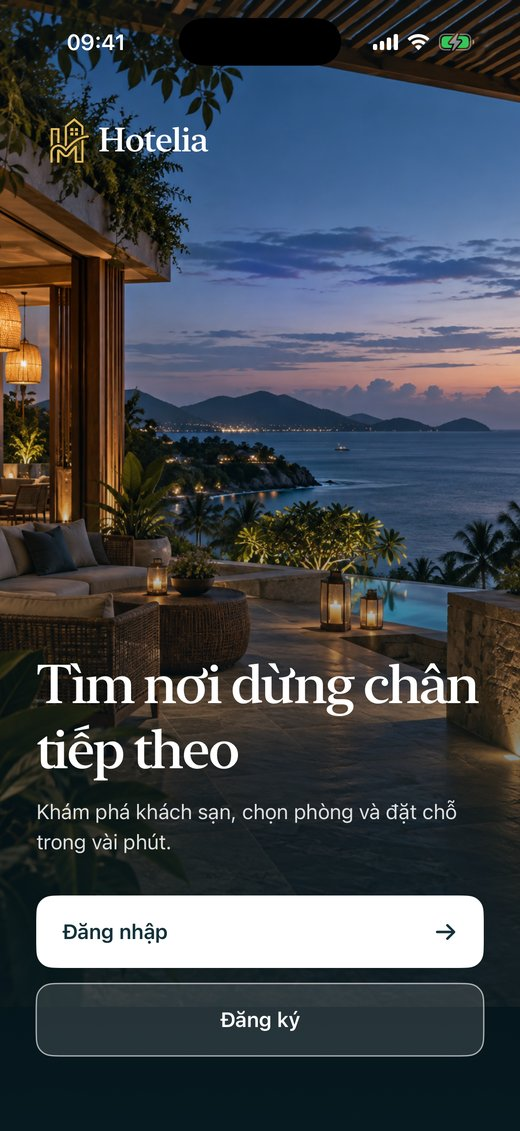
\includegraphics[width=0.3\linewidth]{figures/shots/vi-01-welcome.jpg}}\hfill
\subcaptionbox{Đăng ký}{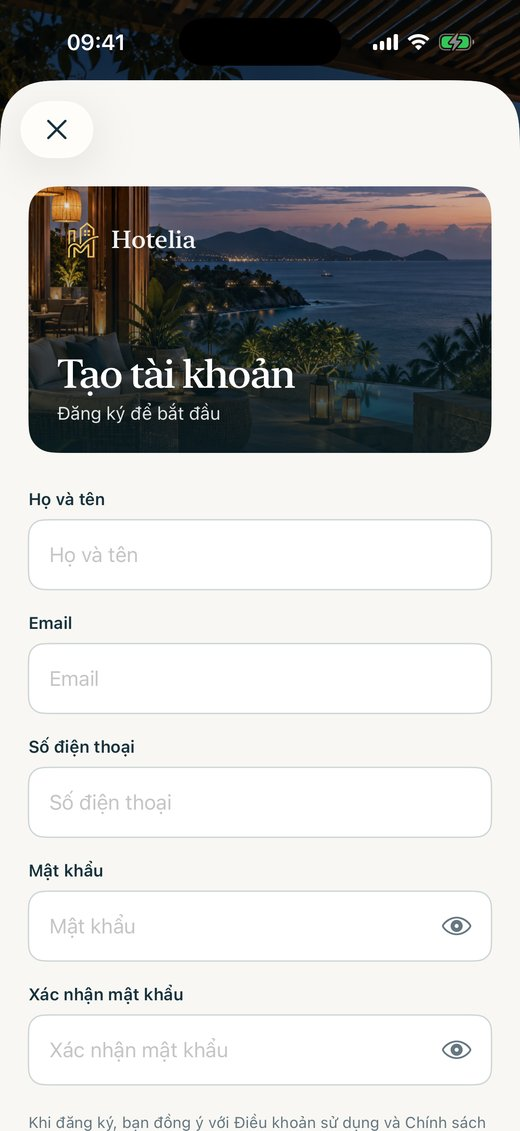
\includegraphics[width=0.3\linewidth]{figures/shots/vi-02-register.jpg}}\hfill
\subcaptionbox{Đăng nhập}{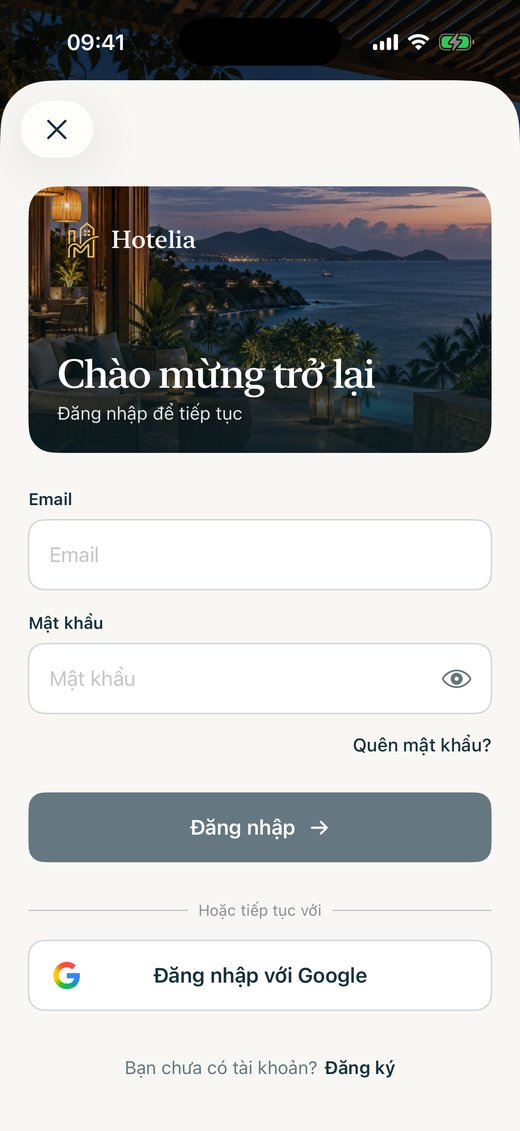
\includegraphics[width=0.3\linewidth]{figures/shots/vi-03-login.jpg}}
\caption{Màn hình chào mừng, đăng ký và đăng nhập}\label{fig:scr-auth}
\end{figure}

\paragraph{Khám phá và gợi ý.} \Cref{fig:scr-explore} là màn Khám phá. Phần đầu có ô tìm điểm đến, bộ chọn ngày, số khách và bộ lọc; tiếp theo là băng chuyền điểm đến và thẻ thời tiết. Cuộn xuống là hàng ``Đề xuất cho bạn''. Với tài khoản đã có lịch sử đặt phòng, dòng mô tả là ``Dựa trên khách sạn bạn đã xem và booking đã xác nhận''. Phần ``Xếp hạng tham khảo'' phân biệt khách sạn có điểm từ đánh giá đã xác minh (nhãn ``Điểm'') với khách sạn chỉ có điểm biên tập (nhãn ``Điểm Hotelia'').

\begin{figure}[H]
\centering
\subcaptionbox{Khám phá, thời tiết}{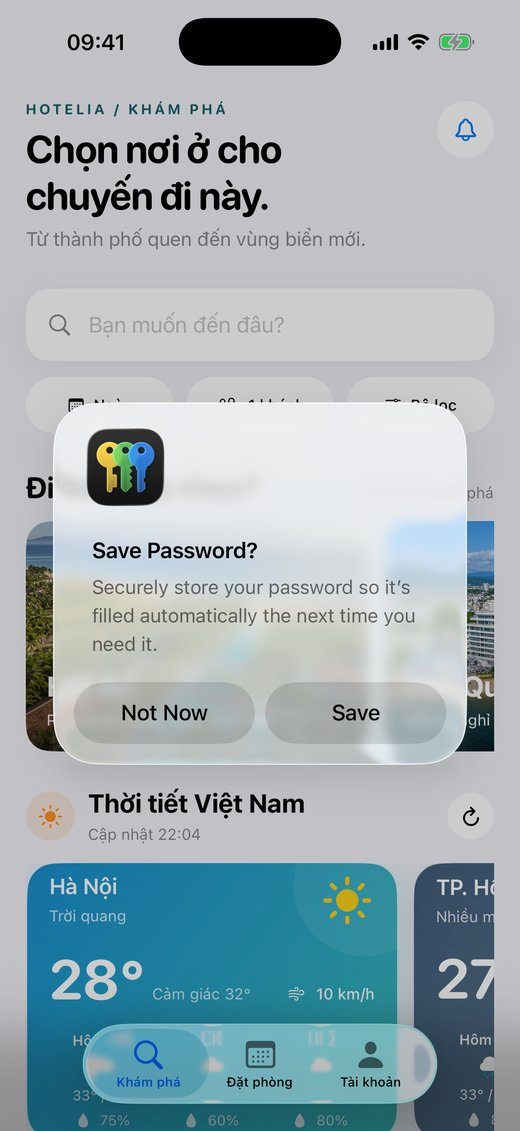
\includegraphics[width=0.3\linewidth]{figures/shots/vi-04-explore.jpg}}\hfill
\subcaptionbox{Đề xuất cho bạn}{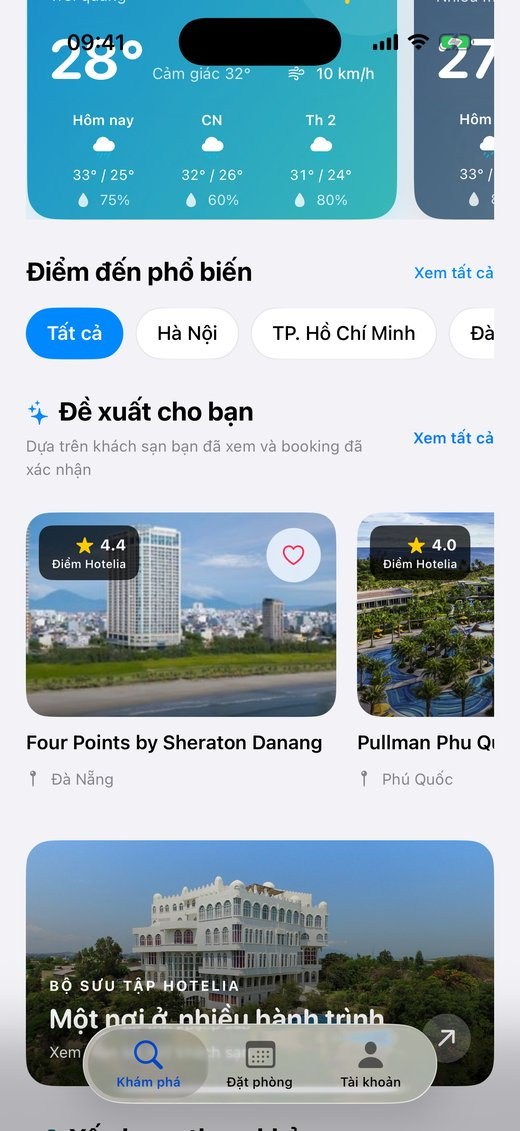
\includegraphics[width=0.3\linewidth]{figures/shots/vi-05-recommend.jpg}}\hfill
\subcaptionbox{Xếp hạng tham khảo}{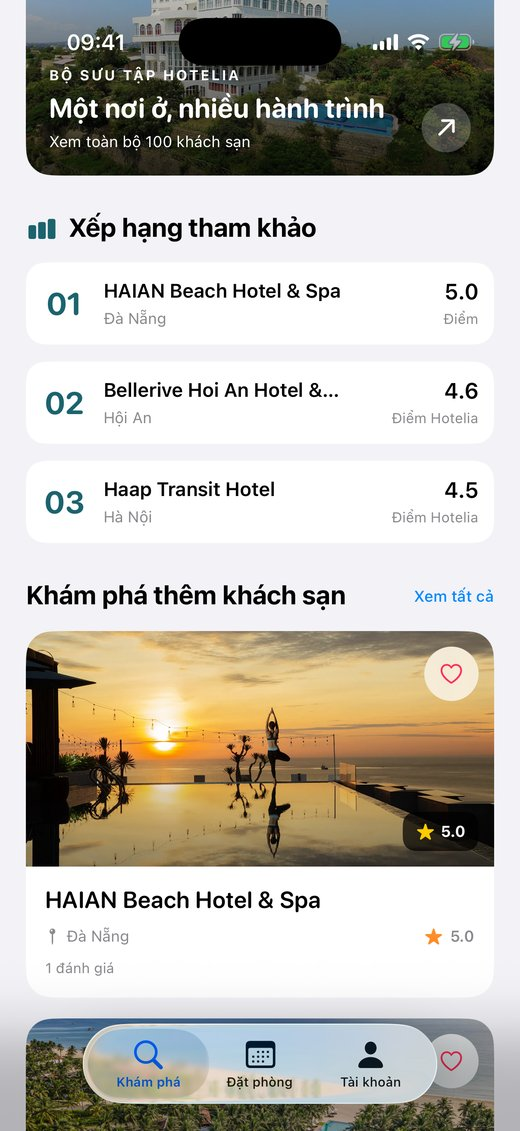
\includegraphics[width=0.3\linewidth]{figures/shots/vi-08-ranking.jpg}}
\caption{Màn Khám phá, thẻ thời tiết và hàng gợi ý cá nhân hóa}\label{fig:scr-explore}
\end{figure}

\paragraph{Chi tiết khách sạn.} \Cref{fig:scr-detail} gồm ảnh, hạng sao, trạng thái ``Đang nhận đặt phòng'', địa chỉ, mô tả, tiện ích, đánh giá và chính sách giờ nhận/trả phòng. Đánh giá đã xác minh (có ngày và phản hồi của khách sạn) được tách khỏi mục ``Nhận xét Hotelia'', mục này kèm dòng chú thích rằng đây không phải đánh giá của khách đã lưu trú.

\begin{figure}[H]
\centering
\subcaptionbox{Thông tin khách sạn}{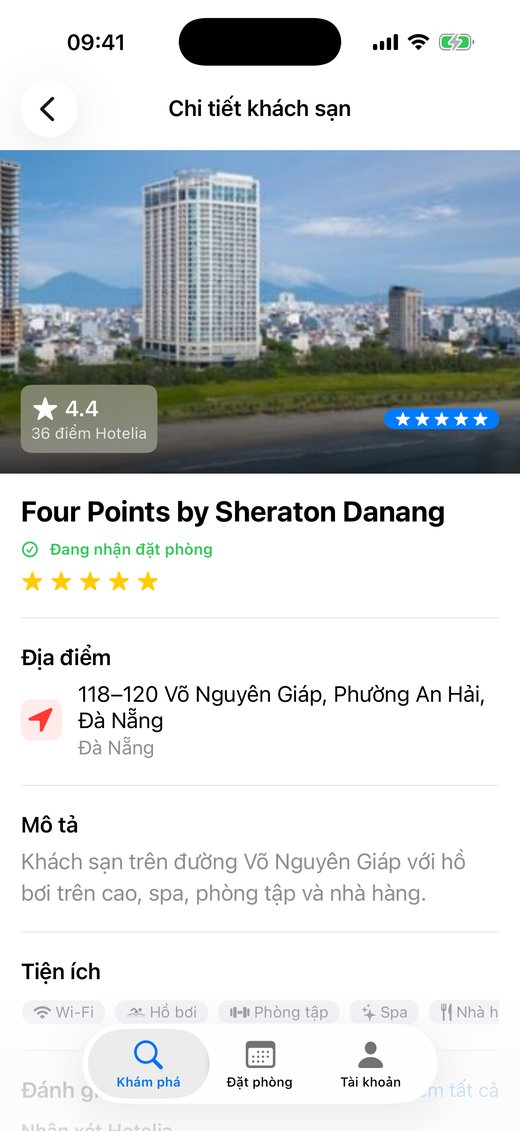
\includegraphics[width=0.3\linewidth]{figures/shots/vi-06-detail.jpg}}\hfill
\subcaptionbox{Đánh giá và phản hồi}{
\includegraphics[width=0.3\linewidth]{figures/shots/vi-09-reviews.jpg}}\hfill
\subcaptionbox{Chính sách, đặt phòng}{
\includegraphics[width=0.3\linewidth]{figures/shots/vi-07-detail-policy.jpg}}
\caption{Màn chi tiết khách sạn}\label{fig:scr-detail}
\end{figure}

\paragraph{Chọn phòng và đặt phòng.} \Cref{fig:scr-booking} là màn đặt phòng. Mỗi loại phòng hiển thị ảnh, sức chứa, tiện nghi, giá mỗi đêm và trạng thái chọn. Hai bộ chọn ngày nhận và ngày trả được xếp dọc; cách bố trí này sửa lỗi tràn ngang do chuỗi ngày tiếng Việt dài (\cref{sec:test-ui}). Phần cuối hiển thị tạm tính và các ghi chú về thời gian giữ phòng, chính sách hủy.

\begin{figure}[H]
\centering
\subcaptionbox{Chọn loại phòng}{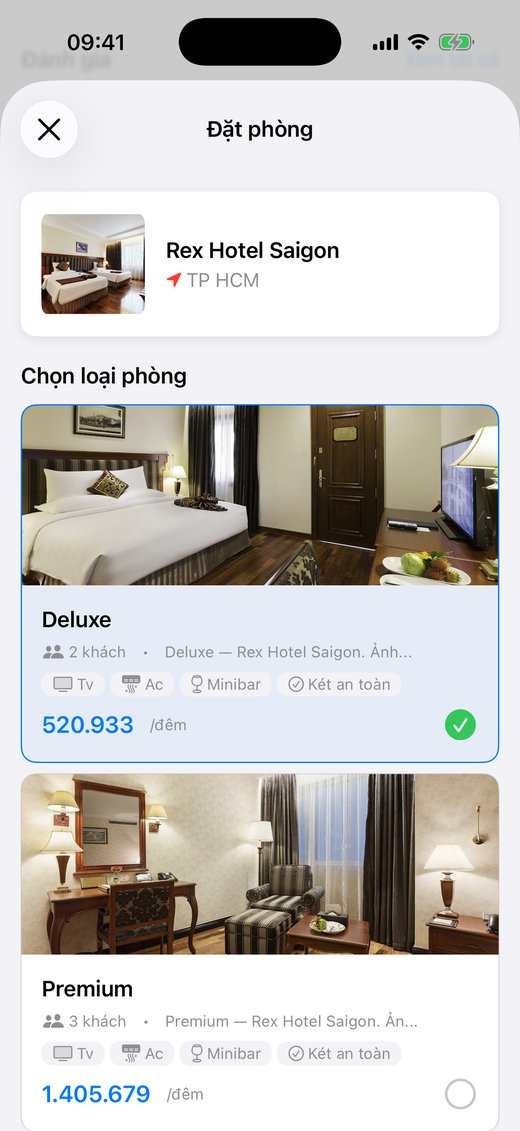
\includegraphics[width=0.3\linewidth]{figures/shots/vi-10-rooms.jpg}}\hfill
\subcaptionbox{Ngày, số khách}{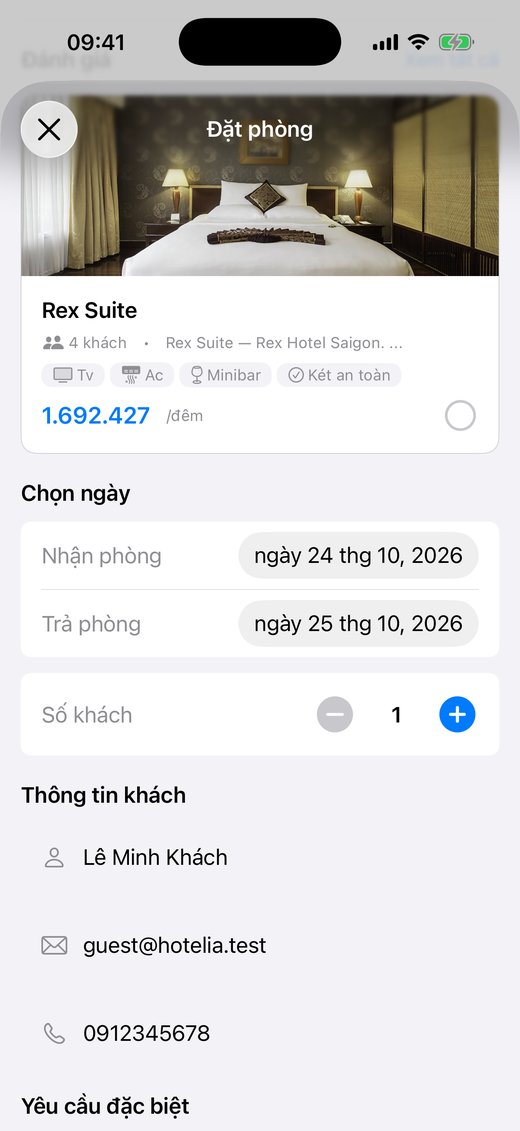
\includegraphics[width=0.3\linewidth]{figures/shots/vi-11-dates.jpg}}\hfill
\subcaptionbox{Đã giữ phòng}{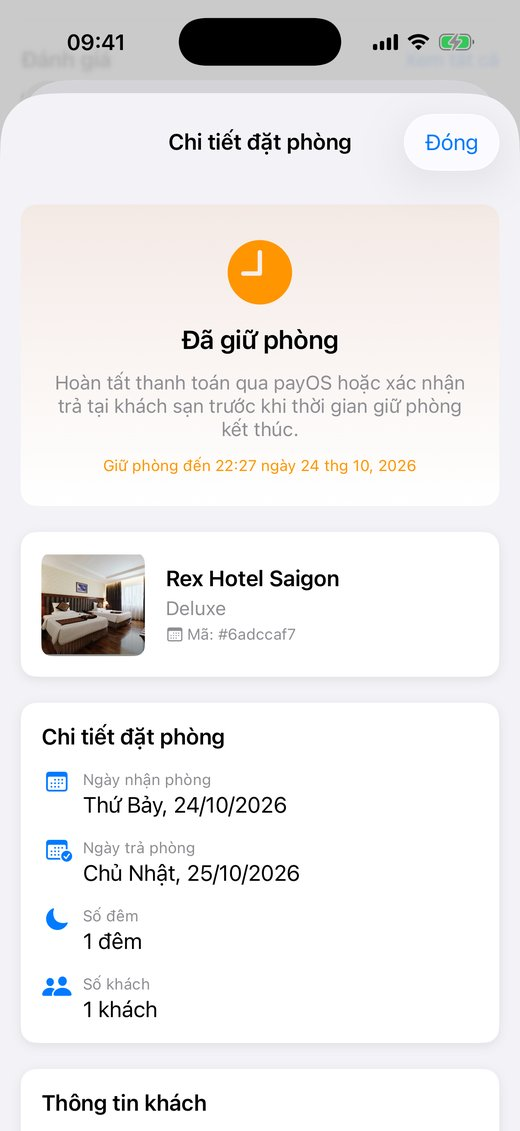
\includegraphics[width=0.3\linewidth]{figures/shots/vi-12-hold.jpg}}
\caption{Luồng chọn phòng, chọn ngày và giữ phòng}\label{fig:scr-booking}
\end{figure}

\paragraph{Thanh toán.} \Cref{fig:scr-payment} là phần thanh toán của chi tiết đặt phòng. Ảnh (b) cho thấy hành vi khi máy chủ chưa cấu hình khóa payOS: ứng dụng hiển thị ``Kênh thanh toán payOS chưa được cấu hình'' do máy chủ trả mã 503. Hệ thống không tạo đơn thanh toán nào. Ảnh (c) là lịch sử sau khi khách chọn ``Thanh toán tại khách sạn'': đặt phòng chuyển sang ``Đã xác nhận''.

\begin{figure}[H]
\centering
\subcaptionbox{Phương thức thanh toán}{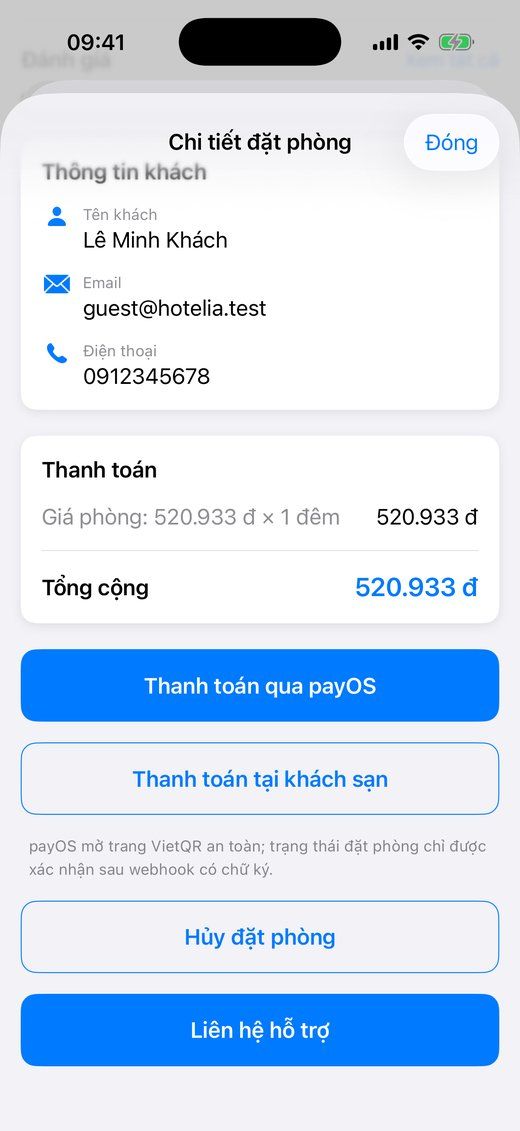
\includegraphics[width=0.3\linewidth]{figures/shots/vi-13-payment.jpg}}\hfill
\subcaptionbox{payOS chưa cấu hình}{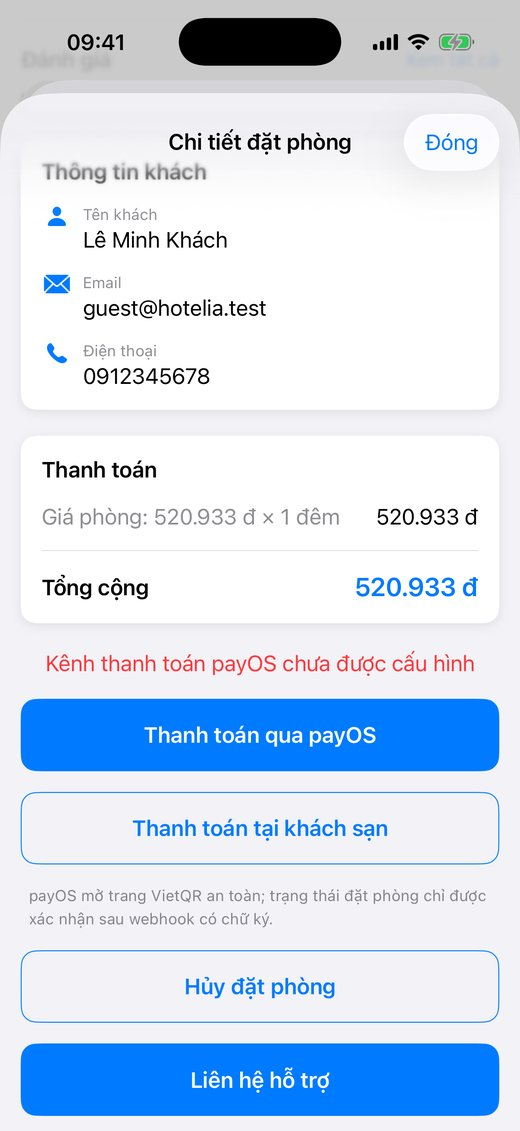
\includegraphics[width=0.3\linewidth]{figures/shots/vi-14-payos-unconfigured.jpg}}\hfill
\subcaptionbox{Đã xác nhận}{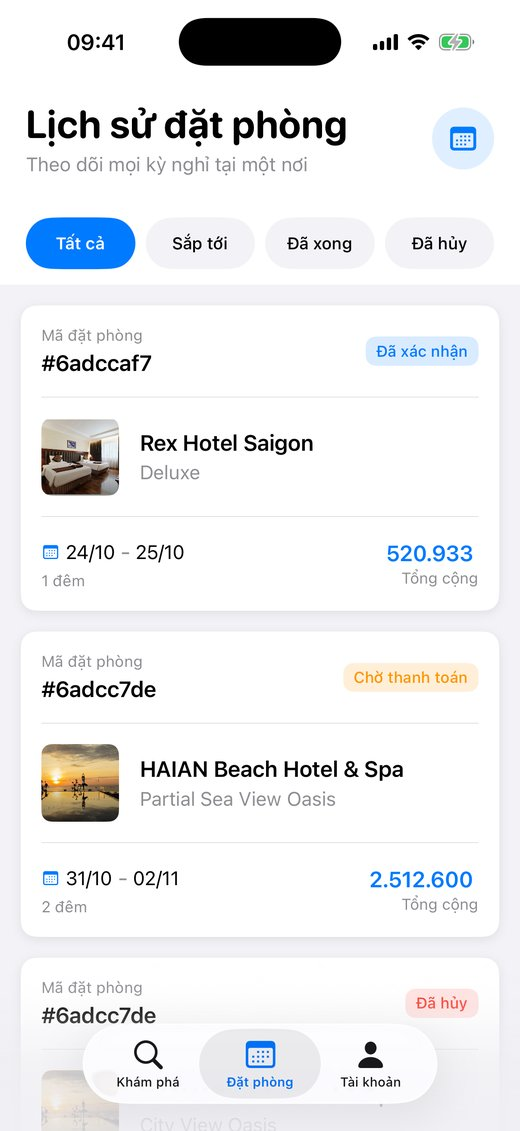
\includegraphics[width=0.3\linewidth]{figures/shots/vi-15-history.jpg}}
\caption{Thanh toán và xác nhận đặt phòng}\label{fig:scr-payment}
\end{figure}

\paragraph{Lịch sử đặt phòng và tài khoản.} \Cref{fig:scr-account} gồm lịch sử với nhiều trạng thái (đã nhận phòng, đã trả phòng), màn tài khoản và lựa chọn ngôn ngữ. Màn tài khoản là lối vào cho khách sạn đã lưu, đăng ký làm đối tác, hồ sơ, thông báo, bảo mật, ngôn ngữ, trợ giúp và màn quản lý dành cho chủ khách sạn/quản trị viên.

\begin{figure}[H]
\centering
\subcaptionbox{Trạng thái đặt phòng}{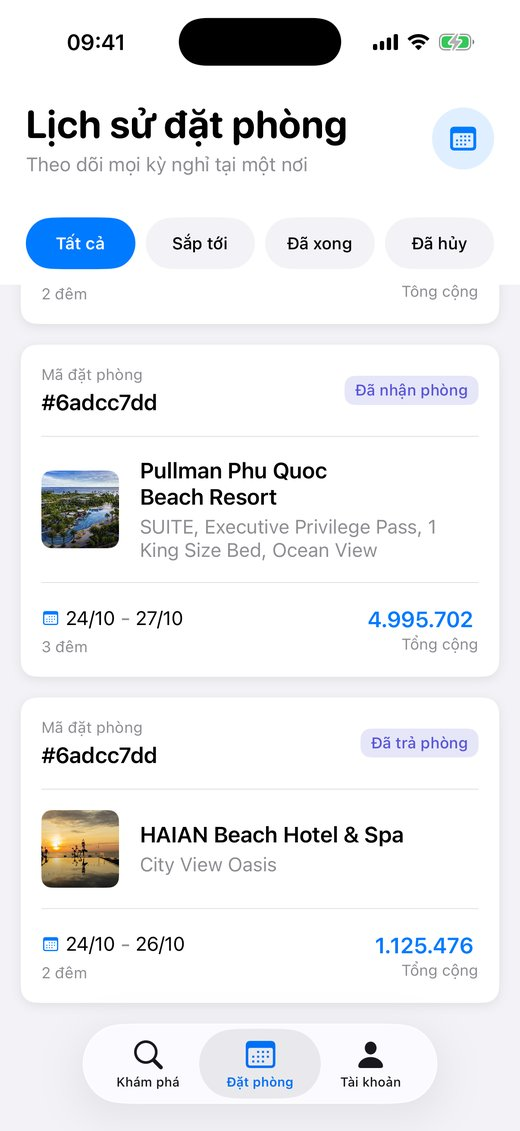
\includegraphics[width=0.3\linewidth]{figures/shots/vi-16-history-states.jpg}}\hfill
\subcaptionbox{Tài khoản}{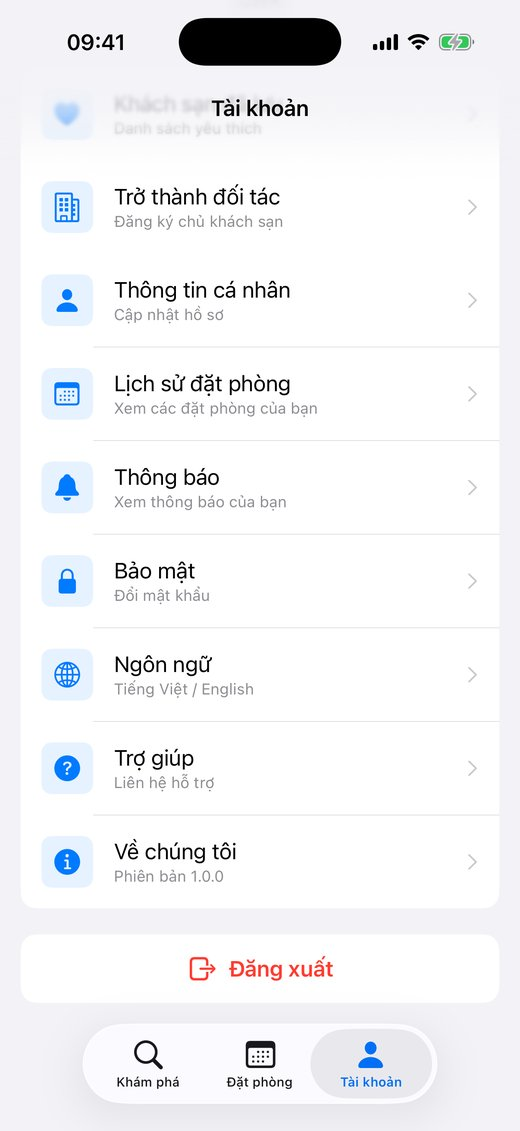
\includegraphics[width=0.3\linewidth]{figures/shots/vi-18-profile-menu.jpg}}\hfill
\subcaptionbox{Ngôn ngữ}{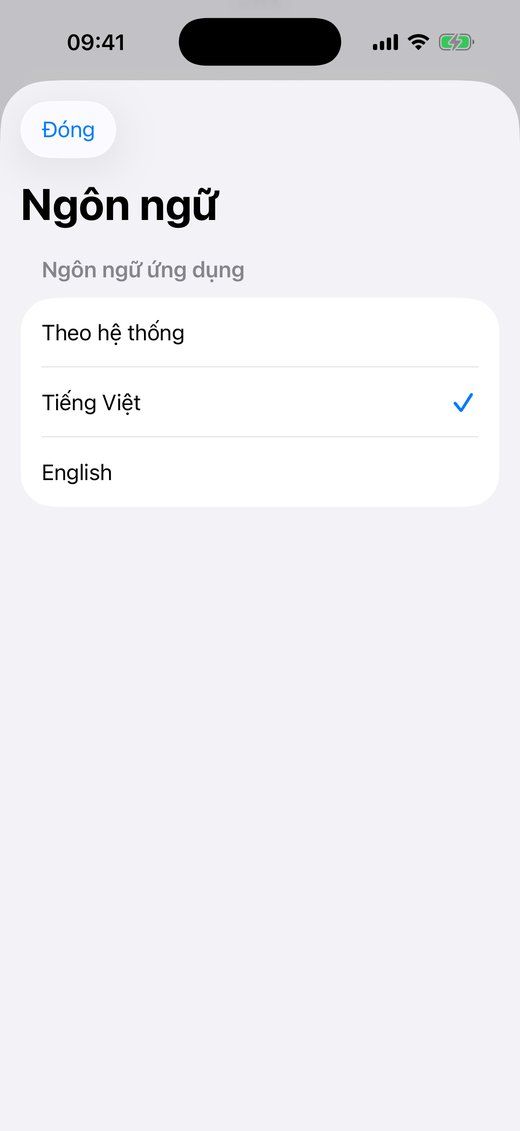
\includegraphics[width=0.3\linewidth]{figures/shots/vi-19-language.jpg}}
\caption{Lịch sử đặt phòng, tài khoản và chọn ngôn ngữ}\label{fig:scr-account}
\end{figure}

\paragraph{Giao diện tiếng Anh.} \Cref{fig:scr-english} là cùng các màn hình khi chọn tiếng Anh. Định dạng số đổi theo ngôn ngữ (``520,933'' thay vì ``520.933''). Nhãn trạng thái được dịch, kể cả ``Expired'' của đặt phòng đã hết hạn giữ.

\begin{figure}[H]
\centering
\subcaptionbox{Welcome}{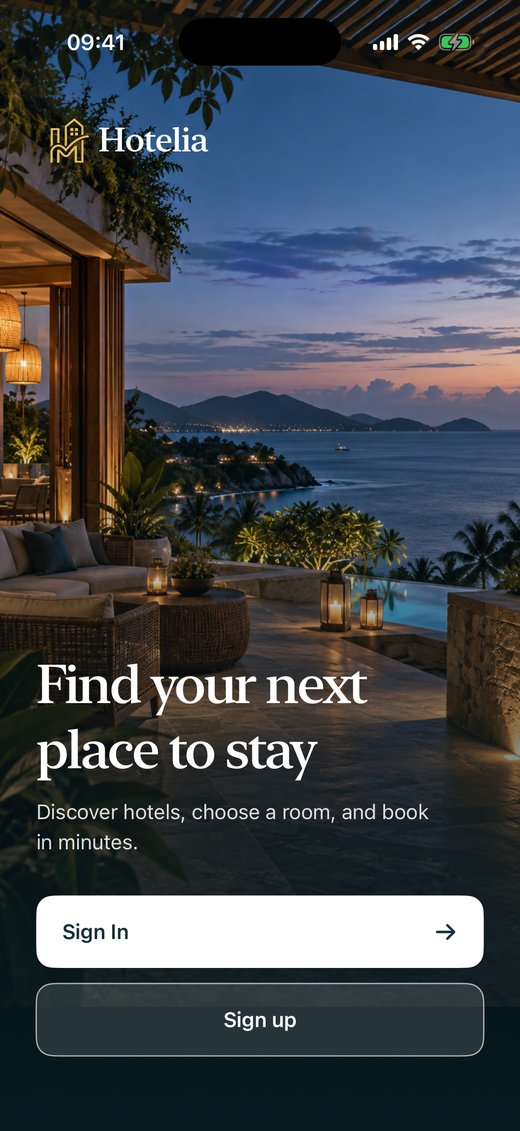
\includegraphics[width=0.3\linewidth]{figures/shots/en-01-welcome.jpg}}\hfill
\subcaptionbox{Explore}{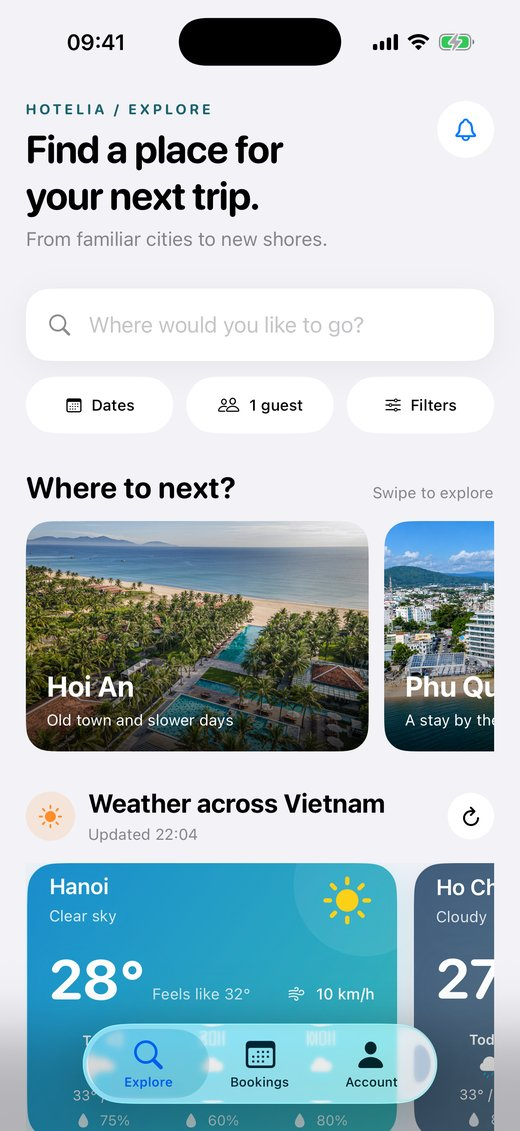
\includegraphics[width=0.3\linewidth]{figures/shots/en-04-explore.jpg}}\hfill
\subcaptionbox{Booking history}{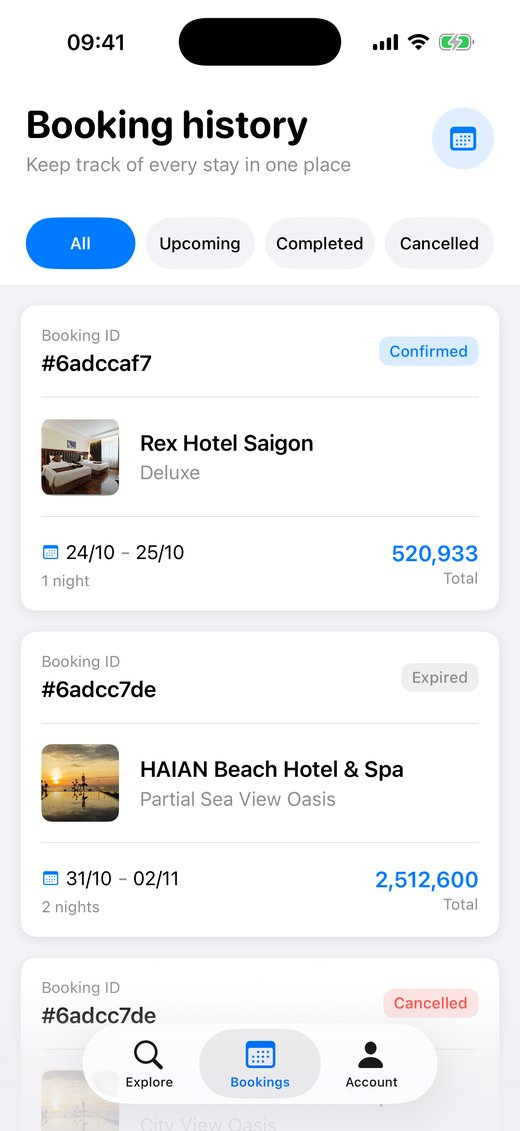
\includegraphics[width=0.3\linewidth]{figures/shots/en-05-history.jpg}}
\caption{Giao diện tiếng Anh của ứng dụng}\label{fig:scr-english}
\end{figure}

\section{Cài đặt máy chủ NestJS}\label{sec:impl-backend}

\subsection{Khởi động và cấu hình}

Tệp \code{main.ts} cấu hình các thành phần toàn cục:
\begin{itemize}
\item CORS: ở môi trường vận hành chỉ chấp nhận các nguồn khai báo trong \code{CORS\_ORIGINS}; ở môi trường phát triển chấp nhận thêm các cổng localhost của Vite.
\item Tiền tố \code{/api}, phiên bản URI mặc định \code{v1}.
\item \code{ValidationPipe} với \code{whitelist}, \code{forbidNonWhitelisted}, \code{transform}.
\item \code{HttpExceptionFilter}; thư mục ảnh tĩnh \code{/media/} không liệt kê thư mục và từ chối tệp ẩn.
\item Tài liệu Swagger, chỉ bật ở môi trường phát triển.
\end{itemize}
Hàm \code{validateEnvironment} kiểm tra cấu hình ngay khi khởi động. Máy chủ từ chối chạy ở môi trường vận hành nếu \code{JWT\_SECRET} ngắn hơn 32 ký tự hoặc trông như giá trị mẫu, nếu thiếu \code{CORS\_ORIGINS}, hoặc nếu chỉ có một phần trong ba khóa payOS. Bốn ca kiểm thử trong \code{env.validation.spec.ts} kiểm chứng các điều kiện này.

\subsection{Xác thực và phân quyền}\label{sec:impl-auth}

\Cref{lst:tokens} là hàm phát hành token. Trong quá trình viết báo cáo, việc đối chiếu với RFC 8725 \cite{rfc8725} cho thấy phiên bản cũ ký access token và refresh token bằng cùng khóa và cùng nội dung. Hệ quả là một refresh token có hạn 7 ngày cũng được \code{JwtStrategy} chấp nhận như access token. Bản sửa thêm claim \code{typ} vào mỗi token. \code{JwtStrategy} từ chối token có \code{typ = refresh} (\cref{lst:jwt}); điểm cuối làm mới từ chối token có \code{typ = access}. Token phát hành trước bản sửa không có \code{typ} và vẫn được chấp nhận cho tới khi hết hạn, để người dùng đang đăng nhập không bị đăng xuất đột ngột. Bốn ca kiểm thử mới kiểm chứng hành vi này.

Khi bổ sung chức năng thu hồi phiên lúc đăng xuất, báo cáo phát hiện thêm một lỗi trong cách lưu refresh token. Phiên bản cũ lưu \code{bcrypt(refreshToken)}, nhưng bcrypt chỉ đọc 72 byte đầu của đầu vào. Mọi refresh token của cùng một người dùng có chung 72 byte đầu (phần header và claim \code{sub}), nên token cũ vẫn khớp với bản băm của token mới và việc xoay vòng không vô hiệu hóa được token cũ. Ngoài ra, hai token phát hành trong cùng một giây có nội dung giống hệt nhau. Bản sửa gồm ba phần: (i) lưu bản băm SHA-256 của toàn bộ token và so sánh bằng \code{timingSafeEqual}; vì refresh token là chuỗi ngẫu nhiên dài do máy chủ ký nên không cần hàm băm chậm như với mật khẩu; (ii) thêm claim \code{jti} ngẫu nhiên vào mỗi refresh token (\cref{lst:tokens}); (iii) điểm cuối \code{POST /auth/logout} nhận chính refresh token cần thu hồi thay vì access token, nên đăng xuất vẫn có hiệu lực khi access token đã hết hạn. Bản băm bcrypt cũ vẫn được chấp nhận ở lần làm mới kế tiếp rồi được thay bằng SHA-256, để người dùng đang đăng nhập không bị đăng xuất khi triển khai. Ứng dụng iOS và bảng điều khiển gọi điểm cuối này ở nền khi người dùng đăng xuất.

\lstinputlisting[language=TypeScript, firstnumber=121, caption={Phát hành access token và refresh token có phân loại (\code{auth.service.ts})}, label={lst:tokens}]{code/auth-generate-tokens.ts}

\lstinputlisting[language=TypeScript, firstnumber=20, caption={Kiểm tra token ở mỗi yêu cầu (\code{jwt.strategy.ts})}, label={lst:jwt}]{code/jwt-validate.ts}

\code{JwtStrategy} đọc lại người dùng ở mỗi yêu cầu. Nhờ đó ba thay đổi có hiệu lực ngay: tài khoản bị khóa (\code{isActive = false}), mật khẩu vừa đổi (\code{tokenVersion} tăng), và vai trò vừa được nâng lên OWNER. Đổi lại, mỗi yêu cầu tốn thêm một truy vấn theo khóa chính. \code{RolesGuard} so khớp vai trò với danh sách khai báo bằng decorator \code{@Roles}. Kiểm tra quyền sở hữu được viết tường minh trong từng dịch vụ, ví dụ \code{String(hotel.ownerId) !== ownerId}.

\subsection{Máy trạng thái và giao dịch đặt phòng}\label{sec:impl-booking}

\Cref{lst:states} là bảng chuyển trạng thái được khai báo tường minh. \Cref{lst:rules} là các hàm thuần túy cài đặt quy tắc chiếm tồn kho, hết hạn giữ và đếm phòng trống theo đêm (\cref{eq:free-rooms}). Do là hàm thuần túy, chúng được kiểm thử trực tiếp mà không cần cơ sở dữ liệu.

\lstinputlisting[language=TypeScript, firstnumber=18, caption={Bảng chuyển trạng thái đặt phòng (\code{booking-state.service.ts})}, label={lst:states}]{code/booking-states.ts}

\lstinputlisting[language=TypeScript, firstnumber=3, caption={Quy tắc ngày, chiếm tồn kho và đếm phòng trống (\code{booking-rules.ts})}, label={lst:rules}]{code/booking-rules.ts}

\Cref{lst:create} là phần giao dịch của \code{BookingsService.create}. Ba chi tiết quan trọng là: (i) lệnh \code{findOneAndUpdate} tăng \code{inventoryVersion} nằm \emph{trước} truy vấn đếm, nên hai giao dịch đồng thời xung đột ngay tại tài liệu loại phòng; (ii) giá được lấy từ loại phòng trong giao dịch, không lấy từ yêu cầu; (iii) khối \code{catch} tra lại theo khóa lũy đẳng, vì khi hai yêu cầu cùng khóa chạy đồng thời, yêu cầu thua có thể gặp lỗi trùng chỉ mục duy nhất trong khi đặt phòng đã tồn tại.

\lstinputlisting[language=TypeScript, firstnumber=39, caption={Giao dịch tạo đặt phòng (\code{bookings.service.ts})}, label={lst:create}]{code/bookings-create-tx.ts}

Mọi thay đổi trạng thái sau đó đi qua hàm \code{transition}: cập nhật có điều kiện \code{\{\_id, status: trạng thái cũ\}}. Nếu không có tài liệu nào khớp, hàm đọc lại đặt phòng. Nếu trạng thái hiện tại đã là trạng thái đích, hàm trả về thành công; nếu không, hàm báo ``Booking đã thay đổi. Vui lòng tải lại''.

\subsection{Thanh toán và webhook}\label{sec:impl-payment}

\code{PayOSClient} bao thư viện \code{@payos/node} \cite{payosnode} với thời gian chờ 10 giây, tối đa 2 lần thử lại. Lỗi được chuyển thành mã HTTP có nghĩa: hết thời gian chờ thành 502 ``payOS không phản hồi trong thời gian cho phép'', thiếu cấu hình thành 503. \Cref{lst:verify} là hàm xác minh webhook. Thư viện tính lại HMAC-SHA256 bằng \code{checksumKey}; chữ ký sai làm webhook bị từ chối với mã 400.

\lstinputlisting[language=TypeScript, firstnumber=101, caption={Xác minh chữ ký webhook payOS (\code{payos.client.ts})}, label={lst:verify}]{code/payos-verify.ts}

\Cref{lst:webhook} là phần xử lý webhook đã xác minh. Webhook mẫu mà payOS gửi khi đăng ký địa chỉ webhook không khớp đơn nào và được trả lời ``đã xác minh'' mà không thay đổi dữ liệu. Webhook thật được xử lý trong một giao dịch: bỏ qua nếu thanh toán đã COMPLETED (lũy đẳng), dừng nếu số tiền lệch. Phần tiếp theo của giao dịch (không in ở đây) chuyển thanh toán sang COMPLETED; nếu đặt phòng còn PENDING\_PAYMENT thì chuyển sang CONFIRMED, hoặc sang CANCEL\_REQUESTED với lý do \code{PAYMENT\_AFTER\_HOLD\_EXPIRED} khi giữ phòng đã hết hạn; cuối cùng ghi thông báo cho khách.

\lstinputlisting[language=TypeScript, firstnumber=174, caption={Xử lý webhook payOS trong giao dịch (\code{payments.service.ts})}, label={lst:webhook}]{code/payments-webhook.ts}

Việc hoàn tiền chưa được cài đặt: \code{PaymentsService.refund} luôn trả 503 kèm thông điệp cần đối soát thủ công. Báo cáo ghi nhận đây là giới hạn (\cref{sec:limitations}).

\subsection{Nhật ký thao tác và giới hạn tần suất}

\code{AuditInterceptor} được đăng ký toàn cục. Sau mỗi yêu cầu POST, PUT, PATCH, DELETE thành công của người dùng đã đăng nhập (trừ nhóm \code{/auth/}), interceptor ghi \code{actorId}, \code{role}, \code{method}, \code{path} vào \code{audit\_logs}. Nội dung yêu cầu không được lưu, nên mật khẩu hay thông tin cá nhân không lọt vào nhật ký. Lỗi ghi nhật ký chỉ được cảnh báo, không làm hỏng yêu cầu chính. \code{ThrottlerGuard} giới hạn 100 yêu cầu mỗi 60 giây.

\section{Cài đặt bảng điều khiển React}\label{sec:impl-web}

\subsection{Cấu trúc và xác thực}

Bảng điều khiển gồm các thư mục \code{features/owner}, \code{features/admin}, \code{features/auth}, \code{components/ui} (Button, Card, Badge, StatCard, Input), \code{components/layout} (Sidebar, Layout), \code{lib/api/client.ts} và \code{lib/auth/AuthContext.tsx}. Client Axios gắn access token vào mọi yêu cầu. Khi gặp 401, client làm mới token một lần; các yêu cầu đồng thời dùng chung một promise làm mới (\code{refreshInFlight}), tương tự actor ở phía iOS. Thành phần \code{PrivateRoute} kiểm tra vai trò trước khi hiển thị nhánh \code{/owner/*} hoặc \code{/admin/*}.

\subsection{Màn hình chủ khách sạn}

\Cref{fig:web-owner} là các màn hình của chủ khách sạn, chụp ở độ phân giải 1440$\times$900. Bảng điều khiển tổng quan có bốn chỉ số (khách sạn, đã đăng, đặt phòng, đang lưu trú) và biểu đồ giá trị đặt phòng được xác nhận theo tháng. Màn ``Đơn đặt phòng'' liệt kê đặt phòng với nhãn trạng thái và thao tác nhận phòng, trả phòng, xác nhận hủy. Màn ``Đánh giá'' cho phép phản hồi đánh giá của khách.

\begin{figure}[H]
\centering
\subcaptionbox{Tổng quan khách sạn\label{fig:web-owner-dash}}{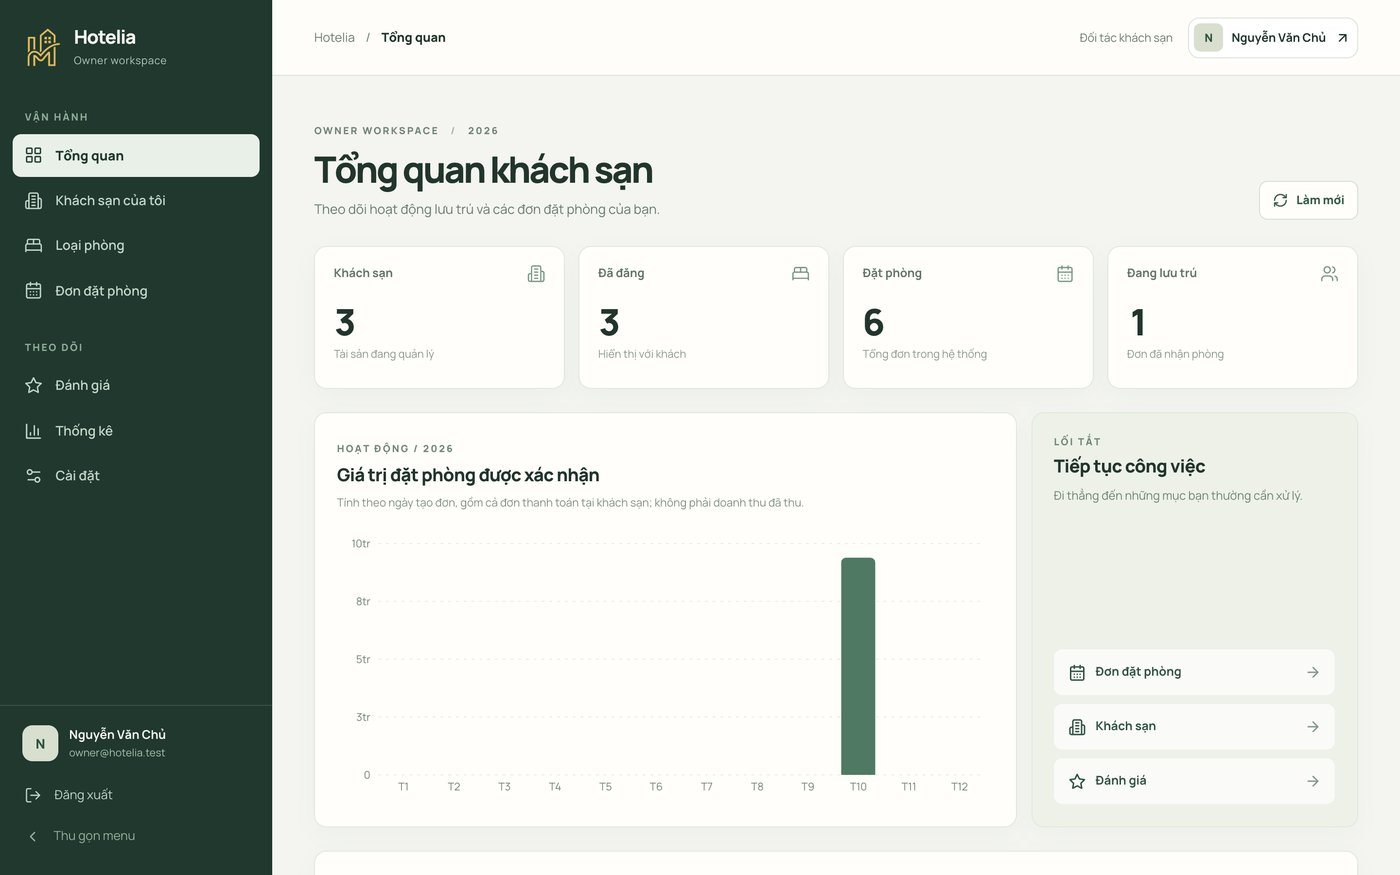
\includegraphics[width=0.49\linewidth]{figures/shots/web-02-owner-dashboard.jpg}}\hfill
\subcaptionbox{Khách sạn của tôi}{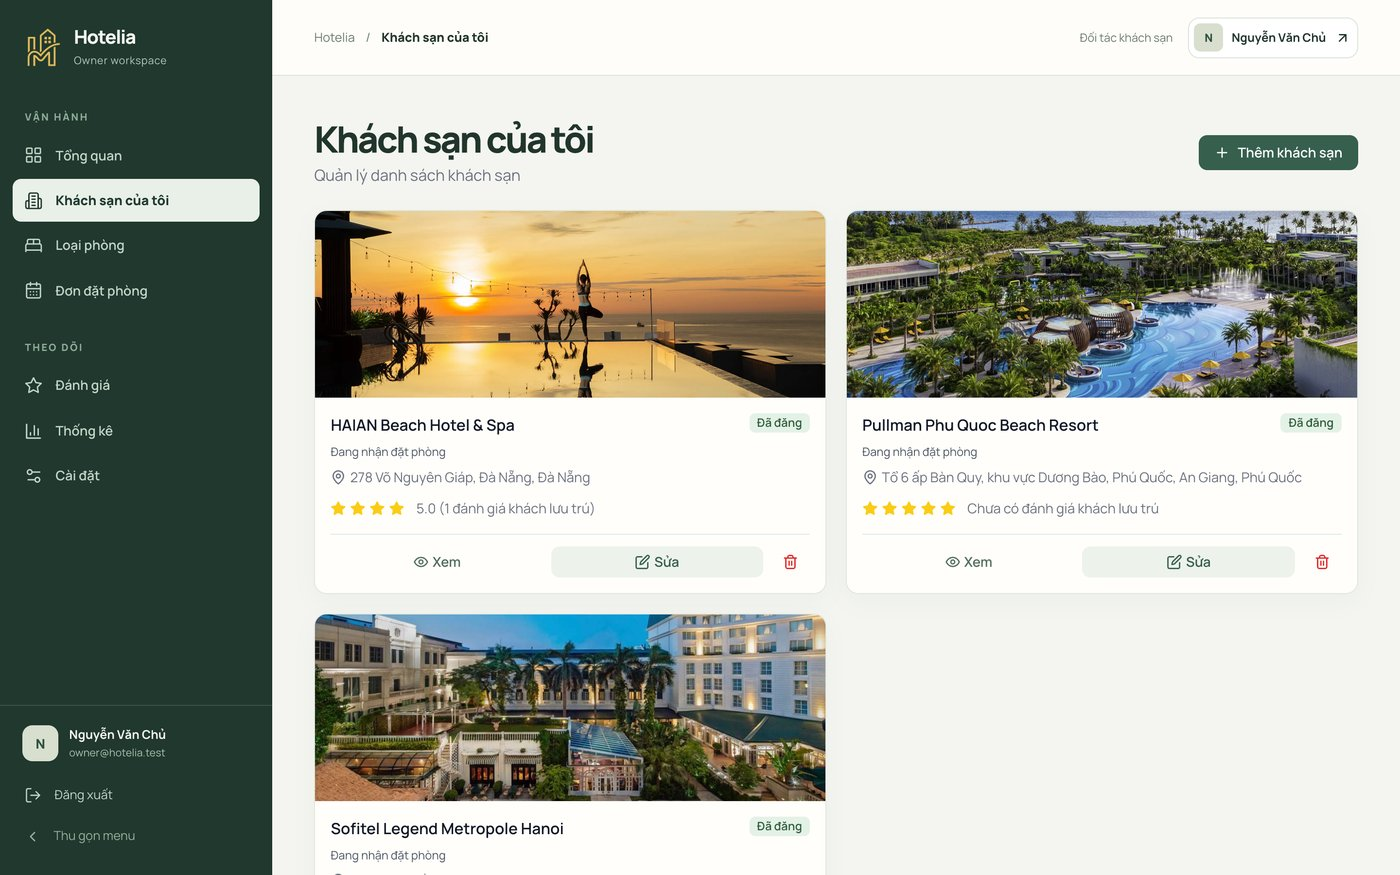
\includegraphics[width=0.49\linewidth]{figures/shots/web-03-owner-hotels.jpg}}\\[6pt]
\subcaptionbox{Đơn đặt phòng}{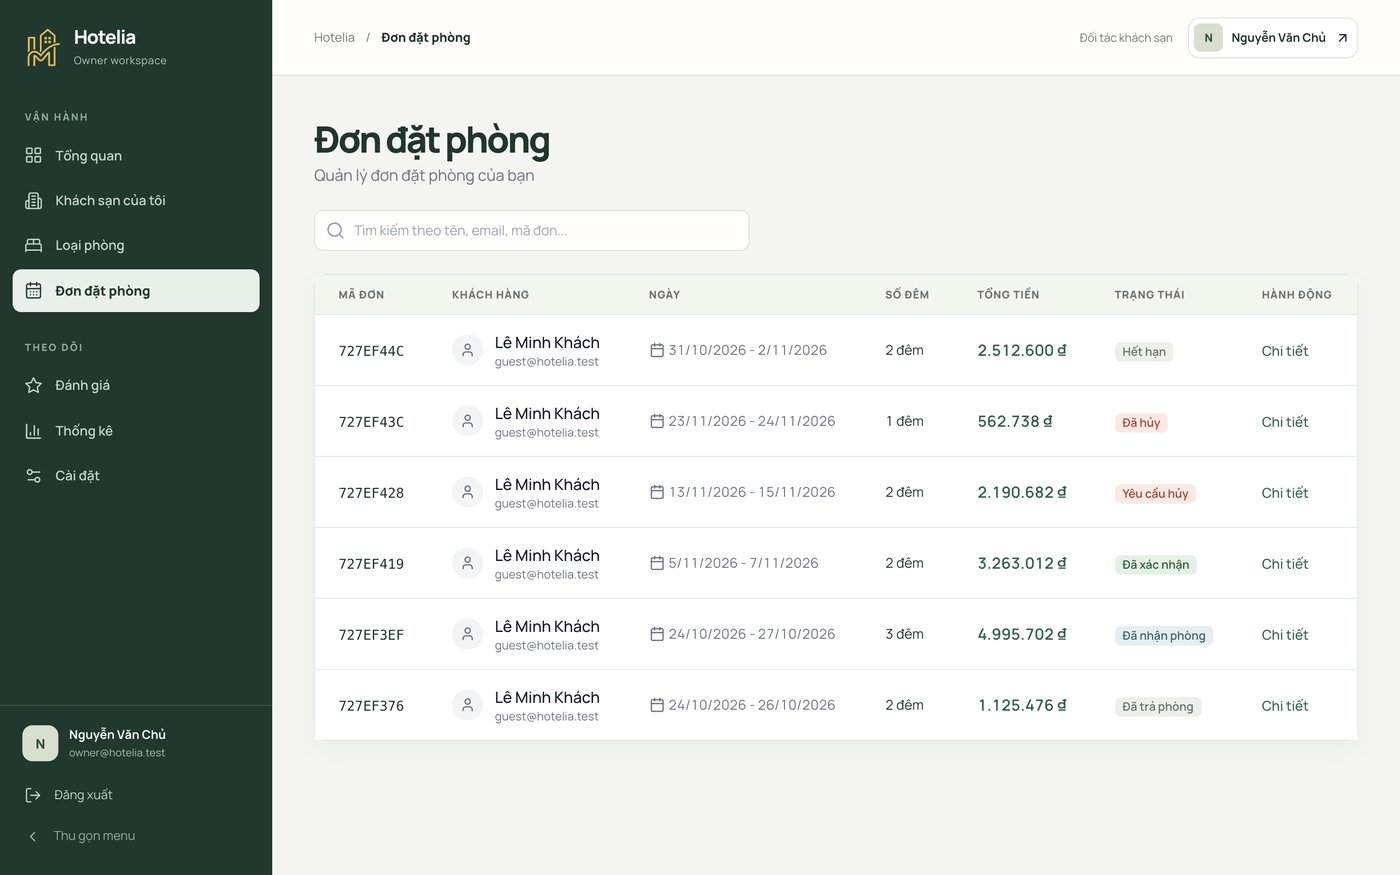
\includegraphics[width=0.49\linewidth]{figures/shots/web-04-owner-bookings.jpg}}\hfill
\subcaptionbox{Đánh giá và phản hồi}{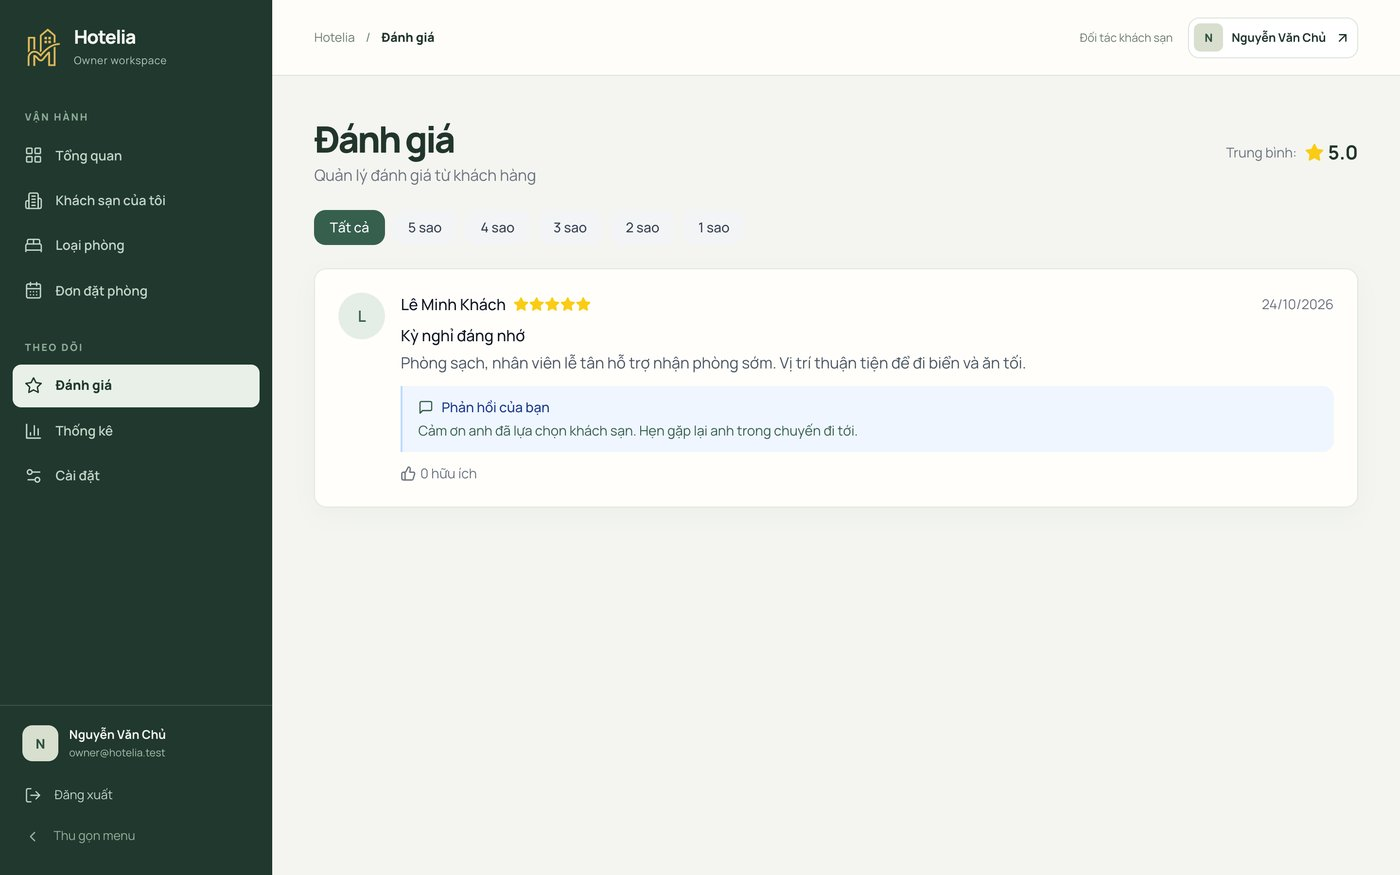
\includegraphics[width=0.49\linewidth]{figures/shots/web-05-owner-reviews.jpg}}
\caption{Bảng điều khiển của chủ khách sạn}\label{fig:web-owner}
\end{figure}

\subsection{Màn hình quản trị viên}

\Cref{fig:web-admin} là các màn hình của quản trị viên. Màn ``Chủ khách sạn'' hiển thị số hồ sơ chờ duyệt, đã duyệt, bị từ chối và nút duyệt/từ chối cho hồ sơ đang chờ. Màn ``Quản lý khách sạn'' có bộ lọc theo trạng thái và cho biết khách sạn nào đang nhận đặt phòng. Màn ``Thanh toán'' ghi rõ rằng giao dịch payOS chỉ được đánh dấu COMPLETED sau khi máy chủ xác thực chữ ký webhook, và đơn trả tại khách sạn không phải giao dịch đã thu tiền. Màn ``Nhật ký thao tác'' hiển thị tối đa 200 thao tác gần nhất.

\begin{figure}[H]
\centering
\subcaptionbox{Tổng quan hệ thống}{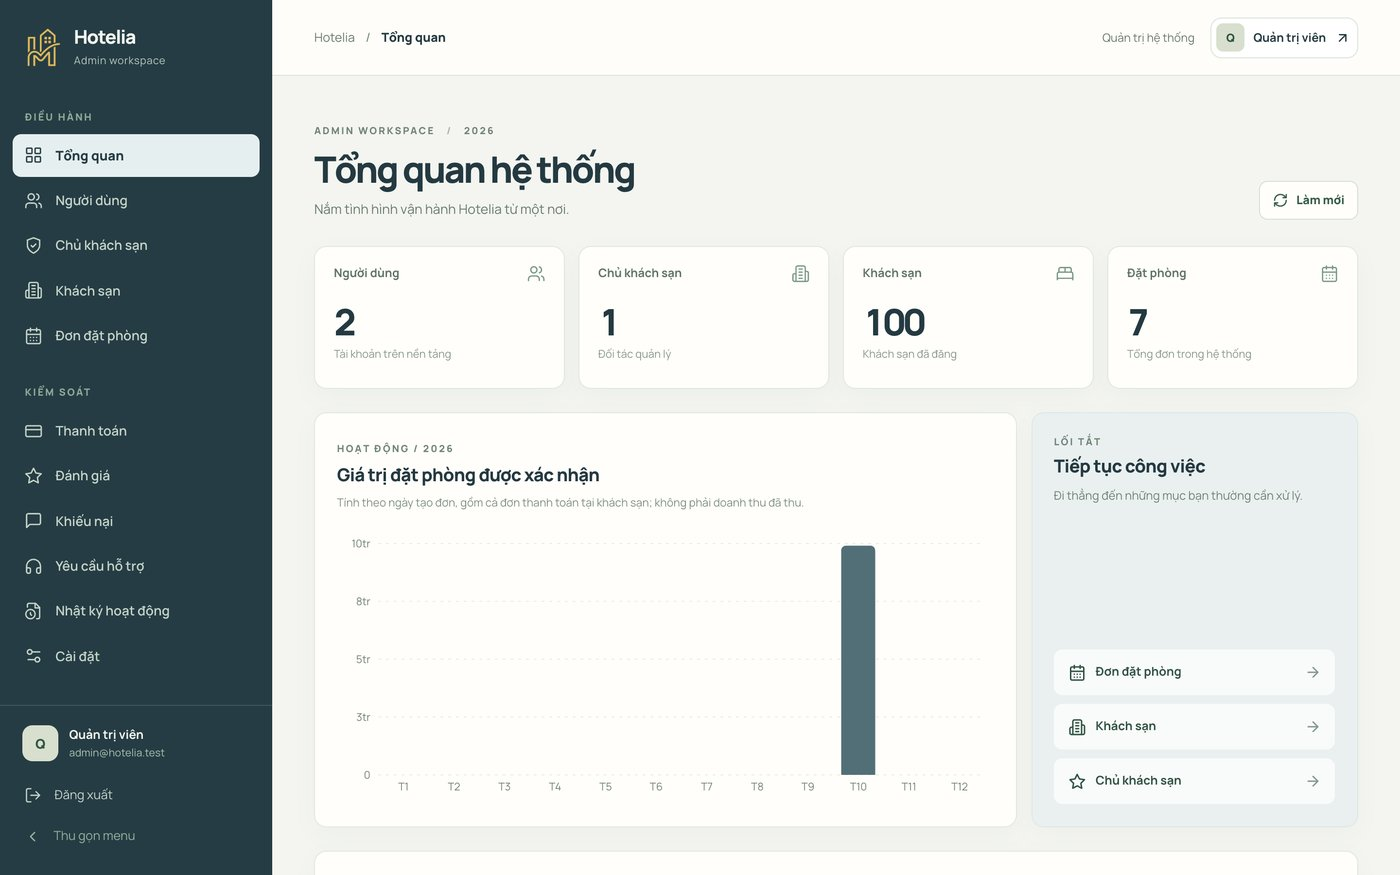
\includegraphics[width=0.49\linewidth]{figures/shots/web-06-admin-dashboard.jpg}}\hfill
\subcaptionbox{Duyệt chủ khách sạn}{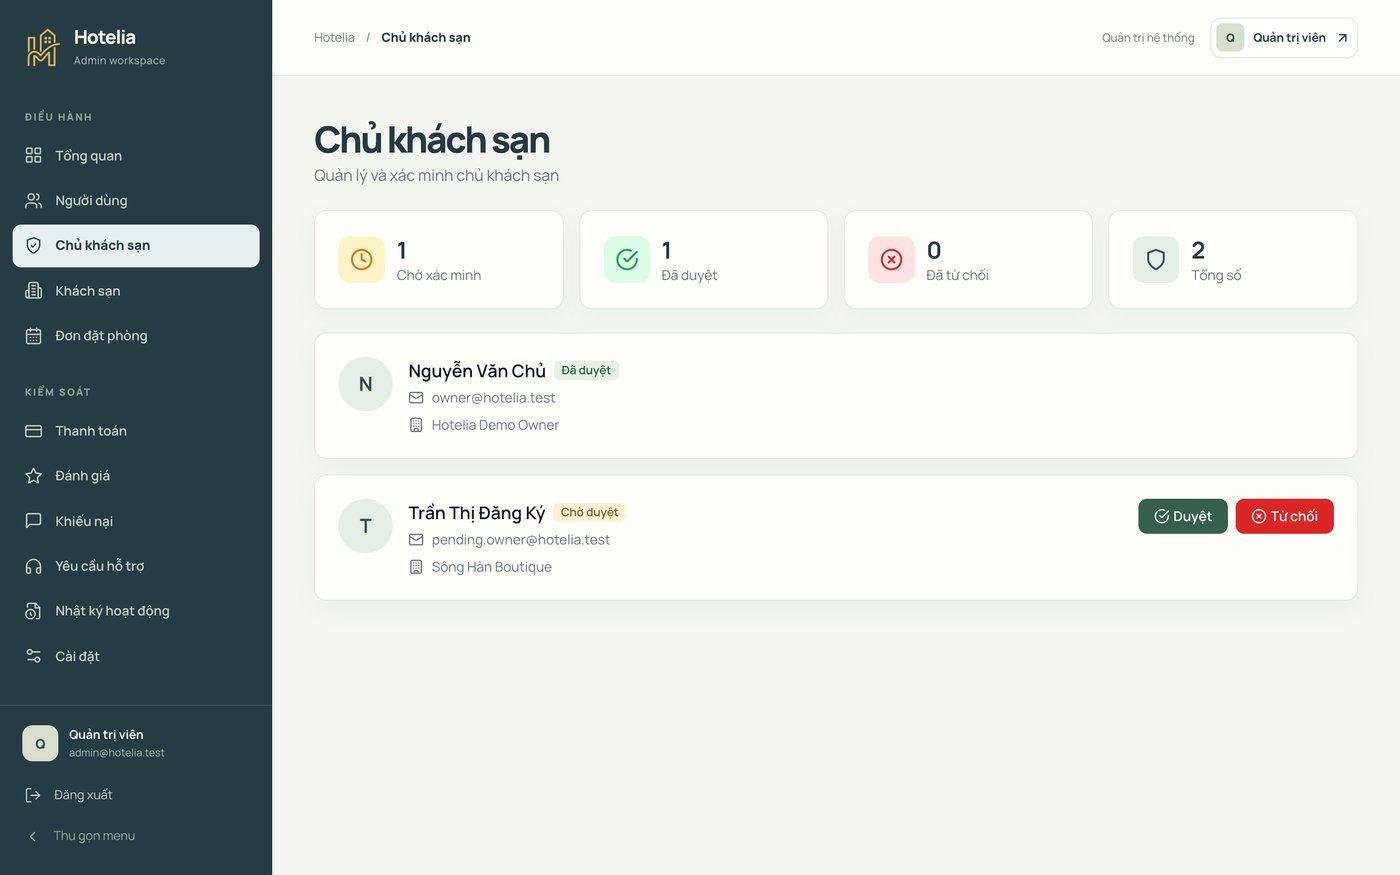
\includegraphics[width=0.49\linewidth]{figures/shots/web-07-admin-owners.jpg}}\\[6pt]
\subcaptionbox{Quản lý khách sạn}{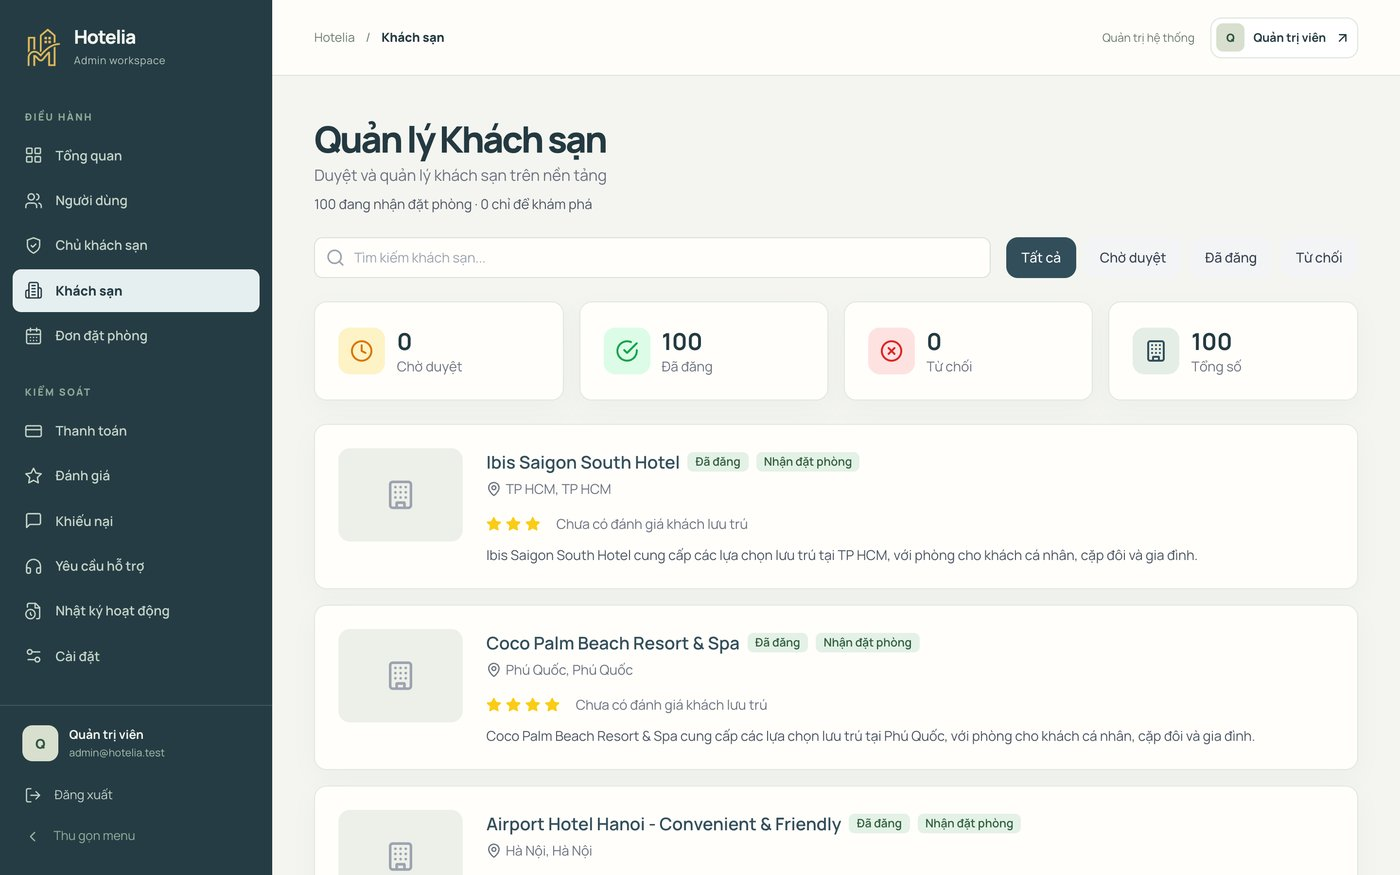
\includegraphics[width=0.49\linewidth]{figures/shots/web-08-admin-hotels.jpg}}\hfill
\subcaptionbox{Quản lý người dùng}{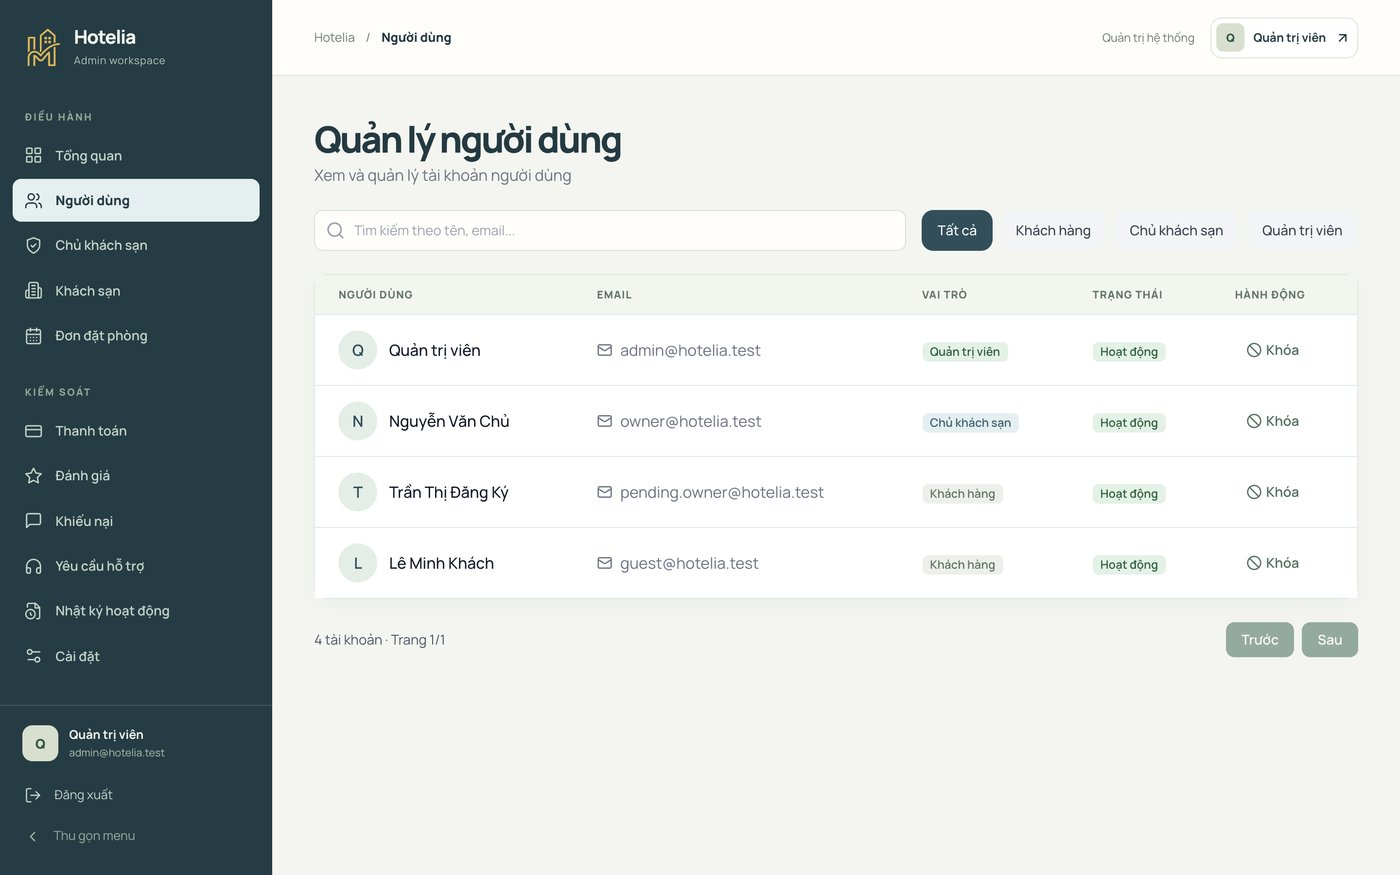
\includegraphics[width=0.49\linewidth]{figures/shots/web-09-admin-users.jpg}}\\[6pt]
\subcaptionbox{Thanh toán}{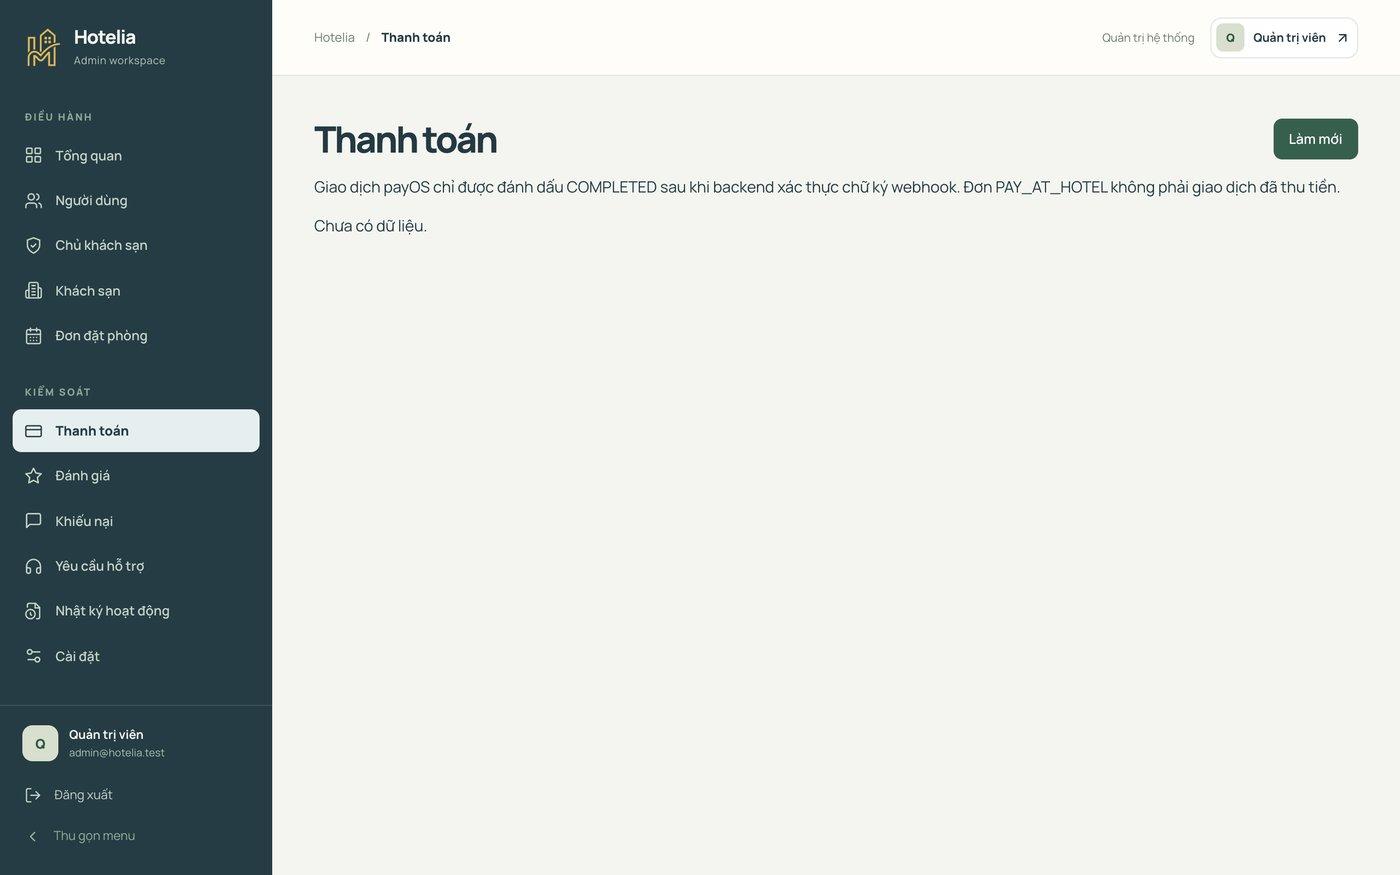
\includegraphics[width=0.49\linewidth]{figures/shots/web-11-admin-payments.jpg}}\hfill
\subcaptionbox{Nhật ký thao tác}{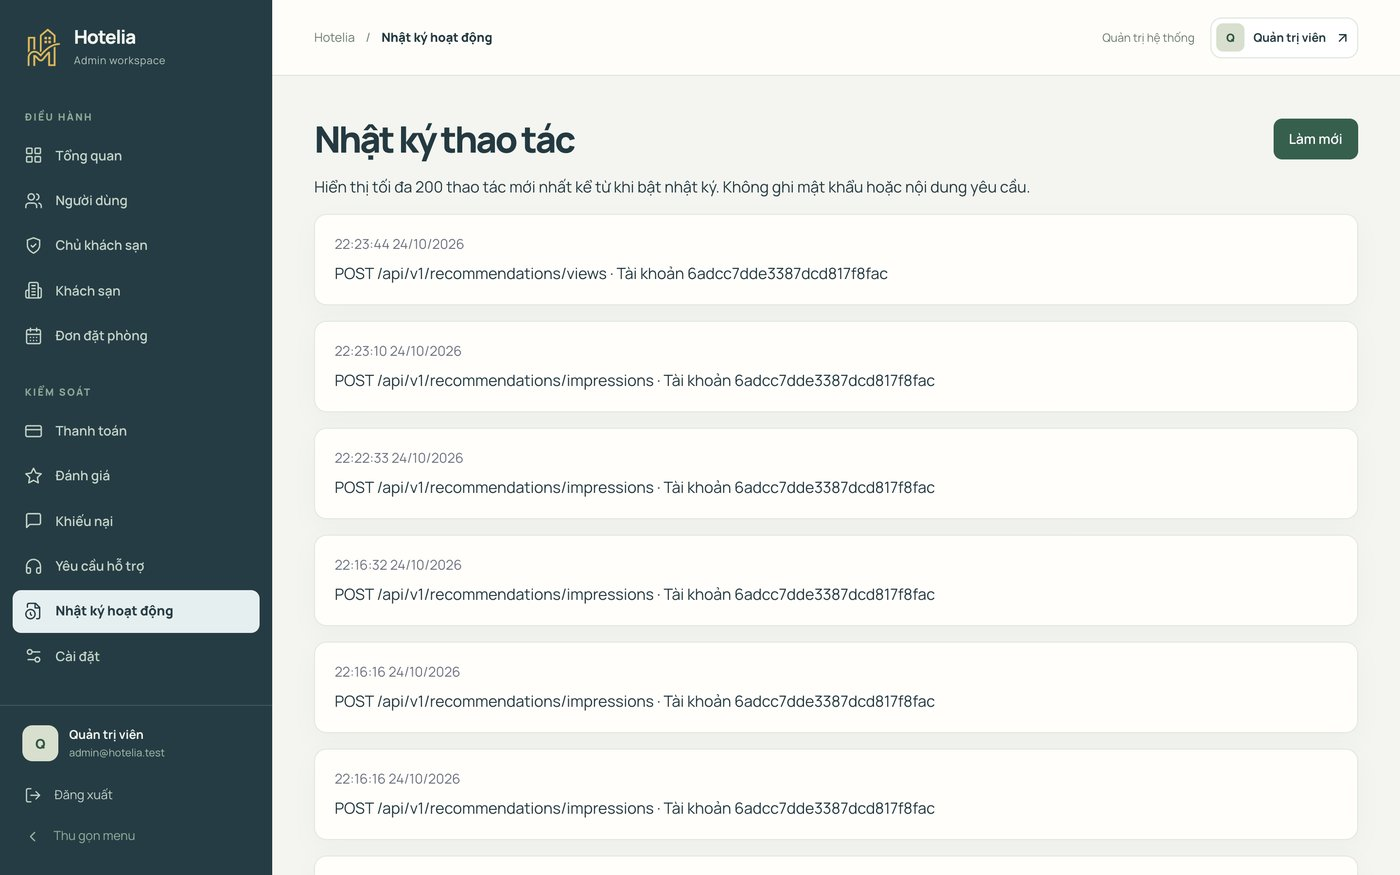
\includegraphics[width=0.49\linewidth]{figures/shots/web-13-admin-audit.jpg}}
\caption{Bảng điều khiển của quản trị viên}\label{fig:web-admin}
\end{figure}

\section{Cài đặt thành phần gợi ý}\label{sec:impl-rec}

\subsection{Đọc và chấm điểm mô hình LightGBM trong NestJS}

Tệp mô hình do LightGBM xuất (\code{dump\_model}) mô tả mỗi cây dưới dạng nút lồng nhau. Nút trong có \code{split\_feature}, \code{threshold}, \code{decision\_type} và \code{default\_left}; nút lá có \code{leaf\_value}. \Cref{lst:tree} là toàn bộ bộ chấm điểm: duyệt từng cây từ gốc tới lá rồi cộng các giá trị lá. Giá trị thiếu (NaN, vô cực) đi theo nhánh mặc định do LightGBM học được. Bộ chấm điểm chỉ chấp nhận phép so sánh \code{<=} (loại duy nhất xuất hiện với đặc trưng số) và ném lỗi với loại khác. Lỗi này khiến hệ thống chuyển sang bộ xếp hạng dự phòng thay vì trả điểm sai.

\lstinputlisting[language=TypeScript, firstnumber=31, caption={Chấm điểm cây LightGBM bằng TypeScript (\code{lightgbm-ranker.ts})}, label={lst:tree}]{code/lgbm-evaluate.ts}

\lstinputlisting[language=TypeScript, firstnumber=108, caption={Nạp và kiểm tra hợp đồng đặc trưng của mô hình}, label={lst:load}]{code/lgbm-load.ts}

Mô hình được nạp một lần khi khởi động (\cref{lst:load}). Nếu tệp thiếu, hỏng, sai danh sách đặc trưng hoặc không có cây, máy chủ ghi cảnh báo và tiếp tục chạy với bộ xếp hạng dự phòng. Tệp \code{nest-cli.json} khai báo \code{recommendations/models/*.json} là tài nguyên cần sao chép vào \code{dist}, để bản build Docker có tệp mô hình.

\subsection{Bảo đảm khớp giữa Python và TypeScript}

Lệch giữa huấn luyện và phục vụ là rủi ro lớn nhất của cách tiếp cận hai ngôn ngữ. Hai cơ chế được dùng để kiểm soát rủi ro này:
\begin{enumerate}
\item Khớp điểm số: tệp mô hình chứa 5 véc-tơ đặc trưng lấy từ tập kiểm tra cùng điểm do LightGBM Python tính. Kiểm thử Jest chấm lại bằng TypeScript và yêu cầu khớp tới 9 chữ số thập phân.
\item Khớp từng đặc trưng: tệp mô hình chứa 2 kịch bản cố định gồm 8 khách sạn thật trong danh mục. Một kịch bản có lịch sử 3 tín hiệu lúc 20:30 thứ Sáu giờ Việt Nam; kịch bản kia không có lịch sử lúc 01:00 thứ Bảy giờ Việt Nam (vẫn là thứ Sáu theo UTC). Kiểm thử Jest tính lại 16 đặc trưng bằng \code{candidateFeatures} và so với giá trị Python tới 9 chữ số thập phân.
\end{enumerate}
Cơ chế thứ hai được bổ sung trong phiên bản v3, sau khi phát hiện hai nguồn lệch ở các phiên bản trước: (i) script huấn luyện tự sinh giá, điểm, số đánh giá bằng hàm băm, khác giá trị máy chủ dùng; (ii) máy chủ tính giờ bằng \code{getHours()} theo múi giờ của tiến trình, trong khi Render chạy theo UTC. Bản sửa (i) thay danh mục sinh bằng ảnh chụp danh mục thật. Bản sửa (ii) tính giờ theo UTC+7 một cách tường minh. Kiểm thử giờ Việt Nam được chạy với \code{TZ=UTC} và \code{TZ=America/Los\_Angeles} để chắc kết quả không phụ thuộc máy chủ. Khi đưa lại mã cũ vào, kiểm thử thất bại như mong đợi.

\section{Triển khai}\label{sec:deploy}

\subsection{Đóng gói máy chủ}

\code{backend/Dockerfile} gồm hai giai đoạn. Giai đoạn \emph{build} trên \code{node:20-alpine} cài đặt phụ thuộc bằng \code{npm ci}, biên dịch TypeScript (\code{nest build} sao chép cả tệp mô hình) rồi loại bỏ phụ thuộc phát triển. Giai đoạn \emph{runtime} chỉ chép \code{package.json}, \code{node\_modules}, \code{dist} và \code{public}, chạy với người dùng \code{node} (không phải root) và có \code{HEALTHCHECK} gọi \code{/health} mỗi 30 giây.

\subsection{Render, Vercel và MongoDB Atlas}

Tệp \code{render.yaml} là bản thiết kế (blueprint) của dịch vụ \code{hotelia-api}: kiểu Docker, gói free, thư mục gốc \code{backend}, đường dẫn kiểm tra sức khỏe \code{/health}, tự triển khai khi có commit. Các biến bí mật (\code{MONGODB\_URI}, \code{CORS\_ORIGINS}, khóa payOS) được khai báo \code{sync: false}, nghĩa là giá trị được nhập trên bảng điều khiển Render và không nằm trong kho mã. \code{JWT\_SECRET} do Render sinh ngẫu nhiên. Bảng điều khiển React được Vercel xây dựng và phục vụ, với \code{vercel.json} chuyển mọi đường dẫn về \code{index.html}.

\Cref{tab:domains} là cấu hình tên miền đo được ngày 24/10/2026 bằng truy vấn DNS và tiêu đề phản hồi HTTP.

\begin{table}[H]
\centering
\caption{Tên miền và nền tảng phục vụ (kiểm tra ngày 24/10/2026)}\label{tab:domains}
\begin{rtable}
\begin{tabular}{|L{3.5cm}|L{4.3cm}|L{6.9cm}|}
\hline
\thead{Tên miền} & \thead{Bản ghi DNS / máy chủ} & \thead{Nội dung đang phục vụ} \\ \hline
api.hotelia.asia & CNAME \code{hotelia-api-eimb.onrender.com}; tiêu đề \code{x-render-origin-server: Render}, \code{server: cloudflare} & API NestJS; \code{/health} trả 200; \code{/api/v1/hotels} trả 100 khách sạn \\ \hline
admin.hotelia.asia & CNAME tới \code{vercel-dns}; \code{server: Vercel} & Bảng điều khiển \code{hotelia-dashboard} \\ \hline
hotelia.asia, www & Bản ghi A/CNAME tới Vercel & Chuyển hướng 308 sang \code{admin.hotelia.asia}, giữ nguyên đường dẫn \\ \hline
\end{tabular}
\end{rtable}
\end{table}

Gói free của Render tạm dừng dịch vụ khi không có lưu lượng. Yêu cầu đầu tiên sau thời gian nghỉ phải chờ khởi động lại: trong lần kiểm tra trên, yêu cầu \code{/health} đầu tiên hết thời gian chờ 20 giây, các yêu cầu sau đó phản hồi bình thường. Đây là giới hạn của gói hạ tầng, được ghi nhận ở \cref{sec:limitations}.

\subsection{Quy trình cập nhật mô hình}

Việc đưa một mô hình mới lên vận hành gồm các bước:
\begin{enumerate}
\item Chạy \code{export\_hotelia\_catalog.py} để lấy ảnh chụp danh mục từ API.
\item Chạy \code{train\_hotelia\_lgb.py} để ghi báo cáo vào \code{research/data/models/} và mô hình vào \code{backend/src/recommendations/models/hotelia-lgbm.active.json}.
\item Chạy kiểm thử Jest (khớp điểm số, khớp đặc trưng, giờ Việt Nam) và pytest.
\item Commit cả ảnh chụp danh mục, báo cáo, mô hình rồi đẩy lên nhánh \code{main}; Render tự xây dựng lại.
\item Kiểm tra \code{GET /api/v1/recommendations}: trường \code{ranking.version} phải bằng phiên bản mới và \code{modelUsed} phải là \code{true}.
\end{enumerate}
Phiên bản v3 được triển khai theo đúng quy trình này ngày 24/10/2026. API chuyển từ \code{hotelia-lgbm-2026-10-23-v1} sang \code{hotelia-lgbm-2026-10-24-v3} khoảng một phút sau khi đẩy mã.

\section{Kết luận chương}

Chương này đã trình bày cài đặt của ứng dụng iOS, máy chủ NestJS, bảng điều khiển React, thành phần gợi ý và cách triển khai. Bốn lỗi được phát hiện và sửa trong quá trình đối chiếu khi viết báo cáo: refresh token dùng được như access token; tràn bố cục ở màn đặt phòng; giao diện không đổi ngôn ngữ ngay; và lệch đặc trưng giữa huấn luyện và phục vụ. \Cref{chap:evaluation} trình bày kết quả kiểm thử các thành phần này.

\chapter{Kiểm thử, đánh giá và hướng phát triển}\label{chap:evaluation}

Chương này trình bày chiến lược kiểm thử, kết quả kiểm thử chức năng, bảo mật, giao diện và gợi ý, rồi đánh giá mô hình LightGBM cùng giới hạn của dữ liệu trước phát hành. Phần cuối đánh giá tổng thể hệ thống và đề xuất hướng phát triển. Mọi kết quả trong chương được lấy từ nhật ký chạy kiểm thử ngày 24--25/10/2026. Các thực nghiệm có ghi dữ liệu chỉ chạy trên cơ sở dữ liệu cục bộ, không chạy trên môi trường vận hành.

\section{Chiến lược kiểm thử}\label{sec:test-strategy}

\Cref{tab:test-levels} mô tả các mức kiểm thử, công cụ, phạm vi và số lượng ca. Kiểm thử đơn vị và tích hợp chạy tự động mỗi khi thay đổi mã. Kiểm thử trên MongoDB thật cần một replica set riêng nên chạy theo lệnh. Kiểm thử giao diện và kiểm thử đầu-cuối được thực hiện thủ công trên Simulator và trình duyệt, với dữ liệu tạo qua chính API của hệ thống.

\begin{rtable}
\begin{longtable}{|L{2.9cm}|L{3.5cm}|L{5.4cm}|C{2.8cm}|}
\caption{Các mức kiểm thử}\label{tab:test-levels}\\
\hline
\thead{Mức} & \thead{Công cụ} & \thead{Phạm vi} & \thead{Số ca, kết quả} \\ \hline
\endfirsthead
\hline
\thead{Mức} & \thead{Công cụ} & \thead{Phạm vi} & \thead{Số ca, kết quả} \\ \hline
\endhead
Đơn vị (máy chủ) & Jest 30, ts-jest & Quy tắc ngày, tồn kho, máy trạng thái, xác thực, webhook, bộ xếp hạng, cấu hình & 57 ca / 14 bộ; 57 đạt \\ \hline
Tích hợp dịch vụ (máy chủ) & Jest với MongoDB giả lập trong bộ nhớ & BookingsService, PaymentsService, RecommendationsService, luồng trả tại khách sạn & (nằm trong 57 ca) \\ \hline
Tích hợp cơ sở dữ liệu thật & Node, MongoDB 7.0 replica set (Docker) & Tranh chấp, thử lại, hết hạn, hủy, nhận/trả phòng & 1 kịch bản, 24 khẳng định; đạt \\ \hline
Đơn vị (nghiên cứu ML) & pytest 9.1 & Đặc trưng Python, chuẩn hóa, giờ Việt Nam, ảnh chụp danh mục, pipeline Trivago & 80 ca; 80 đạt \\ \hline
Phân quyền qua HTTP & Kịch bản Node gọi API cục bộ & Vai trò, quyền sở hữu, loại token, kiểm tra đầu vào, thu hồi phiên & 13 + 7 ca; 20 đạt \\ \hline
Khả năng chịu lỗi của mô hình & Kịch bản Node trên bản sao thư mục build & Tệp mô hình hỏng, thiếu, sai đặc trưng & 6 kịch bản; 6 đạt \\ \hline
Giao diện iOS & iOS Simulator, iPhone 17 Pro & Luồng khách đầy đủ, tiếng Việt và tiếng Anh & 18 ca thủ công (\cref{tab:test-ui}) \\ \hline
Giao diện web & Chrome headless (Puppeteer) & 14 trang owner/admin; 3 kích thước màn hình; lỗi console, HTTP, tràn ngang & 16 ảnh; 0 lỗi tự động phát hiện \\ \hline
Kiểm tra trên môi trường vận hành & curl, dig & Sức khỏe API, phiên bản mô hình, DNS & chỉ đọc \\ \hline
\end{longtable}
\end{rtable}

Hệ thống chưa có kiểm thử giao diện tự động (XCUITest, Playwright), chưa có kiểm thử tải và chưa có kiểm thử với cổng payOS thật. Đây là các giới hạn được nêu ở \cref{sec:limitations}.

\section{Kiểm thử chức năng đặt phòng}\label{sec:test-booking}

\subsection{Kiểm thử tự động}

\Cref{tab:test-booking} là các ca kiểm thử của luồng đặt phòng. Các ca TC-B chạy bằng Jest với cơ sở dữ liệu giả lập. Các ca TC-D chạy trên MongoDB thật với giao dịch thật, nhằm loại trừ khả năng mô hình giả lập che khuất lỗi đồng thời.

\begin{rtable}
\begin{longtable}{|C{1.4cm}|L{6.6cm}|L{5.0cm}|C{1.6cm}|}
\caption{Ca kiểm thử luồng đặt phòng}\label{tab:test-booking}\\
\hline
\thead{Mã} & \thead{Kịch bản} & \thead{Kết quả mong đợi} & \thead{Kết quả} \\ \hline
\endfirsthead
\hline
\thead{Mã} & \thead{Kịch bản} & \thead{Kết quả mong đợi} & \thead{Kết quả} \\ \hline
\endhead
TC-B01 & Nhận phòng hôm nay theo giờ Việt Nam; tính số đêm & Hợp lệ; số đêm đúng theo \cref{eq:nights} & Đạt \\ \hline
TC-B02 & Ngày đảo ngược, không hợp lệ, ở quá khứ, quá 90 đêm & Từ chối 400 & Đạt \\ \hline
TC-B03 & Đặt phòng [10, 12) và [12, 14) với 1 phòng; đếm theo từng đêm & Không chồng lấn; ngày trả không chiếm tồn kho & Đạt \\ \hline
TC-B04 & Đặt phòng CONFIRMED và giữ chỗ đã hết hạn & CONFIRMED chiếm tồn kho; giữ chỗ hết hạn thì không & Đạt \\ \hline
TC-B05 & Giữ phòng không xác nhận quá 15 phút & Chuyển EXPIRED, giải phóng phòng & Đạt \\ \hline
TC-B06 & Gửi lại cùng khóa, cùng nội dung; cùng khóa, khác nội dung & Trả lại đặt phòng cũ; 409 & Đạt \\ \hline
TC-B07 & Hai khách cùng đặt căn phòng cuối & Đúng một khách thành công & Đạt \\ \hline
TC-B08 & Đặt khách sạn thuộc danh mục chỉ xem dù đã có loại phòng & Từ chối & Đạt \\ \hline
TC-B09 & Hủy đặt phòng CONFIRMED & CANCEL\_REQUESTED, vẫn giữ tồn kho tới khi chủ khách sạn xác nhận & Đạt \\ \hline
TC-B10 & Giữ phòng, thử lại, trả tại khách sạn, nhận phòng, trả phòng & Chuỗi trạng thái đúng; thao tác lặp lại lũy đẳng & Đạt \\ \hline
TC-D01 & MongoDB thật: hai khách gửi đồng thời (\code{Promise.allSettled}) cho loại phòng còn 1 phòng & 1 thành công; tổng số đặt phòng = 1 & Đạt \\ \hline
TC-D02 & MongoDB thật: gửi lại cùng khóa; hai yêu cầu cùng khóa đồng thời; cùng khóa khác nội dung & Cùng một đặt phòng; không tạo thêm; lỗi ``nội dung khác'' & Đạt \\ \hline
TC-D03 & MongoDB thật: giữ phòng hết hạn; gửi lại khóa cũ; xác nhận trả tại khách sạn sau khi hết hạn & Trả về EXPIRED; từ chối xác nhận & Đạt \\ \hline
TC-D04 & MongoDB thật: hủy giữ chỗ; xác nhận rồi hủy; đặt lại trước và sau khi chủ khách sạn xác nhận hủy & Phòng bị giữ khi CANCEL\_REQUESTED; trống lại sau khi CANCELLED & Đạt \\ \hline
TC-D05 & MongoDB thật: người không sở hữu nhận phòng; chủ khách sạn nhận/trả phòng hai lần; đặt chồng ngày lưu trú & 403; lũy đẳng; hết phòng & Đạt \\ \hline
\end{longtable}
\end{rtable}

\Cref{lst:dblog} là nhật ký chạy kịch bản trên MongoDB thật. Kịch bản tạo một cơ sở dữ liệu mới với tên ngẫu nhiên cho mỗi lần chạy và xóa nó khi kết thúc.

\begin{lstlisting}[caption={Nhật ký kiểm thử tranh chấp trên MongoDB 7.0 replica set}, label={lst:dblog}, numbers=none]
Sat Oct 24 21:53:54 +07 2026
> hotelia-api@1.0.0 test:booking-db
> node scripts/test-booking-concurrency.cjs
PASS: contention, retry, expiry, cancellation, pay-at-hotel, owner check-in/out
      and occupied stay dates.
\end{lstlisting}

\subsection{Hết thời gian chờ và thử lại}

Lỗi mạng giữa ứng dụng và máy chủ khó tái hiện tự động. Đồ án kiểm chứng tình huống này theo hai lớp. Phía máy chủ, TC-D02 xác nhận rằng một yêu cầu gửi lại với cùng khóa, kể cả khi hai yêu cầu đến đồng thời, chỉ tạo một đặt phòng. Phía ứng dụng, mã nguồn ở \cref{lst:bookroom} cho thấy khóa được giữ nguyên khi lỗi thuộc loại không xác định. Hai lớp kết hợp bảo đảm rằng việc khách bấm ``Kiểm tra lại kết quả'' sau khi hết thời gian chờ không tạo đặt phòng thứ hai. Đồ án chưa có kiểm thử đầu-cuối tự động mô phỏng mất kết nối đúng lúc máy chủ vừa ghi xong; đây là ca nên bổ sung bằng công cụ chặn mạng (ví dụ proxy có độ trễ).

\subsection{Kiểm thử thủ công trên ứng dụng}

Luồng đặt phòng được thực hiện đầy đủ trên Simulator với máy chủ cục bộ (\cref{fig:scr-booking,fig:scr-payment}): chọn Rex Hotel Saigon, loại phòng Deluxe, 1 đêm; ứng dụng hiển thị ``Đã giữ phòng'' kèm hạn giữ; chọn ``Thanh toán tại khách sạn'' và đặt phòng chuyển sang ``Đã xác nhận''. Một đặt phòng giữ chỗ khác không được xác nhận đã tự chuyển sang ``Hết hạn'' sau 15 phút (\cref{fig:scr-english}c). Các trạng thái đã nhận phòng, đã trả phòng, yêu cầu hủy và đã hủy được tạo qua API bằng tài khoản chủ khách sạn rồi kiểm tra trên ứng dụng (\cref{fig:scr-account}a).

\section{Kiểm thử xác thực, phân quyền, thanh toán và quản trị}\label{sec:test-auth}

\subsection{Xác thực}

\Cref{tab:test-auth} là các ca kiểm thử tự động của xác thực và cấu hình bảo mật. TC-A05 đến TC-A08 được bổ sung khi sửa lỗi refresh token dùng được như access token; TC-A13 đến TC-A17 được bổ sung khi sửa cách lưu và thu hồi refresh token (\cref{sec:impl-auth}).

\begin{rtable}
\begin{longtable}{|C{1.4cm}|L{8.0cm}|L{3.6cm}|C{1.6cm}|}
\caption{Ca kiểm thử xác thực và cấu hình}\label{tab:test-auth}\\
\hline
\thead{Mã} & \thead{Kịch bản} & \thead{Mong đợi} & \thead{Kết quả} \\ \hline
\endfirsthead
\hline
\thead{Mã} & \thead{Kịch bản} & \thead{Mong đợi} & \thead{Kết quả} \\ \hline
\endhead
TC-A01 & ID token sai chữ ký, sai \code{aud} hoặc hết hạn & 401, không tạo người dùng & Đạt \\ \hline
TC-A02 & ID token Google hợp lệ, email đã xác minh & Tạo phiên Hotelia & Đạt \\ \hline
TC-A03 & Email Google chưa xác minh hoặc không có thẩm quyền & Không liên kết theo email & Đạt \\ \hline
TC-A04 & Nonce Apple không khớp lần đăng nhập & 401 & Đạt \\ \hline
TC-A05 & Ký access và refresh token & \code{typ} khác nhau & Đạt \\ \hline
TC-A06 & Dùng access token để làm mới phiên & 401 & Đạt \\ \hline
TC-A07 & JwtStrategy với access token & Chấp nhận & Đạt \\ \hline
TC-A08 & JwtStrategy với refresh token & Từ chối & Đạt \\ \hline
TC-A09 & Cấu hình phát triển hợp lệ & Khởi động & Đạt \\ \hline
TC-A10 & Thiếu \code{MONGODB\_URI} hoặc \code{JWT\_SECRET} & Từ chối khởi động & Đạt \\ \hline
TC-A11 & \code{JWT\_SECRET} dạng mẫu ở môi trường vận hành & Từ chối khởi động & Đạt \\ \hline
TC-A12 & Môi trường vận hành không khai báo \code{CORS\_ORIGINS} & Từ chối khởi động & Đạt \\ \hline
TC-A13 & Hai refresh token của cùng người dùng (giống nhau ở 72 byte đầu); xoay vòng sang token mới & Token cũ bị từ chối & Đạt \\ \hline
TC-A14 & Thu hồi phiên rồi dùng lại refresh token & Từ chối & Đạt \\ \hline
TC-A15 & Bản băm bcrypt lưu trước bản sửa & Vẫn chấp nhận tới lần xoay vòng kế tiếp & Đạt \\ \hline
TC-A16 & Đăng xuất bằng refresh token hợp lệ & Xóa bản băm phiên & Đạt \\ \hline
TC-A17 & Đăng xuất bằng access token, token cũ hoặc token giả & Trả cùng thông báo, không thu hồi & Đạt \\ \hline
\end{longtable}
\end{rtable}

\subsection{Phân quyền qua HTTP}

\Cref{tab:test-authz} là kết quả gọi API thật trên máy chủ cục bộ bằng ba tài khoản thử nghiệm USER, OWNER và ADMIN. Ca A10 ban đầu cho kết quả 403 thay vì 200. Nguyên nhân là kịch bản chọn nhầm một đặt phòng thuộc khách sạn mà chủ khách sạn thử nghiệm không sở hữu, nên 403 là phản hồi đúng. Sau khi sửa dữ liệu của kịch bản, ca này đạt; tình huống bị chọn nhầm được giữ lại thành ca A13.

\begin{rtable}
\begin{longtable}{|C{1.0cm}|L{7.6cm}|C{1.6cm}|C{1.6cm}|C{1.8cm}|}
\caption{Ca kiểm thử phân quyền qua API}\label{tab:test-authz}\\
\hline
\thead{Mã} & \thead{Kịch bản} & \thead{Mong đợi} & \thead{Thực tế} & \thead{Kết quả} \\ \hline
\endfirsthead
\hline
\thead{Mã} & \thead{Kịch bản} & \thead{Mong đợi} & \thead{Thực tế} & \thead{Kết quả} \\ \hline
\endhead
A1 & Không có token gọi \code{GET /bookings} & 401 & 401 & Đạt \\ \hline
A2 & USER gọi \code{GET /admin/stats} & 403 & 403 & Đạt \\ \hline
A3 & OWNER gọi \code{GET /admin/users} & 403 & 403 & Đạt \\ \hline
A4 & ADMIN gọi \code{GET /admin/stats} & 200 & 200 & Đạt \\ \hline
A5 & USER gọi nhận phòng & 403 & 403 & Đạt \\ \hline
A6 & USER gọi \code{GET /owners/revenue} & 403 & 403 & Đạt \\ \hline
A7 & OWNER xem đặt phòng của khách sạn không sở hữu qua \code{/owners/hotels/:id/bookings} & 404 & 404 & Đạt \\ \hline
A8 & Refresh token dùng làm Bearer & 401 & 401 & Đạt \\ \hline
A9 & Access token gửi tới \code{/auth/refresh} & 401 & 401 & Đạt \\ \hline
A10 & OWNER xem chi tiết đặt phòng tại khách sạn của mình & 200 & 200 & Đạt \\ \hline
A11 & Gửi trường \code{role} khi cập nhật hồ sơ & 400 & 400 & Đạt \\ \hline
A12 & Webhook payOS không có chữ ký & 400 & 400 & Đạt \\ \hline
A13 & OWNER xem chi tiết đặt phòng tại khách sạn không sở hữu & 403 & 403 & Đạt \\ \hline
\end{longtable}
\end{rtable}

Ca A11 cho thấy \code{ValidationPipe} với \code{forbidNonWhitelisted} chặn tấn công gán hàng loạt (mass assignment): người dùng không thể tự nâng vai trò bằng cách gửi thêm trường \code{role}.

\subsection{Phiên đăng nhập}

\Cref{tab:test-session} kiểm tra việc xoay vòng và thu hồi refresh token, cùng chức năng xóa lịch sử gợi ý, trên cùng máy chủ cục bộ. Lần chạy đầu, ca S2 không đạt: lần đăng nhập và lần làm mới diễn ra trong cùng một giây nên máy chủ phát lại đúng refresh token cũ. Sau khi thêm claim \code{jti} ngẫu nhiên, cả bảy ca đều đạt.

\begin{rtable}
\begin{longtable}{|C{1.0cm}|L{11.0cm}|C{1.8cm}|}
\caption{Ca kiểm thử phiên đăng nhập và xóa lịch sử gợi ý}\label{tab:test-session}\\
\hline
\thead{Mã} & \thead{Kịch bản} & \thead{Kết quả} \\ \hline
\endfirsthead
\hline
\thead{Mã} & \thead{Kịch bản} & \thead{Kết quả} \\ \hline
\endhead
S1 & Làm mới phiên bằng refresh token hiện tại & Đạt \\ \hline
S2 & Refresh token cũ bị từ chối sau khi xoay vòng & Đạt \\ \hline
S3 & Đăng xuất chỉ với refresh token (không có access token) trả 200 & Đạt \\ \hline
S4 & Refresh token đã thu hồi không làm mới được phiên & Đạt \\ \hline
S5 & Đăng xuất với token giả vẫn trả 200, không lộ thông tin & Đạt \\ \hline
S6 & Gửi access token tới \code{/auth/logout} không thu hồi phiên & Đạt \\ \hline
S7 & Sau khi xóa lịch sử gợi ý, gợi ý không còn được cá nhân hóa & Đạt \\ \hline
\end{longtable}
\end{rtable}

\subsection{Thanh toán và webhook}

\Cref{tab:test-pay} là các ca kiểm thử của thanh toán. TC-P05 và TC-P06 dùng chính thư viện payOS để ký một webhook bằng khóa thử nghiệm. TC-P06 xác nhận rằng nếu kẻ tấn công sửa số tiền nhưng giữ nguyên chữ ký cũ, webhook bị từ chối.

\begin{rtable}
\begin{longtable}{|C{1.4cm}|L{8.0cm}|L{3.6cm}|C{1.6cm}|}
\caption{Ca kiểm thử thanh toán}\label{tab:test-pay}\\
\hline
\thead{Mã} & \thead{Kịch bản} & \thead{Mong đợi} & \thead{Kết quả} \\ \hline
\endfirsthead
\hline
\thead{Mã} & \thead{Kịch bản} & \thead{Mong đợi} & \thead{Kết quả} \\ \hline
\endhead
TC-P01 & payOS chưa cấu hình & 503 trước khi đọc đặt phòng & Đạt \\ \hline
TC-P02 & Đã có liên kết đang chờ & Dùng lại, không tạo đơn mới & Đạt \\ \hline
TC-P03 & Tạo liên kết & Số tiền lấy từ đặt phòng; lưu checkoutUrl & Đạt \\ \hline
TC-P04 & Webhook mẫu khi đăng ký địa chỉ & Xác nhận, không đổi dữ liệu & Đạt \\ \hline
TC-P05 & Webhook ký bằng checksumKey đúng & Chấp nhận & Đạt \\ \hline
TC-P06 & Sửa \code{amount}, giữ chữ ký cũ & Từ chối & Đạt \\ \hline
TC-P07 & Thủ công: bấm ``Thanh toán qua payOS'' khi máy chủ chưa có khóa & Thông báo chưa cấu hình (\cref{fig:scr-payment}b) & Đạt \\ \hline
TC-P08 & Thủ công: trả tại khách sạn & CONFIRMED, không tạo bản ghi thanh toán & Đạt \\ \hline
\end{longtable}
\end{rtable}

Đồ án chưa thực hiện giao dịch payOS thật hoặc giao dịch ở chế độ thử nghiệm của payOS, vì môi trường kiểm thử không có khóa payOS. Kho mã không chứa bằng chứng về việc khóa payOS đã được cấu hình trên môi trường vận hành. Vì vậy luồng payOS mới được kiểm chứng ở mức đơn vị (chữ ký, số tiền, lũy đẳng) và ở hành vi khi chưa cấu hình.

\subsection{Chủ khách sạn và quản trị viên}

Ngoài ca kiểm thử tự động của \code{OwnersService} (đặt phòng hết hạn giữ được hiển thị đúng trạng thái), các chức năng của bảng điều khiển được kiểm tra thủ công với dữ liệu tạo qua API: nhận phòng, trả phòng và phản hồi đánh giá bằng tài khoản OWNER; duyệt hồ sơ chủ khách sạn đang chờ, xem thanh toán và nhật ký thao tác bằng tài khoản ADMIN (\cref{fig:web-owner,fig:web-admin}). Nhật ký thao tác ghi đúng các yêu cầu POST đã thực hiện (gợi ý, đặt phòng) cùng mã tài khoản.

\section{Kiểm thử giao diện, đáp ứng và song ngữ}\label{sec:test-ui}

\Cref{tab:test-ui} là các ca kiểm thử giao diện thủ công. Năm lỗi được phát hiện trong quá trình này và đều đã được sửa trong mã nguồn.

\begin{rtable}
\begin{longtable}{|C{1.2cm}|L{6.4cm}|L{5.2cm}|C{1.8cm}|}
\caption{Ca kiểm thử giao diện và lỗi phát hiện}\label{tab:test-ui}\\
\hline
\thead{Mã} & \thead{Kịch bản} & \thead{Quan sát} & \thead{Kết quả} \\ \hline
\endfirsthead
\hline
\thead{Mã} & \thead{Kịch bản} & \thead{Quan sát} & \thead{Kết quả} \\ \hline
\endhead
UI-01 & Màn chào, đăng ký, đăng nhập (vi) & Hiển thị đúng; nút Apple ẩn trong bản Debug miễn phí & Đạt \\ \hline
UI-02 & Đăng nhập email, mật khẩu & Vào Khám phá; hộp thoại lưu mật khẩu của iOS xuất hiện & Đạt \\ \hline
UI-03 & Khám phá: tìm kiếm, thời tiết 8 thành phố & Đúng & Đạt \\ \hline
UI-04 & Đề xuất cho bạn với tài khoản có lịch sử & Mô tả ``Dựa trên khách sạn bạn đã xem và booking đã xác nhận'' & Đạt \\ \hline
UI-05 & Chi tiết khách sạn; tách đánh giá xác minh và nhận xét biên tập & Đúng & Đạt \\ \hline
UI-06 & Phản hồi của chủ khách sạn dưới đánh giá & Lỗi: ứng dụng không hiển thị phản hồi. Đã sửa: thêm \code{ownerReply} vào Model và thẻ đánh giá & Đạt sau sửa \\ \hline
UI-07 & Màn đặt phòng với ngày tiếng Việt & Lỗi: nội dung tràn khỏi màn hình, lệch trái. Nguyên nhân: hai DatePicker cạnh nhau rộng $\approx$ 408 điểm $>$ 402 điểm. Đã sửa: xếp dọc, giới hạn chiều rộng ảnh phòng & Đạt sau sửa \\ \hline
UI-08 & Giữ phòng, trả tại khách sạn & Trạng thái chuyển đúng & Đạt \\ \hline
UI-09 & payOS khi chưa cấu hình & Thông báo rõ ràng, không tạo đơn & Đạt \\ \hline
UI-10 & Lịch sử: lọc Tất cả, Sắp tới, Đã xong, Đã hủy & Đúng & Đạt \\ \hline
UI-11 & Đổi ngôn ngữ sang tiếng Anh & Lỗi: tiêu đề và thẻ đã dựng vẫn tiếng Việt tới khi khởi động lại. Đã sửa: \code{.id(appLanguage)} & Đạt sau sửa \\ \hline
UI-12 & Trạng thái EXPIRED tiếng Anh & Lỗi: hiển thị nguyên ``EXPIRED''; thiếu cả CANCEL\_REQUESTED. Đã sửa nhãn trạng thái & Đạt sau sửa \\ \hline
UI-13 & Định dạng số theo ngôn ngữ & ``520.933'' (vi), ``520,933'' (en) & Đạt \\ \hline
UI-14 & Nội dung dữ liệu khi chọn tiếng Anh & Mô tả, nhận xét biên tập vẫn tiếng Việt & Giới hạn dữ liệu \\ \hline
UI-15 & Bảng điều khiển 1440$\times$900: 14 trang & Không lỗi console, không lỗi HTTP, không tràn ngang & Đạt \\ \hline
UI-16 & Bảng điều khiển 390$\times$844 (điện thoại) và 768$\times$1024 (máy tính bảng) & Không tràn ngang (\cref{fig:web-responsive}) & Đạt \\ \hline
UI-17 & Nhãn tiếng Anh lẫn trong bảng điều khiển & Lỗi: ``Hotel Owners'', vai trò ``User/Owner/Admin''. Đã Việt hóa & Đạt sau sửa \\ \hline
UI-18 & Bảng điều khiển bằng tiếng Anh & Chưa có & Giới hạn \\ \hline
\end{longtable}
\end{rtable}

Kiểm thử bảng điều khiển được tự động hóa một phần. Kịch bản Puppeteer đăng nhập từng vai trò, mở từng trang và ghi nhận lỗi console, lỗi HTTP 4xx/5xx của API, đồng thời đo \code{scrollWidth - innerWidth} để phát hiện tràn ngang. \Cref{fig:web-responsive} là hai ảnh chụp ở kích thước nhỏ.

\begin{figure}[H]
\centering
\subcaptionbox{Đơn đặt phòng, 390$\times$844}{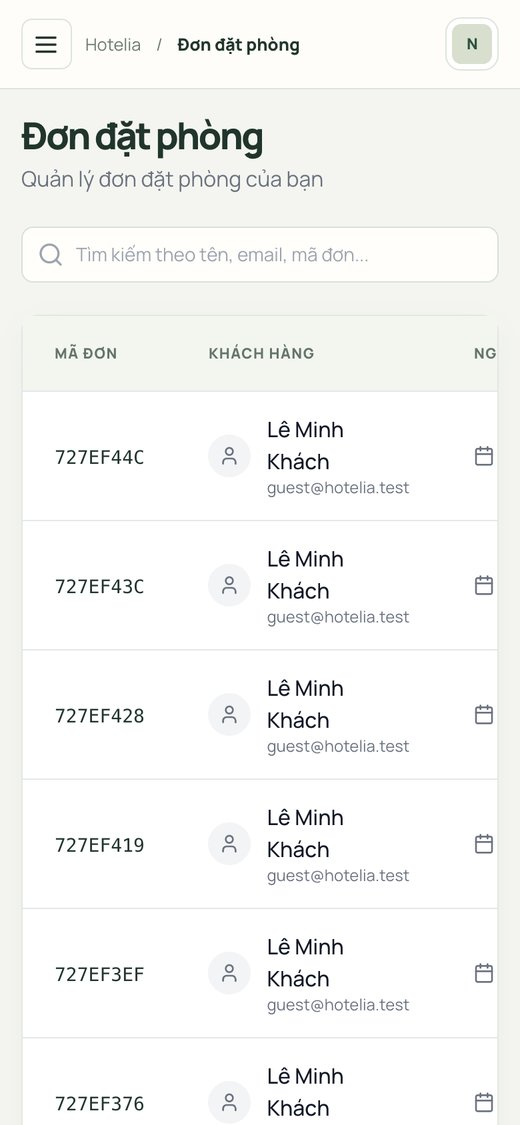
\includegraphics[height=7.5cm]{figures/shots/web-15-owner-bookings-mobile.jpg}}\hspace{1cm}
\subcaptionbox{Quản lý khách sạn, 768$\times$1024}{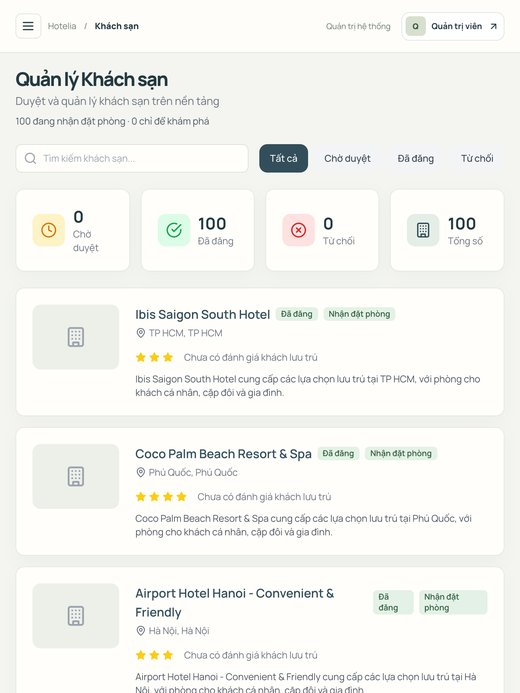
\includegraphics[height=7.5cm]{figures/shots/web-16-admin-hotels-tablet.jpg}}
\caption{Bảng điều khiển ở kích thước điện thoại và máy tính bảng}\label{fig:web-responsive}
\end{figure}

\section{Kiểm thử thành phần gợi ý}\label{sec:test-rec}

\subsection{Kiểm thử tự động}

\Cref{tab:test-rec} là các ca kiểm thử của thành phần gợi ý. Nhóm R01--R11 kiểm tra cách ly dữ liệu và ghi nhận tương tác. Nhóm R12--R13 kiểm tra cơ chế dự phòng. Nhóm R14--R17 kiểm tra khớp Python -- TypeScript. Nhóm R18--R22 kiểm tra bộ xếp hạng theo nội dung.

\begin{rtable}
\begin{longtable}{|C{1.2cm}|L{9.6cm}|C{1.6cm}|}
\caption{Ca kiểm thử thành phần gợi ý}\label{tab:test-rec}\\
\hline
\thead{Mã} & \thead{Kịch bản} & \thead{Kết quả} \\ \hline
\endfirsthead
\hline
\thead{Mã} & \thead{Kịch bản} & \thead{Kết quả} \\ \hline
\endhead
TC-R01 & Người dùng đăng nhập: chỉ dùng lịch sử \code{user:id}, không dùng \code{session} & Đạt \\ \hline
TC-R02 & Khách ẩn danh: không truy vấn đặt phòng của bất kỳ ai & Đạt \\ \hline
TC-R03 & Xếp hạng toàn bộ ứng viên trước khi cắt theo \code{limit} & Đạt \\ \hline
TC-R04 & Giữ bộ lọc điểm đến dù lịch sử nghiêng về thành phố khác & Đạt \\ \hline
TC-R05 & Mở lại cùng khách sạn không tăng số lượt xem & Đạt \\ \hline
TC-R06 & Lượt mở chỉ gắn vào lượt hiển thị khi đúng tác nhân, mã và ứng viên & Đạt \\ \hline
TC-R07 & Lượt hiển thị giữ thứ tự, tối đa 8, không bị ghi đè khi gửi lại & Đạt \\ \hline
TC-R08 & Từ chối ứng viên trùng hoặc chưa duyệt & Đạt \\ \hline
TC-R09 & Không lưu văn bản tìm kiếm tự do & Đạt \\ \hline
TC-R10 & Không gắn nhãn ``đã mở'' cho khách sạn không hiển thị hoặc người dùng khác & Đạt \\ \hline
TC-R11 & Xóa cả lượt xem và lượt hiển thị của một tác nhân & Đạt \\ \hline
TC-R12 & Mô hình không chấm được: dùng bộ xếp hạng nội dung, \code{modelUsed = false} & Đạt \\ \hline
TC-R13 & Mô hình chấm được: báo đúng \code{version}, \code{modelUsed = true} & Đạt \\ \hline
TC-R14 & Khớp điểm số Python -- TypeScript trên 5 véc-tơ (9 chữ số) & Đạt \\ \hline
TC-R15 & Khớp 16 đặc trưng trên 2 kịch bản, 8 khách sạn (9 chữ số) & Đạt \\ \hline
TC-R16 & Đặc trưng giờ theo giờ Việt Nam với \code{TZ=UTC} và \code{TZ=America/Los\_Angeles} & Đạt \\ \hline
TC-R17 & Nạp mô hình đang phục vụ và xếp hạng & Đạt \\ \hline
TC-R18 & Khởi động lạnh: đa dạng thành phố, không bịa đánh giá & Đạt \\ \hline
TC-R19 & Ưu tiên khách sạn tương tự về thành phố, tiện nghi, giá & Đạt \\ \hline
TC-R20 & Chuẩn hóa bí danh thành phố (TP HCM, Sài Gòn) và dấu & Đạt \\ \hline
TC-R21 & Một đánh giá 5 sao không vượt khách sạn có nhiều đánh giá tốt & Đạt \\ \hline
TC-R22 & Thiếu giá, không rõ hạng sao: không sinh NaN, không mất ứng viên & Đạt \\ \hline
\end{longtable}
\end{rtable}

\subsection{Tệp mô hình lỗi}

\Cref{tab:test-artifact} là kết quả khi cố ý làm hỏng tệp mô hình trong một bản sao của thư mục build. Trong mọi trường hợp lỗi, \code{rank} trả về \code{undefined}, nên API dùng bộ xếp hạng dự phòng; một cảnh báo cho biết nguyên nhân được ghi vào nhật ký. Trường hợp M5 cho thấy lỗi xuất hiện lúc chấm điểm (tệp nạp được nhưng cây hỏng) cũng được bắt.

\begin{table}[H]
\centering
\caption{Hành vi khi tệp mô hình bị lỗi}\label{tab:test-artifact}
\begin{rtable}
\begin{tabular}{|C{1.0cm}|L{3.6cm}|C{1.6cm}|L{3.2cm}|L{4.6cm}|}
\hline
\thead{Mã} & \thead{Tình huống} & \thead{Nạp được} & \thead{Xếp hạng} & \thead{Cảnh báo ghi nhận} \\ \hline
M1 & Tệp hợp lệ & có & LightGBM & -- \\ \hline
M2 & Không phải JSON & không & dự phòng & lỗi phân tích JSON \\ \hline
M3 & Đảo thứ tự đặc trưng & không & dự phòng & Model feature contract does not match backend \\ \hline
M4 & Không có cây & không & dự phòng & Model has no trees \\ \hline
M5 & Nút cây thiếu nhánh & có & dự phòng & Invalid LightGBM tree node \\ \hline
M6 & Tệp bị xóa & không & dự phòng & ENOENT \\ \hline
\end{tabular}
\end{rtable}
\end{table}

\section{Đánh giá mô hình LightGBM}\label{sec:eval-model}

\subsection{Thiết lập}

Ba phiên bản mô hình đã được huấn luyện. Cả ba dùng cùng 16 đặc trưng và mục tiêu LambdaRank, nhưng khác nhau về dữ liệu và cách đánh giá (\cref{tab:model-versions}). Mọi số liệu đều là đánh giá ngoại tuyến trên dữ liệu sinh trước phát hành, không phải số đo trên người dùng thật.

\begin{rtable}
\begin{longtable}{|L{3.8cm}|L{3.5cm}|L{3.5cm}|L{3.8cm}|}
\caption{Thiết lập của ba phiên bản mô hình}\label{tab:model-versions}\\
\hline
\thead{Khía cạnh} & \thead{v1 (23/10)} & \thead{v2 (23/10)} & \thead{v3 (24/10, đang phục vụ)} \\ \hline
\endfirsthead
\hline
\thead{Khía cạnh} & \thead{v1 (23/10)} & \thead{v2 (23/10)} & \thead{v3 (24/10, đang phục vụ)} \\ \hline
\endhead
Thuộc tính khách sạn & Sinh bằng hàm băm & Sinh bằng hàm băm & Ảnh chụp API (giá trị thật của danh mục) \\ \hline
Lịch sử mô phỏng & Một hồ sơ ưa thích cố định & Tín hiệu có trọng số như máy chủ, 1--12 tín hiệu & Như v2, 1--50 tín hiệu, 90 ngày \\ \hline
Nhóm ứng viên & 8 & 8 & 8; theo thành phố; toàn bộ 100 \\ \hline
Số truy vấn & 8.000 (6.800 / 1.200) & 8.000 (6.800 / 1.200) & 20.000 (14.000 / 3.000 / 3.000) \\ \hline
Tập báo cáo & Kiểm định (dùng cả để dừng sớm) & Kiểm định (dùng cả để dừng sớm) & Kiểm tra riêng \\ \hline
Đường cơ sở & quality\_prior & quality\_prior & quality\_prior, bộ xếp hạng nội dung, oracle \\ \hline
Giờ trong đặc trưng & Giờ của máy chủ & Giờ của máy chủ & Giờ Việt Nam \\ \hline
Số cây (best iteration) & 7 & 41 & 10 \\ \hline
\end{longtable}
\end{rtable}

\subsection{Kết quả}

\Cref{tab:model-results} tổng hợp kết quả của ba phiên bản. Với v1 và v2, mỗi truy vấn chỉ có 8 ứng viên, nên Hit@10 luôn bằng 1 kể cả với thứ tự ngẫu nhiên và không được dùng để so sánh.

\begin{table}[H]
\centering
\caption{Kết quả đánh giá ngoại tuyến các phiên bản mô hình}\label{tab:model-results}
\begin{rtable}
\begin{tabular}{|L{1.5cm}|L{4.1cm}|C{2.1cm}|C{2.1cm}|C{2.1cm}|L{2.4cm}|}
\hline
\thead{Phiên bản} & \thead{Phương pháp} & \thead{MRR@10} & \thead{NDCG@10} & \thead{Hit@10} & \thead{Tập đo} \\ \hline
\multirow{2}{*}{v1} & Đường cơ sở quality\_prior & 0,342 & 0,496 & 1,000 & \multirow{2}{*}{Kiểm định} \\ \cline{2-5}
 & LightGBM & 0,620 & 0,713 & 1,000 & \\ \hline
\multirow{2}{*}{v2} & Đường cơ sở quality\_prior & 0,373 & 0,520 & 1,000 & \multirow{2}{*}{Kiểm định} \\ \cline{2-5}
 & LightGBM & 0,539 & 0,650 & 1,000 & \\ \hline
\multirow{4}{*}{v3} & Đường cơ sở quality\_prior & 0,286 & 0,405 & 0,796 & \multirow{4}{2.4cm}{Kiểm tra, 3.000 truy vấn} \\ \cline{2-5}
 & Bộ xếp hạng nội dung (dự phòng) & 0,416 & 0,526 & 0,879 & \\ \cline{2-5}
 & LightGBM & 0,415 & 0,524 & 0,871 & \\ \cline{2-5}
 & Oracle (lợi ích kỳ vọng, không nhiễu) & 0,424 & 0,534 & 0,884 & \\ \hline
\end{tabular}
\end{rtable}
\end{table}

\Cref{tab:model-groups} chia kết quả v3 theo loại nhóm ứng viên. Nhóm \code{full\_catalog} (100 ứng viên) là nơi Hit@10 có ý nghĩa, vì chỉ 10\% ứng viên lọt vào top 10.

\begin{table}[H]
\centering
\caption{MRR@10 của v3 theo loại nhóm ứng viên (tập kiểm tra)}\label{tab:model-groups}
\begin{rtable}
\begin{tabular}{|L{2.8cm}|C{1.5cm}|C{1.8cm}|C{1.8cm}|C{1.9cm}|C{2.1cm}|C{1.6cm}|}
\hline
\thead{Nhóm} & \thead{Truy vấn} & \thead{Ứng viên TB} & \thead{Quality} & \thead{Nội dung} & \thead{LightGBM} & \thead{Oracle} \\ \hline
sample\_8 & 1.311 & 8 & 0,335 & 0,519 & 0,529 & 0,537 \\ \hline
destination & 1.106 & 8,8 & 0,363 & 0,414 & 0,407 & 0,414 \\ \hline
full\_catalog & 583 & 100 & 0,029 & 0,190 & 0,176 & 0,191 \\ \hline
\multicolumn{3}{|l|}{Hit@10 của nhóm full\_catalog} & 0,084 & 0,458 & 0,419 & 0,480 \\ \hline
\end{tabular}
\end{rtable}
\end{table}

\subsection{Phân tích}

\paragraph{Chênh lệch lớn ở v1, v2 đến từ cách đánh giá.} Ở v1 và v2, LightGBM hơn đường cơ sở 0,17--0,28 điểm MRR. Tuy nhiên đường cơ sở đó là \code{quality\_prior}, chỉ xét chất lượng khách sạn và hoàn toàn bỏ qua lịch sử. Trong khi đó, nhãn được sinh chủ yếu từ độ phù hợp với lịch sử (hệ số của \code{city\_affinity} là 1,75 so với 0,7 của \code{quality\_prior}). Một mô hình chỉ cần học ``ưu tiên khách sạn cùng thành phố với lịch sử'' là đã vượt đường cơ sở này. Ngoài ra, số liệu được báo cáo trên chính tập dùng để chọn số cây, nên có thiên lệch lạc quan nhỏ. Kết quả của v1 cao hơn v2 cũng không có nghĩa v1 tốt hơn: dữ liệu v1 dùng một hồ sơ ưa thích cố định, tạo ra quan hệ đơn giản hơn giữa đặc trưng và nhãn.

\paragraph{Với v3, LightGBM ngang bộ xếp hạng nội dung.} Khi so với bộ xếp hạng nội dung, tức chính cơ chế dự phòng của hệ thống, LightGBM v3 đạt MRR@10 0,415 so với 0,416. Chênh lệch này không đáng kể. LightGBM nhỉnh hơn ở nhóm 8 ứng viên (0,529 so với 0,519) nhưng kém hơn ở nhóm 100 ứng viên (0,176 so với 0,190). Cả hai đều rất gần mức oracle 0,424. Mức oracle là thứ tự theo đúng hàm lợi ích dùng để sinh nhãn, nên là giới hạn trên mà không mô hình nào vượt được trên tập dữ liệu này.

\paragraph{Vì sao mức trần thấp.} Oracle chỉ đạt 0,424 vì nhãn có nhiễu Gumbel: ngay cả khi biết chính xác lợi ích kỳ vọng, khách sạn tốt nhất cũng chỉ được chọn với một xác suất nhất định. Điều này mô phỏng việc người dùng thật không luôn chọn phương án ``tối ưu''.

\paragraph{Vì sao LightGBM không vượt bộ xếp hạng nội dung.} Hàm sinh nhãn là tổ hợp tuyến tính của các đặc trưng gần giống công thức của bộ xếp hạng nội dung: cùng thành phố, giá, sao, tiện nghi, chất lượng. Dữ liệu vì vậy không chứa quy luật nào mà công thức viết tay chưa nắm được. Mức độ quan trọng của đặc trưng (\cref{fig:importance}) xác nhận điều này. \code{city\_affinity} chiếm 44,6\% tổng độ lợi; tiếp theo là \code{price\_relative} 13,9\% và \code{price\_affinity} 12,8\%. Các đặc trưng thời gian gần như không được dùng: \code{hour\_sin} 0,5\%, \code{is\_weekend} 0\%. Kết quả này phù hợp với việc hàm sinh nhãn chỉ cộng 0,12 cho tiện nghi gia đình vào cuối tuần.

\begin{figure}[H]
\centering
\diagram{importance}
\caption{Tỷ lệ độ lợi (gain) của từng đặc trưng trong mô hình v3}\label{fig:importance}
\end{figure}

\paragraph{Kết luận về mô hình.} Các thực nghiệm chứng minh được bốn điều: (i) đường ống huấn luyện -- xuất -- phục vụ hoạt động đầu-cuối; (ii) mã TypeScript tái hiện chính xác điểm số và đặc trưng của Python; (iii) mô hình học được quy luật có trong dữ liệu, sát giới hạn trên; (iv) cơ chế dự phòng hoạt động khi mô hình lỗi. Các thực nghiệm không chứng minh rằng LightGBM gợi ý tốt hơn bộ xếp hạng nội dung, cũng không chứng minh rằng gợi ý làm tăng tỷ lệ đặt phòng của người dùng thật. Hai kết luận đó chỉ có thể rút ra từ dữ liệu hành vi thật và thử nghiệm A/B (\cref{sec:future}).

\subsection{Thí nghiệm phụ trên dữ liệu Trivago}\label{sec:trivago}

Trước khi xây dựng mô hình cho danh mục Hotelia, đồ án thử LambdaRank trên bộ dữ liệu Trivago RecSys Challenge 2019 \cite{adamczak2019} để kiểm tra phương pháp trên hành vi thật. Mỗi lượt bấm vào khách sạn (clickout) là một truy vấn; các khách sạn trong danh sách hiển thị là ứng viên. 18 đặc trưng chỉ dùng thông tin có trước lượt bấm (vị trí, giá, thứ hạng giá, tương tác trước đó trong phiên, thiết bị, giờ). Mô hình huấn luyện trên mẫu 100.000 hành động đầu tiên, chọn số cây trên 15\% phiên mới nhất của tập huấn luyện, rồi đánh giá trên một tập thời gian muộn hơn.

\begin{table}[H]
\centering
\caption{Kết quả thí nghiệm phụ trên Trivago RecSys 2019 (tập thời gian muộn hơn)}\label{tab:trivago}
\begin{rtable}
\begin{tabular}{|L{6.8cm}|C{2.0cm}|C{2.0cm}|C{2.0cm}|C{1.8cm}|}
\hline
\thead{Phương pháp} & \thead{MRR@10} & \thead{NDCG@10} & \thead{Hit@10} & \thead{Truy vấn} \\ \hline
B0: giữ thứ tự hiển thị gốc & 0,389 & 0,472 & 0,744 & 7.055 \\ \hline
B1: tần suất bấm theo (thành phố, khách sạn) & 0,313 & 0,412 & 0,737 & 7.068 \\ \hline
B2: độ phổ biến thành phố + số tiện nghi & 0,263 & 0,343 & 0,607 & 7.068 \\ \hline
LightGBM LambdaRank (B6, 43 cây) & 0,521 & 0,597 & 0,842 & 7.055 \\ \hline
\end{tabular}
\end{rtable}
\end{table}

Trên hành vi thật của Trivago, LightGBM hơn thứ tự hiển thị gốc 0,13 điểm MRR@10 (\cref{tab:trivago}). Kết quả này cho thấy phương pháp có giá trị khi dữ liệu chứa quy luật thật. Tuy nhiên, mô hình này không thể dùng cho Hotelia: mã khách sạn Trivago không ánh xạ được sang danh mục Hotelia, và đặc trưng được mô hình dùng để chia nút nhiều nhất (206 lần) là vị trí trong danh sách hiển thị gốc của Trivago, vốn không tồn tại trong Hotelia.

\section{Đánh giá chung}\label{sec:overall}

\subsection{Kết quả đạt được và ưu điểm}

\begin{itemize}
\item Tính đúng của đặt phòng được kiểm chứng trên cơ sở dữ liệu thật. Tình huống hai khách tranh căn phòng cuối, thử lại, hết hạn giữ và hủy được kiểm tra bằng giao dịch MongoDB thật, không chỉ bằng mô hình giả lập.
\item Bảo mật theo nguyên tắc ``không tin máy khách''. Số tiền thanh toán, trạng thái thanh toán, vai trò và quyền sở hữu đều được quyết định ở máy chủ. Quá trình kiểm tra lại khi viết báo cáo phát hiện và sửa một lỗ hổng thật (refresh token dùng như access token).
\item Gợi ý chạy trong cùng tiến trình, có dự phòng và có kiểm thử khớp. Không cần thêm dịch vụ, độ trễ mạng hay chi phí vận hành. Mọi lỗi của mô hình đều được chuyển sang dự phòng.
\item Trung thực về dữ liệu. Giao diện phân biệt điểm biên tập với đánh giá đã xác minh; báo cáo phân biệt dữ liệu thật với dữ liệu mô phỏng.
\item Triển khai thật. API, bảng điều khiển và cơ sở dữ liệu đang chạy với tên miền \code{hotelia.asia}; việc cập nhật mô hình có quy trình và đã được thực hiện.
\end{itemize}

\subsection{Giới hạn}\label{sec:limitations}

\begin{rtable}
\begin{longtable}{|C{0.7cm}|L{4.2cm}|L{9.8cm}|}
\caption{Các giới hạn của hệ thống}\label{tab:limitations}\\
\hline
\thead{\#} & \thead{Giới hạn} & \thead{Mô tả và hệ quả} \\ \hline
\endfirsthead
\hline
\thead{\#} & \thead{Giới hạn} & \thead{Mô tả và hệ quả} \\ \hline
\endhead
1 & Dữ liệu huấn luyện là dữ liệu sinh & Nhãn đến từ hàm lợi ích giả định; mô hình chưa học từ hành vi thật. Chưa có A/B test. Không thể kết luận về hiệu quả trên người dùng. \\ \hline
2 & Danh mục mô phỏng một phần & 80/100 khách sạn có giá, tồn kho, chủ khách sạn sinh tự động; điểm đánh giá là dữ liệu biên tập; số đánh giá đã xác minh trên môi trường vận hành bằng 0. \\ \hline
3 & Chưa có hoàn tiền tự động & \code{refund} trả 503; \code{calculateRefund} chưa được dùng; đặt phòng đã thanh toán payOS không thể xác nhận hủy qua hệ thống. \\ \hline
4 & payOS chưa kiểm thử với giao dịch thật & Chỉ có kiểm thử đơn vị với khóa thử; chưa có bằng chứng giao dịch thành công trên môi trường vận hành. \\ \hline
5 & Trạng thái chưa dùng & PAID, REFUNDED, COMPLETED được khai báo nhưng chưa có luồng; bảng \code{roomavailabilities} còn trong mã nhưng không dùng. \\ \hline
6 & Sign in with Apple phụ thuộc tài khoản trả phí & Bản build với tài khoản miễn phí ẩn nút Apple; luồng Apple mới được kiểm thử ở mức đơn vị. \\ \hline
7 & Quên mật khẩu phụ thuộc dịch vụ email & Cần cấu hình \code{RESET\_EMAIL\_WEBHOOK\_URL}; nếu chưa cấu hình, chức năng trả 503. \\ \hline
8 & Bảng điều khiển chỉ có tiếng Việt & Chưa có i18n cho web; nội dung dữ liệu chủ yếu tiếng Việt. \\ \hline
9 & Hạ tầng gói miễn phí & Render tạm dừng khi không có lưu lượng; yêu cầu đầu tiên có thể chờ hơn 20 giây. Chưa có giám sát, cảnh báo, sao lưu được cấu hình trong mã. \\ \hline
10 & Chưa kiểm thử tải và kiểm thử giao diện tự động & Chưa đo thông lượng, độ trễ dưới tải; chưa có XCUITest, Playwright. \\ \hline
11 & Chưa có cơ chế xin đồng ý thu thập dữ liệu & Dữ liệu tương tác được tối thiểu hóa và tự xóa, nhưng chưa có màn hình xin đồng ý theo Nghị định 13/2023/NĐ-CP. \\ \hline
\end{longtable}
\end{rtable}

\subsection{Rủi ro}

\begin{itemize}
\item Rủi ro vận hành thanh toán: nếu địa chỉ webhook bị chặn hoặc máy chủ đang ngủ khi payOS gửi webhook, đặt phòng có thể hết hạn giữ dù khách đã trả tiền. Hệ thống đã xử lý tình huống tiền về sau hạn bằng cách chuyển sang CANCEL\_REQUESTED, nhưng việc hoàn tiền vẫn phải làm thủ công.
\item Rủi ro dữ liệu: catalog thay đổi (giá, khách sạn mới) mà không huấn luyện lại sẽ làm phân phối đặc trưng lúc phục vụ lệch dần khỏi lúc huấn luyện.
\item Rủi ro bảo mật: refresh token cũ (không có \code{typ}) còn được chấp nhận tới khi hết hạn 7 ngày sau bản sửa. Mỗi tài khoản chỉ giữ một refresh token, nên đăng nhập trên thiết bị thứ hai làm phiên trên thiết bị thứ nhất hết hiệu lực khi access token hết hạn.
\end{itemize}

\section{Hướng phát triển}\label{sec:future}

\begin{enumerate}
\item Dữ liệu hành vi thật có đồng thuận. Bổ sung màn hình xin đồng ý thu thập dữ liệu tương tác cho mục đích gợi ý, cho phép rút lại đồng ý; dùng lượt hiển thị, lượt mở chi tiết, giữ phòng và đặt phòng đã xác nhận làm nhãn nhiều mức (ví dụ mở = 1, giữ = 2, xác nhận = 3). Cần hiệu chỉnh thiên lệch vị trí khi học từ nhật ký \cite{joachims2017}.
\item Thử nghiệm A/B. Chia ngẫu nhiên người dùng giữa bộ xếp hạng nội dung và LightGBM. Chỉ số chính là tỷ lệ đặt phòng được xác nhận trên mỗi lượt hiển thị; chỉ số bảo vệ là tỷ lệ hủy và độ trễ phản hồi \cite{kohavi2009}. Chỉ bật mô hình cho toàn bộ người dùng khi chênh lệch có ý nghĩa thống kê.
\item Giám sát mô hình và hệ thống. Ghi \code{ranking.mode} và \code{version} của mỗi phản hồi để theo dõi tỷ lệ rơi về dự phòng; theo dõi phân phối đặc trưng để phát hiện lệch; giám sát sức khỏe API, lỗi 5xx và thời gian phản hồi; nâng cấp gói hạ tầng để tránh khởi động lạnh.
\item Kho đặc trưng (feature store). Khi số khách sạn và người dùng tăng, tính sẵn các đặc trưng theo khách sạn và theo người dùng, dùng chung cho huấn luyện và phục vụ để loại bỏ lệch về định nghĩa.
\item Thanh toán trực tuyến đầy đủ. Cấu hình khóa payOS trên môi trường vận hành, kiểm thử bằng giao dịch thật giá trị nhỏ, cài đặt hoàn tiền theo \code{calculateRefund} với đối soát, và chuyển trạng thái REFUNDED.
\item Tối ưu tập ứng viên. Với danh mục lớn, thêm giai đoạn lọc thô (ví dụ theo khoảng cách, giá, độ phổ biến) để chỉ chấm điểm vài trăm ứng viên; lưu đệm danh mục đã lọc.
\item Đa dạng hóa kết quả. Áp dụng xếp hạng lại theo độ đa dạng (thành phố, mức giá, loại hình) cho cả đầu ra của LightGBM, không chỉ cho bộ xếp hạng dự phòng \cite{carbonell1998}.
\item Bảo mật môi trường vận hành. Hỗ trợ nhiều refresh token theo thiết bị kèm phát hiện tái sử dụng; thu hồi chủ động token cũ không có \code{typ}; chuyển refresh token trên web sang cookie \code{HttpOnly}; bổ sung giới hạn tần suất riêng cho \code{/auth}; quét phụ thuộc định kỳ; đối chiếu với OWASP ASVS \cite{owaspasvs}.
\item Hoàn thiện sản phẩm. Bản tiếng Anh cho bảng điều khiển; dịch nội dung khách sạn; trạng thái COMPLETED tự động sau khi trả phòng; thông báo đẩy; phát hành TestFlight; kiểm thử giao diện tự động; thay chuyển hướng ở \code{hotelia.asia} bằng trang giới thiệu sản phẩm.
\end{enumerate}

\section{Kết luận chương}

Chương này đã trình bày kết quả của 57 ca kiểm thử máy chủ, 80 ca kiểm thử Python, kịch bản tranh chấp trên MongoDB thật, 13 ca phân quyền và 7 ca phiên đăng nhập qua HTTP, 6 kịch bản lỗi mô hình và 18 ca kiểm thử giao diện. Quá trình kiểm thử phát hiện và sửa năm lỗi giao diện cùng một lỗ hổng xác thực. Đánh giá mô hình cho thấy LightGBM v3 học sát giới hạn của dữ liệu sinh nhưng không vượt bộ xếp hạng nội dung. Vì vậy đánh giá ngoại tuyến hiện tại chỉ xác nhận tính đúng của đường ống, chưa xác nhận hiệu quả gợi ý.

\fronttitle{Kết luận}

\section*{Kết quả đạt được}

Đồ án đã xây dựng và triển khai Hotelia, một nền tảng đặt phòng khách sạn gồm ứng dụng iOS song ngữ viết bằng SwiftUI theo mô hình MVVM, máy chủ NestJS với MongoDB, bảng điều khiển React cho chủ khách sạn và quản trị viên, và thành phần gợi ý khách sạn dựa trên LightGBM LambdaRank. Hệ thống đang chạy với API tại \code{api.hotelia.asia} (Render), bảng điều khiển tại \code{admin.hotelia.asia} (Vercel) và cơ sở dữ liệu MongoDB Atlas, phục vụ danh mục 100 khách sạn tại 14 điểm đến.

Đối chiếu với bốn câu hỏi nghiên cứu nêu ở phần Mở đầu:

\begin{enumerate}[label=Q\arabic*., leftmargin=1.4cm]
\item Chống bán trùng và lũy đẳng. Việc kết hợp quy ước ngày nửa mở, đếm phòng trống theo từng đêm, giao dịch MongoDB với tài liệu khóa theo loại phòng và khóa \code{Idempotency-Key} có băm nội dung đã ngăn được bán trùng và đặt phòng trùng. Điều này được kiểm chứng trên MongoDB thật, trong đó hai khách tranh căn phòng cuối thì chỉ một người thành công, và các yêu cầu gửi lại cùng khóa chỉ tạo một đặt phòng.
\item Xác thực, phân quyền và thanh toán an toàn. Máy chủ tự xác minh ID token của Google và Apple, phân quyền ba vai trò kết hợp kiểm tra quyền sở hữu, và chỉ xác nhận thanh toán payOS qua webhook có chữ ký với số tiền khớp. Quá trình đối chiếu khi viết báo cáo đã phát hiện và sửa hai lỗ hổng: refresh token dùng được thay access token, và refresh token cũ vẫn dùng được sau khi xoay vòng do bcrypt chỉ đọc 72 byte đầu. 13 ca phân quyền và 7 ca phiên đăng nhập qua HTTP đều đạt.
\item Gợi ý chạy trong NestJS. Đường ống lọc ứng viên, ghi nhận lượt hiển thị và lượt mở chi tiết, tính 16 đặc trưng và chấm điểm mô hình LightGBM từ tệp JSON hoạt động trong chính tiến trình NestJS mà không cần dịch vụ Python. Điểm số và từng đặc trưng khớp với Python tới 9 chữ số thập phân. Mọi lỗi của tệp mô hình đều được chuyển sang bộ xếp hạng dự phòng.
\item Ý nghĩa của MRR, NDCG trên dữ liệu trước phát hành. Phiên bản v2 đạt MRR@10 = 0,539 và NDCG@10 = 0,650, so với 0,373 và 0,520 của đường cơ sở chất lượng. Khi đánh giá chặt hơn ở v3 (tập kiểm tra riêng, so với bộ xếp hạng nội dung và mức oracle), LightGBM đạt MRR@10 = 0,415, ngang bộ xếp hạng nội dung (0,416) và gần giới hạn trên của dữ liệu (0,424). Các con số này xác nhận đường ống hoạt động đúng và mô hình học được quy luật của dữ liệu sinh. Chúng không chứng minh mô hình gợi ý tốt hơn trên người dùng thật.
\end{enumerate}

\section*{Giới hạn}

Đồ án có các giới hạn sau, đã được trình bày chi tiết ở \cref{sec:limitations}:
\begin{itemize}
\item Mô hình gợi ý chưa được huấn luyện hay đánh giá trên hành vi người dùng thật và chưa qua thử nghiệm A/B. Vì vậy chưa thể khẳng định mô hình cải thiện trải nghiệm hay tỷ lệ đặt phòng.
\item 80 trong 100 khách sạn có giá, tồn kho và chủ khách sạn mô phỏng; điểm đánh giá hiển thị là điểm biên tập.
\item Thanh toán payOS chưa được kiểm thử với giao dịch thật; hoàn tiền tự động chưa được cài đặt.
\item Sign in with Apple phụ thuộc tài khoản Apple Developer Program trả phí khi triển khai thật.
\item Bảng điều khiển web chỉ có tiếng Việt; chưa có kiểm thử tải và kiểm thử giao diện tự động; hạ tầng đang dùng gói miễn phí.
\end{itemize}

\section*{Hướng phát triển}

Bước tiếp theo quan trọng nhất là thu thập dữ liệu hành vi có sự đồng ý của người dùng, rồi huấn luyện lại mô hình bằng nhãn thật và so sánh với bộ xếp hạng nội dung qua thử nghiệm A/B. Song song là các việc hoàn thiện sản phẩm: kích hoạt và kiểm thử thanh toán trực tuyến, cài đặt hoàn tiền, giám sát mô hình và hệ thống, tối ưu tập ứng viên khi danh mục lớn lên, đa dạng hóa kết quả gợi ý, hoàn thiện bảo mật môi trường vận hành và bổ sung bản tiếng Anh cho bảng điều khiển.


\printbibliography[heading=bibintoc,title={Tài liệu tham khảo}]

\end{document}
